%Page Setup, don't remove
\documentclass[12pt]{book} 
\setlength{\columnsep}{0.7truecm}
\setlength{\parindent}{0cm}
\usepackage[top=2truecm,bottom=2.8truecm, left=2.2truecm, right=2.2truecm,headsep=10pt, paperwidth=19.3truecm, paperheight=27.6truecm]{geometry} 
\usepackage[usenames,dvipsnames]{xcolor}
\usepackage{tcolorbox}
\definecolor{ocre}{RGB}{52,177,201} 
\usepackage{pdfpages}
\usepackage{avant}
\usepackage{bussproofs}
\usepackage{mathptmx}
%\usepackage{ebgaramond}
% \usepackage{xeCJK}
% \setCJKmainfont{SimSun}
\usepackage{tikz}
\usepackage{tkz-euclide}
\usepackage{matchsticks}
\usepackage{wrapfig}
\usepackage{listings}
\usepackage[utf8]{vietnam}
\usepackage{babel}
\usepackage[LSBC5,T1]{fontenc}

%----------------------------------------------------------------------------------------
%	VARIOUS REQUIRED PACKAGES
%----------------------------------------------------------------------------------------
\usepackage{titlesec} % Allows customization of titles
\usepackage{multicol}
\usepackage{graphicx} % Required for including pictures
%\graphicspath{{Pictures/}} % Specifies the directory where pictures are stored
\usepackage{lipsum} % Inserts dummy text
\usepackage{tikz} % Required for drawing custom shapes
%\usepackage{enumitem} % Customize lists
%\setlist{nolistsep} % Reduce spacing between bullet points and numbered lists
\usepackage{booktabs} % Required for nicer horizontal rules in tables
\usepackage{eso-pic} % Required for specifying an image background in the title page
\usepackage{titletoc} % Required for manipulating the table of contents
\contentsmargin{0cm} % Removes the default margin
\usepackage{adjustbox} 
\usepackage{amsmath,amsfonts,amssymb,amsthm} % For math equations, theorems, symbols, etc
%\usepackage[framemethod=tikz]{mdframed} 
\usepackage[sexy]{evan}
\usepackage{hyperref}
\urlstyle{same}
\usepackage{tikz} % figure in two column
\usepackage{float}
\usepackage{biblatex}
\usepackage{caption}% dinh dang figure caption
%\usepackage[font=normalsize]{caption}
\usepackage{changepage}
\usepackage{booktabs}

\usepackage{chngcntr}
\usepackage{array}
\usepackage{eurosym}
\usepackage{multirow}
\usepackage{mathtools}
\usepackage{setspace}
\usepackage{afterpage}
\usepackage{scalerel}
\usepackage{blindtext}
\usepackage{tabularx}
\usepackage{afterpage}
\usepackage{array}
%\usepackage{transparent}
\usepackage{efbox}
\usepackage{tabulary}
% \usepackage{CJKutf8}
\usepackage{subcaption}
\usepackage{rotating}
\usepackage{microtype}
\usepackage{pgfplots}

\usetikzlibrary{lindenmayersystems}
\usetikzlibrary{shapes,shapes.geometric}
\usetikzlibrary{decorations.pathreplacing}
\usetikzlibrary{calc,intersections}
\usetikzlibrary[shadings]
\usetikzlibrary{decorations.fractals}

\newmdenv[skipabove=7pt,
skipbelow=7pt,
backgroundcolor=black!5,
linecolor=ocre,
leftline=true,
innerleftmargin=6pt,
innerrightmargin=6pt,
innertopmargin=8pt,
leftmargin=0cm,
rightmargin=0cm,
innerbottommargin=8pt]{tBox}

\def\PIbox#1{\tikz\node[draw = ocre,fill=black!5,align=justify,text width=.95\linewidth,inner sep=2mm]{#1};}%
\renewcommand{\qedsymbol}{}	
\usepackage{fancyhdr} % Required for header and footer configuration
%%%% Header for duong vao toan hoc
\fancypagestyle{duongvaotoanhoc}{
	\fancyhf{}
	\fancyhead[E]{
		\insertpic{63}{740}{1}{duongvao1}
		\insertpic{333}{35}{1}{fduongvao1}
}
	\fancyhead[O]{
		\insertpic{1}{740}{1}{duongvao2}
		\insertpic{59}{34.9}{1}{fduongvao2}
}	
\renewcommand{\footrulewidth}{0pt}
\fancyfoot[LE,RO]{\sffamily\footnotesize	\thepage}

\fancyfoot[LO,RE]{\sffamily\scriptsize TẬP 6 -- SỐ 12 THÁNG 12/2022}
}

\fancypagestyle{duongvaotoanhocnone}{
	\fancyhf{}
	\fancyhead[E]{
		\insertpic{333}{35}{1}{fduongvao1}
	}
	\fancyhead[O]{
		\insertpic{59}{34.9}{1}{fduongvao2}
	}	
	\renewcommand{\footrulewidth}{0pt}
	\fancyfoot[LE,RO]{\sffamily\footnotesize	\thepage}
	
	\fancyfoot[LO,RE]{\sffamily\scriptsize TẬP 6 -- SỐ 12 THÁNG 12/2022}
}

\fancypagestyle{thachthuctoanhoc}{
	\fancyhf{}
	\fancyhead[E]{
		\insertpic{63}{740}{1}{thachthuc1}
		\insertpic{333}{35}{1}{fthachthuc1}
	}
	\fancyhead[O]{
		\insertpic{1}{740}{1}{thachthuc2}
		\insertpic{59}{34.9}{1}{fthachthuc2}
	}	
	\renewcommand{\footrulewidth}{0pt}
	\fancyfoot[LE,RO]{\sffamily\footnotesize	\thepage}
	
	\fancyfoot[LO,RE]{\sffamily\scriptsize TẬP 6 -- SỐ 12 THÁNG 12/2022}
}

\fancypagestyle{thachthuctoanhocnone}{
	\fancyhf{}
	\fancyhead[E]{
		\insertpic{333}{35}{1}{fthachthuc1}
	}
	\fancyhead[O]{
		\insertpic{59}{34.9}{1}{fthachthuc2}
	}	
	\renewcommand{\footrulewidth}{0pt}
	\fancyfoot[LE,RO]{\sffamily\footnotesize	\thepage}
	
	\fancyfoot[LO,RE]{\sffamily\scriptsize TẬP 6 -- SỐ 12 THÁNG 12/2022}
}


%%%% Header for Toán học và đời sống
\fancypagestyle{toanhocvadoisong}{
			\fancyhf{}
		\fancyhead[E]{
			\insertpic{63}{740}{1}{toanhocds1}
			\insertpic{333}{35}{1}{ftoanhocds1}
		}
		\fancyhead[O]{
			\insertpic{1}{740}{1}{toanhocds2}
			\insertpic{59}{34.9}{1}{ftoanhocds2}
		}	
		\renewcommand{\footrulewidth}{0pt}
		\fancyfoot[LE,RO]{\sffamily\footnotesize	\thepage}
		
		\fancyfoot[LO,RE]{\sffamily\scriptsize TẬP 6 -- SỐ 12 THÁNG 12/2022}
}
\fancypagestyle{toanhocvadoisongnone}{
	\fancyhf{}
	\fancyhead[E]{
		\insertpic{333}{35}{1}{ftoanhocds1}
	}
	\fancyhead[O]{
		\insertpic{59}{34.9}{1}{ftoanhocds2}
	}	
	\renewcommand{\footrulewidth}{0pt}
	\fancyfoot[LE,RO]{\sffamily\footnotesize	\thepage}
	
	\fancyfoot[LO,RE]{\sffamily\scriptsize TẬP 6 -- SỐ 12 THÁNG 12/2022}
}

\fancypagestyle{doisongtoanhoc}{
	\fancyhf{}
	\fancyhead[E]{
		\insertpic{63}{740}{1}{dstoanhoc1}
		\insertpic{333}{35}{1}{fdstoanhoc1}
	}
	\fancyhead[O]{
		\insertpic{1}{740}{1}{dstoanhoc2}
		\insertpic{59}{34.9}{1}{fdstoanhoc2}
	}	
	\renewcommand{\footrulewidth}{0pt}
	\fancyfoot[LE,RO]{\sffamily\footnotesize	\thepage}
	
	\fancyfoot[LO,RE]{\sffamily\scriptsize TẬP 6 -- SỐ 12 THÁNG 12/2022}
}
\fancypagestyle{doisongtoanhocnone}{
	\fancyhf{}
	\fancyhead[E]{
		\insertpic{333}{35}{1}{fdstoanhoc1}
	}
	\fancyhead[O]{
		\insertpic{59}{34.9}{1}{fdstoanhoc2}
	}	
	\renewcommand{\footrulewidth}{0pt}
	\fancyfoot[LE,RO]{\sffamily\footnotesize	\thepage}
	
	\fancyfoot[LO,RE]{\sffamily\scriptsize TẬP 6 -- SỐ 12 THÁNG 12/2022}
}

%%% doi thoai toan hoc
\fancypagestyle{doithoaitoanhoc}{
	\fancyhf{}
	\fancyhead[E]{
		\insertpic{63}{740}{1}{doithoai1}
		\insertpic{333}{35}{1}{fdoithoai1}
	}
	\fancyhead[O]{
		\insertpic{1}{740}{1}{doithoai2}
		\insertpic{59}{34.9}{1}{fdoithoai2}
	}	
	\renewcommand{\footrulewidth}{0pt}
	\fancyfoot[LE,RO]{\sffamily\footnotesize	\thepage}
	
	\fancyfoot[LO,RE]{\sffamily\scriptsize TẬP 6 -- SỐ 12 THÁNG 12/2022}
}
\fancypagestyle{doithoaitoanhocnone}{
	\fancyhf{}
	\fancyhead[E]{
		\insertpic{333}{35}{1}{fdoithoai1}
	}
	\fancyhead[O]{
		\insertpic{59}{34.9}{1}{fdoithoai2}
	}	
	\renewcommand{\footrulewidth}{0pt}
	\fancyfoot[LE,RO]{\sffamily\footnotesize	\thepage}
	
	\fancyfoot[LO,RE]{\sffamily\scriptsize TẬP 6 -- SỐ 12 THÁNG 12/2022}
}

%%%% Header for co dien hien dai
\fancypagestyle{codienhiendai}{
	\fancyhf{}
	\fancyhead[E]{
		\insertpic{63}{740}{1}{codien1}
		\insertpic{333}{35}{1}{fcodien1}
	}
	\fancyhead[O]{
		\insertpic{1}{740}{1}{codien2}
		\insertpic{59}{34.9}{1}{fcodien2}
	}	
	\renewcommand{\footrulewidth}{0pt}
	\fancyfoot[LE,RO]{\sffamily\footnotesize	\thepage}
	
	\fancyfoot[LO,RE]{\sffamily\scriptsize TẬP 6 -- SỐ 12 THÁNG 12/2022}
}
\fancypagestyle{codienhiendainone}{
	\fancyhf{}
	\fancyhead[E]{
		\insertpic{333}{35}{1}{fcodien1}
	}
	\fancyhead[O]{
		\insertpic{59}{34.9}{1}{fcodien2}
	}	
	\renewcommand{\footrulewidth}{0pt}
	\fancyfoot[LE,RO]{\sffamily\footnotesize	\thepage}
	
	\fancyfoot[LO,RE]{\sffamily\scriptsize TẬP 6 -- SỐ 12 THÁNG 12/2022}
}

\fancypagestyle{diendandayvahoctoan}{
	\fancyhf{}
	\fancyhead[E]{
		\insertpic{63}{740}{1}{diendan1}
		\insertpic{333}{35}{1}{fdiendan1}
	}
	\fancyhead[O]{
		\insertpic{1}{740}{1}{diendan2}
		\insertpic{59}{34.9}{1}{fdiendan2}
	}	
	\renewcommand{\footrulewidth}{0pt}
	\fancyfoot[LE,RO]{\sffamily\footnotesize	\thepage}
	
	\fancyfoot[LO,RE]{\sffamily\scriptsize TẬP 6 -- SỐ 12 THÁNG 12/2022}
}
\fancypagestyle{diendandayvahoctoannone}{
	\fancyhf{}
	\fancyhead[E]{
		\insertpic{333}{35}{1}{fdiendan1}
	}
	\fancyhead[O]{
		\insertpic{59}{34.9}{1}{fdiendan2}
	}	
	\renewcommand{\footrulewidth}{0pt}
	\fancyfoot[LE,RO]{\sffamily\footnotesize	\thepage}
	
	\fancyfoot[LO,RE]{\sffamily\scriptsize TẬP 6 -- SỐ 12 THÁNG 12/2022}
}

\fancypagestyle{cackithitoan}{
	\fancyhf{}
	\fancyhead[E]{
		\insertpic{63}{740}{1}{cackithi1}
		\insertpic{333}{35}{1}{fcackithi1}
	}
	\fancyhead[O]{
		\insertpic{1}{740}{1}{cackithi2}
		\insertpic{59}{34.9}{1}{fcackithi2}
	}	
	\renewcommand{\footrulewidth}{0pt}
	\fancyfoot[LE,RO]{\sffamily\footnotesize	\thepage}
	
	\fancyfoot[LO,RE]{\sffamily\scriptsize TẬP 6 -- SỐ 12 THÁNG 12/2022}
}
\fancypagestyle{cackithitoannone}{
	\fancyhf{}
	\fancyhead[E]{
		\insertpic{333}{35}{1}{fcackithi1}
	}
	\fancyhead[O]{
		\insertpic{59}{34.9}{1}{fcackithi2}
	}	
	\renewcommand{\footrulewidth}{0pt}
	\fancyfoot[LE,RO]{\sffamily\footnotesize	\thepage}
	
	\fancyfoot[LO,RE]{\sffamily\scriptsize TẬP 6 -- SỐ 12 THÁNG 12/2022}
}

\fancypagestyle{lichsutoanhoc}{
	\fancyhf{}
	\fancyhead[E]{
		\insertpic{63}{740}{1}{lichsu1}
		\insertpic{333}{35}{1}{flichsu1}
	}
	\fancyhead[O]{
		\insertpic{1}{740}{1}{lichsu2}
		\insertpic{59}{34.9}{1}{flichsu2}
	}	
	\renewcommand{\footrulewidth}{0pt}
	\fancyfoot[LE,RO]{\sffamily\footnotesize	\thepage}
	
	\fancyfoot[LO,RE]{\sffamily\scriptsize TẬP 6 -- SỐ 12 THÁNG 12/2022}
}
\fancypagestyle{lichsutoanhocnone}{
	\fancyhf{}
	\fancyhead[E]{
		\insertpic{333}{35}{1}{flichsu1}
	}
	\fancyhead[O]{
		\insertpic{59}{34.9}{1}{flichsu2}
	}	
	\renewcommand{\footrulewidth}{0pt}
	\fancyfoot[LE,RO]{\sffamily\footnotesize	\thepage}
	
	\fancyfoot[LO,RE]{\sffamily\scriptsize TẬP 6 -- SỐ 12 THÁNG 12/2022}
}

%%%% Header for Tìm hiểu khoa học
\fancypagestyle{timhieukhoahoc}{
		\fancyhf{}
	\fancyhead[E]{
		\insertpic{63}{740}{1}{timhieu1}
		\insertpic{333}{35}{1}{ftimhieu1}
	}
	\fancyhead[O]{
		\insertpic{1}{740}{1}{timhieu2}
		\insertpic{59}{34.9}{1}{ftimhieu2}
	}	
	\renewcommand{\footrulewidth}{0pt}
	\fancyfoot[LE,RO]{\sffamily\footnotesize	\thepage}
	
	\fancyfoot[LO,RE]{\sffamily\scriptsize TẬP 6 -- SỐ 12 THÁNG 12/2022}	
}
\fancypagestyle{timhieukhoahocnone}{
	\fancyhf{}
	\fancyhead[E]{
		\insertpic{333}{35}{1}{ftimhieu1}
	}
	\fancyhead[O]{
		\insertpic{59}{34.9}{1}{ftimhieu2}
	}	
	\renewcommand{\footrulewidth}{0pt}
	\fancyfoot[LE,RO]{\sffamily\footnotesize	\thepage}
	
	\fancyfoot[LO,RE]{\sffamily\scriptsize TẬP 6 -- SỐ 12 THÁNG 12/2022}	
}

%%%% Header for quan toan
\fancypagestyle{quantoan}{
		\fancyhf{}
		\fancyhead[E]{
		\insertpic{63}{740}{1}{quantoan1}
		\insertpic{333}{35}{1}{fquantoan1}
	}
	\fancyhead[O]{
		\insertpic{1}{740}{1}{quantoan2}
		\insertpic{59}{34.9}{1}{fquantoan2}
	}	
	\renewcommand{\footrulewidth}{0pt}
	\fancyfoot[LE,RO]{\sffamily\footnotesize	\thepage}
	
	\fancyfoot[LO,RE]{\sffamily\scriptsize TẬP 6 -- SỐ 12 THÁNG 12/2022}
}
\fancypagestyle{quantoannone}{
	\fancyhf{}
	\fancyhead[E]{
		\insertpic{333}{35}{1}{fquantoan1}
	}
	\fancyhead[O]{
		\insertpic{59}{34.9}{1}{fquantoan2}
	}	
	\renewcommand{\footrulewidth}{0pt}
	\fancyfoot[LE,RO]{\sffamily\footnotesize	\thepage}
	
	\fancyfoot[LO,RE]{\sffamily\scriptsize TẬP 6 -- SỐ 12 THÁNG 12/2022}
}


\fancypagestyle{hoccungpi}{
				\fancyhf{}
		\fancyhead[E]{
			\insertpic{63}{740}{1}{hoccungpi1}
			\insertpic{333}{35}{1}{fhoccungpi1}
		}
		\fancyhead[O]{
			\insertpic{1}{740}{1}{hoccungpi2}
			\insertpic{59}{34.9}{1}{fhoccungpi2}
		}	
		\renewcommand{\footrulewidth}{0pt}
		\fancyfoot[LE,RO]{\sffamily\footnotesize	\thepage}
		
		\fancyfoot[LO,RE]{\sffamily\scriptsize TẬP 6 -- SỐ 12 THÁNG 12/2022}	
}
\fancypagestyle{hoccungpinone}{
	\fancyhf{}
	\fancyhead[E]{
		\insertpic{333}{35}{1}{fhoccungpi1}
	}
	\fancyhead[O]{
		\insertpic{59}{34.9}{1}{fhoccungpi2}
	}	
	\renewcommand{\footrulewidth}{0pt}
	\fancyfoot[LE,RO]{\sffamily\footnotesize	\thepage}
	
	\fancyfoot[LO,RE]{\sffamily\scriptsize TẬP 6 -- SỐ 12 THÁNG 12/2022}	
}

\fancypagestyle{toancuabi}{
	\fancyhf{}
	\fancyhead[E]{
		\insertpic{63}{740}{1}{toancuabi1}
		\insertpic{333}{35}{1}{ftoancuabi1}
	}
	\fancyhead[O]{
		\insertpic{1}{740}{1}{toancuabi2}
		\insertpic{59}{34.9}{1}{ftoancuabi2}
	}	
	\renewcommand{\footrulewidth}{0pt}
	\fancyfoot[LE,RO]{\sffamily\footnotesize	\thepage}
	
	\fancyfoot[LO,RE]{\sffamily\scriptsize TẬP 6 -- SỐ 12 THÁNG 12/2022}	
}
\fancypagestyle{toancuabinone}{
	\fancyhf{}
	\fancyhead[E]{
		\insertpic{333}{35}{1}{ftoancuabi1}
	}
	\fancyhead[O]{
		\insertpic{59}{34.9}{1}{ftoancuabi2}
	}	
	\renewcommand{\footrulewidth}{0pt}
	\fancyfoot[LE,RO]{\sffamily\footnotesize	\thepage}
	
	\fancyfoot[LO,RE]{\sffamily\scriptsize TẬP 6 -- SỐ 12 THÁNG 12/2022}	
}

\fancypagestyle{gocco}{
	\fancyhf{}
	\fancyhead[E]{
		\insertpic{63}{740}{1}{gocco1}
		\insertpic{333}{35}{1}{fgocco1}
	}
	\fancyhead[O]{
		\insertpic{1}{740}{1}{gocco2}
		\insertpic{59}{34.9}{1}{fgocco2}
	}	
	\renewcommand{\footrulewidth}{0pt}
	\fancyfoot[LE,RO]{\sffamily\footnotesize	\thepage}
	
	\fancyfoot[LO,RE]{\sffamily\scriptsize TẬP 6 -- SỐ 12 THÁNG 12/2022}	
}

\fancypagestyle{gocconone}{
	\fancyhf{}
	\fancyhead[E]{
		\insertpic{333}{35}{1}{fgocco1}
	}
	\fancyhead[O]{
		\insertpic{59}{34.9}{1}{fgocco2}
	}	
	\renewcommand{\footrulewidth}{0pt}
	\fancyfoot[LE,RO]{\sffamily\footnotesize	\thepage}
	
	\fancyfoot[LO,RE]{\sffamily\scriptsize TẬP 6 -- SỐ 12 THÁNG 12/2022}	
}
	
%	\fancyfoot[C]{\sffamily\footnotesize Tạp chí Pi } % Print the nearest section name on the left side of odd pages	


\pagestyle{fancy}
\renewcommand{\chaptermark}[1]{\markboth{\normalsize\bfseries\chaptername\ \thechapter.\ #1}{}} % Chapter text font settings
\renewcommand{\sectionmark}[1]{\markright{\normalsize\thesection\hspace{5pt}#1}{}} % Section text font settings


\fancyfoot[LE,RO]{\sffamily\footnotesize	\thepage} % Font setting for the page number in the header
\fancyfoot[LO,RE]{\sffamily\footnotesize TẬP 6 -- SỐ 12 THÁNG 12/2022 \LARGE  $\pmb{\pi}$}


\fancyfoot[C]{\sffamily\footnotesize Tạp chí Pi } % Print the nearest section name on the left side of odd pages
\renewcommand{\headrulewidth}{0pt} % Width of the rule under the header
\addtolength{\headheight}{2.5pt} % Increase the spacing around the header slightly
\renewcommand{\footrulewidth}{.5pt} % Removes the rule in the footer


\fancypagestyle{plain}{\fancyhead{}\renewcommand{\headrulewidth}{0pt}} % Style for when a plain pagestyle is specified

% Removes the header from odd empty pages at the end of chapters
\makeatletter
\renewcommand{\cleardoublepage}{
	\clearpage\ifodd\c@page\else
	\hbox{}
	\vspace*{\fill}
	\thispagestyle{empty}
	\newpage
	\fi}


\graphicspath{{../main/pic/}}
\everymath{\displaystyle}
\DeclareMathAlphabet{\pazocal}{OMS}{zplm}{m}{n}
\usepackage{ebgaramond}
\usepackage{xpatch}
\PassOptionsToPackage{hyphens}{url}

\usepackage{url}
\usepackage{type1cm}
\usepackage{lettrine}
\usepackage{makecell}
\renewcommand{\LettrineTextFont}{\rmfamily}
\usepackage{skak}
%\usepackage{xskak}
\usepackage{tabularx}
\usepackage{microtype}
\usepackage{cases}
\usepackage{tikz-cd}
\usepackage{oplotsymbl}
\definecolor{codienhiendai}{cmyk}{0.72, 0, 0.42, 0.1}
\definecolor{thachthuctoanhoc}{cmyk}{0.87, 0.46, 0.69, 0.31}
\definecolor{diendantoanhoc}{cmyk}{0.75, 0, 0.7, 0}
\definecolor{timhieukhoahoc}{cmyk}{0.84, 0.7, 0, 0}
\definecolor{quantoan}{cmyk}{0.8, 0.57, 0, 0}
\definecolor{cackithi}{cmyk}{0.7, 0.35, 0, 0}
\definecolor{hoccungpi}{cmyk}{0.67, 0.6, 0, 0}
\definecolor{gocco}{cmyk}{0.65, 0.78, 0, 0}
\definecolor{toancuabi}{cmyk}{0, 1, 0, 0}
\definecolor{doithoaitoanhoc}{cmyk}{0.6, 0.3, 0 ,0.63}
\definecolor{duongvaotoanhoc}{cmyk}{0, 0.7, 0.9, 0}
\definecolor{toanhocdoisong}{cmyk}{0 , 0.93, 1, 0}
\definecolor{tramthienvan}{cmyk}{0, 0.98, 0.95, 0}
\definecolor{lichsutoanhoc}{cmyk}{0.35, 0.5, 0.8, 0.1}
\definecolor{doisongtoanhoc}{cmyk}{0.25, 0.3, 0.5, 0.1}
\definecolor{amber}{rgb}{1.0, 0.75, 0.0}

\definecolor{darkblue}{rgb}{0.089,0.21,0.363}
\usepackage[hang,splitrule]{footmisc}
\usetikzlibrary{arrows}
\usetikzlibrary{patterns}
\usetikzlibrary{decorations.pathreplacing,calligraphy,backgrounds}
\setlength{\footnotemargin}{0cm}
\setlength{\footnotesep}{0.35cm}
\setlength{\skip\footins}{0.35cm}
\setlength\footskip{33pt}

\newcommand\blfootnote[1]{%
	\begingroup
	\renewcommand\thefootnote{}\footnote{#1}%
	\addtocounter{footnote}{-1}%
	\endgroup
}

\def\footnotelayout{\itshape}
\renewcommand*\footnoterule{}
\renewcommand\footnoterule{\vspace*{0.25cm}\hrule width 1\textwidth\vspace*{0.25cm}}

\newcommand{\insertpic}[4]{
	\begingroup
	\AddToShipoutPicture*{\put(#1,#2){\includegraphics[scale=#3]{#4}}} % %Image background
	\centering
	\endgroup
}

\tikzset{
	squarednode/.style={rectangle, draw=red!60, fill=red!5, very thick, minimum size=3mm}
}

\tikzset{
	sqnode/.style={rectangle, draw=cackithi, very thick, minimum size=3mm}
}

\tikzset{
	roundnode/.style={circle, draw=toancuabi, fill=cackithi!50, minimum size=3mm},
}


\begin{document}
%	 \thispagestyle{empty}
%	 \begingroup 
%	 \AddToShipoutPicture*{\put(0,0){\includegraphics[scale=1]{ML.pdf}}}
%	 \centering
%	 \vspace*{0cm}
%	 \endgroup
%	 \newpage	  
%	 \pagestyle{empty}
%
	\setcounter{page}{2}
	
	\setcounter{figure}{0}
	\thispagestyle{toanhocvadoisongnone}
\pagestyle{toanhocvadoisong}
\everymath{\color{toanhocdoisong}}
\graphicspath{{../toanhocdoisong/pic/}}
\begingroup
\blfootnote{$^1$\color{toanhocdoisong}Nguồn: Accromath, vol. $17$, $2022$.}
%\blfootnote{$^2$\color{toanhocdoisong}Đại học McGill, Canada.}
%\blfootnote{$^3$\color{toanhocdoisong}École Polytechnique Fédérale de Lausanne, Thụy Sỹ.}
\blfootnote{$^2$\color{toanhocdoisong}Viện Toán học.}

\AddToShipoutPicture*{\put(0,616){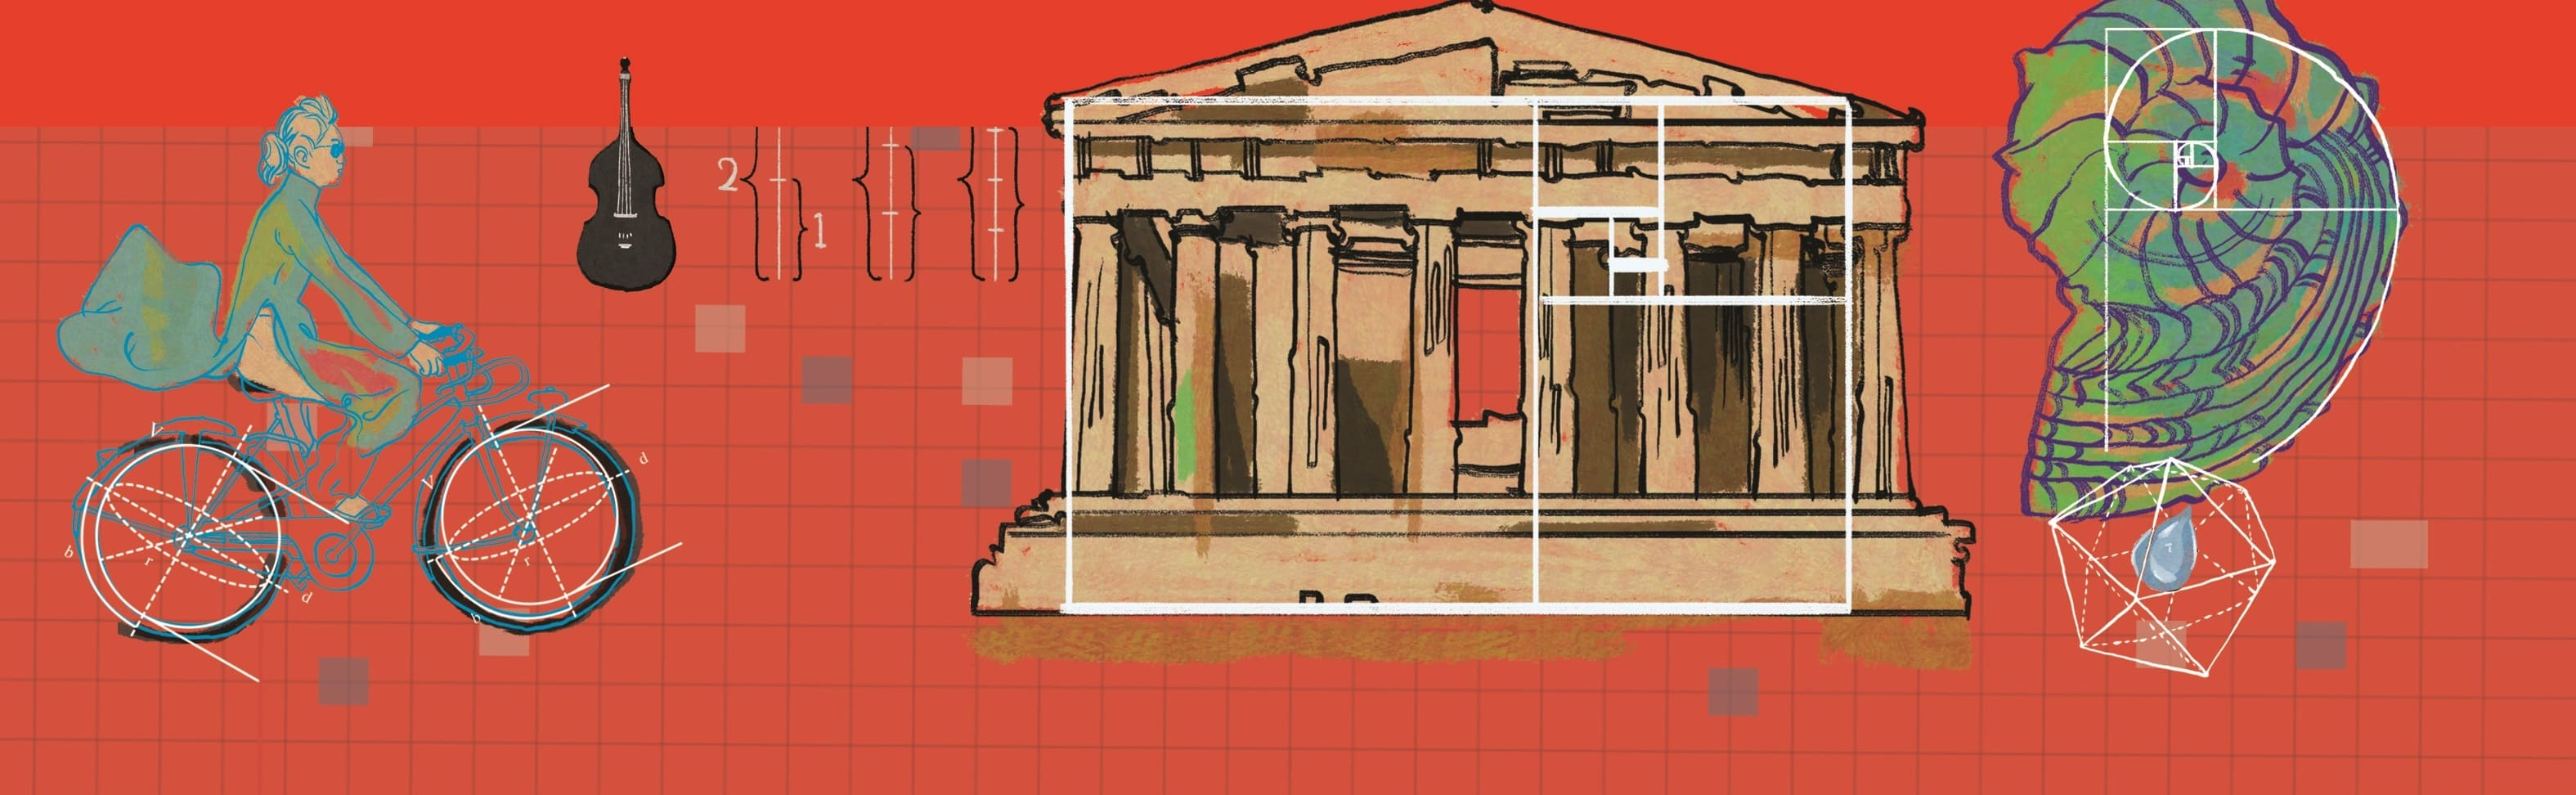
\includegraphics[width=19.3cm]{../bannertoanhocdoisong}}}
\AddToShipoutPicture*{\put(102,507){
\includegraphics[scale=1]{../tieude.pdf}}}
\centering
\endgroup

\vspace*{200pt}

\begin{multicols}{2}
	\textit{Khi các đấu thủ hoặc các đội thi đấu với nhau, cơ hội chiến thắng của mỗi bên phụ thuộc vào thực lực của họ. Hệ thống tính điểm Elo là một phương pháp tính toán trình độ tương đối của những người chơi trong một trò chơi có tổng bằng không, cho phép đánh giá khả năng về kết cục của một trận đấu.}
	\vskip 0.05cm
	\textbf{\color{toanhocdoisong}Xếp hạng Elo của các kỳ thủ cờ vua}
	\vskip 0.05cm
	Ngày nay, một người mới chơi có điểm số Elo khoảng $1000$, còn một người chơi nghiệp dư giỏi có điểm số Elo khoảng $2000$. Các đại kiện tướng quốc tế cần đạt được điểm số Elo tối thiểu $2500$. Nhóm này gần như trùng với nhóm các kỳ thủ chuyên nghiệp, ngày nay có hơn $1000$ người trên toàn thế giới. Cho đến nay chỉ có khoảng mười lăm kỳ thủ từng đạt đến mức điểm Elo $2800$ trong sự nghiệp của mình.
	\vskip 0.05cm
	Các phần mềm cờ vua cũng có xếp hạng điểm Elo. Chương trình tốt nhất hiện nay, Stockfish, có điểm số Elo khoảng $3700$, cho thấy trong cờ vua máy tính đã vượt xa con người như thế nào: xác suất $p_{AB}$ giữa Stockfish ($A$) và Magnus Carlsen ($B$) là khoảng $0{,}992\ldots$ (tức là trung bình $992$ trận thắng và $8$ trận thua cho máy tính sau $1000$ trận đấu không có hòa). Đó cũng là khoảng cách giữa Carlsen và một kỳ thủ nghiệp dư giỏi có điểm số Elo $2000$, mức đạt được bởi khoảng $30000$ người.
	\vskip 0.05cm
	Ta cũng có thể đặt câu hỏi liệu xếp hạng Elo có thể g  iúp so sánh các kỳ thủ thuộc các thời đại khác nhau. Chẳng hạn, một kỳ thủ có điểm Elo $2700$ trong thập niên $1980$ liệu có trình độ tương đương với một kỳ thủ có điểm Elo $2700$ ngày nay? Đây là một câu hỏi phức tạp, nhất là khi bản thân môn cờ vua cũng đã thay đổi. Chẳng hạn, các kỳ thủ, từ những người chuyên nghiệp đến những người nghiệp dư hăng hái nhất, đều dùng phần mềm để luyện tập. Nhưng người ta cũng quan sát được hiện tượng ``lạm phát", được gây ra bởi chính cách tính điểm Elo. Từ đầu những năm $2000$, điểm Elo trung bình của $50$ kỳ thủ mạnh nhất đã tăng hàng chục điểm, do đó điểm Elo cỡ $2700$ ở năm $2010$ rất có thể kém giá trị hơn so với ở năm $2000$.
	\vskip 0.05cm
	Từ ngày $24$ tháng $11$ đến ngày $16$ tháng $12$ năm $2021$, tại Dubai đã diễn ra giải vô địch thế giới môn cờ vua. Kỳ thủ Nauy Magnus Carlsen, nhà vô địch từ năm $2013$, đấu với kỳ thủ Nga Ian Nepomniachtchi, người giành chiến thắng ở Giải đấu các ứng viên\footnote[3]{\color{toanhocdoisong}Giải đấu để chọn ra người thách đấu với nhà vô địch -- Pi.}. Người chiến thắng giành được $1{,}2$ triệu euro tiền thưởng.
	\vskip 0.05cm
	Trận đấu gồm $14$ ván. Mỗi ván thắng được $1$ điểm, thua $0$ điểm và nếu hòa thì mỗi đấu thủ được $\frac{1}{2}$ điểm. Chung cuộc, Carlsen giành chiến thắng $7\frac{1}{2} - 3\frac{1}{2}$, với $4$ thắng, $0$ thua và $7$ hòa sau $11$ ván ($3$ ván cuối cùng không cần thiết vì không làm thay đổi kết quả cuối cùng). Và như vậy Carlsen giành danh hiệu vô địch thế giới lần thứ $5$ liên tiếp.
	\vskip 0.05cm
	Kết quả này phù hợp với hệ thống tính điểm Elo mà Liên đoàn Cờ vua Thế giới (FIDE) sử dụng từ năm $1970$ để đánh giá trình độ tương đối của các kỳ thủ. Quả thực, khi đó Carlsen được xếp hạng số một thế giới với số điểm Elo $2856$, trong khi đối thủ của anh, kỳ thủ số một của Nga, xếp thứ năm với số điểm Elo $2782$.
	\vskip 0.05cm
	Khi hai đấu thủ $A$ và $B$ với Elo $\theta_A$ và $\theta_B$ đấu với nhau, phương pháp Elo dự đoán $A$ sẽ giành được số điểm trung bình là
	\setlength{\abovedisplayskip}{4pt}
	\setlength{\belowdisplayskip}{4pt}
	\begin{align*}
		s_{AB} = \frac{1}{1+ 10^{-(\theta_A - \theta_B) /400}} \tag{$1$}
	\end{align*}
	biết rằng $A$ được $1$ điểm nếu thắng, $0$ nếu thua và $\frac{1}{2}$ nếu hòa. Điểm số trung bình B giành được là $s_{BA} = 1 – s_{AB}$.
	\vskip 0.05cm
	Trước trận tranh ngôi vô địch, ta có $\theta_A = 2856$ với Carlsen và $\theta_B = 2782$ với Nepomniachtchi, do đó $s_{AB} \approx 0{,}60$, tiên đoán chiến thắng của kỳ thủ Nauy vì trung bình anh sẽ giành được $8\frac{1}{2}$ điểm sau $14$ ván, so với số điểm $5\frac{1}{2}$ của kỳ thủ Nga.
	\vskip 0.05cm
	\textbf{\color{toanhocdoisong}Cơ sở toán học của phương pháp tính điểm Elo}
	\vskip 0.05cm
	Để xác định số điểm trung bình $s_{AB}$ của kỳ thủ $A$ khi đấu với kỳ thủ $B$, phương pháp ngây thơ là lấy số điểm trung bình của $A$ trong các trận đã đấu giữa hai người. Nhưng trong một trò chơi như cờ vua, phần lớn trong số hàng trăm nghìn người chơi chưa từng gặp nhau, và ngay cả khi họ đã từng gặp nhau, số trận họ đã đấu với nhau là quá ít để có một đánh giá chất lượng. Hệ thống tính điểm Elo giải quyết khó khăn này dựa vào một mô hình toán học cho phép xếp hạng các đấu thủ và qua đó ước tính kết quả có thể xảy ra khi họ đối đầu nhau.
	\vskip 0.02cm
	Biểu thức ($1$) lấy cảm hứng từ một mô hình được thiết lập từ những năm $1920$ bởi nhà toán học người Đức Ernst Zermelo và sau đó được cải tiến bởi nhà thống kê người Canada Ralph Bradley và người đồng nghiệp Milton Terry. Trong các công trình này, cũng như trong phần còn lại của bài viết, ta giả sử mọi ván đấu đều phân định thắng thua. Như vậy đây là một mô hình đơn giản hóa, nhất là đối với môn cờ vua, khi hòa là kết quả thường xảy ra nhất giữa các kỳ thủ đỉnh cao.
	\vskip 0.02cm
	Khi một ván đấu kết thúc với kết quả thắng $(1)$ hoặc thua $(0)$, điểm số trung bình chính là xác suất $p_{AB}$ để $A$ thắng $B$. Mô hình Bradley--Terry--Elo giả sử rằng xác suất này có dạng
	\begin{align*}
		p_{AB} = G(\theta_A - \theta_B)\tag{$2$}
	\end{align*}
	ở đó $G: \mathbb R \rightarrow (0, 1)$ là một hàm liên tục, tăng ngặt sao cho $G(x) + G(-x) = 1$ với mọi số thực $x$ và $G(x) \rightarrow 1$ khi $x \rightarrow \infty$. Một thí dụ về hàm như thế được cho trong Hình $1$. Ta có $p_{AB} + p_{BA} = G(\theta_A - \theta_B) + G(\theta_B - \theta_A) = 1$, không có kết quả hòa. Vì $G(0) = 1/2$, hai đấu thủ có trình độ ngang nhau có xác suất thắng như nhau; hiệu $\theta_A - \theta_B$ càng tăng thì xác suất để $A$ thắng càng lớn, và tiến tới giới hạn bằng $1$, nghĩa là chiến thắng chắc chắn của $A$.
	Lựa chọn phổ biến nhất của $G$ là luật logistic với tham số $\beta > 0$, được định nghĩa bởi
	
	\vspace{-15pt}
	\begin{align*}
		L(x) = \frac{ 1 }{ (1 + e^{-\beta x}) }\tag{$3$}
	\end{align*}
	với mọi $x \in \mathbb R$.
	\vskip 0.1cm
	Chọn $G = L$ với tham số $\beta = \ln(10) / 400$, ta thu được công thức ($1$) mà FIDE sử dụng. Ban đầu, nhà vật lý người Mỹ gốc Hungary Arpad Elo, người đưa phương pháp mô hình hóa này vào thế giới cờ vua, sử dụng một hàm phân phối chuẩn, khi đó $s_{AB}$ không có công thức tường minh như trên.
	\begin{figure}[H]
		\vspace*{-5pt}
		\centering
		\captionsetup{labelformat= empty, justification=centering}
		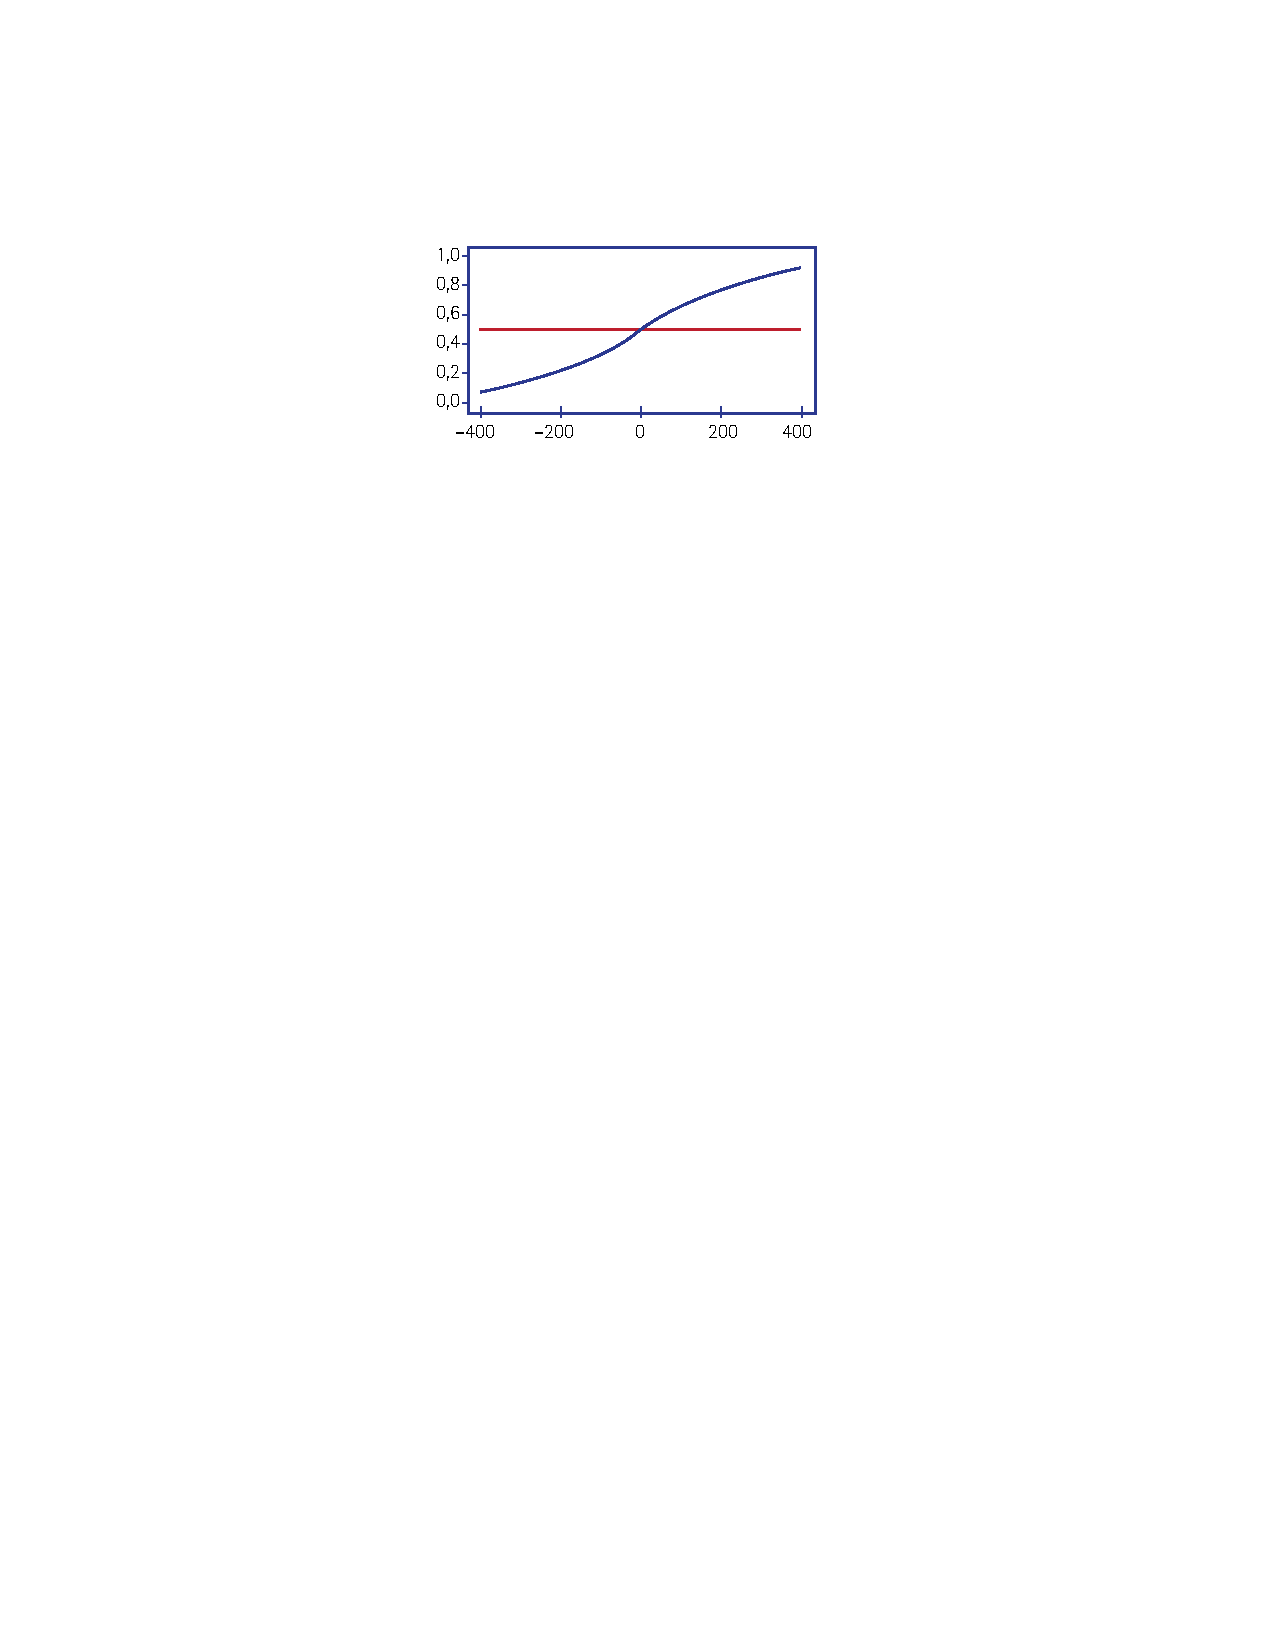
\includegraphics[width= 0.8\linewidth]{pic1}
		\caption{\small\textit{\color{toanhocdoisong}Hình $1$. Đồ thị hàm logistic $L(x)$ với $\beta = \ln(10) / 400$.}}
		\vspace*{-10pt}
	\end{figure}
	\textbf{\color{toanhocdoisong}Tính chất của mô hình xác suất}
	\vskip 0.05cm
	Mô hình Bradley--Terry--Elo có ưu điểm là nó cho phép xếp hạng tất cả người chơi của một trò chơi theo trình độ tương đối, ngay cả khi họ chưa từng đối đầu trực tiếp. Do đó, ta có thể dùng nó để dự đoán, đặc biệt là dựa vào các mô phỏng.
	Tuy nhiên, giả định rằng xác suất để $A$ thắng $B$ có dạng ($2$) không hề là một điều vô tình. Như đã đề cập, nó ngầm cho rằng không có ván hòa. Nếu có kết quả hòa, mô hình sẽ cần phải được điều chỉnh.
	\vskip 0.05cm
	Biểu thức ($2$) cũng ngầm giả định rằng kết quả một trận đấu giữa $A$ và $B$ chỉ phụ thuộc vào trình độ tương đối $\theta_A - \theta_B$. Đặc biệt, những yếu tố như đi trước (cầm quân trắng trong cờ vua), được nghỉ ngơi nhiều hơn đối thủ, hay thi đấu trước các cổ động viên không ảnh hưởng đến kết quả cuối cùng (một điều không hợp lý đối với thể thao chuyên nghiệp).
	\vskip 0.05cm
	Hơn nữa, cần phải hiểu rằng điểm số Elo của một đấu thủ không hề có giá trị nội tại: ý nghĩa của nó phụ thuộc vào điểm số Elo của các đối thủ, vì ta có thể cộng tất cả với cùng một hằng số tùy ý, hiệu số giữa chúng vẫn giữ nguyên. Tương tự, nếu ta nhân tất cả các Elo với một hằng số $c > 0$ và thay hàm $G(x)$ bởi $G(x / c)$, các xác suất thắng cũng không thay đổi.
	\vskip 0.05cm
	Trong trường hợp công thức ($1$), được biểu diễn trong Hình $1$ với các giá trị $\theta_A - \theta_B$ từ $-400$ đến $+400$, tham số $\beta$ được chọn sao cho chênh lệch $100$ điểm cho xác suất thắng $64\%$ đối với người mạnh hơn. Nếu chênh lệch là $200$ điểm, xác suất là $75\%$, và nó vào khoảng $91\%$ khi chênh lệch là $400$ điểm.
	\vskip 0.05cm
	Trong cờ vua, điểm Elo của hầu hết các kỳ thủ có trong xếp hạng của FIDE nằm trong khoảng từ $1000$ đến $3000$. Phân phối của chúng nói chung không đối xứng và thay đổi tùy theo từng nước. Hơn nữa, có nhiều phiên bản khác nhau của hệ thống xếp hạng, ngoài ra nó còn được điều chỉnh để áp dụng cho nhiều trò chơi và môn thể thao khác, trong đó có cờ vây, \textit{scrabble}, nhiều trò chơi trên mạng, bóng đá, tennis và khúc côn cầu trên băng.
	\vskip 0.05cm
	\textbf{\color{toanhocdoisong}Cập nhật xếp hạng}
	\vskip 0.05cm
	Tất nhiên là trình độ tương đối của các đấu thủ thay đổi theo thời gian. Một số người mạnh lên khi tích lũy thêm kinh nghiệm, một số khác yếu đi do tuổi tác, hoặc, trong trường hợp các môn thể thao đồng đội, do chấn thương, do giải nghệ hoặc do chuyển nhượng không tốt.
	\vskip 0.05cm
	Để thể hiện sự thay đổi này, phương pháp tính điểm Elo đưa ra một quy tắc cập nhật điểm xếp hạng sau mỗi trận đấu. Gọi $\theta_{A, n}$ và $\theta_{B, n}$ là điểm xếp hạng (Elo) của hai đấu thủ A và B ngay trước lần gặp nhau thứ $n$. Elo đề xuất rằng sau trận đấu này, chênh lệch $\theta_{A, n} - \theta_{B, n}$ được phân phối lại cho hai người theo ``độ bất ngờ" của kết quả và một số thực dương $k$, gọi là \textit{hệ số phát triển}.
	\vskip 0.05cm
	Gọi $s$ là kết quả của ván đấu giữa $A$ và $B$, với $s = 1$ nếu $A$ thắng, $s = 0$ nếu $A$ thua và $s = 1/2$ nếu ván đấu hòa. Elo mới của $A$ sẽ là
	\begin{align*}
		\theta_{A, n + 1} = \theta_{A, n} + k (s – s_{AB, n}),
	\end{align*}
	ở đó $s_{AB, n}$ là kết quả dự đoán được tính theo công thức ($1$) với các giá trị $\theta_{A, n}$ và $\theta_{B, n}$. Dễ thấy điểm số Elo của $A$ tăng nếu $s = 1$, và $s_{AB, n}$ càng nhỏ thì điểm số tăng càng nhiều. Như vậy, chiến thắng trước một đối thủ mạnh hơn thì có giá trị hơn. Tương tự, điểm số Elo của $A$ giảm khi thua, tức là khi $s = 0$. Cuối cùng, khi ván đấu hòa, điểm số Elo của $A$ tăng nếu điểm số Elo ban đầu của $B$ lớn hơn, tức là $s_{AB, n} < 1/2$.
	Đối với các kỳ thủ chuyên nghiệp, hệ thống tính điểm Elo cố định giá trị $k = 10$, do đó tại giải vô địch thế giới, mỗi ván thắng mang lại cho Carlsen $10 \times (1 – 0{,}60) \approx 4$ điểm Elo, trong khi mỗi ván hòa khiến anh mất $10 \times (0{,}5 – 0{,}60) \approx 1$ điểm. Sau giải đấu, điểm số Elo mới của anh là
	\begin{align*}
		2856 + 4 \times 4{,}0 - 7 \times 1{,}0 = 2865,
	\end{align*}
	trong khi đó điểm số Elo của Nepomniachtchi giảm từ $2782$ xuống $2773$.
	\vskip 0.05cm
	Các giá trị khác của $k$ được dùng cho các trình độ khác nhau của các kỳ thủ. Chẳng hạn, người ta dùng $k = 40$ cho các kỳ thủ mới chơi chưa quá $30$ ván hoặc các kỳ thủ trẻ dưới $18$ tuổi, giúp họ nhanh chóng đạt đến trình độ thực. Sau đó, $k$ được quy định bằng $20$ chừng nào điểm Elo của họ vẫn ở dưới $2400$.
	\vskip 0.05cm
	\textbf{\color{toanhocdoisong}Tính chất của phương pháp cập nhật}
	\vskip 0.05cm
	Trong trường hợp đặc biệt khi tất cả các ván đấu đều phân thắng bại, ta thấy rằng một cách tổng quát, phương pháp cập nhật mà Elo đề xuất sử dụng một hàm $M: \mathbb R \rightarrow (0, \infty)$ liên tục, giảm ngặt sao cho $M(x) \rightarrow 0$ khi $x \rightarrow \infty$. Hàm này cho phép cập nhật điểm xếp hạng của các đấu thủ $A$ và $B$ như sau.
	\vskip 0.05cm
	Nếu $A$ thắng:
	\begin{align*}
		&\theta_{A, n  +1} = \theta_{A, n} + M(\theta_{A, n} - \theta_{B, n}),\\
		&\theta_{B, n  +1} = \theta_{B, n} - M(\theta_{A, n} - \theta_{B, n}).
	\end{align*}
	Nếu $B$ thắng:
	\begin{align*}
		&\theta_{A, n  +1} = \theta_{A, n} - M(\theta_{B, n} - \theta_{A, n}),\\
		&\theta_{B, n  +1} = \theta_{B, n} + M(\theta_{B, n} - \theta_{A, n}).
	\end{align*}
	Trong công thức của FIDE, $M(x) = k L(-x)$ với mọi số thực $x$.
	\vskip 0.01cm
	Công thức cập nhật này có ý nghĩa tìm kiếm xác suất. Thực vậy, gọi $\theta_A$ và $\theta_B$ là trình độ tương đối thực sự nhưng chưa biết của hai đấu thủ $A$ và $B$. Giả sử $G(\theta_A - \theta_B)$ là xác suất thực sự để $A$ thắng $B$. Kỳ vọng của thay đổi xếp hạng của $A$ tại thời điểm $n$ được cho bởi biểu thức sau:
	\begin{align*}
		&M(\theta_{A, n} - \theta_{B, n}) G(\theta_A - \theta_B)\\
		&- M(\theta_{B, n} - \theta_{A, n}) G(\theta_B - \theta_A).
	\end{align*}
	Nếu phương pháp cập nhật là tốt, ta mong muốn rằng kỳ vọng này bằng $0$ khi $\theta_{A, n} - \theta_{B, n} = \theta_A - \theta_B$. Do $M$ là hàm giảm, ta cũng hy vọng rằng sau ván đấu, hiệu $(\theta_{A, n + 1} - \theta_{B, n + 1}) - (\theta_A - \theta_B)$ gần $0$ hơn so với hiệu $(\theta_{A, n} - \theta_{B, n}) - (\theta_A - \theta_B)$.
	\vskip 0.01cm
	Lập luận tương tự cũng đúng đối với $B$, và ta có thể kiểm tra rằng những tính chất mong muốn này được đạt nếu các hàm $G$ và $M$ thỏa mãn, với mọi số thực $x$:
	\begin{align*}
		M(x) / M(-x) = G(-x) / G(x). \tag{$4$}
	\end{align*}
	Từ phương trình cân bằng này, với một chút nỗ lực, ta có thể chứng minh rằng với mỗi hàm $M$ cho trước, hàm $G$ duy nhất thỏa mãn được cho bởi
	\begin{align*}
		G(x) = \frac { M(-x) }{ M(x) + M(-x) },
	\end{align*}
	với mọi $x \in \mathbb R$.
	\vskip 0.01cm
	Do đó, quy tắc cập nhật mà Elo đề xuất ngầm cho rằng xác suất ban đầu là xác suất logistic, tức là $G = L$.
	\vskip 0.01cm
	Có một lưu ý tinh tế: nếu ta cố định hàm $G$ trước thì tồn tại vô số hàm $M$ thỏa mãn quan hệ ($4$). Thật vậy, với mọi hằng số $k > 0$, $M(x) = k G(-x)$ là một nghiệm. Nhưng ta cũng có thể chọn $M(x) = k G(-x) S(|x|)$, ở đó $S$ là một hàm thỏa mãn $S(0) = 1$ và $S(x) = S(-x)$ với mọi số thực $x$. Tất nhiên là hàm $S$ được chọn phải đảm bảo tính đơn điệu giảm của $M$.
	\vskip 0.05cm
	\textbf{\color{toanhocdoisong}Kết quả về sự hội tụ}
	\vskip 0.05cm
	Có thể liên hệ phương pháp cập nhật của Elo với thuật toán giảm gradient ngẫu nhiên trong học máy trong một mô hình hồi quy logistic.
	\vskip 0.05cm
	Ta hãy tưởng tượng có $N$ đấu thủ và trình độ của họ được biểu diễn bởi vector $(\theta_1, \dots, \theta_N)$ ẩn nhưng cố định. Ta cũng giả sử rằng ban đầu, ta có một ước lượng $(\theta_{1, 0}, \dots, \theta_{N, 0})$, và các đấu thủ sẽ tham gia một dãy vô hạn các ván đấu, mỗi ván diễn ra giữa hai đấu thủ được chọn ngẫu nhiên theo phân phối đều. Cuối cùng, tưởng tượng rằng sau mỗi ván, vector trình độ được cập nhật theo phương pháp của Elo tại hai tọa độ $i$ và $j$ của hai đấu thủ vừa thi đấu.
	\vskip 0.05cm
	Dưới giả thiết các hàm $G$ và $M$ thỏa mãn các điều kiện đã nói đến ở trên, và hơn nữa $M$ có đạo hàm bị chặn, nhà toán học người Anh David Aldous đã chứng minh được rằng khi $n$ tiến ra vô cùng, dãy các vector $(\theta_{1, n}, \dots, \theta_{N, n})$ đạt đến một phân phối dừng. Liệu phân phối dừng này có phải là một xấp xỉ tốt của $(\theta_1, \dots, \theta_N)$ hay không vẫn là một câu hỏi lý thuyết mở, mặc dù nó đã được khẳng định bởi nhiều mô phỏng và thực tế hàng chục năm sử dụng hệ thống xếp hạng Elo của các kỳ thủ cờ vua.
	\vskip 0.05cm
	Trong khi đó, mặc dù kết quả hội tụ như của Aldous tạo niềm tin đối với phương pháp của Elo, chưa chắc đã tồn tại một vector ẩn $(\theta_1, \dots, \theta_N)$ phản ánh trình độ thực sự của các đấu thủ. Rốt cuộc thì các đấu thủ thay đổi theo thời gian, và các đội thể thao cũng liên tục thay đổi. Vector trình độ thực, nếu tồn tại, là một vector động.
	\vskip 0.05cm
	Thành công của phương pháp tính điểm Elo nằm ở khả năng theo được sự thay đổi này mà không phải phụ thuộc vào một mô hình ngẫu nhiên chính xác. Đây là một thực tế được xác nhận trong môn cờ vua, và trong cả nhiều tình huống khác, trong đó tham số $\beta$ và hệ số phát triển $k$ cần được lựa chọn một cách thích hợp.
	\vskip 0.05cm
	\textbf{\color{toanhocdoisong}Hệ thống Elo trong khúc côn cầu}
	\vskip 0.05cm
	Để minh họa phương pháp tính điểm Elo và khả năng dự đoán của nó ở ngoài môn cờ vua, ta hãy cùng xem xét ứng dụng của nó trong môn khúc côn cầu trên băng\footnote[4]{\color{toanhocdoisong}Accromath là tạp chí Canada, nơi khúc côn cầu trên băng là môn thể thao phổ biến nhất -- Pi.}, trong đó nhiều điều chỉnh đã được thực hiện để tận dụng kết quả của tất cả các trận trong vòng đấu thường và vòng đấu loại trực tiếp của giải National Hockey League (NHL) kể từ khi nó ra đời vào năm $1917$. Các dữ liệu này được lưu tại trang \url{hockey-reference.com}.
	\vskip 0.05cm
	Thí dụ, các nhà phân tích Ryan Best và Neil Paine của trang \textit{FiveThirtyEight} đề xuất một hệ thống xếp hạng Elo tính đến các tham số sau:
	\vskip 0.05cm
	$a)$ Mỗi đội có số diểm Elo ban đầu là $1380$.
	\vskip 0.05cm
	$b)$ Quy tắc cập nhật sử dụng hệ số phát triển $k = 6$.
	\vskip 0.05cm
	$c)$ Ta tính đến lợi thế sân nhà, tức là nếu hai đội có cùng Elo, đội chủ nhà có xác suất thắng là $57{,}1\%$ thay vì $50\%$.
	\vskip 0.05cm
	$d)$ Thay đổi điểm Elo tăng thêm $25\%$ đối với những trận loại trực tiếp.
	\vskip 0.05cm
	$e)$ Đầu mỗi mùa giải, điểm Elo của mỗi đội được tính lại, bằng
	\begin{align*}
		0{,}7 \!\times\!\text{điểm xếp hạng mùa trước} + 0{,}3 \!\times\!\! 1505.
	\end{align*}
	Như vậy, điểm số Elo trung bình của cả mùa giải dao động hàng năm xung quanh $1500$.
	\begin{figure}[H]
		\vspace*{-5pt}
		\centering
		\captionsetup{labelformat= empty, justification=centering}
		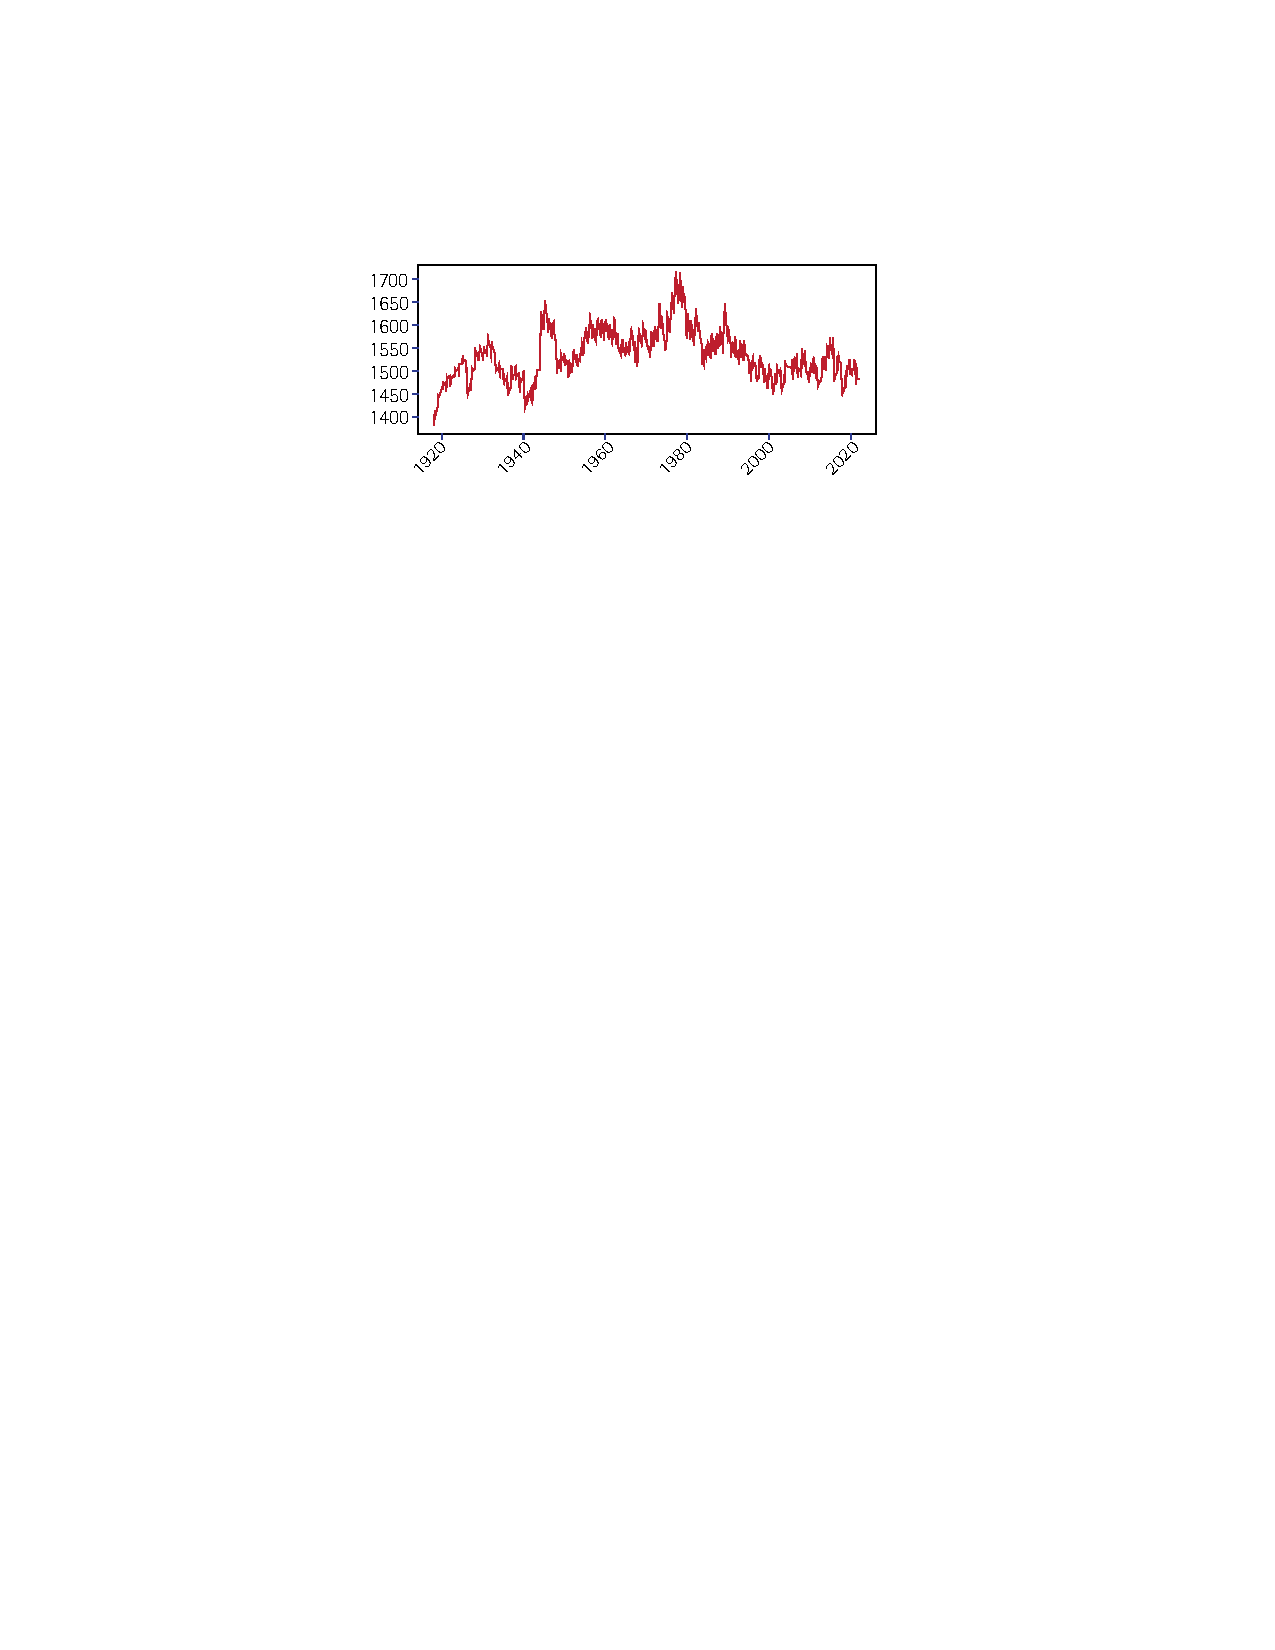
\includegraphics[width= 1\linewidth]{pic3}
		\caption{\small\textit{\color{toanhocdoisong}Hình $2$. Xếp hạng Elo của đội Montreal Canadiens từ năm $1917$ đến nay.}}
		\vspace*{-10pt}
	\end{figure}
	Ngoài ra, mô hình của Best và Paine tính đến cả hiệu số bàn thắng -- bàn thua của mỗi trận đấu và sự phụ thuộc lẫn nhau (hay tự tương quan) giữa các trận đấu liên tiếp.
	\vskip 0.05cm
	Hình $2$ cho thấy sự thay đổi của xếp hạng Elo của đội Montreal Canadiens theo mô hình của Best và Paine. Đỉnh cao nhất của đồ thị nằm ở nửa sau của thập niên $1970$, giai đoạn mà họ giành được bốn cúp Stanley\footnote[5]{\color{toanhocdoisong}Danh hiệu vô địch hàng năm của NHL -- Pi.}  liên tiếp.
	\vskip 0.05cm
	Ta cũng có thể thấy các đỉnh khác trong nửa sau thập niên $1940$ và giữa những năm $1990$, cũng như thời kỳ xuất sắc ổn định cuối những năm $1950$, khi họ vô địch năm lần liên tiếp (từ $1956$ đến $1960$). Trái lại, xếp hạng Elo của đội dao động quanh mức trung bình kể từ đầu những năm $2000$. Sự hiện diện của họ tại trận chung kết cúp Stanley năm $2021$, bởi vậy, có ít khả năng lặp lại trong tương lai gần.
	\begin{figure}[H]
		\vspace*{-10pt}
		\centering
		\captionsetup{labelformat= empty, justification=centering}
		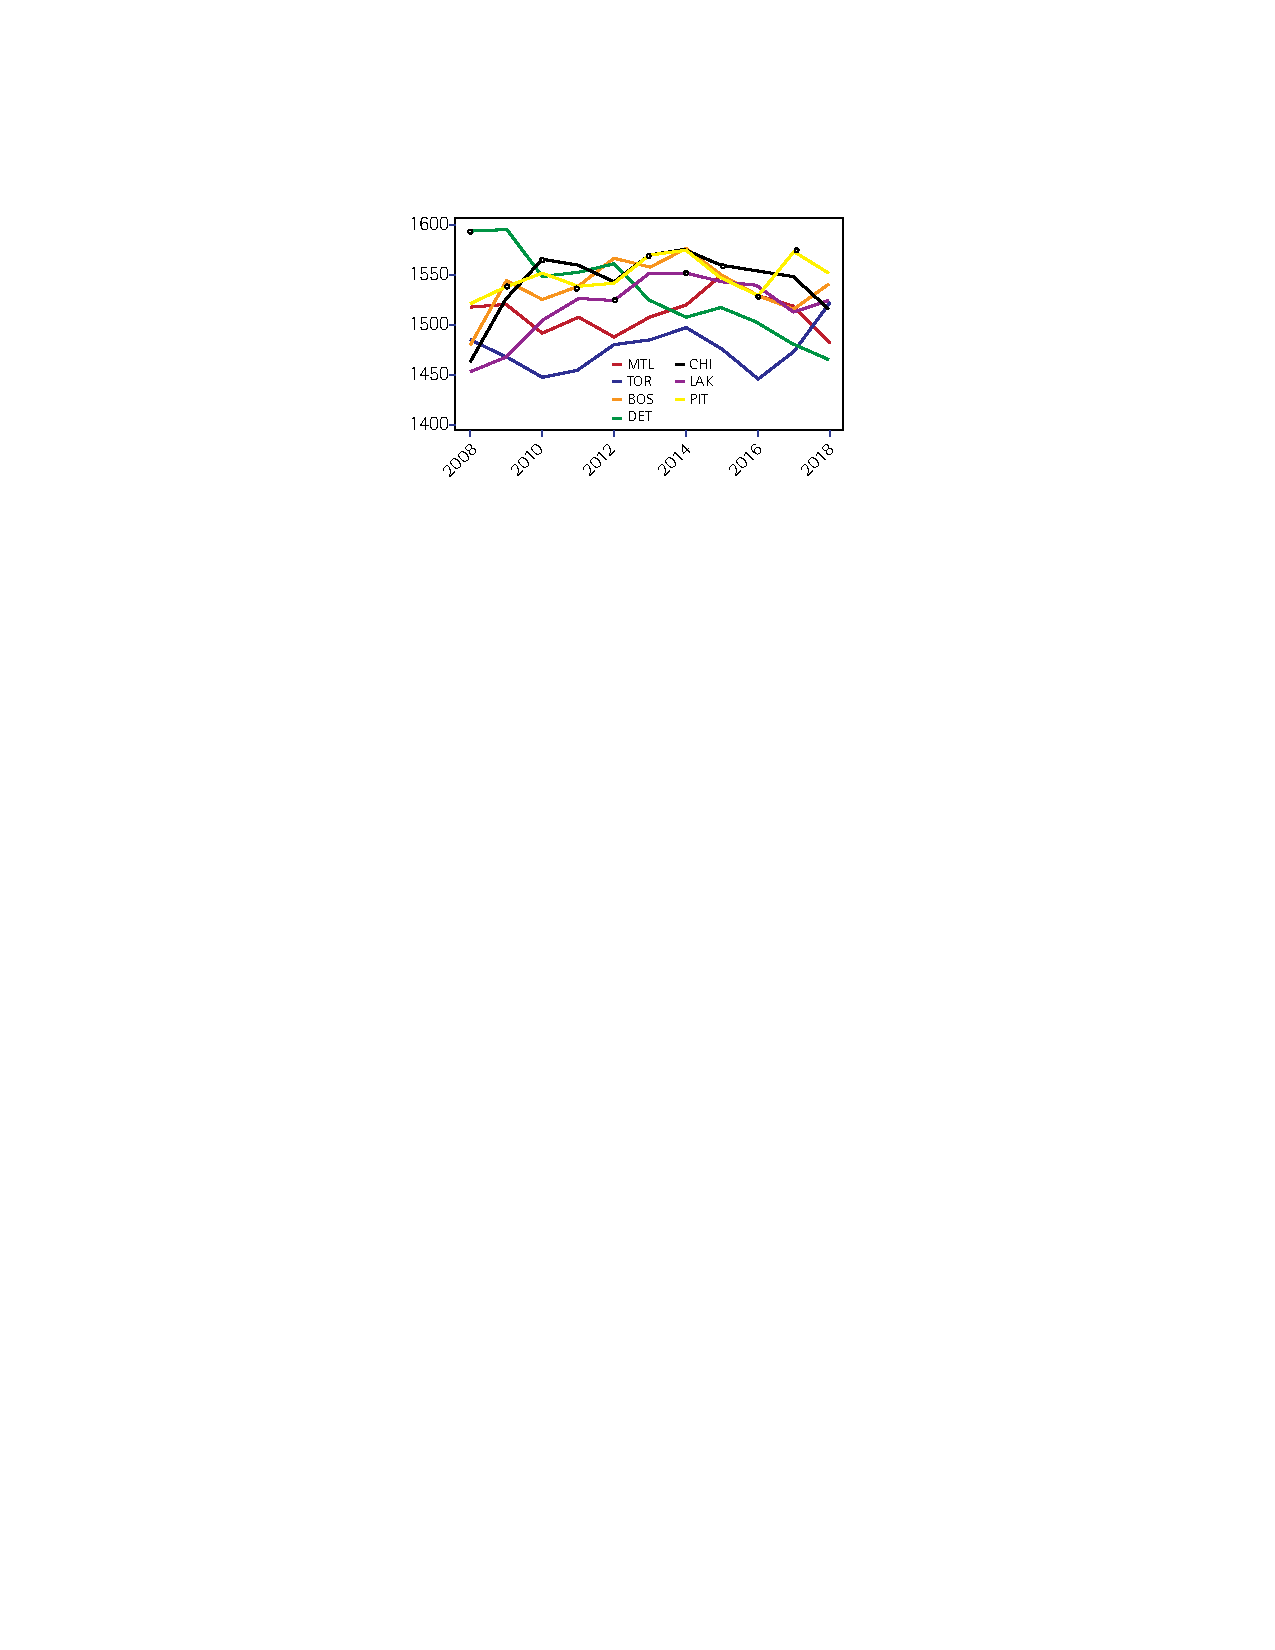
\includegraphics[width= 0.92\linewidth]{pic4}
		\caption{\small\textit{\color{toanhocdoisong}Hình $3$. Xếp hạng Elo của bảy đội NHL từ $2008$ đến $2018$; đội vô địch mỗi năm từ $2008$ đến $2017$ được đánh dấu bằng hình tròn.}}
		\vspace*{-10pt}
	\end{figure}
	Vì xếp hạng Elo có tính tương đối, sẽ bổ ích hơn nếu ta so sánh sự thay đổi xếp hạng của các câu lạc bộ khác nhau. Hình $3$ so sánh các đội Montreal Canadiens (đường màu đỏ), Toronto Maple Leafs (xanh nước biển) và năm đội giành cúp Stanley từ $2008$ đến $2017$, gồm Boston Bruins (da cam), Detroit Red Wings (xanh lá cây), Chicago Blackhawks (đen), Los Angeles Kings (tím) và Pittsburgh Penguins (vàng).
	\vskip 0.05cm
	Trong Hình $3$, các đội vô địch được đánh dấu bằng hình tròn. Đội vô địch năm $2018$, Washington Capitals, không được xét đến trong hình. Có thể thấy rõ là đội hay nhất không phải lúc nào cũng vô địch.
	\vskip 0.05cm
	\textbf{\color{toanhocdoisong}Kết luận}
	\vskip 0.05cm
	Là một yếu tố không thể thiếu trong thế giới cờ vua đồng thời có thể được áp dụng cho các trò chơi hai người có tổng bằng không nói chung, hệ thống tính điểm Elo cho phép đánh giá trình độ tương đối của các đấu thủ ngay cả khi họ chưa từng đối đầu nhau. Sự cập nhật liên tục dần dần qua từng trận đấu đem lại một cách đơn giản và hiệu quả để nắm bắt quá trình thay đổi của các đấu thủ hoặc của các đội, như được minh họa trong thí dụ về NHL.
\end{multicols}
\vspace*{-8pt}
\begin{tBox}
	\begin{wrapfigure}{l}{0.18\linewidth}
		\vspace*{-15pt}
		\centering
		\captionsetup{labelformat= empty, justification=centering}
		\hspace*{3pt}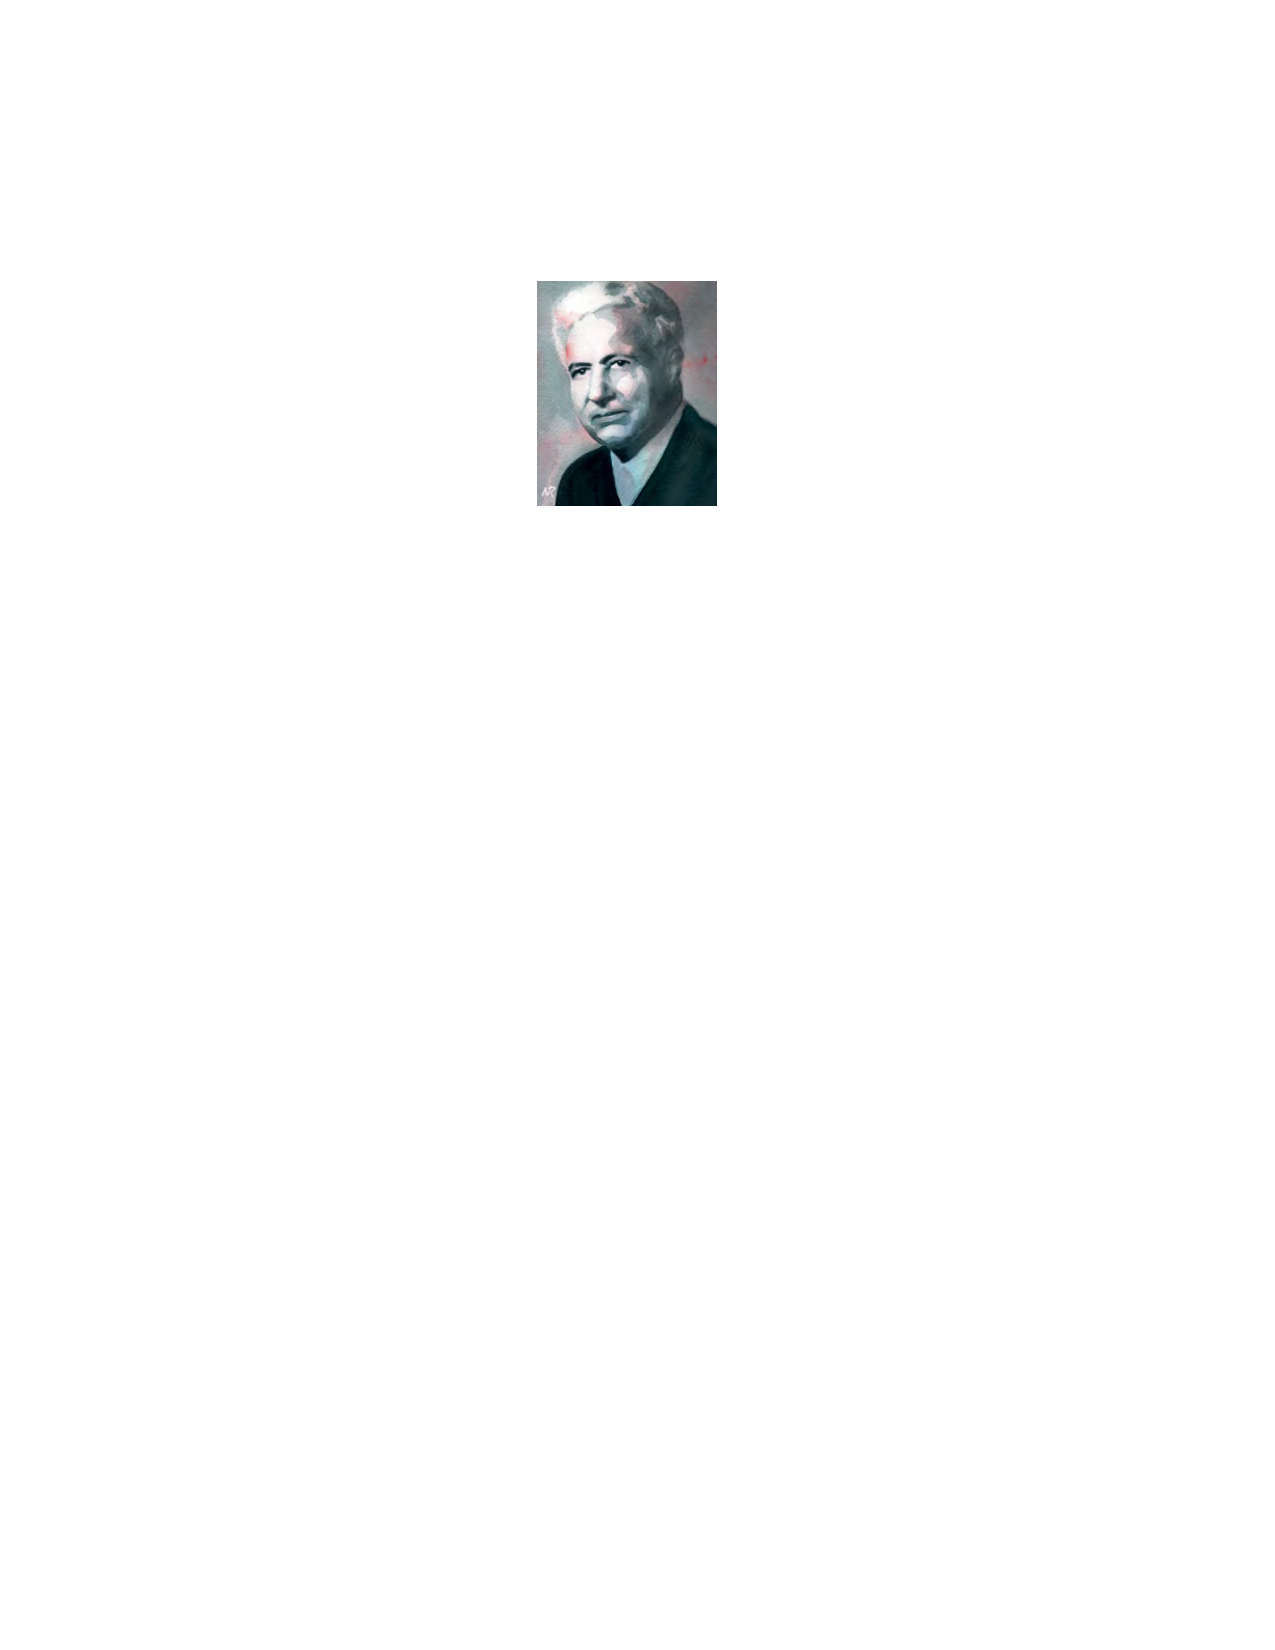
\includegraphics[width= 1.1\linewidth]{pic2}
		\caption{\small\textit{\color{toanhocdoisong}\hspace*{15pt}Arpad Elo.}}
		\vspace*{-20pt}
	\end{wrapfigure}
	Sinh ngày $25$ tháng $8$ năm $1903$ tại Egyházaskeszö, Áo--Hung trong một gia đình khiêm tốn, Arpad Elo (Élö Árpád trong tiếng Hungary) di cư sang Mỹ năm $1913$ cùng cha mẹ. Ông học vật lý tại Đại học Chicago, sau đó giảng dạy tại Đại học Marquette Milwaukee, Wisconsin.
	\vskip 0.05cm
	Ông là một kỳ thủ tài ba, từng tám lần vô địch bang và là chủ tịch Liên đoàn Cờ vua Mỹ từ $1935$ đến $1937$. Ông nổi tiếng thế giới vì đã đưa vào sử dụng hệ thống mang tên mình, được xây dựng trong những năm $1950$ sau khi hệ thống xếp hạng đầu tiên, do Kenneth Harkness phát triển, bị chỉ ra những nhược điểm. Phương pháp mới được FIDE thông qua vào năm $1970$, và Elo trở thành thành viên danh dự của tổ chức này từ năm $1981$.
	\vskip 0.05cm
	Một phân tích chi tiết đầu tiên về hệ thống tính điểm Elo (có khi bị viết sai thành ELO như thể một từ viết tắt) được chính Elo đưa ra trong cuốn sách năm $1978$ của mình, The Rating of Chessplayers, Past and Present. Ngày nay, phương pháp của ông là một phần không thể tách rời của thế giới cờ vua. Nó được dùng để xác định cách các kỳ thủ đối đầu với nhau tại các giải cờ vua trên toàn thế giới, và mọi kỳ thủ đều theo dõi sát sao sự thay đổi điểm số Elo của mình để đo mức độ tiến bộ và biết được thứ bậc của mình trong cờ vua.
	\vskip 0.05cm
	Arpad Elo qua đời ngày $5$ tháng $11$ năm $1992$ (thọ $89$ tuổi) tại Brookfield, Wisconsin.
	\vspace*{-5pt}
\end{tBox}
	\newpage
	
	\setcounter{figure}{0}
	\thispagestyle{duongvaotoanhocnone}
\pagestyle{duongvaotoanhoc}
\everymath{\color{duongvaotoanhoc}}
\graphicspath{{../duongvaotoanhoc/pic/}}
\blfootnote{$^1$\color{duongvaotoanhoc}Viện Toán học.}
\begingroup
\AddToShipoutPicture*{\put(0,616){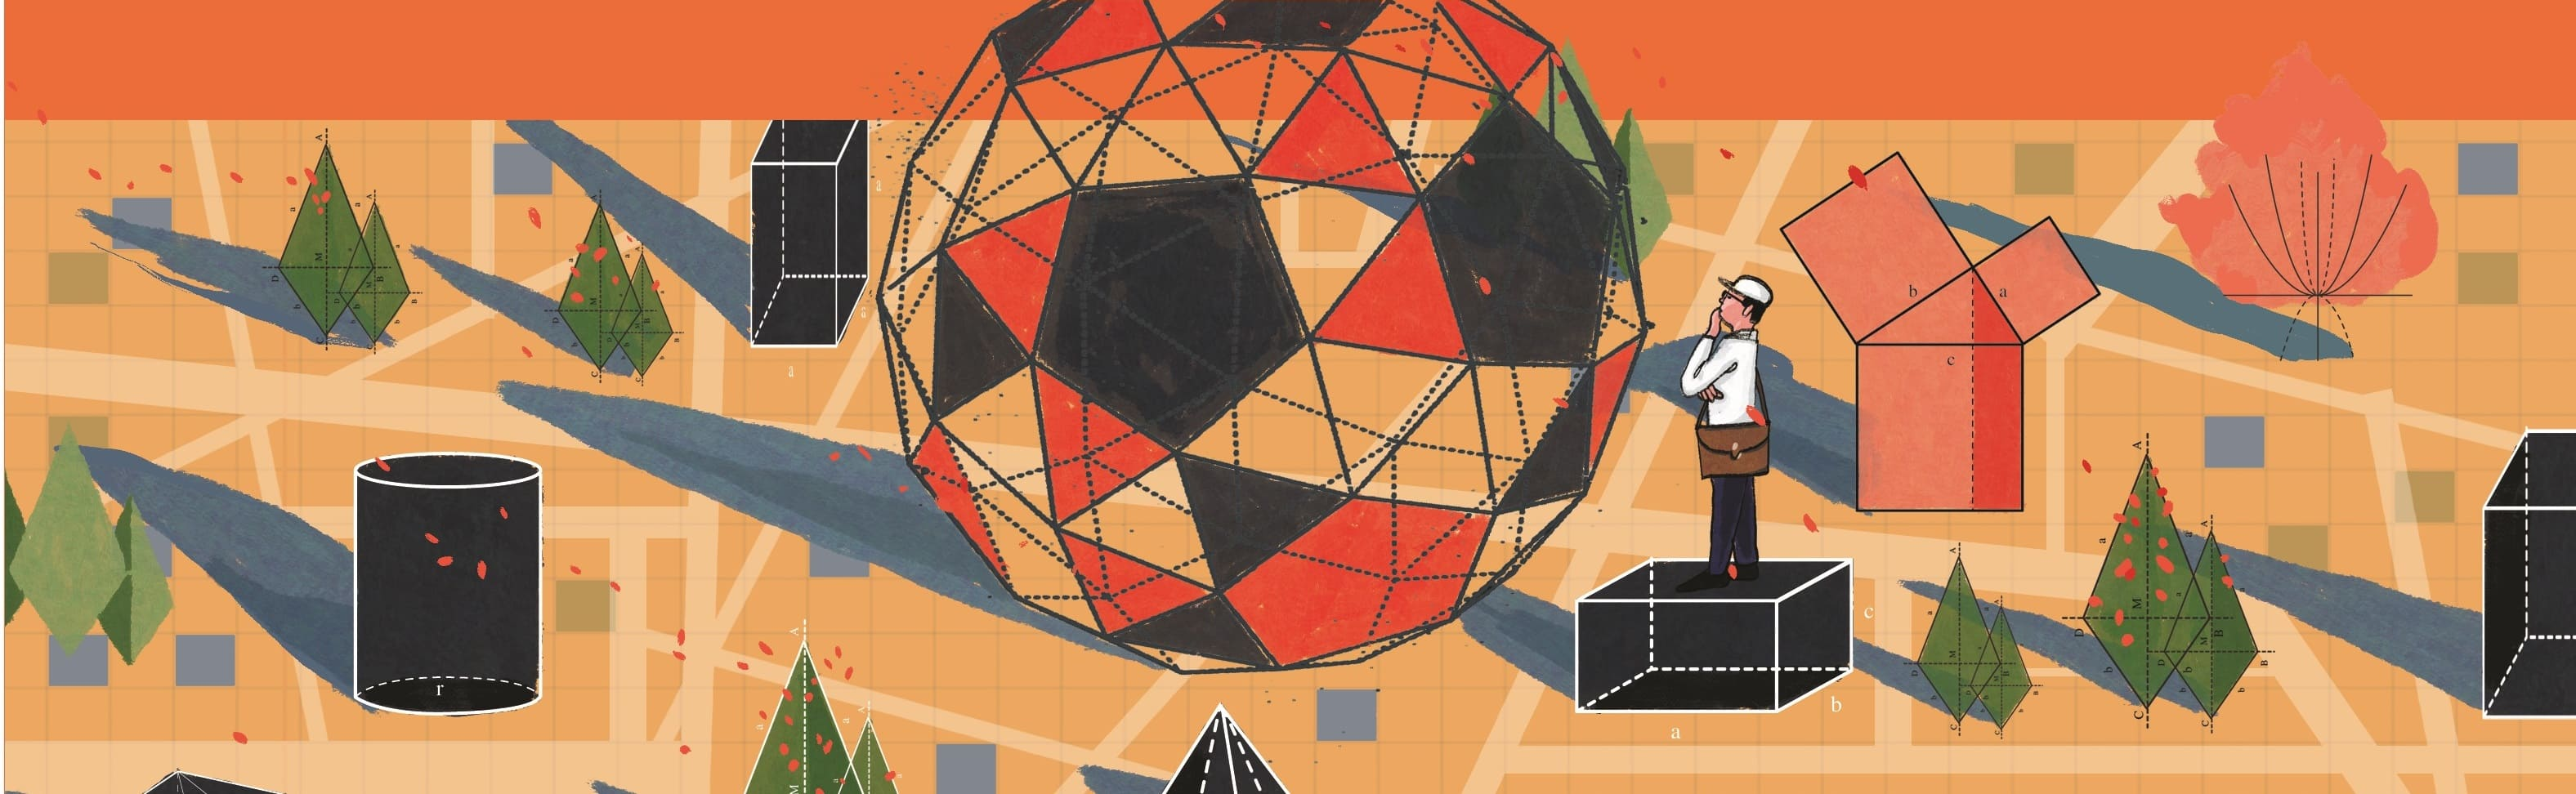
\includegraphics[width=19.3cm]{../bannerduongvao}}}
\AddToShipoutPicture*{\put(168,553){
\includegraphics[scale=1]{../tieude.pdf}}}
\centering
\endgroup
\vspace*{154pt}

\begin{multicols}{2}	
	Chúng ta biết rằng một đa thức hệ bậc $n\geq 1$ với hệ số thực có không quá $n$ nghiệm thực. Điều này cũng có thể được minh họa là đồ thị của nó cắt trục hoành tại không quá $n$ điểm. Tổng quát hơn ta có: đồ thi  đó cắt một đường thẳng bất kỳ cũng tại không quá $n$ điểm. 
	\begin{figure}[H]
		\centering
		\vspace*{-5pt}
		\captionsetup{labelformat= empty, justification=centering}
		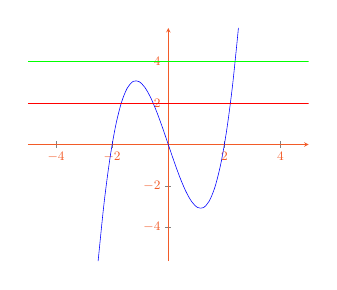
\begin{tikzpicture}[scale=0.52, duongvaotoanhoc, node font= \small]
			\begin{axis} [axis lines=center]
				\addplot [blue,domain=-2.5:2.5, smooth] { x^3 - 4*x };
				\addplot [domain=-5:5,red,smooth] {2};
				\addplot [domain=-5:5,green,smooth] {4};
			\end{axis}
		\end{tikzpicture}
		\caption{\small\textit{\color{duongvaotoanhoc}Hình $1$.}}
		\vspace*{-10pt}
	\end{figure}
	Nếu cho hai đường elipse trên mặt phẳng cắt nhau ta thấy số giao điểm không thể quá $4$. Điều này cũng đúng với các đường parabola và hyperbola.
	\vskip 0.1cm
	Nếu cho một elipse cắt đồ thị của một đa thức bậc $3$ thì số giao điểm có thể lên tới $6$. Ta thấy, số giao điểm lớn nhất có thể liên quan tới bậc của các đường cong mà ta đang xét.
	\begin{figure}[H]
		\centering
		\vspace*{-5pt}
		\captionsetup{labelformat= empty, justification=centering}
		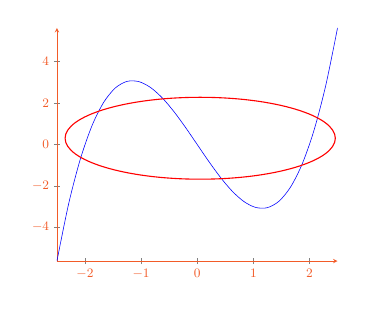
\begin{tikzpicture}[duongvaotoanhoc,scale=0.52, node font= \small]
			\begin{axis}[domain=-5:5, axis x line=bottom,axis y line=left]
				\addplot [blue,domain=-2.5:2.5, smooth] { x^3 - 4*x };
			\end{axis}
			\draw[red] (3.5,3) ellipse (3.3cm and 1cm);
		\end{tikzpicture}
		\caption{\small\textit{\color{duongvaotoanhoc}Hình $2$.}}
		\vspace*{-5pt}
	\end{figure}
	Nếu xét đa thức hệ số phức và các nghiệm phức, đồng thời tính cả bội thì một đa thức bậc $n\geq 1$ với hệ số phức có đúng $n$ nghiệm. Ta cũng có thể nói, ``đồ thị'' của đa thức này cắt ``đường thẳng phức'' tại đúng $n$ điểm nếu tính cả bội.
	\vskip 0.1cm
	Định lý Bézout phát biểu rằng {\em hai đường cong đại số trên mặt phẳng xạ ảnh cắt nhau tại đúng $n$ điểm nếu kể cả bội, với $n$ là tích của bậc của hai đường cong} (ngoại trừ trường hợp chúng trùng nhau một phần). 
	\vskip 0.1cm
	Khẳng định về số giao điểm của hai đường cong trên mặt phẳng đã được phát biểu nhiều lần trong nhiều tác phẩm bởi các nhà toán học nổi tiếng như Newton ($1665$), Maclaurin ($1720$), Euler và Cramber ($1748$). Tuy nhiên trước Etienne Bézout ($1730-1783$), chưa có một chứng minh cụ thể nào được đưa ra. 
	\vskip 0.1cm
	Bézout đưa ra chứng minh năm $1779$ trong cuốn sách {\em Théorie générale des équations algébraiques} (Lý thuyết đại cương về phương trình đại số). Một đường cong đại số trên mặt phẳng được xác định như tập nghiệm của một đa thức hai biến. Như vậy khẳng định có thể được phát biểu như là số nghiệm của một hệ hai phương trình đa thức theo hai ẩn.
	Bézout đã đưa ra khái niệm {\em kết thức} để giải quyết bài toán. Cho hai đa thức $F(x)$ và $G(x)$ hệ số phức với bậc tương ứng là $m$ và $n$. Ký hiệu $\mathbb C[x]_d$ là không gian véc tơ các đa thức với bậc nhỏ hơn $d$. Xét ánh xạ tuyến tính ``Bézout'' cho bởi 
%	\setlength{\abovedisplayskip}{5pt}
%	\setlength{\belowdisplayskip}{5pt}
	\begin{align*}
		\mathbb C[x]_n\!\times\! \mathbb C[x]_m \!\rightarrow\!  \mathbb C[x]_{m\!+\!n},
		(A,B)\!\mapsto\! AF\!+\!BG.
	\end{align*}
	Nhận xét là số chiều của hai không gian nguồn và đích cùng bằng $m+n$. Do đó ta có thể xét định thức của ánh xạ này. Đây chính là kết thức của $F$ và $G$. Theo bổ đề Bézout (xem Bổ đề $2$ dưới đây), nếu $F$ và $G$ có nghiệm chung thì ánh xạ trên có hạch không tầm thường, từ đó kết thức bằng $0$, và ngược lại. 
	\vskip 0.1cm
	Bằng cách coi hai đa thức theo $x$ và $y$ như là các đa thức theo biến $y$, thì kết thức của chúng sẽ là một đa thức theo $x$ với bậc không vượt quá tích các bậc của hai đa thức ban đầu. Từ đó Bézout có một chứng minh cho các đa thức (và do đó các đường cong) ở vị trí tổng quát. 
	\vskip 0.1cm
	Một chứng minh chặt chẽ và bao quát hết mọi khả năng chỉ được đưa ra bởi Georges--Henri Halphen năm $1873$. 
	Khó khăn trong việc phát biểu và chứng minh dạng tổng quát của định lý Bézout là việc định nghĩa khái niệm bội của giao điểm của hai đường cong đại số. J.--P. Serre ($1965$) đề xuất giải quyết vấn đề này một cách triệt để thông qua vành địa phương. Đây cũng có thể coi là một trong những điểm xuất phát của Hình học Đại số hiện đại. 
	\vskip 0.1cm
	$\pmb{1.}$ \textbf{\color{duongvaotoanhoc}Đường cong cho bởi phương trình đa thức}
	\vskip 0.1cm
	Một đường thẳng trong mặt phẳng được xác định bởi phương trình  
	\begin{align*}
		ax+by+c=0
	\end{align*}
	trong đó ít nhất một trong hai số $a$ hoặc $b$ khác $0$. Tương tự, một đường cong bậc $2$, còn gọi là đường conic, được xác định bởi phương trình
	\begin{align*}
		ax^2+bxy+cx^2+dx+ey+g=0,
	\end{align*}
	với ít nhất một trong các hệ số $a,b,c$ khác $0$.
	\vskip 0.1cm
	Tổng quát, một {\em đường cong đại số} trên mặt phẳng (còn gọi tắt là đường cong phẳng) được định nghĩa như là tập nghiệm của một đa thức hai biến (khác hằng số):
	\begin{align*}
		F(x,y)=0. \tag{$1$}
	\end{align*}
	Ở đây $F$ là một đa thức theo hai biến $x$ và $y$:
	\begin{align*}
		F(x,y)=\sum_{i,j} a_{ij}x^iy^j,
	\end{align*}
	trong đó tổng ở vế phải là một tổng hữu hạn. Tổng lớn nhất các số mũ trong các đơn thức $x^iy^j$ ở vế phải được gọi là {\em bậc} của $F$, ký hiệu $\deg F$. 
	\vskip 0.1cm
	Xét {\em họ các đường cong} xác định bởi phương trình
	\begin{align*}
		(ax+by+c)^2-\alpha=0,
	\end{align*}
	với $\alpha$ thay đổi. Khi $\alpha\neq 0$ phương trình này xác định một cặp hai đường thẳng song song. Khi $\alpha$ tiến tới $0$, hai đường thẳng này tiến gần tới nhau và khi $\alpha=0$, hai đường thẳng này tạo thành {\em một đường thẳng kép}. 
	\vskip 0.1cm
	Như vậy hình ảnh hình học của tập nghiệm không phản ánh hết bản chất đại số của phương trình, đặc biệt khi phương trình đó phụ thuộc vào tham số. Để giải quyết vấn đề này, ta sẽ sử dụng {\em ngôn ngữ đại số} để mô tả hình học. Định nghĩa của một đường cong đại số vì thế sẽ được phát biểu như sau. 
	\vskip 0.2cm
	\PIbox{\em Đường cong đại số trong mặt phẳng được xác định bởi một đa thức $F\in \mathbb C[x,y]$ có bậc lớn hơn hoặc bằng 1, tập các điểm hình học của nó là nghiệm của phương trình $F$. Đường cong đại số này được gọi tắt là {\em đường cong $F$}. }
	\vskip 0.2cm
	Trong Hình học Đại số, thay vì xét các tập nghiệm thực của phương trình ($1$), người ta xét các nghiệm phức. Có một số khác biệt căn bản giữa nghiệm thực và nghiệm phức, từ góc độ đại số cũng như từ góc độ hình học. 
	\vskip 0.1cm
	($1$) Một trong những tính chất đại số quan trọng nhất của số phức là mọi đa thức hệ số phức với bậc $n\geq 1$ đều có đủ $n$ nghiệm phức, nếu tính cả bội.   
	\vskip 0.1cm 
	($2$) Từ góc độ hình học chúng ta biết rằng tập các số phức lập thành một mặt phẳng, thường gọi là {\em mặt phẳng phức}. Do đó tập các số phức có chiều hình học bằng $2$. Như vậy, một đường cong phức cũng có số chiều bằng $2$. 
	\vskip 0.1cm
	($3$) Để phân biệt mặt phẳng phức với không gian tuyến tính phức hai chiều ta sẽ gọi không gian này là {\em mặt phẳng affine phức}. Chữ ``affine'' hàm ý ta chỉ xét nó như một không gian tuyến tính và chỉ quan tâm tới các tính chất song song hay cắt nhau của các đường thẳng, hoặc tính thẳng hàng hay không thẳng hàng của các điểm, mà không quan tâm tới các yếu tố như góc hay khoảng cách. 
	\vskip 0.1cm
	($4$) Việc hình dung hình học các đường cong đại số phức tương đối khó. Ví dụ hai đường thẳng phức trong không gian phức hai chiều thường cắt nhau tại duy nhất một điểm. Nhìn từ góc độ hình học điều đó có nghĩa là hai mặt phẳng trong không gian bốn chiều cắt nhau tại một điểm. 
	\vskip 0.1cm
	($5$) Do đó, để thuận tiện cho tư duy hình học, đôi khi ta sử dụng ``phần thực'' của một đường cong phức, khi nó được xác định như là tập nghiệm của một đa thức hệ số thực. Tuy nhiên chúng ta cần cảnh giác rằng nhiều kết luận đúng đối với phần thực, có thể không đúng đối với toàn bộ đường cong phức. 
	\vskip 0.1cm
	Ví dụ xét tập nghiệm của phương trình
	\begin{align*}
		xy-1=0.
	\end{align*}
	Đây là một hyperbola. Phần thực của nó bao gồm hai nhánh rời nhau. 
	Thực hiện một phép đổi biến với hệ số phức:
	$x'=(x+y)/2;\ y'=(x-y)/2i$, ta có
	\begin{align*}
		{x'}^2+{y'}^2=xy=1.
	\end{align*}
	Nghĩa là nếu ``cắt'' đường cong phức $xy-1=0$ bởi mặt phẳng thực căng trên hai véc tơ $x'$ và $y'$ thì ta thu được một đường tròn. 
	\vskip 0.1cm
	Thực tế, toàn bộ đường cong là một mặt hai chiều liên thông! 
	Để thấy rõ hơn điều này ta biểu diễn các biến phức $x$ và $y$ theo các biến thực:
	\begin{align*}
		x=u+iv\text{ và } y=w+iz.
	\end{align*}
	Phương trình trên được đưa về dạng:
	\begin{align*}
		\begin{cases}
			 uw-vz=1\\
			 uz+vw=0.
		\end{cases}
	\end{align*}
	Từ đó ta suy ra
	\begin{align*}
		t:=\frac uw=-\frac vz\neq 0.
	\end{align*}
	Thế vào phương trình đầu ta thu được
	\begin{align*}
		u^2+v^2=t.
	\end{align*}
	\begin{figure}[H]
		\vspace*{-5pt}
		\centering
		\captionsetup{labelformat= empty, justification=centering}
		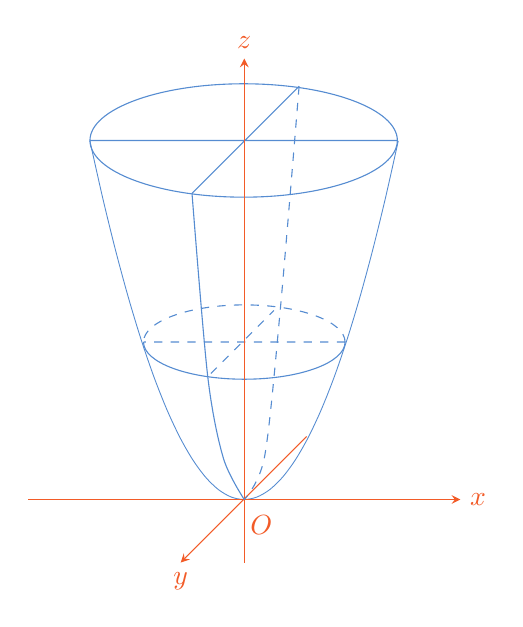
\begin{tikzpicture}[duongvaotoanhoc,scale=0.8]
			\begin{axis}[axis lines = center, xmin=-3.5,xmax=3.5, ticks = none, axis line style={draw=none}]
				\addplot [cackithi,domain=-2.5:2.5, smooth] {x^2};
			\end{axis}
			\draw[dashed, cackithi] (5.03,2.5) arc
			[
			start angle=0,
			end angle=180,
			x radius=1.6cm,
			y radius =0.59cm
			];
			\draw[cackithi] (5.03,2.5) arc
			[
			start angle=0,
			end angle=-180,
			x radius=1.6cm,
			y radius =0.59cm
			];
			\draw[cackithi] (5.86,5.7) arc
			[
			start angle=0,
			end angle=360,
			x radius=2.44cm,
			y radius =0.9cm
			];
			\draw[cackithi] (5.86,5.7) -- (0.98,5.7) (2.6,4.86) -- (4.3,6.56);
			\draw[cackithi, dashed] (5.03,2.5) -- (1.83,2.5) (2.9,2) -- (3.9,3);
			\draw[-stealth] (4.42,1) -- (2.42,-1) node [below] {$y$};
			\draw[-stealth] (0,0) -- (6.86, 0) node [right] {$x$};
			\draw[-stealth] (3.43,-1) -- (3.43, 7) node [above] {$z$};
			\draw[cackithi] plot [smooth] coordinates {(2.6,4.86) (2.85,1.95) (3.1,0.65) (3.43,0)};
			\draw[cackithi, dashed] plot [smooth] coordinates {(4.3,6.56) (4,3) (3.75,0.67) (3.43,0)};
			\draw (3.7, -0.4) node {$O$};
		\end{tikzpicture}
		\caption{\small\textit{\color{duongvaotoanhoc}Hình $3$.}}
		\vspace*{-10pt}
	\end{figure}
	Như vậy:
	\vskip 0.2cm
	\PIbox{trong không gian $3$ chiều với các tọa độ là $u,v,t$, nghiệm của phương trình xác định {\bf\color{duongvaotoanhoc} đường hyperbola phức} lập thành một {\bf\color{duongvaotoanhoc} mặt paraboloid tròn xoay thực}, bỏ đi điểm $(0,0,0)$ (ứng với giá trị $t=0$).}
	\vskip 0.2cm
	$\pmb{2.}$ \textbf{\color{duongvaotoanhoc}Đường cong  bất khả quy}
	\vskip 0.1cm 
	Nếu đa thức $F$ phân tích thành hai đa thức $G$ và $H$, bậc $>0$, thì tập nghiệm của $F=$ là hợp các tập nghiệm của $G=0$ và $H=0$. Một đa thức được gọi là {\em bất khả quy} nếu nó không có phân tích như trên. Đường cong xác định bởi đa thức này cũng được gọi là {\em bất khả quy}. Kết quả sau đây khẳng định rằng một đường cong đại số sẽ là hợp của các đường cong bất khả quy.
	\vskip 0.1cm
	\textbf{\color{duongvaotoanhoc}Định lý} $\pmb{1.}$ \textit{Một đa thức hai biến với hệ số phức luôn phân tích được theo một cách duy nhất (sai khác các hệ số khác 0) thành tích các đa thức bất khả quy.}
	\vskip 0.1cm 
	Phân tích đa thức $F$ ra các thành phần bất khả quy:
	\begin{align*}
		F =\prod_{i=1}^r F_i{}^{d_i},\quad d_i\geq 1.
	\end{align*}
	Khi đó đường cong $F$  là hợp của các đường cong $F_i$. Ta cũng nói mỗi đường cong  $F_i$ là một {\em thành phần bất khả quy} của đường cong  $F$. Số $d_i$ được gọi là số bội của thành phần bất khả quy tương ứng. 
	\vskip 0.1cm
	Chứng minh của định lý $1$ là mẫu mực cho cách tiếp cận sơ cấp tới các đa thức nhiều biến. Ý tưởng cơ bản là đưa việc xét đa thức theo hai biến $x,y$ về việc xét các đa thức theo biến $x$ với hệ số là các đa thức theo biến $y$, sau đó ta mở rộng tập các hệ số ra các phân thức đại số theo $y$. Phương pháp này tương tự như khi ta sử dụng các đa thức với hệ số hữu tỷ để giải quyết bài toán cho các đa thức hệ số nguyên. 
	\vskip 0.1cm
	Các bạn học sinh giỏi toán bậc THPT rất nên thử tìm cách chứng minh định lý trên. Ý tưởng chứng minh sử dụng bổ đề quen thuộc của Bézout và  Gauss cho đa thức hai biến. 
	\vskip 0.1cm
	Dưới đây là phát biểu của các bổ đề này cho các đa thức hệ số nguyên. 
	\vskip 0.1cm
	\textbf{\color{duongvaotoanhoc}Bổ đề} $\pmb{2}$ (Bézout)\textbf{\color{duongvaotoanhoc}.} \textit{Cho hai số nguyên $m$ và $n$. Khi đó tồn tại các số nguyên $k$ và $l$ sao cho }
		\begin{align*}
			k\cdot m+l\cdot n=\textrm{\rm UCLN}(m,n).
		\end{align*}
	\vskip 0.1cm
	\textbf{\color{duongvaotoanhoc}Bổ đề} $\pmb{3}$ (Gauss)\textbf{\color{duongvaotoanhoc}.}
	\textit{Đối với một đa thức $P(x)$ với hệ số nguyên ta định nghĩa {\em  dung lượng} của $P(x)$ là ước chung lớn nhất của các hệ số của $P(x)$, ký hiệu là $c(P)$. Đa thức $P(x)$ được gọi là {\em rút gọn} nếu $c(P)=1$. Với hai đa thức hệ số nguyên tùy ý $P(x)$, $Q(x)$ ta luôn có}
	\begin{align*}
		c(P\cdot Q)=c(P)\cdot c(Q).
	\end{align*}
	Vành đa thức $\mathbb C[x]$ có nhiều tính chất số học giống vành các số nguyên. Cụ thể, trong đó cũng có thể thực hiện được phép chia có dư. Tập các phân thức hữu tỷ $\mathbb C(x)$ đóng vai trò tương tự như tập các số hữu tỷ. 
	Việc phát biểu và chứng minh các kết quả tương tự với bổ đề Gauss và Bézout cho các đa thức hai biến dành cho bạn đọc.  
	\vskip 0.1cm	
	$\pmb{3.}$ \textbf{\color{duongvaotoanhoc}Điểm đơn và tiếp tuyến}
	\vskip 0.1cm
	Tiếp tuyến tới đồ thị của đa thức $P(x)$ tại điểm $x=a$, $y=P(a)$ được cho bởi phương trình
	\begin{align*}
		y-P(a)=P'(a)(x-a).
	\end{align*}
	Ta có thể mở rộng kết quả này cho một đường cong đại số bất kỳ cho bởi đa thức $F(x,y)$. Giả sử $P(a,b)$ là một điểm trên đường cong (nghĩa là $F(a,b)=0$). Nếu một trong hai đạo hàm riêng 
	\begin{align*}
		F_x:=\frac{\partial F}{\partial x} \textrm{ hoặc } F_y:=\frac{\partial F}{\partial y}
	\end{align*}
	khác $0$ tại $P$ thì tiếp tuyến tại $P$ tới đường cong được cho bởi phương trình:
	\begin{align*}
		F_x(a,b)(x-a)+F_y(a,b) (y-b)=0. \tag{$2$}
	\end{align*}
	Có nhiều cách để lý giải điều này. Cách đơn giản nhất là thông qua khai triển Taylor đối với $F$ tại điểm $P(a,b)$. Do $F(a,b)=0$ nên khai triển này có dạng:
	\begin{align*}
		F(x,y)=&F_1(x-a,y-b)\\
		&+F_2(x-a,y-b)+\ldots,
	\end{align*}
	trong đó $F_1(x-a,y-b)= F_x(a,b)(x-a)+F_y(a,b)(y-b)$, còn các số hạng $F_2(x-a,y-b)$... có bậc cao hơn theo $x-a$ và $y-b$.  Do tiếp tuyến tới một đường cong tại một điểm $P$ trên đường cong mô tả \textit{xấp xỉ tuyến tính} của phần đường cong tại xung quanh điểm $P$, ta kết luận, phương trình của tiếp tuyến được cho bởi công thức ($2$).
	\vskip 0.1cm
	Nhận xét rằng khai triển Taylor của một đa thức thực ra chính là sắp xếp các đơn thức theo lũy thừa tăng dần, sau khi đã đổi biến đưa điểm đang xét về gốc tọa độ: $(x,y)\mapsto (x-a,y-b)$. 
	\vskip 0.1cm
	\PIbox{Một điểm trên đường cong $F$ được gọi là \textbf{\color{duongvaotoanhoc}điểm đơn} nếu ít nhất một đạo hàm riêng của $F$ tại điểm đó khác $0$.  }
	\vskip 0.1cm
	\textbf{\color{duongvaotoanhoc}Ví dụ.} Khai triển Taylor của đa thức 
	$F(x,y)=x^2+y^2$ 
	tại điểm $A(1,2)$ được cho bởi
	\begin{align*}
		F(x,y)=\,&((x-1)+1)^2+((y-2)+2)^2\\
		=\,&F(1,2)+[2(x-1)+4(y-2)]\\
		&+[(x-1)^2+(y-2)^2].
	\end{align*}
	Do điểm $A(1,2)$ nằm trên đường cong $F-5=0$ nên tiếp tuyến tại đó được cho bởi phương trình
	\begin{align*}
		2(x-1)+4(y-2)=0.
	\end{align*}
	$\pmb{4.}$ \textbf{\color{duongvaotoanhoc}Điểm bội và tiếp tuyến}
	\vskip 0.1cm 
	Một điểm trên đường cong $F$  được gọi là điểm bội nếu nó không phải là điểm đơn. Trước tiên ta sẽ xét trường hợp $F$ là một đa thức bất khả quy trong $\mathbb C[x,y]$. Để đơn giản ta sẽ giả thiết điểm đang xét là gốc tọa độ $O(0,0)$. Các hình vẽ dưới đây mô tả ``phần thực'' của một số đường cong tại lân cận điểm $O$:
	\vskip 0.1cm
	Nhắc lại rằng nếu điểm $O(0,0)$ là điểm bội của $F(x,y)$ khai triển Taylor của $F$ tại $O$ có dạng
	\begin{align*}
		F=F_m+F_{m+1}+\ldots, \quad m\geq 2,
	\end{align*}
	trong đó $F_i$ là các đa thức thuần nhất bậc $i$ theo $x$ và $y$. 
	\begin{figure}[H]
		\vspace*{-10pt}
		\centering
		\captionsetup{labelformat= empty, justification=centering}
		
\includegraphics[height=0.4\linewidth]{4a}\quad\quad
		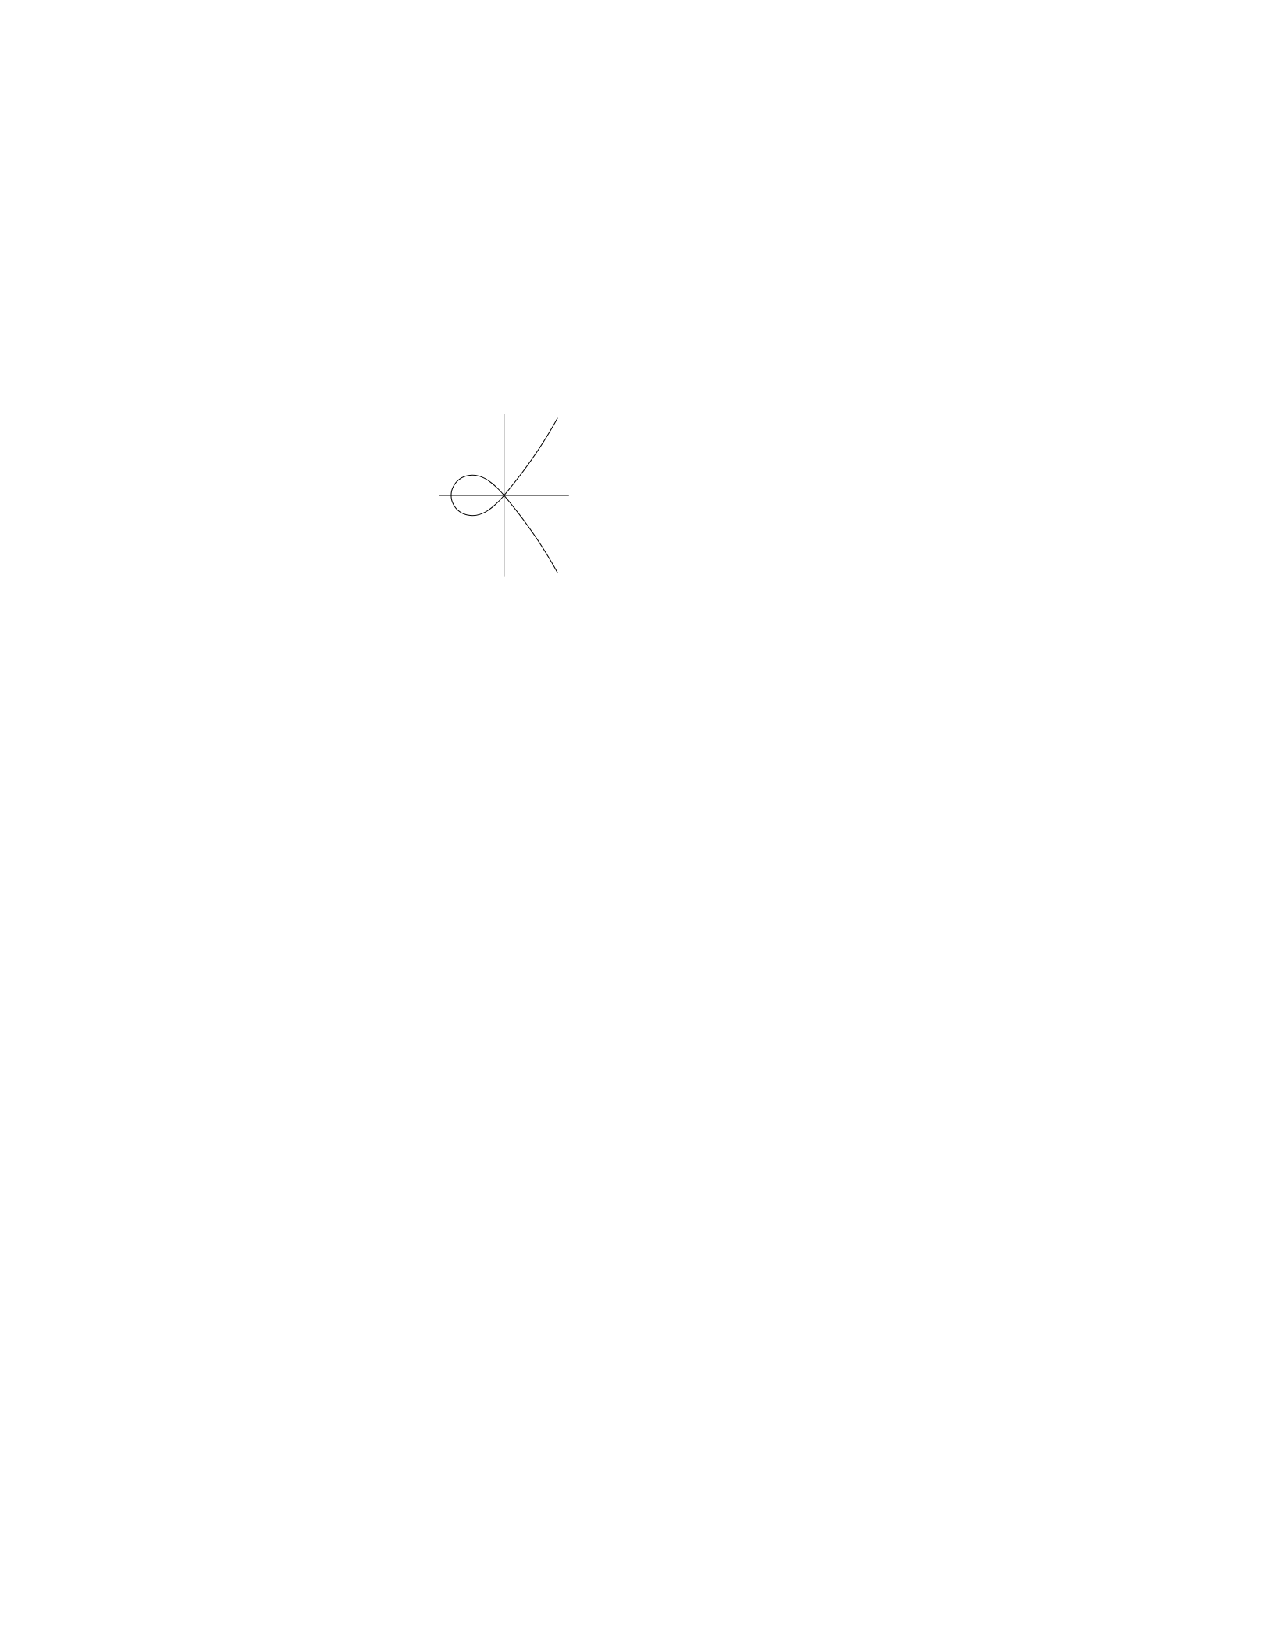
\includegraphics[height=0.4\linewidth]{4b}
		\caption{\small\quad\quad$F=x^3-y^2$ \quad\quad$F\!=\!(x^2 \!+\! y^2)^2 \!+\! 3x^2y\!-\!y^3$}
		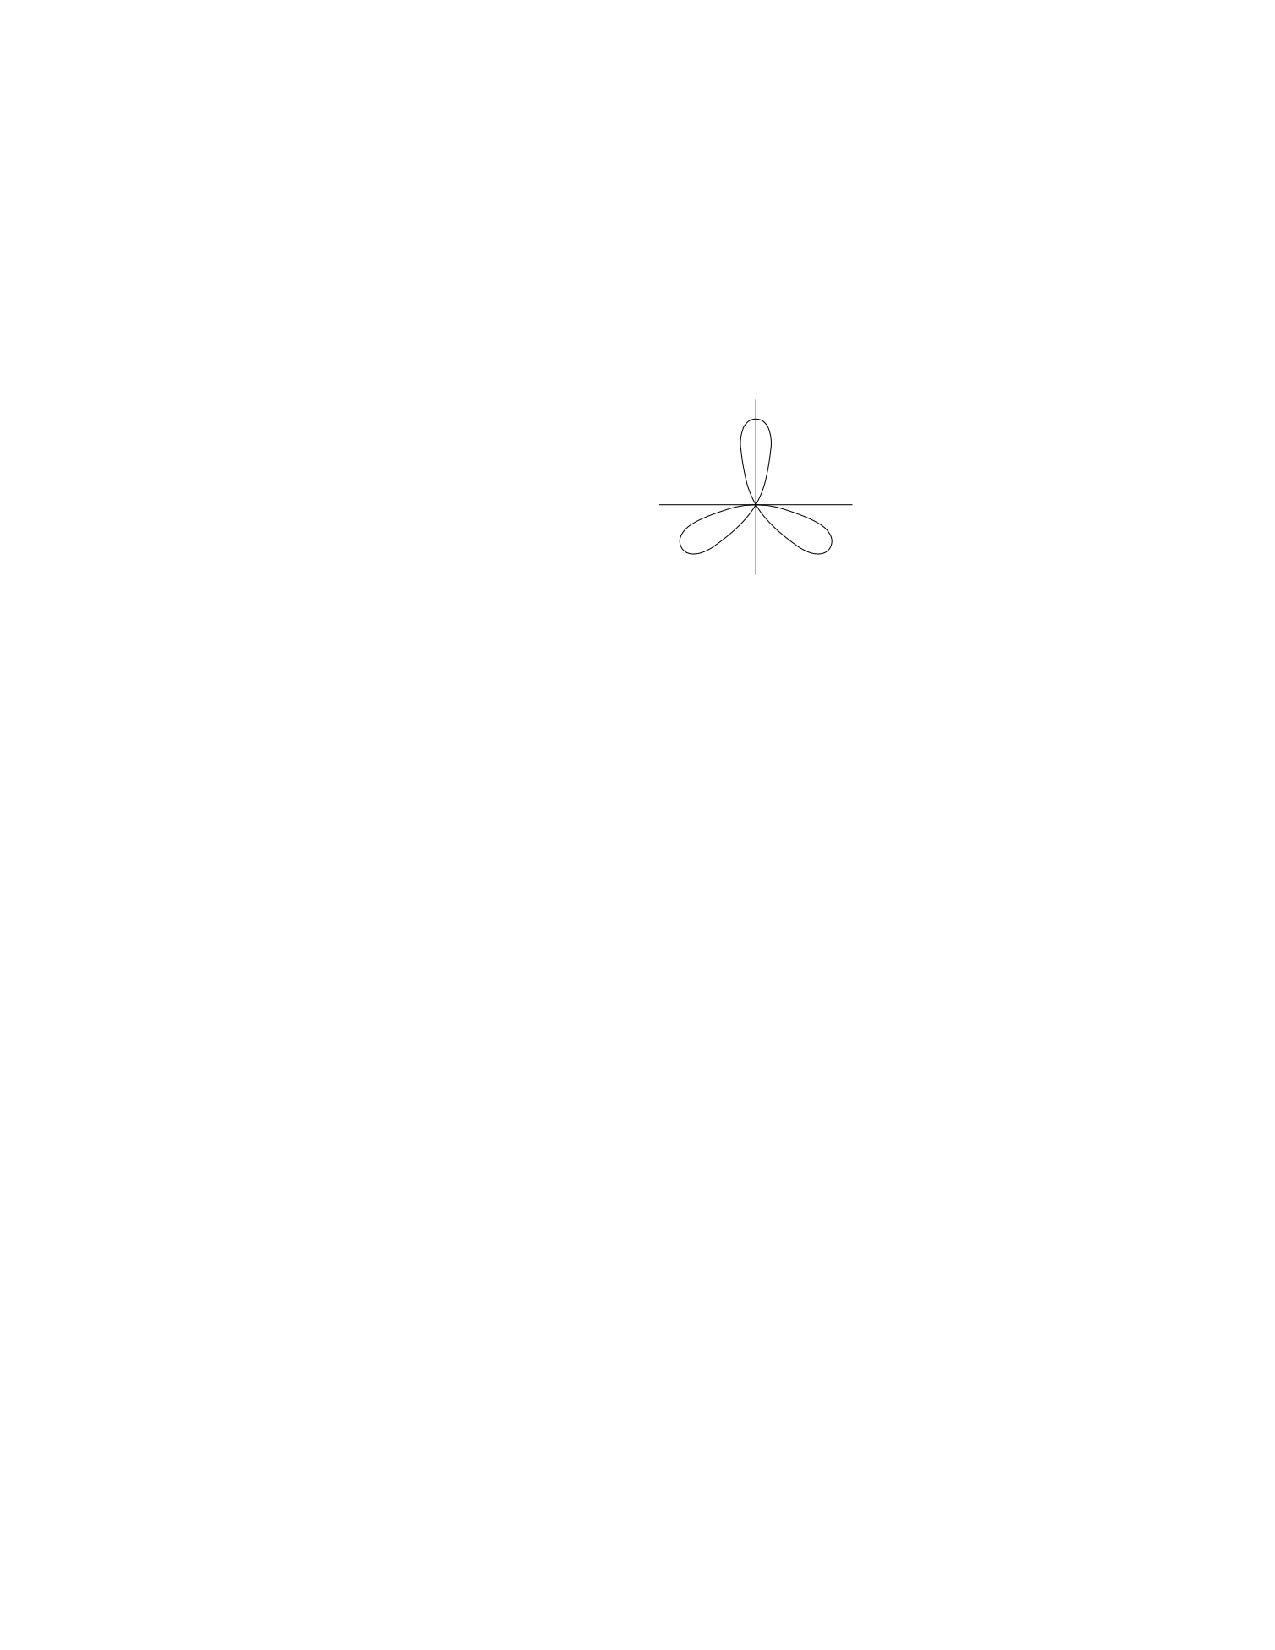
\includegraphics[height=0.4\linewidth]{4c}\quad\quad
		
\includegraphics[height=0.4\linewidth]{4d}
		\caption{\small$F=x^3+x^2-y^2$ \quad$F=(x^2 + y^2)^3- 4x^2y^2$}
		\caption{\small\textit{\color{duongvaotoanhoc}Hình $4$. Các đường cong với kỳ dị tại $O(0,0)$.}}
		\vspace*{-5pt}
	\end{figure}
	Trong các đồ thị ở hình $4$, giá trị $m$ tương ứng là $2,2,3,4$. Phương trình
	$F_m=0$
	tương ứng là:
	\begin{align*}
		y^2&=0\\
		x^2-y^2&=0\\
		3x^2y-y^3&=0\\
		4x^2y^2&=0.
	\end{align*} 
	Các phương trình này xác định các chùm đường thẳng (bao gồm cả đường thẳng kép) là các tiếp tuyến tới đường cong tại $O$. 
	\vskip 0.1cm
	Ta thấy giá trị của $m$ ứng với số các tiếp tuyến tới đường cong tại điểm $O$. Lý giải cho điều này rất đơn giản. 
	\vskip 0.2cm
	\PIbox{Trong một {\em lân cận đủ nhỏ} của $O$, $F$ được xấp xỉ bởi $F_m$, do đó đường cong  $F$  được xấp xỉ bởi đường cong $F_m$.}
	\vskip 0.2cm
	Mở rộng phân tích ở trên cho một điểm bất kỳ trên đường cong ta có định nghĩa sau. 
	Cho $F\in \mathbb C[x,y]$ là đa thức bất khả quy và $P(a,b)$ là một điểm trên đường cong $F$. 
	\vskip 0.2cm
	\PIbox{Bội của $P$ trên đường cong, ký hiệu là $\mu_P(F)$, là lũy thừa nhỏ nhất trong khai triển Taylor của $F$ tại $P$:
		\setlength{\abovedisplayskip}{5pt}
		\setlength{\belowdisplayskip}{5pt}
	\begin{align*}
		F(x,y)= &F_m(x-a,y-b)\\
		&+F_{m+1}(x-a,y-b)+\ldots
	\end{align*}
		Phương trình
		$F_m(x-a,y-b)=0$
		xác định các đường thẳng tiếp xúc với đương cong tại $P$. }
	\vskip 0.2cm
	Nếu hai đường cong $F$  và $G$  cắt nhau tại điểm $P$, thì bội giao tại $P$ của hai đường cong phụ thuộc vào vị trí tương đối của các tiếp tuyến của hai đường cong. Trong trường hợp các tiếp tuyến là đôi một phân biệt thì bội giao sẽ là tích của số các tiếp tuyến. Nhưng trong trường hợp có sự trùng lấp thì vấn đề chưa rõ ràng. 
	\vskip 0.1cm
	Về nguyên tắc, để xác định được bội giao, người ta thực hiện một phép biến dạng nhỏ hai đường cong tại lân cận của giao điểm, sau đó đếm số giao điểm của hai đường cong trong lân cận đó. Đó là phương pháp của Giải tích. Trong Hình học Đại số, ta sẽ sử dụng tiếp cận khác, trong đó ta sẽ trừu tượng hóa vấn đề lên để qua đó nhìn thấy sâu hơn bản chất của nó. Bội giao của hai đường cong sẽ được nhìn nhận như chiều của các không gian véc tơ. Công cụ để triển khai việc này là {\em vành địa phương}. 
	\vskip 0.1cm
	$\pmb{5.}$ \textbf{\color{duongvaotoanhoc}Vành địa phương và bội của điểm trên đường cong} 
	\vskip 0.1cm 
	Thay vì xác định bội của một điểm trên đường cong như là số các giao điểm nào đó, ta có thể xác định số bội này thông qua vành địa phương. Ý tưởng mấu chốt ở đây là vành địa phương tại một điểm trên đường cong {\em chứa toàn bộ thông tin về hình học} của đường cong trong lân cận của điểm đó. Sau khi đã nhìn thấy điều đó thì việc xây dựng các công thức là vấn đề mang tính kỹ thuật. 
	\vskip 0.1cm
	Nhắc lại rằng số bội của một điểm $P$ trên đường cong $F$ được xác định nhờ khai triển Taylor của $F$ tại điểm đó. Ta sẽ định nghĩa số bội này thông qua số chiều của các không gian véc tơ được xây dựng từ vành địa phương của $P$.  Ưu điểm của cách làm này là nó cho một mô tả trừu tượng về số bội, cho chúng ta hiểu biết sâu sắc hơn về nó, để từ đó cho phép phát triển những phương pháp hiện đại hơn khi nghiên cứu số bội. 
	\vskip 0.1cm
	{\em Vành địa phương tại một điểm trong mặt phẳng affine} (phức) được hiểu là tập các hàm số xác định trên một lân cận nào đó của điểm đã cho. Do ta chỉ xét các hàm ``đại số'' nên định nghĩa của một hàm địa phương là như sau.
	\vskip 0.2cm
	\PIbox{Vành địa phương $\pazocal O_P$ tại điểm $P(a,b)$ trong mặt phẳng affine là tập hợp các phân thức đại số $F/G$ với tính chất
		$G(P):=G(a,b)\neq 0.$}
	\vskip 0.2cm
	Tập hợp các phân thức trong $\pazocal O_P$ triệt tiêu tại $P$ lập thành ideal cực đại duy nhất trong vành này, ký hiệu là $\mathfrak m_P$. 
	\begin{align*}
		\mathfrak m_P=\left\{ F/G \left|\right.  F(P)=0, G(P)\neq 0\right\}.
	\end{align*}
	Trong Đại số Giao hoán, một vành với duy nhất ideal cực đại được gọi   là \textbf{\color{duongvaotoanhoc}vành địa phương}.
	\vskip 0.1cm
	Cho $P(a,b)$ là một điểm trên đường cong bất khả quy  $F$. Các hàm địa phương trên mặt phẳng affine tại $P$ khi hạn chế lên đường cong này xác định các hàm địa phương trên đó. Ta nhận thấy rằng hai hàm khi hạn chế lên đường cong sẽ bằng nhau nếu chúng sai khác nhau bởi một bội số của $F$. Do đó, 
	\vskip 0.2cm
	\PIbox{vành các hàm địa phương tại $P$ trên đường cong $F$  là vành thương 
		$\pazocal O_P(F):= \pazocal O_P/(F),$}
	\vskip 0.2cm
	trong đó $(F)$ là ideal sinh bởi $F$ trong vành $\pazocal O_P$.
	Vành $\pazocal O_P(F)$ cũng là vành địa phương với ideal cực đại duy nhất:
	$\mathfrak m_P(F)=\mathfrak m_P/(F).$
	\vskip 0.1cm
	\textbf{\color{duongvaotoanhoc}Mệnh đề} $\pmb{4}$ (Bội của điểm trên đường cong)\textbf{\color{duongvaotoanhoc}.} 
		\textit{Cho $F\in\mathbb C[x,y]$ là đa thức bất khả quy và $P$ là một điểm trên đường cong $F$. 
		Khi đó với mọi $n\geq\mu:= \mu_P(F)$  ta có}
		\setlength{\abovedisplayskip}{8pt}
		\setlength{\belowdisplayskip}{8pt} 
		\begin{align*}
			\dim_{\mathbb C}  \pazocal O_P(F)/(\mathfrak m_P(F)^n)=\mu \cdot n -
			{\mu \choose 2}.
		\end{align*}
	\vskip 0.1cm
	Trong trường hợp $P$ là một điểm đơn trên đường cong, nghĩa là $\mu_P(F)=1$, từ công thức trên ta suy ra:
	\begin{align*}
		\dim_{\mathbb C} \mathfrak m_P(F)^n/\mathfrak m_P(F)^{n+1}=1
	\end{align*}
	với mọi $n$. 
	\vskip 0.1cm
	$\pmb{6.}$ \textbf{\color{duongvaotoanhoc}Giao điểm của hai đường cong}
	\vskip 0.1cm
	Xét hai đường cong $F$  và $G$. Khi đó hệ phương trình
	\begin{align*}
		\begin{cases}
			F = 0\\
			G = 0
		\end{cases}
	\end{align*}
	xác định tập giao của hai đường cong này.  
	\vskip 0.1cm
	\textbf{\color{duongvaotoanhoc}Định lý} $\pmb{5.}$ \textit{Giả thiết hai đường cong $F$  và $G$  không chứa chung một thành phần, khi đó chúng giao nhau tại một tập hữu hạn điểm.}
	\vskip 0.1cm
	\textit{Chứng minh.}
	Theo giả thiết thì hai đa thức $F$ và $G$ không có ước chung trong $\mathbb C[x,y]$. Khi đó hai đa thức này cũng không có ước chung trong $\mathbb C(x)[y]$ -- tập các đa thức theo $y$ với hệ số trong $\mathbb C(x)$. Từ đó, theo bổ để B\'ezout, tồn tại hai đa thức $A$ và $B$ trong  $\mathbb C(x)[y]$ sao cho
	\begin{align*}
		1=AF+BG.
	\end{align*}
	Sau khi quy đồng mẫu số các hệ số của $A$ và $B$ ta thu được đẳng thức
	\begin{align*}
		C= A'F+ B'G,
	\end{align*}
	với $0\neq C\in\mathbb C[x]$, $ A', B'\in \mathbb C[x,y]$. 
	Như vậy nghiệm của hệ $(F=0, G=0)$ có tọa độ theo trục $x$ là nghiệm của đa thức {\em một biến} $C$, do đó là tập hữu hạn. Lý luận tương tự đối với tọa độ $y$ ta suy ra điều phải chứng minh. 
	\vskip 0.1cm
	$\pmb{7.}$ \textbf{\color{duongvaotoanhoc}Xạ ảnh hóa mặt phẳng affine} 
	\vskip 0.1cm
	Trong mặt phẳng affine phức, tồn tại các đường cong không giao nhau tại điểm nào, ví dụ hai đường thẳng song song. 
	Đây có thể được hiểu như một trường hợp {\em suy biến}. Xét hệ sau:
	\begin{align*}
		\begin{cases}
			\alpha x+y+1 =0\\
			y=0
		\end{cases}
	\end{align*}
	Với mọi $\alpha\neq 0$, hệ có duy nhất nghiệm, với $\alpha=0$, hệ vô nghiệm. 
	\vskip 0.1cm
	Ta hình dung khi $\alpha$ {\em tiến tới} $0$, giao điểm của hai đường thẳng $y=0$ và $\alpha x+y+1=0$ {\em chạy ra vô cùng}. Ta sẽ bổ sung {\em điểm ở vô cùng} này vào mặt phẳng affine. Mỗi đường thẳng trên mặt phẳng affine sẽ xác định một điểm ở vô cùng. Hai đường thẳng song song cùng xác định một điểm tại vô cùng là điểm mà chúng cắt nhau. 
	\vskip 0.1cm
	Mặt phẳng affine bổ sung thêm các điểm ở vô cùng được gọi là {\em mặt phẳng xạ ảnh}. Các điểm trong mặt phẳng xạ ảnh (thực hoặc phức) được mô tả thuận tiện nhất thông qua các tọa độ thuần nhất. Một tọa độ thuần nhất là một dãy tỷ lệ $[a_0:a_1:a_2]$ trong đó có ít nhất một trong các tọa độ $a_i\neq 0$. Nhắc lại rằng hai dãy tỷ lệ $[a_0:a_1:a_2]$ và $[b_0:b_1:b_2]$ được gọi là bằng nhau nếu tồn tại $\lambda\neq 0$ sao cho
	\begin{align*}
		a_i=\lambda b_i, \quad i=0,1,2.
	\end{align*}
	Một điểm trong mặt phẳng affine với tọa độ $(a_0,a_1)$ sẽ có tọa độ thuần nhất $[a_0:a_1:1]$. Các điểm ở vô cùng có tọa độ dạng $[a_0:a_1:0]$ (với ít nhất một trong hai số $a_0$, $a_1$ khác $0$). Điểm này ứng với đường thẳng chứa các điểm $(\lambda a_0,\lambda a_1)$ trên mặt phẳng affine. 
	\vskip 0.1cm	
	Các đường thẳng trong không gian xạ ảnh thông thường được tạo thành từ một đường thẳng trong không gian affine và một điểm ở vô cùng. Ngoại lệ duy nhất là đường thẳng ở vô cùng -- nó bao gồm tất cả các điểm ở vô cùng.
	Phương trình đường thẳng trong mặt phẳng xạ ảnh có dạng
	\begin{align*}
		aX+bY+cZ=0,
	\end{align*}
	trong đó có ít nhất một trong các hệ số $a,b,c$ khác $0$. Phương trình
	$Z=0$ 
	xác định {\em đường thẳng ở vô cùng} -- rõ ràng các nghiệm của nó có dạng $[a:b:0]$.
	\vskip 0.1cm
	Với mỗi đa thức $F\in \mathbb C[x,y]$, ta định nghĩa đa thức $\widehat F(X,Y,Z)\in \mathbb C[X,Y,Z]$ theo công thức
	\begin{align*}
		\widehat F(X,Y,Z):=Z^{\deg F}F(X/Z,Y/Z).
	\end{align*}
	Trong đa thức $\widehat F$ tất cả các đơn thức đều có cùng bậc, chính là bậc của đa thức $ F$ ban đầu. Ta nói $\widehat F$ là một {\em đa thức thuần nhất}. 
	Các điểm trong mặt phẳng xạ ảnh với tọa độ thuần nhất là nghiệm của phương trình
	\begin{align*}
		\widehat F(X,Y,Z)=0
	\end{align*}
	xác định một đường cong trong không gian xạ ảnh, được gọi là  {\em xạ ảnh hóa} của đường cong $F$. 
	\vskip 0.1cm
	Các điểm ở vô cùng của đường cong xạ ảnh hóa ứng với nghiệm chung của hai  phương trình 
	$\widehat F=0,\ Z=0.$
	Hay nói cách khác, là nghiệm của phương trình
	\begin{align*}
		\widehat F(X,Y,0)=0.
	\end{align*}
	Xét khai triển Taylor của $F$ tại $(0,0)$:
	\begin{align*}
		F=F_0+F_1+\ldots + F_m.
	\end{align*}
	Khi đó $F_i$ là tổng tất cả các đơn thức bậc $i$ trong $F$. Do đó 
	\begin{align*}
		\widehat F(X,Y,0)= F_m(X,Y).
	\end{align*}
	Vậy các điểm ở vô cùng của $F$  là các điểm có tọa độ thuần nhất $[a:b:0]$ trong đó $(a,b)$ là nghiệm không tầm thường của $F_m=0$.
	\vskip 0.1cm
	\textbf{\color{duongvaotoanhoc}Ví dụ.} Xét đường cong $xy-1=0$. Xạ ảnh hóa ta thu được đường cong
	\begin{align*}
		XY-Z^2=0.
	\end{align*}
	Giao của nó với đường thẳng ở vô cùng $Z=0$ được xác định bởi phương trình
	$XY=0.$
	Vậy ta có hai điểm $[1:0:0]$ và $[0:1:0]$ ứng với hai tập nghiệm $(a,0)$ và $(0,b)$ của phương trình trên. Hai điểm ở vô cùng này tương ứng với điểm $(0,0,0)$ trên mặt paraboloid tròn xoay mô tả ở mục $1$ (điểm còn lại là điểm ở vô cùng của mặt paraboloid).   
	\vskip 0.1cm
	Trong mặt phẳng xạ ảnh phức, hai đường thẳng bất kỳ luôn cắt nhau. Điều này cũng đúng với các đường cong bất kỳ. 
	\vskip 0.1cm
	\textbf{\color{duongvaotoanhoc}Mệnh đề} $\pmb{6.}$
	\textit{Hai đường cong đại số trong mặt phẳng xạ ảnh luôn giao nhau.}
	\vskip 0.1cm
	$\pmb{8.}$ \textbf{\color{duongvaotoanhoc}Bội giao của hai đường cong tại một điểm} 
	\vskip 0.1cm 
	Chúng ta sẽ minh họa định nghĩa bội giao của hai đường cong bất khả quy $F$  và $G$  tại một điểm $P$ trong trường hợp $P$ là điểm đơn trên $F$.  Giả thiết $P$ là gốc tọa độ. Trong một lân cận đủ nhỏ của $P$, $F$  có thể được xấp xỉ bởi một đường thẳng, giả sử là $x=0$. Khi đó số giao điểm của hai đường cong tại $P$ bằng số nghiệm (kể cả bội) của phương trình 
	\begin{align*}
		G(0,y)=0
	\end{align*}
	trong một lân cận của $0$. Như vậy ta có thể thay $G$ bằng cách nhân với một hàm không triệt tiêu trong một lân cận của $P$ mà không làm thay đổi số nghiệm. Chẳng hạn, ta có thể biến đổi $G$ để 
	\begin{align*}
		G(0,y)=\prod_{j=1}^d(y-b_j),
	\end{align*}
	với các số $b_j$ nằm trong một lân cận đủ nhỏ của $0$, với $d$ là số giao điểm. Theo tinh thần ở mục trước $d$ chính là chiều của không gian véc tơ
	\begin{align*}
		\pazocal O_P/(F,G).
	\end{align*}
	Đây là cơ sở cho định nghĩa sau.
	\vskip 0.2cm
	\PIbox{Bội giao của hai đường cong $F$  và $G$  tại điểm $P$ được định nghĩa là số
	\begin{align*}
		\mu_P(F,G):=\dim_{\mathbb C}\pazocal O_P/(F,G).
	\end{align*}}
	\vskip 0.05cm
	Đối với mọi điểm $B$ không là giao điểm ta định nghĩa
	$\mu_B(F,G)=0.$ 
	Ta có các tính  chất cơ bản sau đây của bội giao. 
	\vskip 0.1cm
	($1$) Nếu các đa thức $G$ và $H$ không có ước chung với $F$ thì
	\setlength{\abovedisplayskip}{7pt}
	\setlength{\belowdisplayskip}{7pt} 
	\begin{align*}
		\mu_P(F,GH)=\mu_P(F,G)+\mu_P(F,H).
	\end{align*}
	($2$) $\mu_P(F,G)\geq \mu_P(F)\cdot \mu_P(G)$ với dấu bằng xảy ra khi và chỉ khi $F$ và $G$ không có chung tiếp tuyến tại $P$;
	\vskip 0.1cm
	($3$) Nếu $P$ là điểm đơn trên $F$  thì $\mu_P(F,G)$ bằng định giá của $G$ trong vành $\pazocal O_P(F)$. 
	\vskip 0.1cm
	\textbf{\color{duongvaotoanhoc}Định lý} $\pmb{7}$ (Bézout)\textbf{\color{duongvaotoanhoc}.} \textit{Cho $\widehat F=0$ và $\widehat G=0$ là hai đường cong  trong mặt phẳng xạ ảnh với bậc tương ứng là $m$ và $n$. Giả sử chúng không có thành phần chung. Khi đó}
	\begin{align*}
		\sum_P\mu_P(\widehat F,\widehat G)=m\cdot n.
	\end{align*}
	Giả sử giao điểm của  $\widehat F=0$ và $\widehat G=0$ đều nằm trong mặt phẳng affine $Z\neq 0$. 
	Khi đó  định lý Bézout là hệ quả của hai mệnh đề:
	\vskip 0.1cm
	($1$) Đặt $F(x,y):=\widehat F(x,y,1)$, $G(x,y):=\widehat G(x,y,1)$, thì 
		\begin{align*}
			\sum_P\mu_P(\widehat F,\widehat G)=\dim_{\mathbb C}R/(F,G);
		\end{align*}
	($2$) Nếu hai đường cong $F$  và $G$  không giao nhau tại vô cùng thì 
		\begin{align*}
			\dim_{\mathbb C}\mathbb C[x,y]/(F,G)= m\cdot n.
		\end{align*}
	Mệnh đề ($1$) là hệ quả của đẳng cấu
	\begin{align*}
		\varphi:\mathbb C[x,y]/(F,G)\simeq \prod_P \pazocal O_P/(F,G).
	\end{align*}
	Nói cách khác, {\bf\color{duongvaotoanhoc} vành tọa độ} của giao hai đường cong là tích của các vành địa phương tại mỗi giao điểm.
	\vskip 0.1cm
	Mệnh đề ($2$) được rút ra từ  \textbf{\color{duongvaotoanhoc}dãy khớp}  sau đây. Đặt $R:=\mathbb C[x,y]$ và $R_d$ là tập các đa thức trong $R$ với bậc $<d$.
	Với mỗi $d\geq m+n$, dãy các ánh xạ tuyến tính sau là khớp (nghĩa là ảnh của ánh xạ trước trùng với hạch của ánh xạ sau):
	\begin{align*}
		0&\longrightarrow R_{d-m-n}\stackrel\beta\longrightarrow 
		R_{d-m}\oplus R_{d-n} \stackrel\alpha\longrightarrow R_d\\
		&\stackrel\pi\longrightarrow R/(F,G)\longrightarrow 0	
	\end{align*}
	trong đó  
	\begin{align*}
		&\alpha: (A,B)\longmapsto AF+BG,\\
		&\beta: C\longmapsto (CG,-CF),
	\end{align*}
	còn $\pi$ là hạn chế của ánh xạ thương lên $R_d$. Từ đó, bằng cách so sánh số chiều ta có 
	\begin{align*} \dim_{\mathbb C}\textrm{im}\pi=&\dim_{\mathbb C}R_d-\dim_{\mathbb C}\textrm{ker}\pi\\
		=& \dim_{\mathbb C}R_d-\dim_{\mathbb C}\textrm{im}\alpha\\
		=& \dim_{\mathbb C}R_d-\dim_{\mathbb C}R_{d-m}\\
		&-\dim_{\mathbb C}R_{d-n}+ 
		\dim_{\mathbb C}R_{d-m-n}.
	\end{align*}
	Do
	\begin{align*}
		\dim_{\mathbb C}R_k={k+1\choose 2}
	\end{align*}
	ta thu được 
	\begin{align*}
		\dim_{\mathbb C}\textrm{im}\pi=  m\cdot n.
	\end{align*}
	Nhận xét rằng trong các chứng minh đều xuất hiện biểu thức dạng
	\begin{align*}
		AF+BG.
	\end{align*}
	Biểu thức này rõ ràng có nguồn gốc từ khai triển Bézout cũng như liên quan tới kết thức của hai đa thức. 
	\vskip 0.1cm
	\textbf{\color{duongvaotoanhoc}Lời cảm ơn:} Tác giả trân trọng cảm ơn TS.~Nguyễn Đăng Hợp và TS. Đào Văn Thịnh đã đọc kỹ và có nhiều góp ý giá trị giúp hoàn thiện bài viết.  
	\vskip 0.1cm
	\textbf{\color{duongvaotoanhoc}Tài liệu tham khảo}
	\vskip 0.1cm
	[$1$]  W. Fulton. {\em Algebraic curves, An Introduction into Algebraic Geometry}, $2008$.\\
	\url{https://dept.math.lsa.umich.edu/~wfulton/CurveBook.pdf}
	\vskip 0.1cm
	[$2$]  A. Gathmann. {\em Plane Algebraic Curves}, TU Kaiserslautern $2018$.\\ 
	\url{https://www.mathematik.uni-kl.de/~gathm}\\ \url{ann/class/curves-2018/curves-2018.pdf}
	\vskip 0.1cm	
	[$3$] Ngô Việt Trung. {\em Nhập môn Đại số Giao hoán $\&$ Hình học Đại số}, NXB Khoa học Tự nhiên và Công nghệ, $2012$.
\end{multicols} 
	\newpage

	\setcounter{figure}{0}
	\thispagestyle{quantoannone}
\pagestyle{quantoan}
\everymath{\color{quantoan}}
\graphicspath{{../quantoan/pic/}}
\blfootnote{\color{quantoan}\color{quantoan}$^1$Viện Toán học.}
\begingroup
\AddToShipoutPicture*{\put(0,616){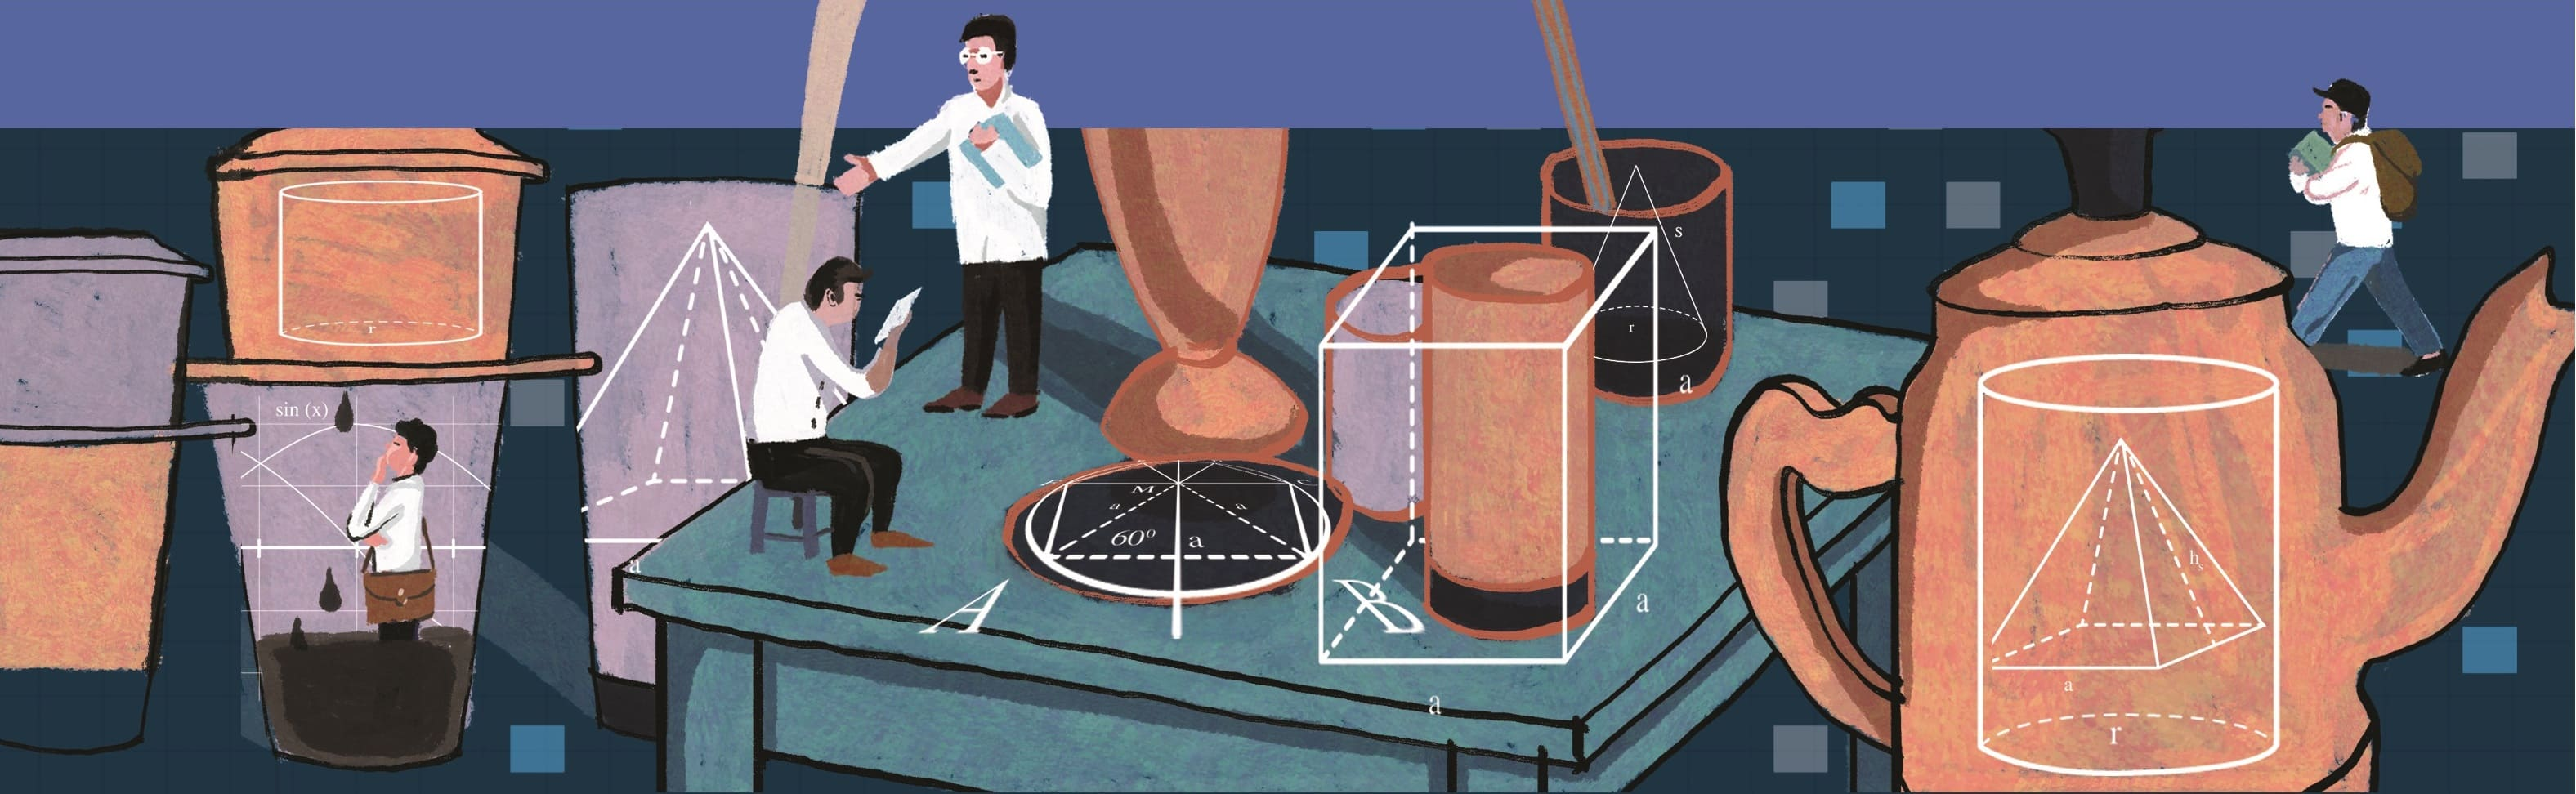
\includegraphics[width=19.3cm]{../bannerquantoan}}}
\AddToShipoutPicture*{\put(156,550){
\includegraphics[scale=1]{../tieude3.pdf}}}
\centering
\endgroup

\vspace*{160pt}

\begin{multicols}{2}	
	Ngày nay số âm đã được học sinh làm quen từ lớp $6$. Nhưng nhân loại đã mất tới $2000$ năm để có thể chấp nhận được nó như cách mà học sinh lớp $6$ ngày nay chấp nhận. 
	\begin{figure}[H]
		\vspace*{-5pt}
		\centering
		\captionsetup{labelformat= empty, justification=centering}
		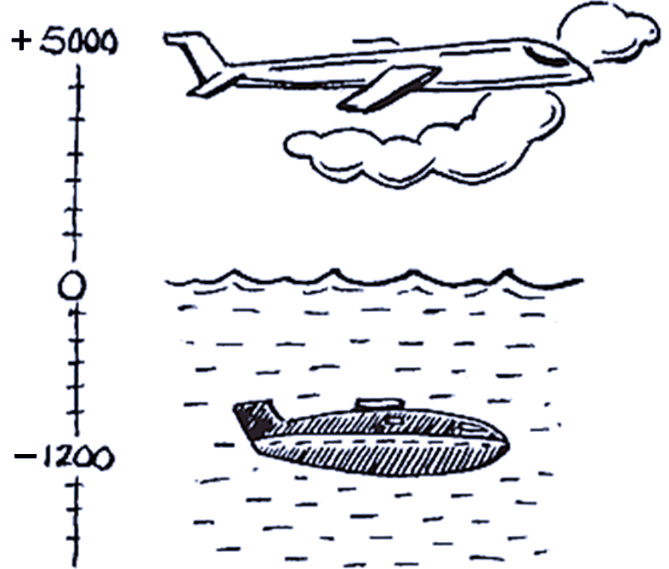
\includegraphics[width= 1\linewidth]{1}
%		\caption{\small\textit{\color{}}}
		\vspace*{-10pt}
	\end{figure}
	Nhìn lại lịch sử cho chúng ta thấy sự vật lộn trong quá trình trừu tượng hóa của Toán học. Hy vọng, theo dõi quá trình vất vả này, các thầy cô giáo THCS sẽ có thêm sự cảm thông đối với những học sinh ``dốt toán". Biết đâu, các em có thể không dốt mà chỉ đang vật lộn với việc phản biện như những nhà toán học kiệt xuất đã từng phản biện về số âm? 
	\vskip 0.1cm
	-- Thế kỷ V TCN, Hy Lạp: Trường phái Pythagoras coi số là ``nhiều đơn vị". Vì vậy với họ ``một" không phải là một số. Không có dấu hiệu nào về số âm trong các ghi chép của họ.
	\vskip 0.1cm
	-- Thế kỷ IV TCN, Hy Lạp: Aristotle đã đưa ra sự phân biệt giữa số (tức là số tự nhiên) và độ lớn (``số đó chia hết thành các số chia mà có thể chia vô hạn"), nhưng không đưa ra dấu hiệu nào về khái niệm số âm hoặc độ lớn âm.
	\vskip 0.1cm
	-- Khoảng năm $300$ TCN, Hy Lạp: Các tập VII, VIII và IX trong cuốn \textit{Cơ sở} của Euclid liên quan đến lý thuyết cơ bản về số. Euclid tiếp tục sự phân biệt của Aristotle giữa số và độ lớn, nhưng vẫn không có dấu hiệu nào về số âm.
	\vskip 0.1cm
	-- Thế kỷ I TCN -- thế kỷ I, Trung Quốc: Trong \textit{Cửu chương Toán thuật}, số âm đã được sử dụng trong chương về giải hệ phương trình. Các que màu đỏ được sử dụng để biểu thị các hệ số dương, màu đen để biểu thị các hệ số âm. Các quy tắc cho số có dấu đã được đưa ra.
	\vskip 0.1cm
	-- Thế kỷ III, Hy Lạp: Dấu hiệu đầu tiên về số âm trong một tác phẩm phương Tây xuất hiện trong cuốn \textit{Số học} của Diophantus, trong đó ông gọi phương trình mà trong ký hiệu hiện đại sẽ được biểu thị bởi $4x + 20 = 0$ là ``vô lý", vì nó sẽ cho nghiệm $x=-5$. Ông cũng nói, ``một số bị trừ, nhân với một số bị trừ, cho một số được cộng (thêm vào)". Vì vậy ông có thể xử lý các biểu thức chẳng hạn như $(x-1)(x-2)$, trong ký hiệu hiện đại. Tuy nhiên, có thể tìm thấy những chỉ dẫn trong tác phẩm của Diophantus rằng ông không có khái niệm trừu tượng về số âm.
	\vskip 0.1cm
	-- Thế kỷ VII, Ấn Độ: Số âm được sử dụng để biểu thị các khoản nợ trong khi số dương biểu thị tài sản. Nhà toán học và thiên văn học Brahmagupta đã sử dụng các số âm để thống nhất phương pháp xử lý phương trình bậc hai của Diophantus từ ba trường hợp thành một trường hợp duy nhất mà chúng ta quen thuộc ngày nay.
	\vskip 0.1cm
	-- Thế kỷ IX, Trung Đông: Mặc dù người Ả Rập đã quen thuộc với các số âm từ công trình của các nhà toán học Ấn Độ, nhưng họ bác bỏ chúng. Cuốn sách \textit{al--Kitāb al--Mukhtaṣar fī Ḥisāb al--Jabr wal--Muqābalah} (mà từ đó chúng ta có thuật ngữ ``algebra" -- đại số) của Muhammad ibn Musa al--Khwarizmi không sử dụng số âm hoặc hệ số âm.
	\vskip 0.1cm
	-- Thế kỷ XIII, Trung Quốc: Các số âm được biểu thị bằng cách vẽ một nét chéo qua chữ số khác không ngoài cùng bên phải của số đó.
	\vskip 0.1cm
	-- Thế kỷ XIII, Châu Âu: Fibonacci không đề cập đến số âm trong cuốn sách \textit{Liber Abaci} của mình, nhưng trong cuốn \textit{Flos} sau đó, ông giải thích nghiệm âm như là sự thua lỗ.
	\vskip 0.1cm
	-- Thế kỷ XV, Châu Âu: Chuquet là người đầu tiên sử dụng số âm trong một tác phẩm ở Châu Âu.
	\vskip 0.1cm
	-- Thế kỷ XVI, Châu Âu: 
	\vskip 0.1cm
	$\circ$ Cardan (Cardano), trong cuốn sách \textit{Ars Magna} của mình đã đưa vào các nghiệm âm của các phương trình và nêu các quy luật cơ bản của hoạt động với các số âm. Ông gọi các số dương là thực và các số âm là hư cấu.
	\vskip 0.1cm
	$\circ$ Viete không thừa nhận số âm.
	\vskip 0.1cm
	-- Thế kỷ XVII, Châu Âu:
	\vskip 0.1cm
	$\circ$ Descartes chấp nhận một phần khái niệm số âm. Ông không công nhận nghiệm âm vì chúng đại diện cho các số ``nhỏ hơn không có gì". Tuy nhiên, ông đã chỉ ra rằng một phương trình có nghiệm âm có thể được biến đổi thành một phương trình có nghiệm dương, điều này khiến ông chấp nhận các số âm.
	\vskip 0.1cm
	$\circ$ Pascal coi phép ``trừ đi $4$ từ $0$" là điều hoàn toàn vô nghĩa.
	\vskip 0.1cm
	$\circ$ Nhà thần học và toán học Antoine Arnauld lập luận chống lại số âm bằng cách sử dụng tỷ lệ; nói rằng tỷ lệ $-1$ trên $1$ giống với tỷ lệ $1$ trên $-1$ là vô lý, vì ``Làm thế nào tỷ lệ giữa một anh nhỏ với một anh lớn hơn lại như giữa anh lớn hơn với anh nhỏ hơn?"
	\vskip 0.1cm
	-- Thế kỷ XVIII, Châu Âu:
	\vskip 0.1cm
	$\circ$ Leibniz đồng ý với lập luận của Arnaud đối với các số âm, nhưng nói rằng vì về hình thức các tỷ lệ như vậy là đúng, nên người ta vẫn có thể tính toán với chúng.
	\vskip 0.1cm
	$\circ$ Maclaurin đã xử lý các đại lượng âm ngang hàng với các đại lượng dương trong tác phẩm \textit{A Treatise of Algebra} của ông.
	\vskip 0.1cm 
	$\circ$ Euler mở đầu tác phẩm \textit{Nhập môn tổng quan về Đại số} với một thảo luận về các phép toán trên các đại lượng dương và âm. Ông sử dụng ví dụ về một khoản nợ để biện minh rằng một số âm lần số dương là một số âm.  
	\vskip 0.1cm
	-- Thế kỷ XIX, Châu Âu: Hamilton đã cố gắng đưa các số âm lên một nền tảng lý thuyết vững chắc (thay vì khái niệm về đại lượng ``nhỏ hơn không có gì") bằng cách sử dụng ý tưởng về ``thời gian thuần túy" xuất phát từ tác phẩm \textit{Phê bình lý tính thuần túy} của Kant. Nỗ lực này có vẻ khá kỳ lạ đối với chúng ta ngày nay, nhưng nó đã giúp ích trong việc phát triển các \textit{quaternion}, ví dụ đầu tiên về một hệ đại số không thỏa mãn tính giao hoán.
	\begin{flushright}
		Theo \url{https://web.ma.utexas.edu/users/mks/326K/Negnos.html}
	\end{flushright}
\end{multicols}
	\newpage

%	\thispagestyle{empty}
%	\begingroup 
%	\AddToShipoutPicture*{\put(0,0){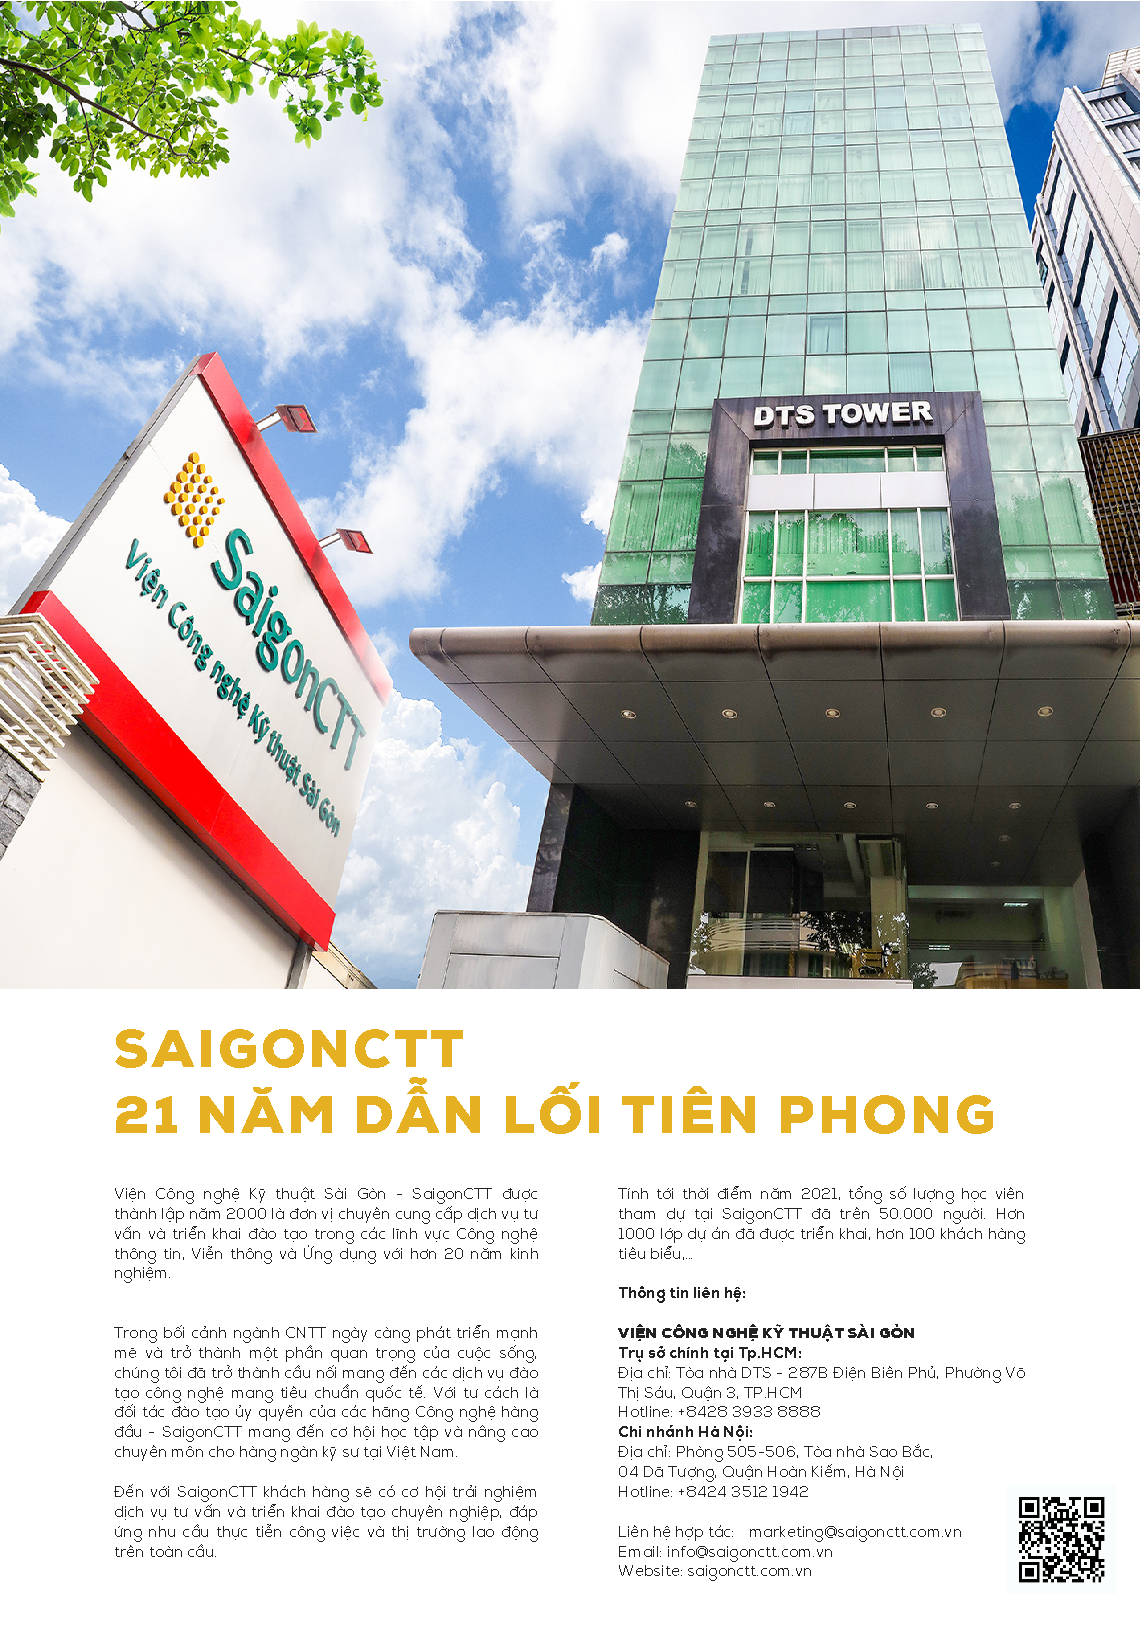
\includegraphics[scale=1]{DTS.pdf}}}
%	\centering
%	\vspace*{0cm}
%	\endgroup
%	\newpage	
%	\pagestyle{empty}
	
	\setcounter{figure}{0}
	\thispagestyle{toancuabinone}
\pagestyle{toancuabi}
\everymath{\color{toancuabi}}
%\blfootnote{$^1$\color{toancuabi}Đại học Thăng Long.}
\graphicspath{{../toancuabi/pic/}}
\begingroup
\AddToShipoutPicture*{\put(0,616){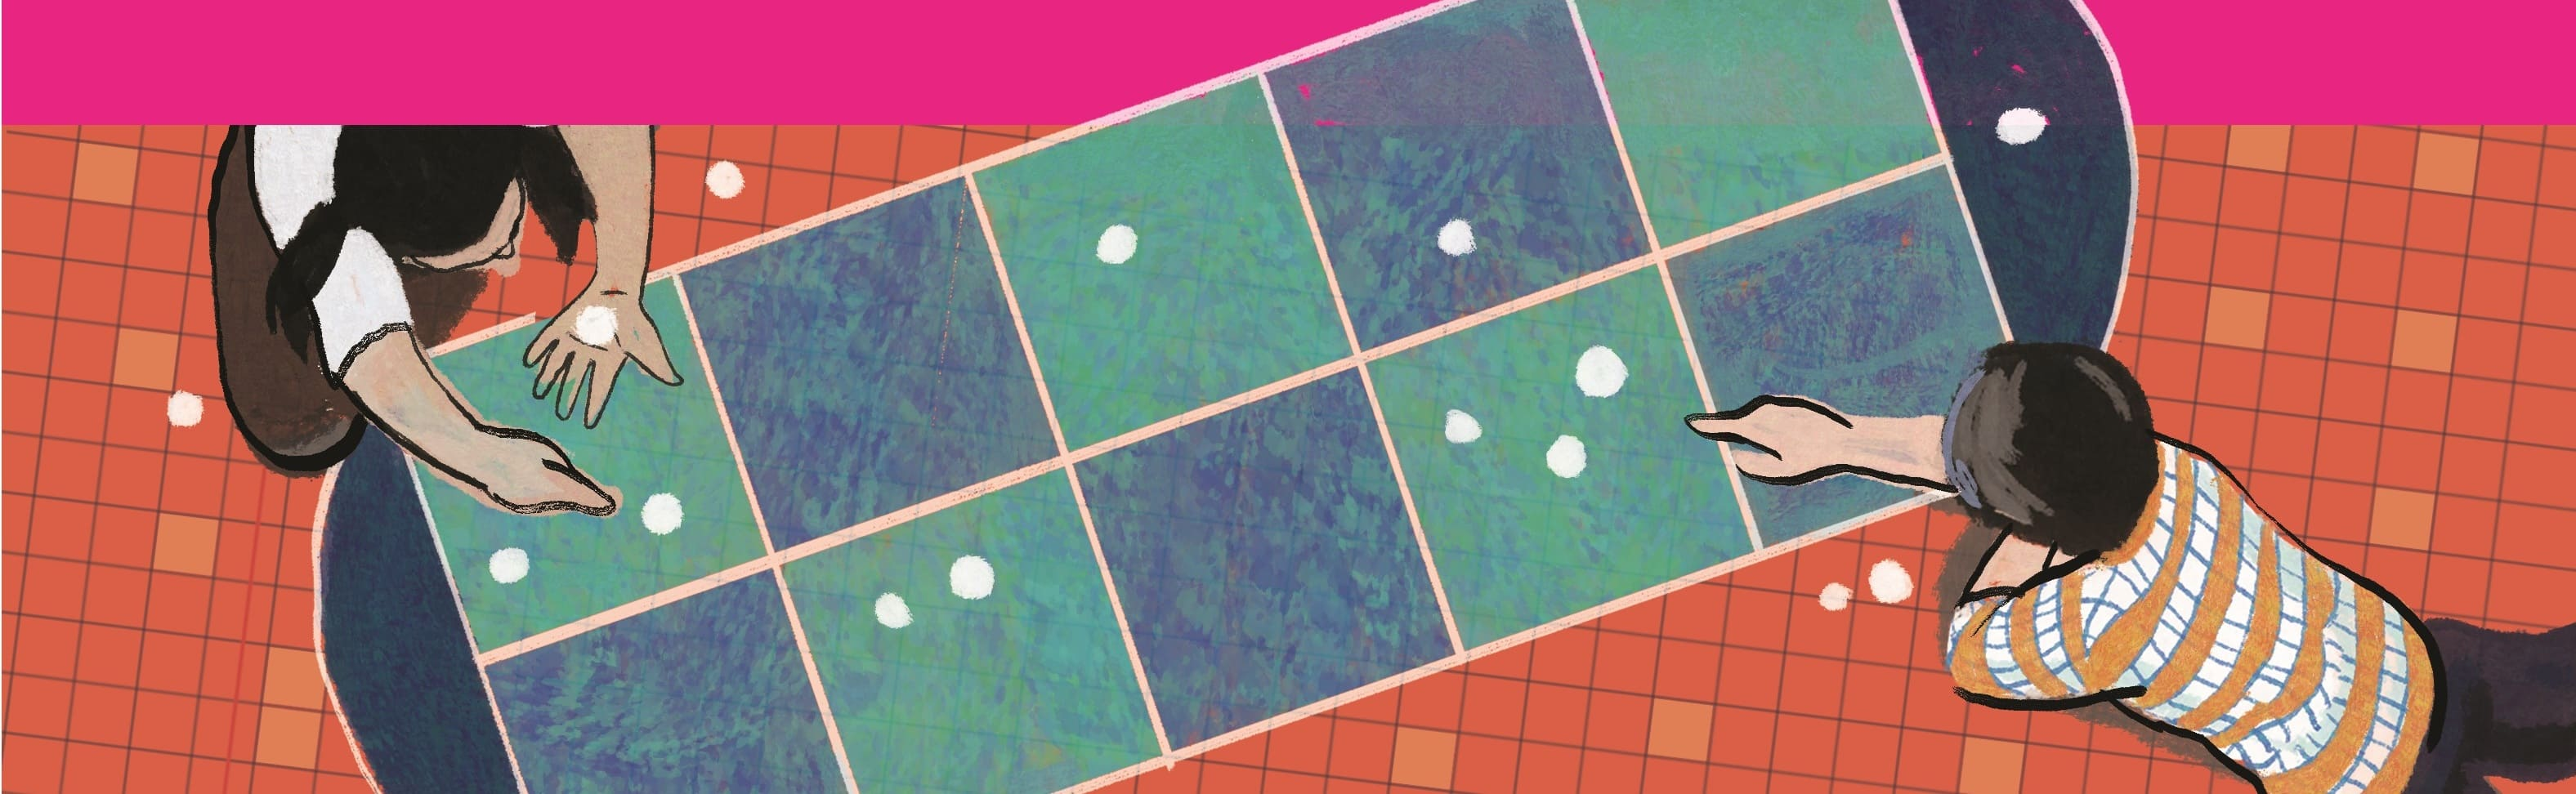
\includegraphics[width=19.3cm]{../bannertoancuabi}}}  
\AddToShipoutPicture*{\put(85,525){
\includegraphics[scale=1]{../tieude1.pdf}}} 
\centering
\endgroup

\vspace*{180pt}

\begin{multicols}{2}
	Mục Toán của Bi trong Số $11$, Tập $6$ đã giới thiệu đến các em cách tính diện tích của những hình tạo trên lưới ô vuông. Rất nhiều hình khác nhau có các đỉnh tại các điểm nguyên đều tính được mà chỉ cần dựa trên những ô vuông đơn vị có diện tích $1$. Không biết diện tích của những hình trên lưới có liên hệ gì với những điểm trên lưới không nhỉ? Định lý Pick được giới thiệu trong phần này sẽ trả lời cho ta câu hỏi rất thú vị này đấy.
	\vskip 0.1cm
	$\pmb{1.}$ \textbf{\color{toancuabi}Định lý Pick}
	\vskip 0.1cm
	Để xem diện tích của một hình trên lưới tính thế nào qua các điểm trên lưới (còn gọi là điểm nguyên), chúng ta thử tính diện tích của một hình cơ bản trong Phần $1$ -- hình chữ nhật kích thước $3\times4$ có các cạnh nằm trên các đường thẳng của lưới bằng một cách khác nhé. Bây giờ, ta chia hình chữ nhật đã cho bởi những đường thẳng song song, cách đều, đi qua giữa hai điểm nguyên trên các cạnh của hình chữ nhật như trong Hình $1$ dưới đây. 
	\begin{figure}[H]
		\vspace*{-5pt}
		\centering
		\captionsetup{labelformat= empty, justification=centering}
		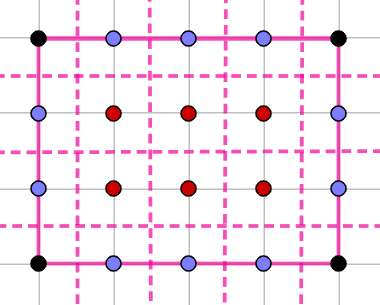
\includegraphics[width= 0.62\linewidth]{1}
		\caption{\small\textit{\color{toancuabi}Hình $1$.}}
		\vspace*{-5pt}
	\end{figure}
	Khi đó ta thấy
	\vskip 0.1cm
	-- Mỗi điểm nguyên ({\color{red}màu đỏ}) nằm trong hình chữ nhật ứng với một hình vuông đơn vị;
	\vskip 0.1cm
	-- Mỗi điểm nguyên ({\color{blue}màu xanh dương}) nằm trên các cạnh của hình chữ nhật mà không phải đỉnh ứng với một nửa hình vuông đơn vị;
	\vskip 0.1cm
	Mỗi điểm nguyên là đỉnh ({\color{black}màu đen}) của hình chữ nhật ứng với một phần tư hình vuông đơn vị.
	\vskip 0.1cm
	Như vậy
	\vskip 0.1cm
	Diện tích của hình chữ nhật $=$ số điểm trong hình chữ nhật
	$+ \dfrac{1}{2}\times$ số điểm trên cạnh mà không phải đỉnh $+ \dfrac{1}{4}\times$ số đỉnh
	\vskip 0.1cm
	Do hình chữ nhật có $4$ đỉnh nên ta thấy ngay
	\vskip 0.1cm
	Diện tích của hình chữ nhật $=$ số điểm trong hình chữ nhật 
	$+ \dfrac{1}{2} \times$ số điểm nằm trên cạnh
	$- 1$.
	\vskip 0.1cm
	Từ đó ta có diện tích của hình chữ nhật trên là:
	\begin{align*}
		6 + \frac{1}{2}\times14 - 1 = 12 \text{ (đơn vị diện tích).}
	\end{align*}
	Ví dụ trên được tính trong một trường hợp cụ thể, tuy nhiên những lập luận này hoàn toàn có thể áp dụng cho tất cả những hình chữ nhật khác cùng đặc điểm. Như vậy diện tích của hình chữ nhật có các cạnh trùng với những đường thẳng của lưới có thể được tính thông qua số điểm nguyên nằm trong và nằm trên cạnh của hình chữ nhật. Nếu ta gọi $T$ là số điểm nằm trong và $B$ là số điểm nằm trên các cạnh của hình chữ nhật, thì diện tích của hình chữ nhật là:
	\begin{align*}
		T+  \frac{B}{2} - 1.
	\end{align*}
	Một công thức thật đơn giản, thật hay đúng không các em. Không biết ngoài hình chữ nhật, công thức tính diện tích này còn đúng với những hình nào nữa nhỉ?
	\vskip 0.1cm
	Chúng ta cùng xem xét diện tích hình cơ bản thứ hai được đề cập trong Phần $1$ -- tam giác vuông có hai cạnh góc vuông trùng với những đường thẳng của lưới.
	\begin{figure}[H]
		\vspace*{-5pt}
		\centering
		\captionsetup{labelformat= empty, justification=centering}
		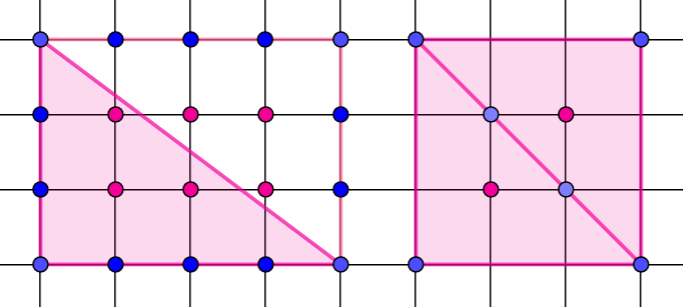
\includegraphics[width= 0.7\linewidth]{2}
		\caption{\small\textit{\color{toancuabi}Hình $2$.}}
		\vspace*{-10pt}
	\end{figure}
	Bây giờ ta kẻ hình chữ nhật bao quanh tam giác vuông và dùng công thức tính diện tích qua các điểm của hình chữ nhật được chỉ ra ở trên để xem về công thức tính diện tích của tam giác.
	\vskip 0.1cm
	Giả sử trên cạnh huyền của tam giác vuông có $d$ điểm nguyên. Nhận thấy $d$ điểm này vẫn là điểm trong của hình chữ nhật bao quanh. Do đó
	\vskip 0.1cm
	Số điểm trong $t$ của hình tam giác $= \dfrac{1}{2} \times $ (số điểm trong $T$ của hình chữ nhật $-$ số điểm trên cạnh huyền $d$)
	\vskip 0.1cm
	Hay $T = 2\times t + d$.
	\vskip 0.1cm
	Mặt khác, do tính đối xứng nên số điểm nguyên nằm trên hai cạnh góc vuông của tam giác vuông đã cho và tam giác vuông bù với nó, nên ta lại có
	\vskip 0.1cm
	Số điểm biên $b$ của hình tam giác $= \dfrac{1}{2} \times$ số điểm biên $B$ của hình chữ nhật 
	$+ 1$ điểm đỉnh $+$ số điểm trên cạnh huyền $d$.
	\vskip 0.1cm
	Hay $B = 2i - 2d - 2$.
	\vskip 0.1cm
	Vậy từ công thức tính diện tích của hình chữ nhật, ta có
	\vskip 0.1cm
	Diện tích tam giác vuông $= \dfrac{1}{2}$ diện tích hình chữ nhật
	$= \dfrac{T}{2} + \dfrac{B}{4} - \dfrac{1}{2}$
	$= t + \dfrac{b}{2} - 1$.
	\vskip 0.1cm
	Như vậy là công thức tính diện tích qua các điểm cũng đúng tiếp tam giác vuông! Đến đây, hẳn nhiều bạn nhỏ tiếp tục đặt câu hỏi: Công thức tính diện tích qua các điểm còn đúng cho dạng hình nào trên lưới nữa nhỉ? Câu hỏi này của chúng ta đã được một nhà toán học người Áo là Georg Alexander Pick ($1859 - 1942$) đưa ra câu trả lời. Ông đã chứng minh được Công thức tính diện tích qua những điểm nguyên đúng cho các đa giác đơn có các đỉnh là các điểm trên lưới. Kết quả này được phát biểu qua định lý mang tên ông -- Định lý Pick.
	\vskip 0.1cm
	\textbf{\color{toancuabi}Định lý Pick:} Cho một đa giác đơn có các đỉnh là các điểm nguyên của một lưới ô vuông. Giả sử có $T$ điểm nằm trong đa giác và $B$ điểm nằm trên các cạnh của đa giác (bao gồm cả các đỉnh). Khi đó diện tích của đa giác là:
	\begin{align*}
		T+  \dfrac{B}{2}-1.
	\end{align*}
	Một lưu ý là Định lý Pick tính diện tích cho những hình là đa giác đơn, là những đa giác không có cạnh tự cắt các em nhé. Dưới đây là một vài minh họa cho những đa giác loại này.
	\begin{figure}[H]
		\vspace*{-5pt}
		\centering
		\captionsetup{labelformat= empty, justification=centering}
		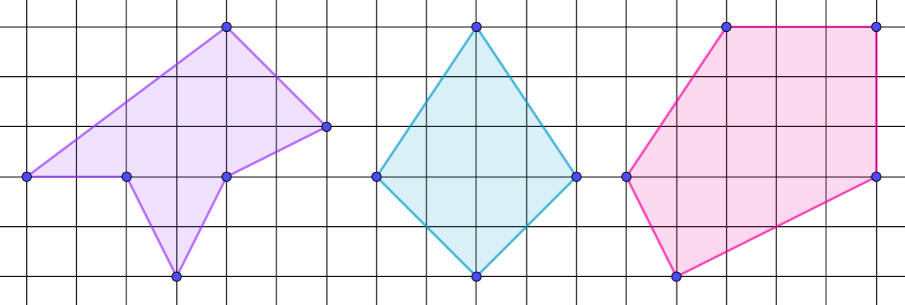
\includegraphics[width= 1\linewidth]{3}
		\caption{\small\textit{\color{toancuabi}Hình $3$. Đa giác đơn.}}
		\vspace*{-5pt}
	\end{figure}
	\begin{figure}[H]
		\vspace*{5pt}
		\centering
		\captionsetup{labelformat= empty, justification=centering}
		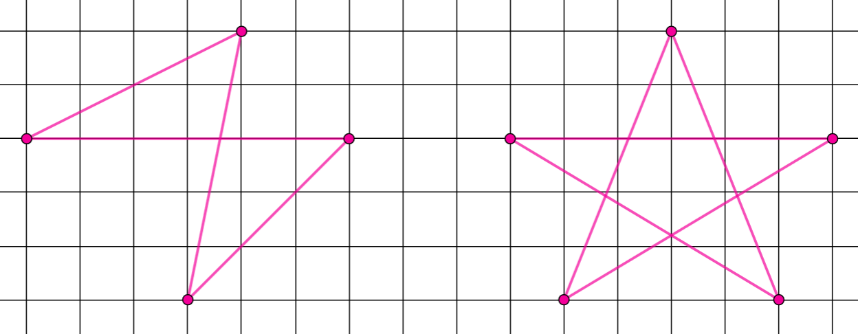
\includegraphics[width= 1\linewidth]{4}
		\caption{\small\textit{\color{toancuabi}Hình $4$. Đa giác không đơn.}}
		\vspace*{-10pt}
	\end{figure}
	Việc áp dụng định lý cho các đa giác không đơn có thể dẫn đến kết quả không chính xác. Các em ghi nhớ điều này khi dùng định lý Pick để tính diện tích nhé.
	\begin{figure}[H]
		\vspace*{-5pt}
		\centering
		\captionsetup{labelformat= empty, justification=centering}
		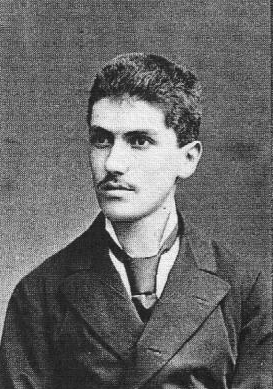
\includegraphics[width= 0.55\linewidth]{5}
		\caption{\small\textit{\color{toancuabi}Hình $5$. Georg Alexander Pick.}}
		\vspace*{-10pt}
	\end{figure}
	Định lý Pick được phát biểu đầy đủ như sau.
	\vskip 0.1cm
	$\pmb{2.}$ \textbf{\color{toancuabi}Tính diện tích theo định lý Pick}
	\vskip 0.1cm
	Trong mục này, chúng ta tính lại diện tích của một số hình trong Phần $1$ theo công thức có được từ định lý Pick và so sánh với nhau nhé.
	Đầu tiên là ``chú mèo" đáng yêu trong Ví dụ $4$ của Phần $1$.
	\vskip 0.1cm
	\textbf{\color{toancuabi}Ví dụ} $1$. Tính diện tích của hình được tô đậm dưới đây.
	\begin{figure}[H]
		\vspace*{-5pt}
		\centering
		\captionsetup{labelformat= empty, justification=centering}
		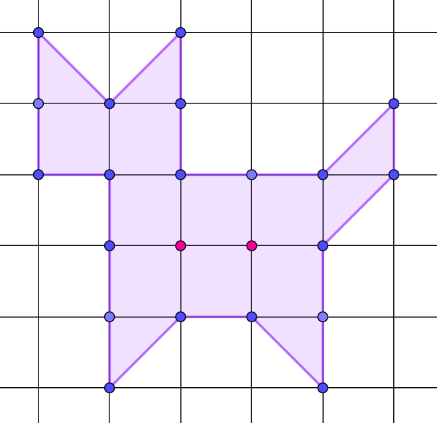
\includegraphics[width= 0.45\linewidth]{6}
		\caption{\small\textit{\color{toancuabi}Hình $6$.}}
		\vspace*{-10pt}
	\end{figure}
	\textit{Lời giải.} Ta dễ dàng thấy ngay $T = 2$ điểm trong ``chú mèo" và $B = 20$ điểm nằm trên các cạnh biên. Từ đó, diện tích của ``chú mèo" là:
	\begin{align*}
		T + \frac{B}{2} - 1 = 2 + \frac{20}{2} - 1 = 11 \text{ (đơn vị diện tích)}.
	\end{align*}
	Kết quả này cũng giống với con số mà ta đã tính được trong Phần $1$, nhưng có phần nhanh chóng hơn các em nhỉ.
	\vskip 0.1cm
	Chúng ta thử tiếp với hình trong Ví dụ $6$ trong Phần $1$.
	\vskip 0.1cm
	\textbf{\color{toancuabi}Ví dụ} $\pmb{2.}$ Tính diện tích của đa giác được tô đậm trong hình sau.
	\begin{figure}[H]
		\vspace*{-5pt}
		\centering
		\captionsetup{labelformat= empty, justification=centering}
		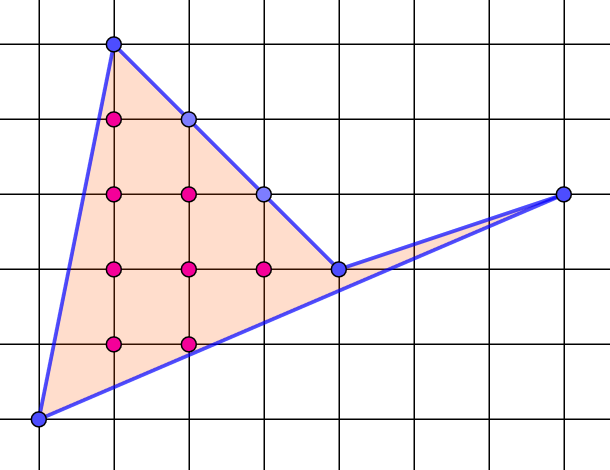
\includegraphics[width= 0.55\linewidth]{7}
		\caption{\small\textit{\color{toancuabi}Hình $7$.}}
		\vspace*{-10pt}
	\end{figure}
	\textit{Lời giải.}	Đa giác trong Hình $7$ có $T = 8$ điểm trong và $B = 6$ điểm nằm trên các canh. Do đó, Định lý Pick cho ta diện tích của đa giác này là:
	\begin{align*}
		T + \frac{B}{2} - 1 = 10 \text{ (đơn vị diện tích).}
	\end{align*}
	Kết quả này tất nhiên là trùng với con số tính ra theo cách giới thiệu ở Phần $1$ rồi, nhưng thay vì phải tính khá nhiều diện tích tam giác thông qua phương pháp lấy phần bù, chúng ta chỉ cần đếm số điểm nằm trên lưới. Định lý Pick thật là lợi hại phải không!
	\vskip 0.1cm
	Bài tập dưới đây để các em luyện tập thêm công thức Pick. Các em có thể tính diện tích theo cách trong Phần $1$ để kiểm tra lại nhé.
	\vskip 0.1cm
	\textbf{\color{toancuabi}Bài tập} $\pmb{1.}$ Tính diện tích của hình tô đậm sau đây.
	\begin{figure}[H]
		\vspace*{-5pt}
		\centering
		\captionsetup{labelformat= empty, justification=centering}
		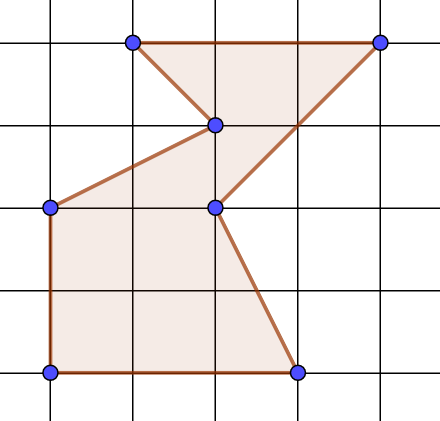
\includegraphics[width= 0.35\linewidth]{8}
		\caption{\small\textit{\color{toancuabi}Hình $8$.}}
		\vspace*{-5pt}
	\end{figure}
	$\pmb{3.}$ \textbf{\color{toancuabi}Làm thế nào để chứng minh định lý Pick?}
	\vskip 0.1cm
	Định lý Pick có thể chứng minh bằng nhiều cách khác nhau, trong khuôn khổ bài viết này, chúng ta chỉ mô tả cách tìm ra công thức của Pick cho hai hình cơ bản, đơn giản nhất -- hình chữ nhật và tam giác vuông có cạnh nằm trên lưới.
	\vskip 0.1cm 
	Nếu bạn nào quan tâm đến việc chứng minh đầy đủ định lý này thì có thể tham khảo các bước làm sau.
	\vskip 0.1cm
	-- Để chứng minh công thức Pick cho một đa giác nào đó ta chia đa giác thành hai phần bằng một đường chéo và quy về việc chứng công thức Pick cho mỗi đa giác thành phần. Ta thấy, đường chéo này trở thành cạnh của hai đa giác thành phần do đó các điểm nguyên trên đường chéo lúc trước được tính $1$ đơn vị, khi trở thành điểm biên thì tính $\dfrac{1}{2}$ đơn vị nhưng tính hai lần, vậy là hòa! Còn lại là hai điểm mút của đường chéo, chúng được tính hai lần do là đỉnh của hai đa giác con, vậy là dôi ra $1$ đơn vị. Nhưng trong công thức Pick sau khi tính các điểm biên và điểm trong ta bớt đi $1$ đơn vị. Đối với hai đa giác thành phần, ta bớt đi cả thảy $2$ đơn vị, vậy cũng hòa! 
	\begin{figure}[H]
		\vspace*{-5pt}
		\centering
		\captionsetup{labelformat= empty, justification=centering}
		
\includegraphics[width= 0.45\linewidth]{9}
		\caption{\small\textit{\color{toancuabi}Hình $9$.}}
		\vspace*{-10pt}
	\end{figure}
	-- Sau khi thực hiện nhiều lần chia đa giác thành các đa giác con, cuối cùng ta quy việc chứng minh định lý Pick cho tam giác. Ta lại tiếp tục chia tam giác đó thành các tam giác con nếu có một điểm nguyên ở trong hoặc trên biên tam giác. 
	\begin{figure}[H]
		\vspace*{5pt}
		\centering
		\captionsetup{labelformat= empty, justification=centering}
		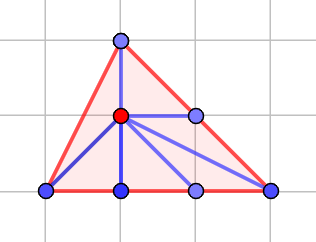
\includegraphics[width= 0.4\linewidth]{10}
		\caption{\small\textit{\color{toancuabi}Hình $10$.}}
		\vspace*{-10pt}
	\end{figure}
	-- Đối với tam giác không chứa điểm nguyên ở trong hoặc trên biên, định lý Pick khẳng định nó có diện tích bằng
	\begin{align*}
		\dfrac{3}{2}-1=\dfrac{1}{2} \text{ (đơn vị diện tích).}
	\end{align*}
	Dưới đây chúng ta sẽ xem một vài ví dụ kiểm chứng điều này. Hy vọng sau đó các bạn có thể tự đưa ra một chứng minh chặt chẽ của định lý Pick cho các tam giác đơn (nghĩa là tam giác không chứa điểm nguyên ở trong và trên biên, ngoại từ ba đỉnh).
	\begin{figure}[H]
		\vspace*{-5pt}
		\centering
		\captionsetup{labelformat= empty, justification=centering}
		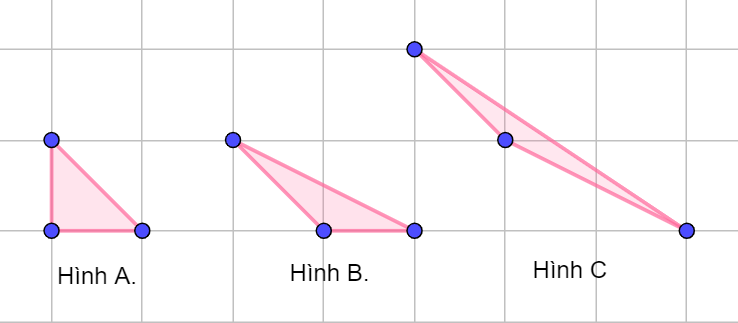
\includegraphics[width= 1\linewidth]{11}
		\caption{\small\textit{\color{toancuabi}Hình $11$.}}
		\vspace*{-10pt}
	\end{figure}
	Ba tam giác trong Hình $11$ đều là các tam giác đơn. Ba tam giác này có nhiều hình dáng khác nhau, nhưng ta đều thấy chúng có diện tích bằng $\dfrac{1}{2}$.
	Thật vậy, vận dụng những cách tính diện tích trong Phần $1$, ta có thể thấy ngay
	\begin{figure}[H]
		\vspace*{-5pt}
		\centering
		\captionsetup{labelformat= empty, justification=centering}
		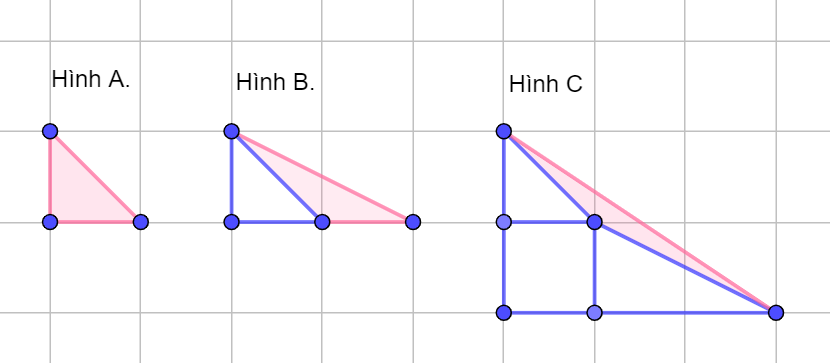
\includegraphics[width= 1\linewidth]{12}
		\caption{\small\textit{\color{toancuabi}Hình $12$.}}
		\vspace*{-10pt}
	\end{figure}
	-- Diện tích tam giác trong Hình $A$ là $\dfrac{1}{2}$;
	\vskip 0.1cm
	Diện tích của tam giác trong Hình $B$ là: 
	\begin{align*}
		\dfrac{1}{2}\times 1\times 2 - \dfrac{1}{2} = \dfrac{1}{2};
	\end{align*}
	Diện tích của tam giác trong Hình $C$ là: 
	\begin{align*}
		\dfrac{1}{2}\times2\times3 - \dfrac{1}{2} - 1 - \dfrac{1}{2}\times1\times2 = \dfrac{1}{2}.
	\end{align*}
	Bài viết về Tính diện tích trên lưới ô vuông đã giới thiệu đến các em cách tính diện tích của những hình trên lưới. Đầu tiên là hai phương pháp rất phổ biến: phương pháp chia hình cần tính thành những hình cơ bản đã biết diện tích và phương pháp tính theo phần bù. Tiếp theo đó bài viết giới thiệu với các em một công thức tính diện tích vô cùng đẹp đẽ qua Định lý Pick. Việc áp dụng định lý Pick giúp tính diện tích trở nên đơn giản hơn nhiều vì ta chỉ cần đếm số điểm nguyên ở trong và trên cạnh của hình cần tính. Chủ đề tính diện tích trên lưới ô vuông vẫn còn nhiều điều hấp dẫn, các bạn nhỏ nếu tìm được những bài toán hay thì hãy chia sẻ cùng Pi và các thầy cô trong câu lạc bộ UMC nhé.
\end{multicols}
\vspace*{-10pt}
{\color{toancuabi}\rule{1\linewidth}{0.1pt}}
\blfootnote{\color{toancuabi}$^1$THPT Chuyên Hưng Yên.}
\begingroup
\AddToShipoutPicture*{\put(126,452){
\includegraphics[scale=1]{../tieude10.pdf}}}
\centering
\endgroup
\vspace*{66pt}
\begin{multicols}{2}
	Các quốc gia trên thế giới có nhiều hình thức tổ chức đón năm mới khác nhau, trong đó phải kể đến việc phát hành tem bưu chính. Tem của các nước phương Tây gắn liền với dịp lễ Giáng sinh và ngày đầu năm mới. Phương Đông đón Tết theo lịch mặt trăng vì thế tem Tết các nước châu Á mang nhiều ý nghĩa văn hóa phương Đông. Đối với người xa Tổ quốc, mỗi khi nhận được lá thư hoặc bưu thiếp dán tem Tết lại gợi nhớ quê hương, cội nguồn, nhớ về ngày Tết cổ truyền của dân tộc mình và con tem cũng là hàm ý như lời chúc mừng năm mới từ người gửi đến người nhận. Lời chúc qua thư và bưu thiếp có tem Tết mang nét độc đáo riêng mà lời chúc qua hệ thống liên lạc khác không dễ thay thế. Tem như một lời nhắn gửi Tết là thời khắc thiêng liêng để vạn vật được hồi sinh, để những người con xa quê hương có cơ hội đoàn tụ bên gia đình, cùng nhau đón thời khắc giao thừa với mong ước những điều may mắn, hạnh phúc, bình an, tài lộc sẽ đến trong năm mới. Tem Tết được phát hành hàng năm như lời chúc về một năm mới trăm điều an khang, vạn điều may mắn, mã đáo thành công, lộc đến nhà nhà.
	\vskip 0.1cm 
	Một trong những chủ đề không thể thiếu trên tem Tết ở các nước châu Á là hình tượng $12$ con giáp. Tính theo cung hoàng đạo, năm mới gắn với con vật nào thì con vật đó được các họa sĩ thể hiện trên tem để tôn vinh vẻ đẹp và ý nghĩa của nó như một linh vật trong năm. Tháng $8$ năm $1998$ tại hội thảo quốc tế về tem thư tổ chức tại Israel, tem $12$ con giáp được bầu chọn là đề tài đứng thứ $2$ trong bảng xếp hạng $10$ đề tài tem thư lưu hành phổ biến nhất trên thế giới. Điều này cho thấy văn hóa mười hai con giáp của phương Đông đã có sức hấp dẫn lôi cuốn những khu vực khác trên thế giới.
	\vskip 0.1cm 
	Hiện nay, có khoảng $80$ nước và các vùng lãnh thổ ở châu Á, châu Phi, châu Mỹ phát hành những bộ tem về động vật liên quan đến $12$ con giáp. Nước đầu tiên phát hành tem về các con giáp là Nhật Bản, tiếp đến là Hàn Quốc và Trung Quốc. Tết cổ truyền là một trong những dịp lễ trọng đại nhất trong năm ở Việt Nam, đóng vai trò rất quan trọng trong đời sống tinh thần của người Việt. Tem phát hành dịp Tết ở Việt Nam, cùng chung dòng chảy với văn hóa phương Đông nhưng nó được tiếp nhận, chắt lọc, sáng tạo biến cách trên nền tảng bản sắc dân tộc Việt. Tem Tết đầu tiên về con giáp ở Việt Nam được phát hành vào ngày $16$ tháng $1$ năm $1962$ với mẫu tem Tranh Tết Đông Hồ gồm hai mẫu \textit{Lợn lái, lợn con} và \textit{Gà mái, gà con} đều dựa theo tranh khắc gỗ dân gian Đông Hồ, một loại hình truyền thống dân tộc. 
	\begin{figure}[H]
		\vspace*{-5pt}
		\centering
		\captionsetup{labelformat= empty, justification=centering}
		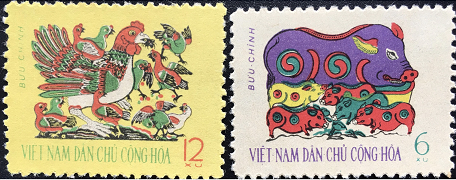
\includegraphics[width= 1\linewidth]{tem1}
		\vspace*{-15pt}
	\end{figure}
	Chuẩn bị bước sang năm mới Quý Mão ngày $1.12.2022$  Bộ Thông tin và Truyền thông phát hành bộ tem bưu chính “Tết Quý Mão” gồm $2$ mẫu tem và $1$ blốc do họa sĩ Nguyễn Quang Vinh thiết kế. Con Mèo trên tem được thể hiện theo phong cách hiện đại, đường nét dứt khoát, mạnh mẽ nhưng cũng thể hiện sự mềm mại, uyển chuyển. 
	\begin{figure}[H]
		\vspace*{-5pt}
		\centering
		\captionsetup{labelformat= empty, justification=centering}
		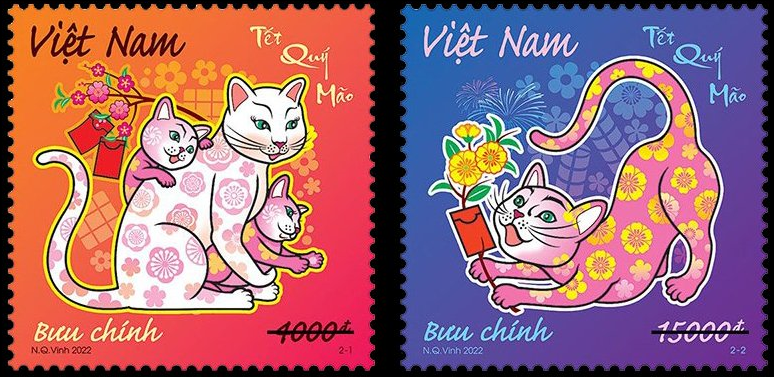
\includegraphics[width= 1\linewidth]{tem2}
		\vspace*{-15pt}
	\end{figure}
	Ở trung tâm mẫu tem thứ nhất là hình ảnh mèo mẹ và hai chú mèo con đang quấn quýt, vui đùa. Mèo mẹ ôm và cõng mèo con trên lưng cũng như biết bao người mẹ trên cuộc đời: vừa bao dung ôm trọn con vào lòng, bảo vệ con trước giông tố, sóng gió; vừa sẵn sàng "cõng" con, cùng con vượt bao khó khăn, vất vả trong cuộc sống. Hình ảnh mèo cha ở mẫu tem thứ hai được khắc họa trên nền tem màu xanh sắc lạnh, tạo liên tưởng đến hình ảnh người cha đầy mạnh mẽ, có phần "đơn độc", một mình gánh vác cả "thế giới" trên lưng để bảo vệ sự bình yên cho gia đình nhỏ của mình. Các chú mèo trong hai mẫu tem được sắp xếp đối xứng, hướng vào nhau như mong ước về đoàn viên, sum vầy ngày Tết được thể hiện trên mẫu blốc tem. Khung cảnh ấm áp của gia đình mèo gợi cho người xem một nỗi nhớ nhung, như thúc giục mọi người hãy nhanh nhanh sắp xếp công việc, bắt chuyến tàu Tết để về với gia đình, bởi ở đó mới thực sự là khung trời bình yên, để ta yên tâm bỏ lại những bộn bề, lo âu của cuộc sống và tận hưởng những phút giây hạnh phúc bên người thân yêu.
	\begin{figure}[H]
		\vspace*{-5pt}
		\centering
		\captionsetup{labelformat= empty, justification=centering}
		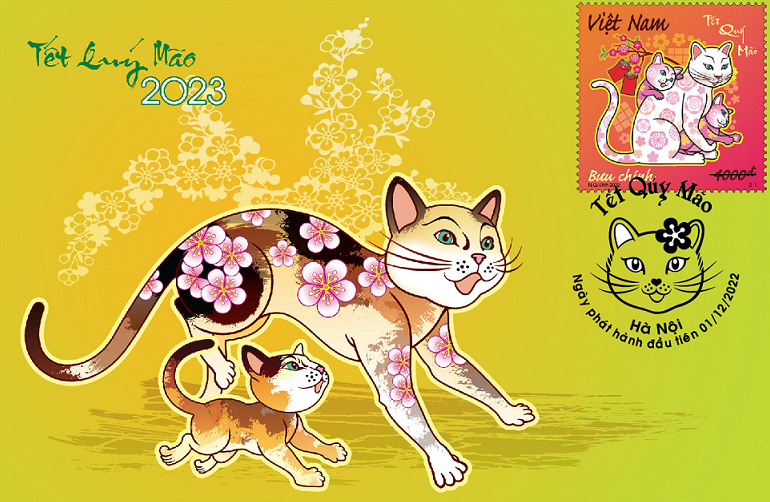
\includegraphics[height=0.382\linewidth]{tem3}
		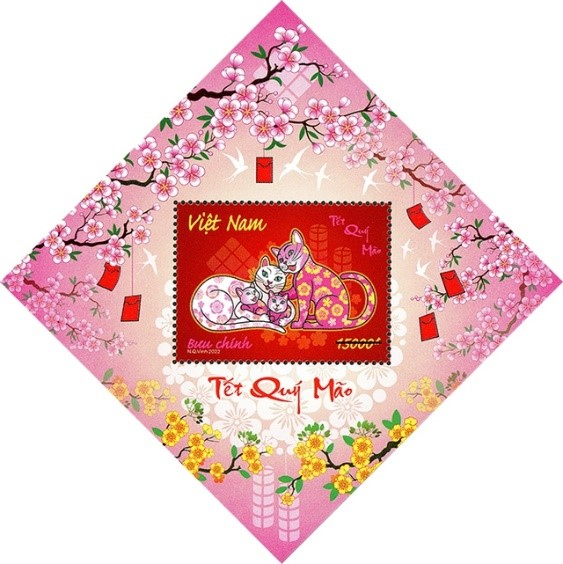
\includegraphics[height=0.382\linewidth]{tem4}
		\vspace*{-10pt}
	\end{figure}
	Các hình ảnh quen thuộc của ngày Tết như hoa đào, hoa mai, bánh chưng, bánh dày và bao lì xì đỏ cũng được thể hiện trên bloc. Đàn chim én tung bay được khắc họa trên nền blốc tem báo hiệu một năm mới rộn ràng, đầy hứa hẹn sắp đến. 
	\vskip 0.1cm
	Với các bạn đọc nhỏ tuổi của Pi, chúng ta hãy cùng thử sức với một số bài toán về tem sau đây nhé.
	\vskip 0.1cm
	\textbf{\color{toancuabi}Bài toán} $\pmb{1.}$ Có bao nhiêu cách dán $3$ tem thư khác nhau lên $3$ bì thư khác nhau?
	\vskip 0.1cm
	\textit{Lời giải.} Trước hết sắp xếp ba con tem theo thứ tự nào đó và lần lượt dán chúng:
	\vskip 0.1cm
	$\circ$	Chọn một bì thư để dán con tem thứ nhất: ta có $3$ cách làm như vậy.
	\vskip 0.1cm
	$\circ$	Chọn một bì thư trong số hai bì còn lại để dán tem thư thứ hai: ta có $2$ cách làm như vậy.
	\vskip 0.1cm
	$\circ$	Dán tem thư cuối cùng lên bì thư còn lại: ta  có $1$ cách làm.
	\vskip 0.1cm
	Do đó số cách dán ba tem thư khác nhau lên ba bì thư khác nhau là
%	\setlength{\abovedisplayskip}{7pt}
%	\setlength{\belowdisplayskip}{7pt}
	\begin{align*}
		3 \times 2 \times 1= 6 \text{ (cách).}
	\end{align*}
	\textbf{\color{toancuabi}Bài toán} $\pmb{2.}$ Minh thích chơi tem, bạn ấy đã sưu tầm được $450$ tem, được chia ra thành cách loại như sau: có $70$ tem phát hành ở các nước châu Mỹ, $210$ tem phát hành ở các nước châu Á và số tem còn lại được phát hành ở các nước châu Phi. Minh muốn chia đều mỗi loại tem phát hành ở các châu lục đó để ép vào các album tem. Hỏi có bao nhiêu cách chia với số album nhiều hơn $1$ (hai cách chia là như nhau nếu số tem mỗi loại trong một album là bằng nhau)? Số album cần có để mỗi album có số tem ít nhất là bao nhiêu? Tính số tem mỗi loại trong các album trong mỗi cách chia đó.
	\vskip 0.1cm
	\textit{Lời giải.}
	Số tem được phát hành ở các nước châu Phi là:
	\begin{align*}
		450 - 70 - 210 =170  \text{ (tem).}
	\end{align*}
	Gọi số album là $x$  ($x \in \mathbb{N^*}$).
	\vskip 0.1cm
	Ta có:
	\begin{align*}
		&70\,\,\vdots\,\, x, 210\,\,\vdots\,\, x; 170 \,\,\vdots\,\, x\\
		\Rightarrow & x \in  \text{ƯC}(70,210,170), 
	\end{align*}
	mà
	\begin{align*}
		&\text{ƯCLN}(70,210,170)=10 \\
		\Rightarrow &x \in \text{Ư}(10)=\{1,2,5,10\}
	\end{align*}
	Do đó số cách chia tem với số album nhiều hơn $1$ sẽ là $3$ cách: cách $1$ dùng $2$ album, cách $2$ dùng $5$ album và cách thứ ba dùng $10$ album.  
	Để số tem trong mỗi album là ít nhất thì Minh cần dùng số album là lớn nhất có thể, có nghĩa là Minh cần $10$ album.
	\vskip 0.1cm
	Nếu chia thành $2$ album thì số tem trong mỗi album là  $450 : 2 = 225$
	\vskip 0.1cm  
	Nếu chia thành $5$ album thì số tem trong mỗi album là $450:5=90$ 
	\vskip 0.1cm
	Nếu chia thành $10$ album thì số tem trong mỗi album là $450:10 = 45$
	\vskip 0.1cm 
	\textbf{\color{toancuabi}Bài toán} $\pmb{3.}$ Anh Hưng là nhà sưu tập tem và có nhiều bạn cùng sở thích. Dịp Tết Nhâm Dần, Bộ Thông tin và Truyền thông phát hành bộ tem bưu chính gồm $2$ mẫu tem và $1$ blốc với giá lần lượt $4$ nghìn đồng, $15$ nghìn đồng và $38$ nghìn đồng. Anh Hưng đến Bưu điện thành phố mua để tặng bạn bè những sản phẩm mới đó với $600$ nghìn đồng. Anh muốn số tem loại $4$ nghìn đồng gấp $10$ lần số blốc và dung hết số tiền để mua tem $15$ nghìn đồng”. Theo bạn thì Hưng nhận được bao nhiêu chiếc cho mỗi loại tem và blốc? 
	\vskip 0.1cm
	\textit{Lời giải.}
	Gọi $x$ là số blốc, $y$ là số tem loại $15$ nghìn đồng. Khi đó số tem loại $4$ nghìn đồng là $10x$  ($x, y \in \mathbb{N^*}$)
	\vskip 0.1cm
	Khi đó  $10x \cdot 4 +15\cdot y +38\cdot y =600$. Từ đó 
	\begin{align*}
		78x + 15y = 600. \tag{$1$}
	\end{align*}
	Ta có  $78x = 600 - 15y = 15(40-y)$. Suy ra $78x < 600$  và $78x$ chia hết cho $5$. Từ đó, ta có  $x < 8$ và do đó $x = 5$. Thay vào phương trình ($1$) ta thu được $78 \cdot 5 + 15y = 600$, dẫn đến $15y = 210$ và vì thế $y = 14$.
	\vskip 0.1cm
	Như vậy, anh Hưng nhận được $50$ tem loại $4$ nghìn đồng, $14$ tem loại $15$ nghìn đồng và $5$ blốc giá $38$ nghìn đồng.
	\vskip 0.1cm
	Cuối cùng mời các bạn đọc nhỏ tuổi thử sức với hai bài toán sau.
	\vskip 0.1cm
	\textbf{\color{toancuabi}Bài} $\pmb{1.}$ Hai bạn Minh và Hải chơi tem thư. Nếu Minh cho Hải một số tem bằng số con tem mà Hải sưu tầm được, rồi Hải lại cho Minh một số tem bằng số tem còn lại của Minh thì kết quả là Minh sẽ có số tem nhiều hơn số mà Minh đã sưu tầm được là $30$ con tem và khi đó Hải có số tem bằng một phần ba lần số tem mà Hải sưu tầm được. Hỏi số tem mà mỗi bạn đã sưu tầm được là bao nhiêu?
	\vskip 0.1cm
	\textbf{\color{toancuabi}Bài} $\pmb{2.}$ Có $3$ tem thư khác nhau và $6$ bì thư cũng khác nhau. Hỏi có bao nhiêu cách dán $3$ tem thư lên $3$ trong $6$ bì thư đó ?
\end{multicols}
\newpage
\begingroup
\AddToShipoutPicture*{\put(121,650){
\includegraphics[scale=1]{../tieude.pdf}}} 
\centering
\endgroup
\vspace*{52pt}
\begin{multicols}{2}
	Thám tử Xuân Phong và thanh tra Lê Kính nhân dịp đi điều tra ở vùng xa được mời tới thăm quan một thành phố kỳ lạ được mang tên Thành phố Thông minh. Thành phố chỉ có vẻn vẹn $200$ cư dân, họ ở trong những ngôi nhà cực kỳ hiện đại với nhiều tiện nghi tối tân và đặc biệt hơn, cư dân được chia ra thành $3$ loại người: $a)$ Người \textit{ngốc ngếch} luôn coi tất cả mọi người khác là ngốc ngếch còn mỗi mình là thông minh; $b)$ người \textit{thông minh khiêm tốn} biết chính xác về tất cả những người khác, còn coi bản thân là ngốc ngếch; $c)$ người \textit{thông minh tự tin} biết chính xác về tất cả những người khác và coi mình là thông minh. Theo thói quen nghề nghiệp, Xuân Phong liền mời tất cả công dân của thành phố tới tòa thị chính để mở một cuộc điều tra khảo sát ẩn danh về câu hỏi: trong tòa thị chính bây giờ có tất cả bao nhiêu công dân của thành phố là thông minh? Sau khi thu phiếu điều tra về, Xuân Phong không thể nào xác định được số lượng công dân thông minh của thành phố. Bỗng dưng vừa đúng lúc đó có một công dân trở về sau chuyến du lịch và chưa kịp tham gia trả lời khảo sát cùng với $199$ công dân đứng chật ních ở tòa thị chính. Anh ta nhanh chóng nhận phiếu điều tra, điền thông tin về các công dân trong phòng thị chính, kể cả về bản thân. Xuân Phong đọc câu trả lời của công dân đến muộn này và nói nhỏ cho Lê Kính “Giờ thì tôi cũng biết rõ về số các nhà thông minh trong thành phố này rồi”.
	\vskip 0.1cm
	Vậy theo em trong thành phố đặc biệt nọ có thể có bao nhiêu công dân thông minh?
	\begin{figure}[H]
		\centering
		\vspace*{-10pt}
		\captionsetup{labelformat= empty, justification=centering}
		\includegraphics[width=1\linewidth]{Pi1_2_XuanPhong}
		\vspace*{-5pt}
	\end{figure}	
	%	Tất cả các người \textit{ngốc ngếch} đều trả lời “Một”. Nếu trong tòa thị chính  có ít nhất là $3$ công dân thông minh, thì tất cả họ sẽ đưa ra một số không nhỏ hơn $2$, và Xuân Phong đã biết được ngay câu trả lời. Vì thế, số công dân thông minh chỉ có thể là $0$, $1$ hoặc $2$. Ta xét tất cả các trường hợp.
	%	\vskip 0.1cm
	%	Nếu không có công dân thông mình nào, thì tất cả sẽ trả lời là “Một”. Nếu chỉ có một công dân thông minh và hơn nữa lại tự tin, thì anh ta cũng trả lời “Một” và tình huống này không phân biệt được với tình huống trước. Nếu người thông minh duy nhất là khiêm tốn, thì anh ta sẽ trả lời “Không có ai”, và trường hợp này phân biệt được ngay.
	%	\vskip 0.1cm
	%	Nếu có hai công dân thông minh và lại khiêm tốn, thì họ cũng lại trả lời “Một”, và tình huống này không phân biệt được với tình huống thứ nhất. Còn nếu có hai công dân thông minh và cả hai lại tự tin, thì họ sẽ đều trả lời “Hai”, tình huống này phân biệt được rõ ngay. Còn nếu có một công dân thông minh tự tin và một công dân thông minh khiêm tốn, thì người thông minh tự tin cũng trả lời “Hai” và tình huống phân biệt được.
	%	\vskip 0.1cm
	%	Như vậy, chỉ có thể có $3$ trường hợp không phân biệt được rõ ràng khi khảo sát $199$ công dân: không có công dân thông minh nào, có một người thông minh tự tin, và có hai người thông minh khiêm tốn. Trong cả $3$ phương án này tất cả các phiếu điều tra đều ghi “Một”.
	%	\vskip 0.1cm
	%	Giờ ta sẽ xem, người tới muộn sẽ đưa ra những câu trả lời nào trong mỗi tình huống được nêu ở trên, phụ thuộc vào mức độ thông minh và khiêm tốn của anh ta.
	%	\vskip 0.1cm
	%	\begin{table}[H]
		%		\vspace*{-5pt}
		%		\centering
		%		\captionsetup{labelformat= empty, justification=centering}
		%		\begin{tabular}{|l|c|c|c|}
			%			\hline
			%			& $0$ người thông minh tự tin
			%			$0$ người thông minh khiêm tốn&	$1$ người thông minh tự tin
			%			$0$ người thông minh khiêm tốn&	$0$ người thông minh tự tin
			%			$2$ người thông minh khiêm tốn\\
			%			\hline
			%			Ngốc ngếch &	$1$&	$1$&	$1$\\
			%			\hline
			%			Tự tin	&$1$ &	$2$&	$3$\\
			%			\hline
			%			Khiêm tốn&	$0$&	$1$&	$2$\\
			%			\hline
			%		\end{tabular}
		%		\vspace*{-10pt}
		%	\end{table}
	%	Ta thấy rõ ràng là các câu trả lời “$1$” và “$2$” đều được gặp ở vài ô, có nghĩa là chúng không giúp gì được cho việc phân biệt các tình huống. Tuy nhiên các trả lời “$0$” và “$3$”
	%	lại gặp đúng một lần, và chúng cho phép đưa ra các kết luận duy nhất. Vì thế người tới muộn đã đưa ra một trong các câu trả lời đó. Trong trường hợp anh ta trả lời “$0$”
	%	thì trong thành phố có duy nhất $1$ công dân thông minh (là chính người tới muộn đó), còn trong trường hợp anh ta trả lời “$3$” thì đúng là trong thành phố có $3$ công dân thông minh ($2$ người khiêm tốn và $1$ người tự tin là anh tới muộn đó).
	%	\vskip 0.1cm
	%	Đáp số: $1$ hoặc $3$.
\end{multicols}
\vspace*{-20pt}
{\color{toancuabi}\rule{1\linewidth}{0.1pt}}
\begingroup
\AddToShipoutPicture*{\put(115,205){
\includegraphics[scale=0.98]{../tieude11.pdf}}} 
\centering
\endgroup
\vspace*{38pt}

\begin{multicols}{2}
	$\pmb{1.}$ Một bác nông dân chở một xe ô tô quất cảnh ra chợ Tết để bán. Sau khi bán hết cây quất cuối cùng với giá $230$ nghìn đồng, bác tính nhẩm lại thấy mình đã bán số cây quất với giá trung bì nh là $245$ nghìn đồng/cây. Nhưng ngay lúc ấy người mua cây quất cuối quay trở lại và chỉ cho bác thấy cành quất bị rụng quá nhiều lá, nên ông ta chỉ đồng ý mua với giá $158$ nghìn đồng. 
	\begin{figure}[H]
		\centering
		\vspace*{5pt}
		\captionsetup{labelformat= empty, justification=centering}
		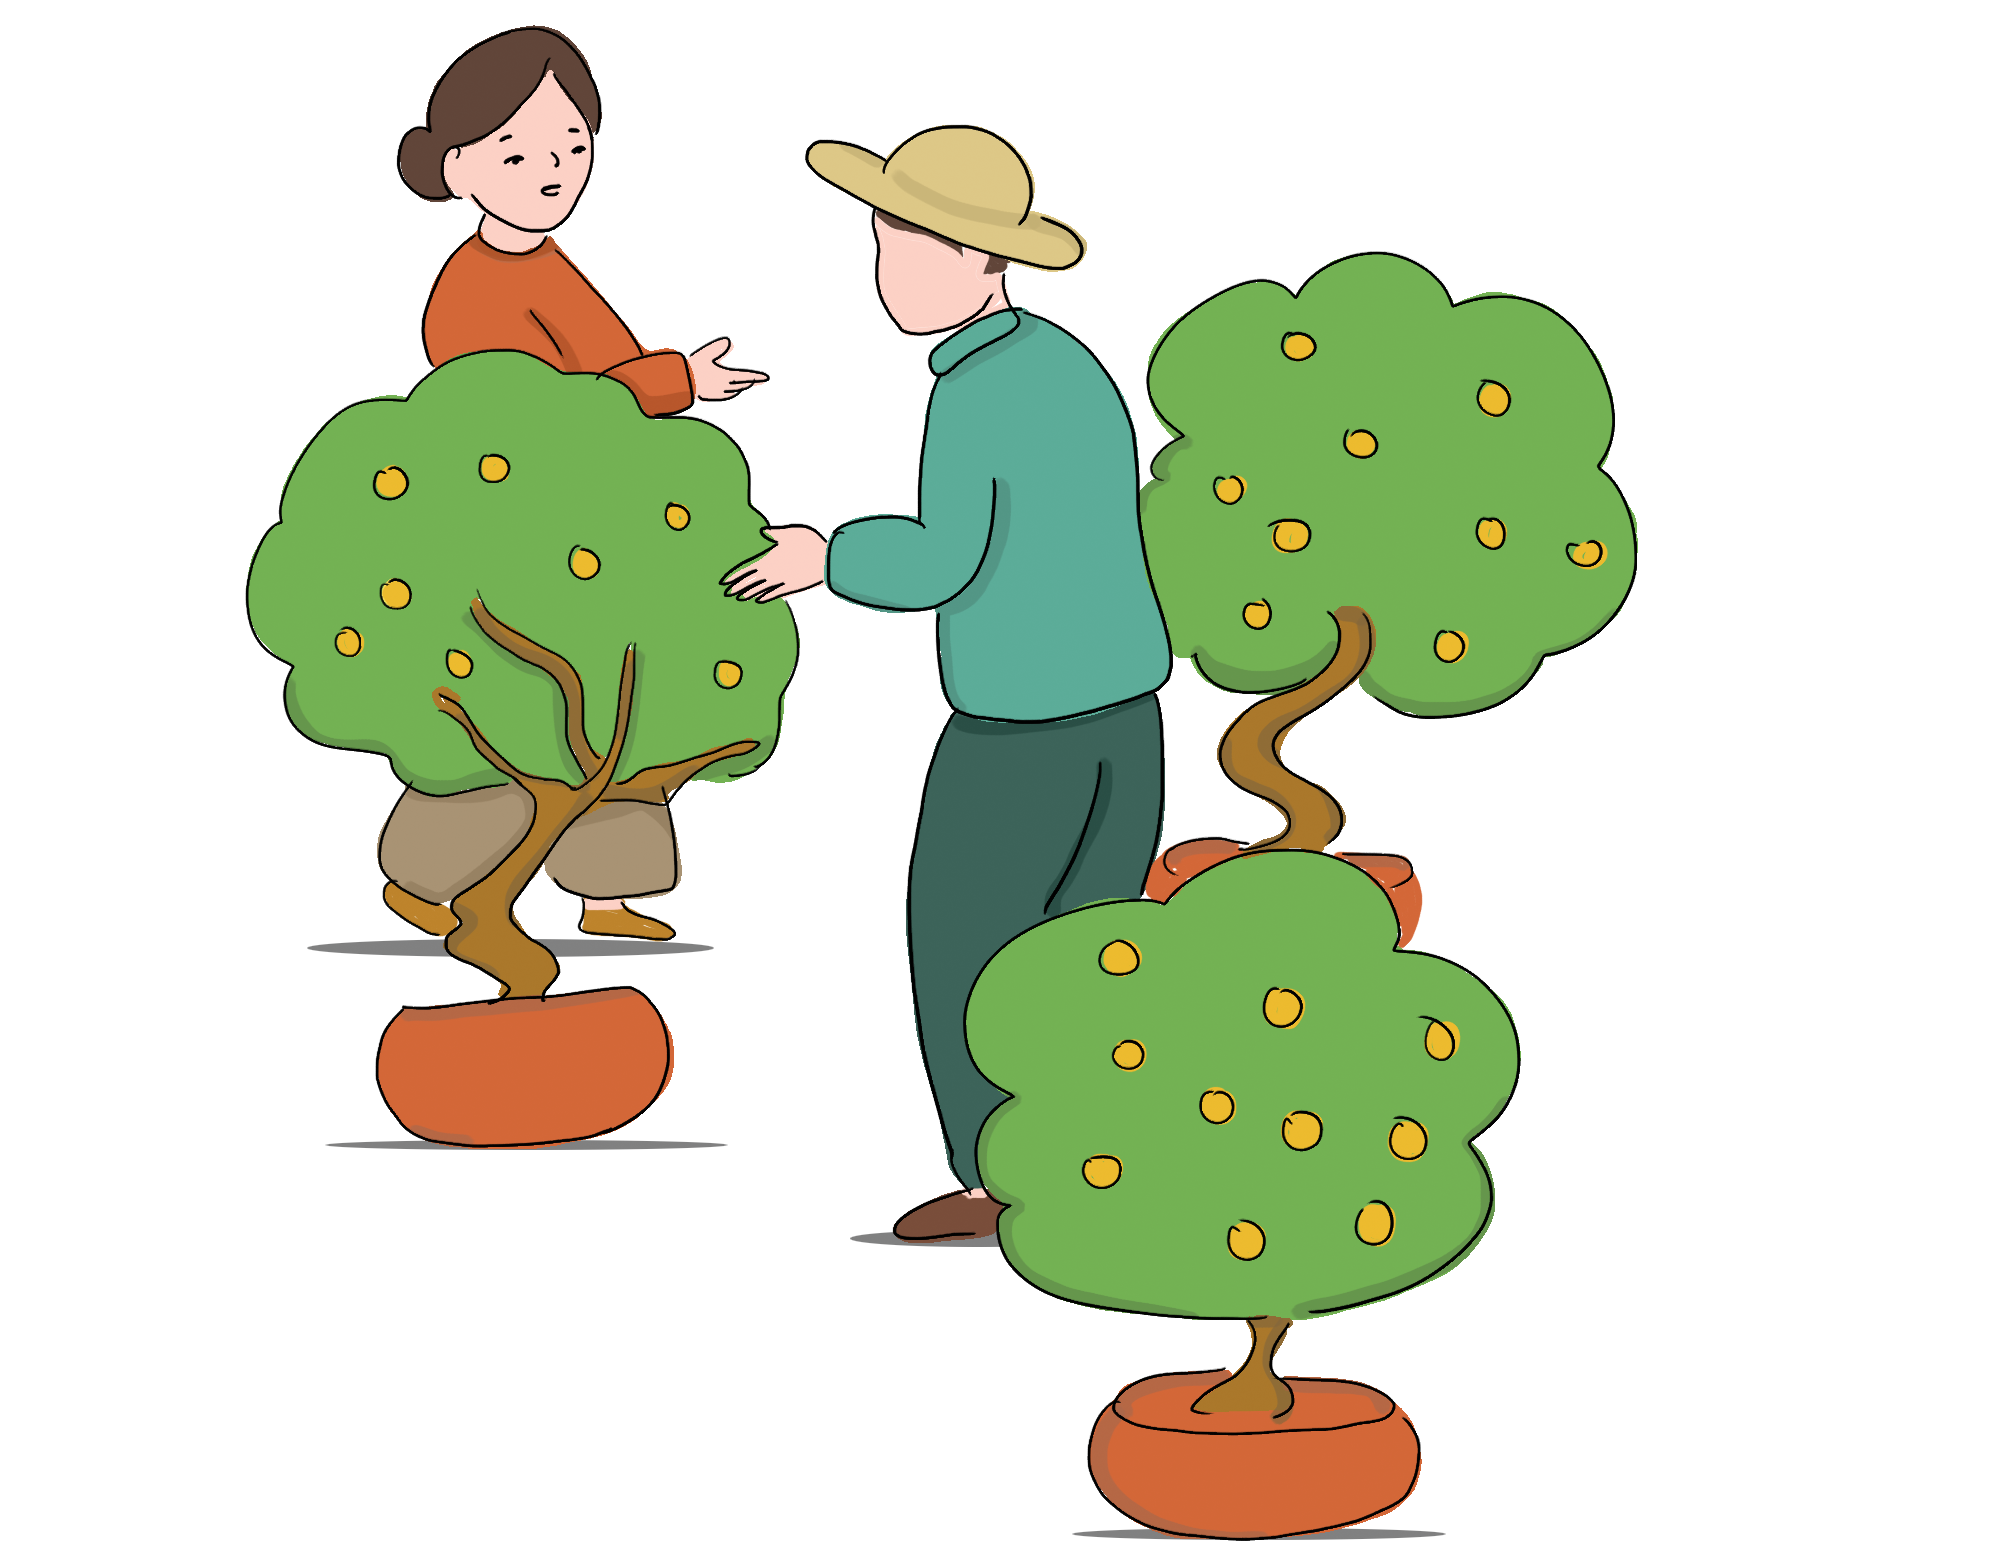
\includegraphics[width=0.8\linewidth]{Pi1_2_Bai1}
		\vspace*{-5pt}
	\end{figure}
	Bác chấp thuận và bán cây quất đó. Khi nhẩm tính lại, bác nông dân thấy giá trung bình của xe quất bây giờ là $242$ nghìn đồng. Hỏi bác đã bán được bao nhiêu cây quất?
	\vskip 0.1cm
	$\pmb{2.}$ Chuyện kể rằng có một người khi gặp nhà triết học và toán học Hy--lạp Pythagoras đã hỏi ông: “Bây giờ là mấy giờ?” Pythagoras đã trả lời “Cho đến hết ngày, còn lại hai lần của hai phần năm khoảng thời gian đã trôi qua từ lúc bắt đầu ngày”. Nghe vậy, người đó chịu không thể nghĩ ra ngay được lúc họ gặp nhau là mấy giờ. Em có thể giúp trả lời lúc đó là mấy giờ được không?
	\begin{figure}[H]
		\centering
		\vspace*{-5pt}
		\captionsetup{labelformat= empty, justification=centering}
		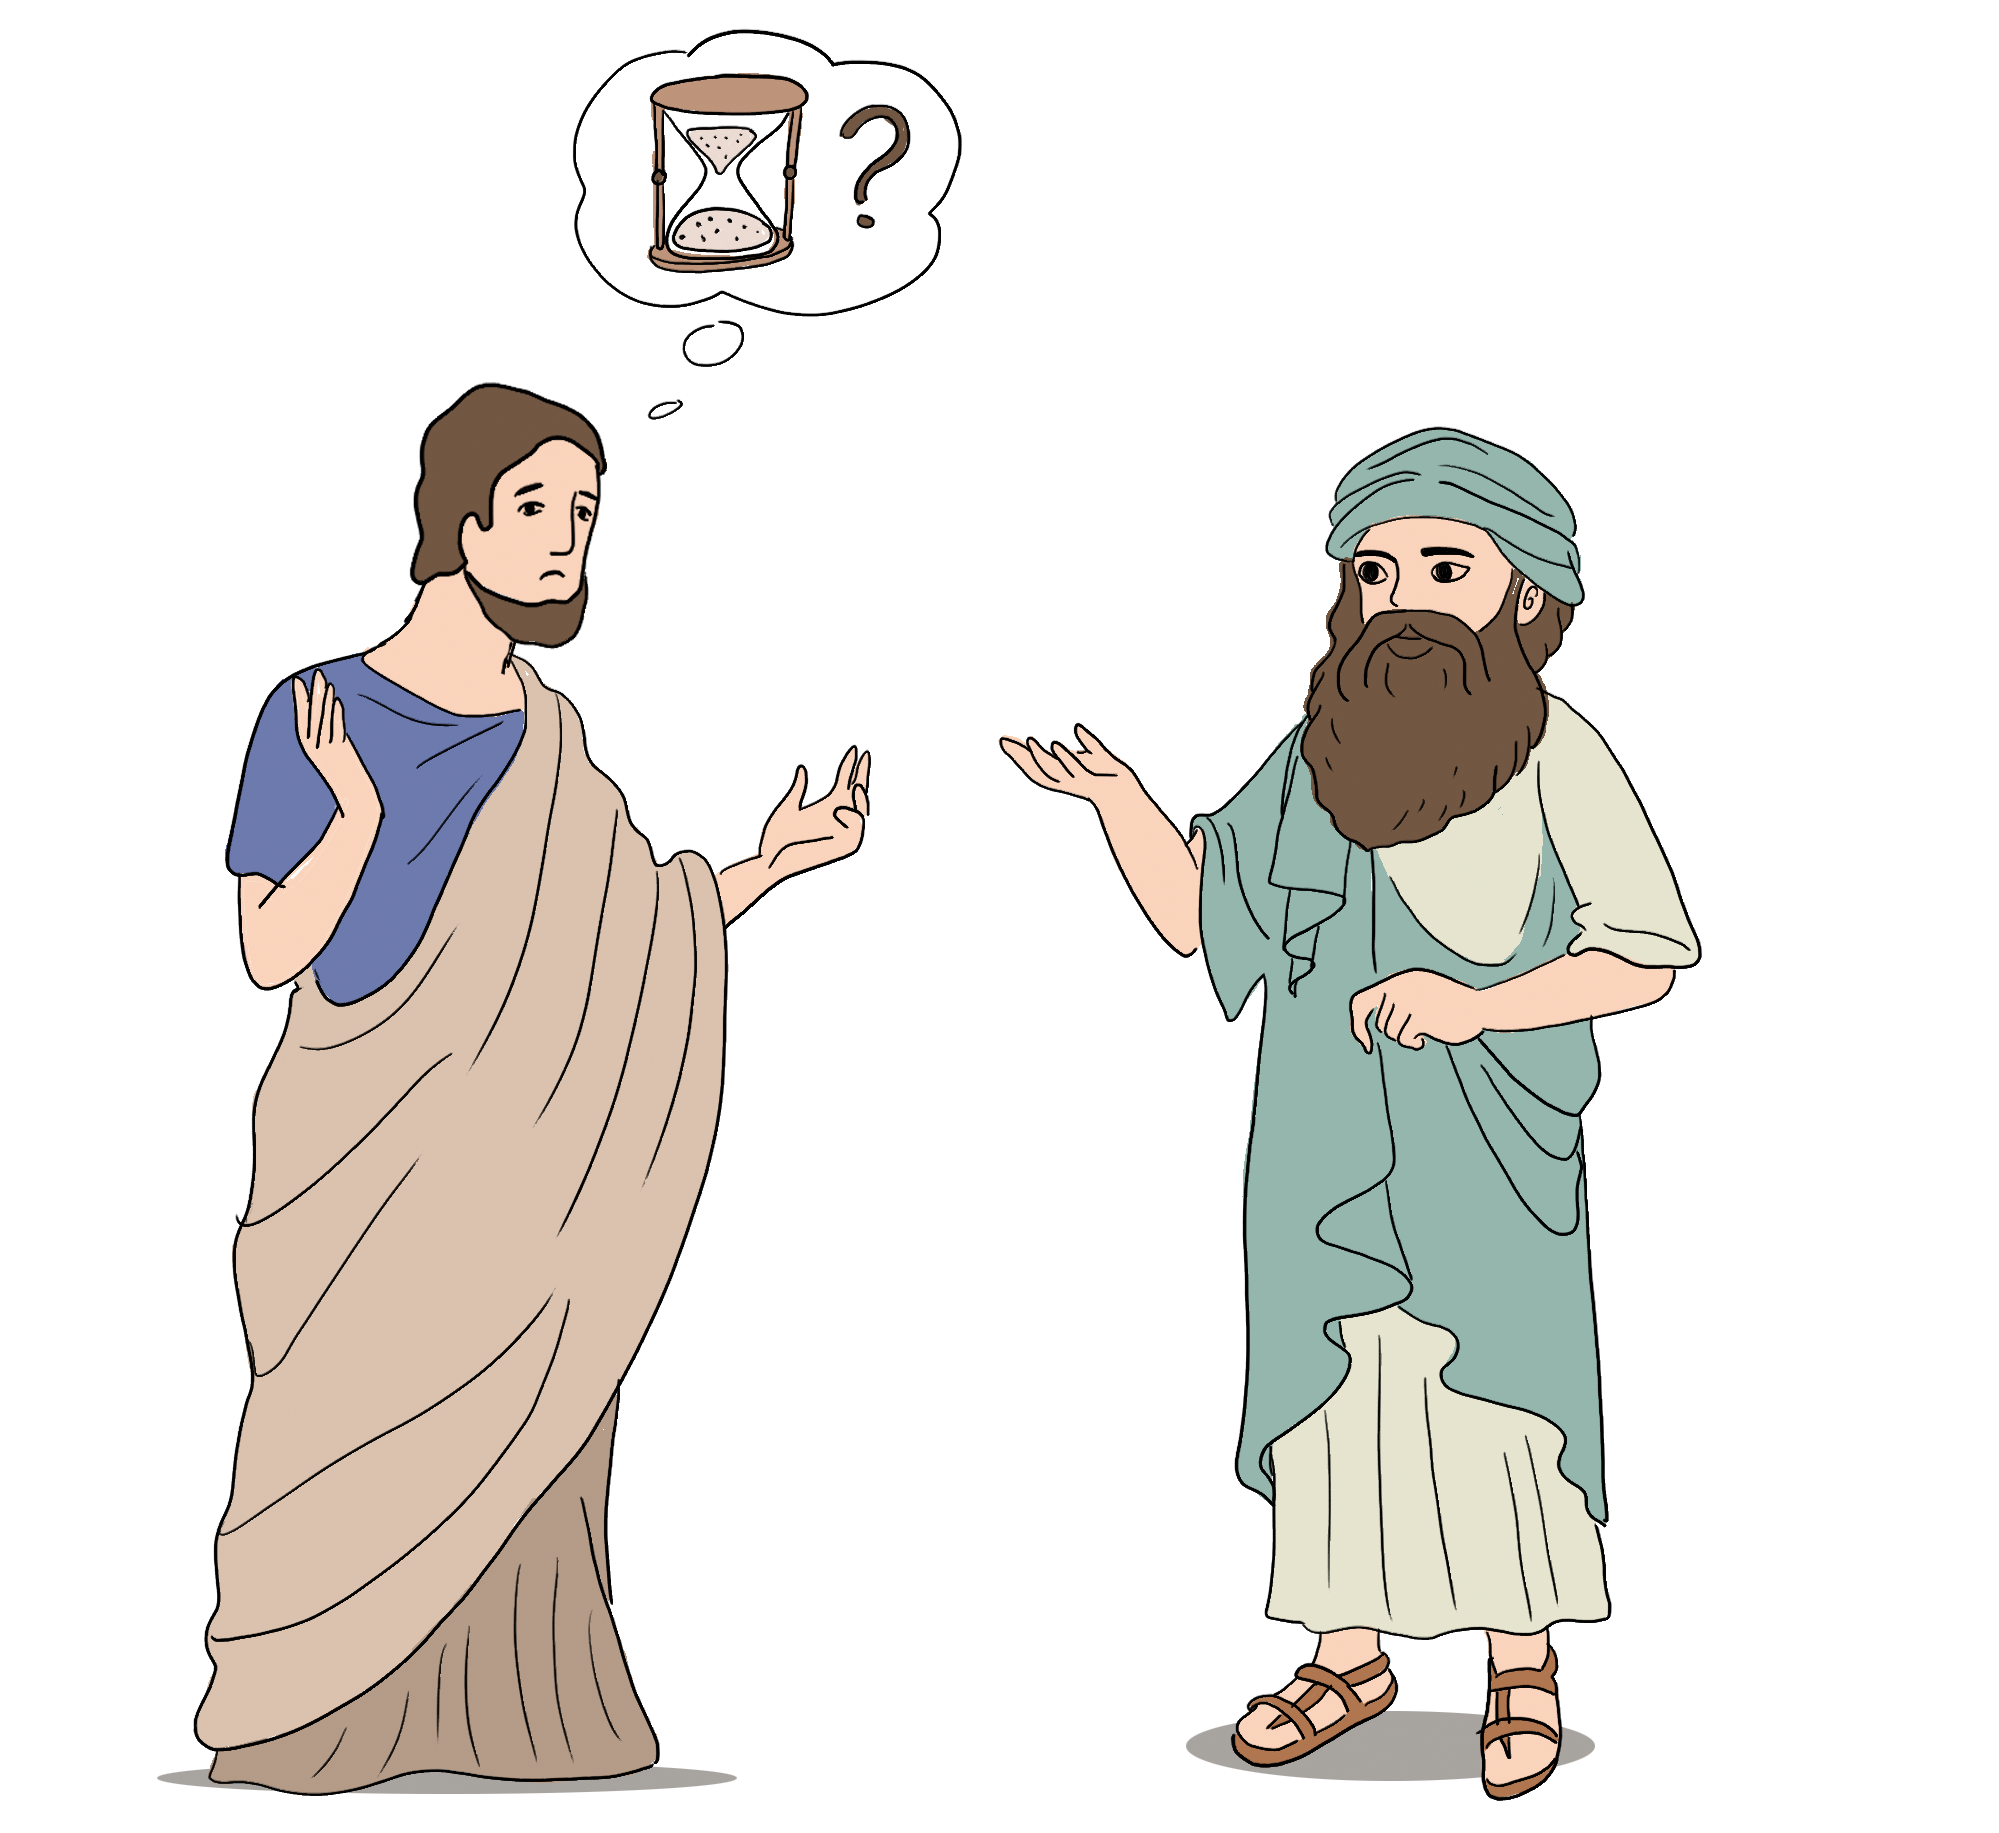
\includegraphics[width=0.7\linewidth]{Pi1_2_Bai2}
		\vspace*{-10pt}
	\end{figure}
	$\pmb{3.}$ Một tháng trước bà Hoa ra chợ mua một cân khoai tây, một cân thịt và một chục trứng. Chủ nhật vừa rồi, khoai tây tăng lên gấp $3$, thịt gấp $4$ lần còn trứng đắt gấp $5$ lần, nên bà Hoa phải trả $600$ nghìn cho từng ấy món hàng như lần thứ nhất. Hôm nay thì khoai lại đắt gấp $6$ lần so với tháng trước, thịt đắt gấp $5$ lần còn trứng chỉ đắt gấp $4$ lần nên bà Hoa lại phải trả $660$ nghìn với cùng một lượng hàng. Hỏi bà Hoa đã trả bao nhiêu tiền cho lần mua thứ nhất?
	\begin{figure}[H]
		\centering
		\vspace*{-10pt}
		\captionsetup{labelformat= empty, justification=centering}
		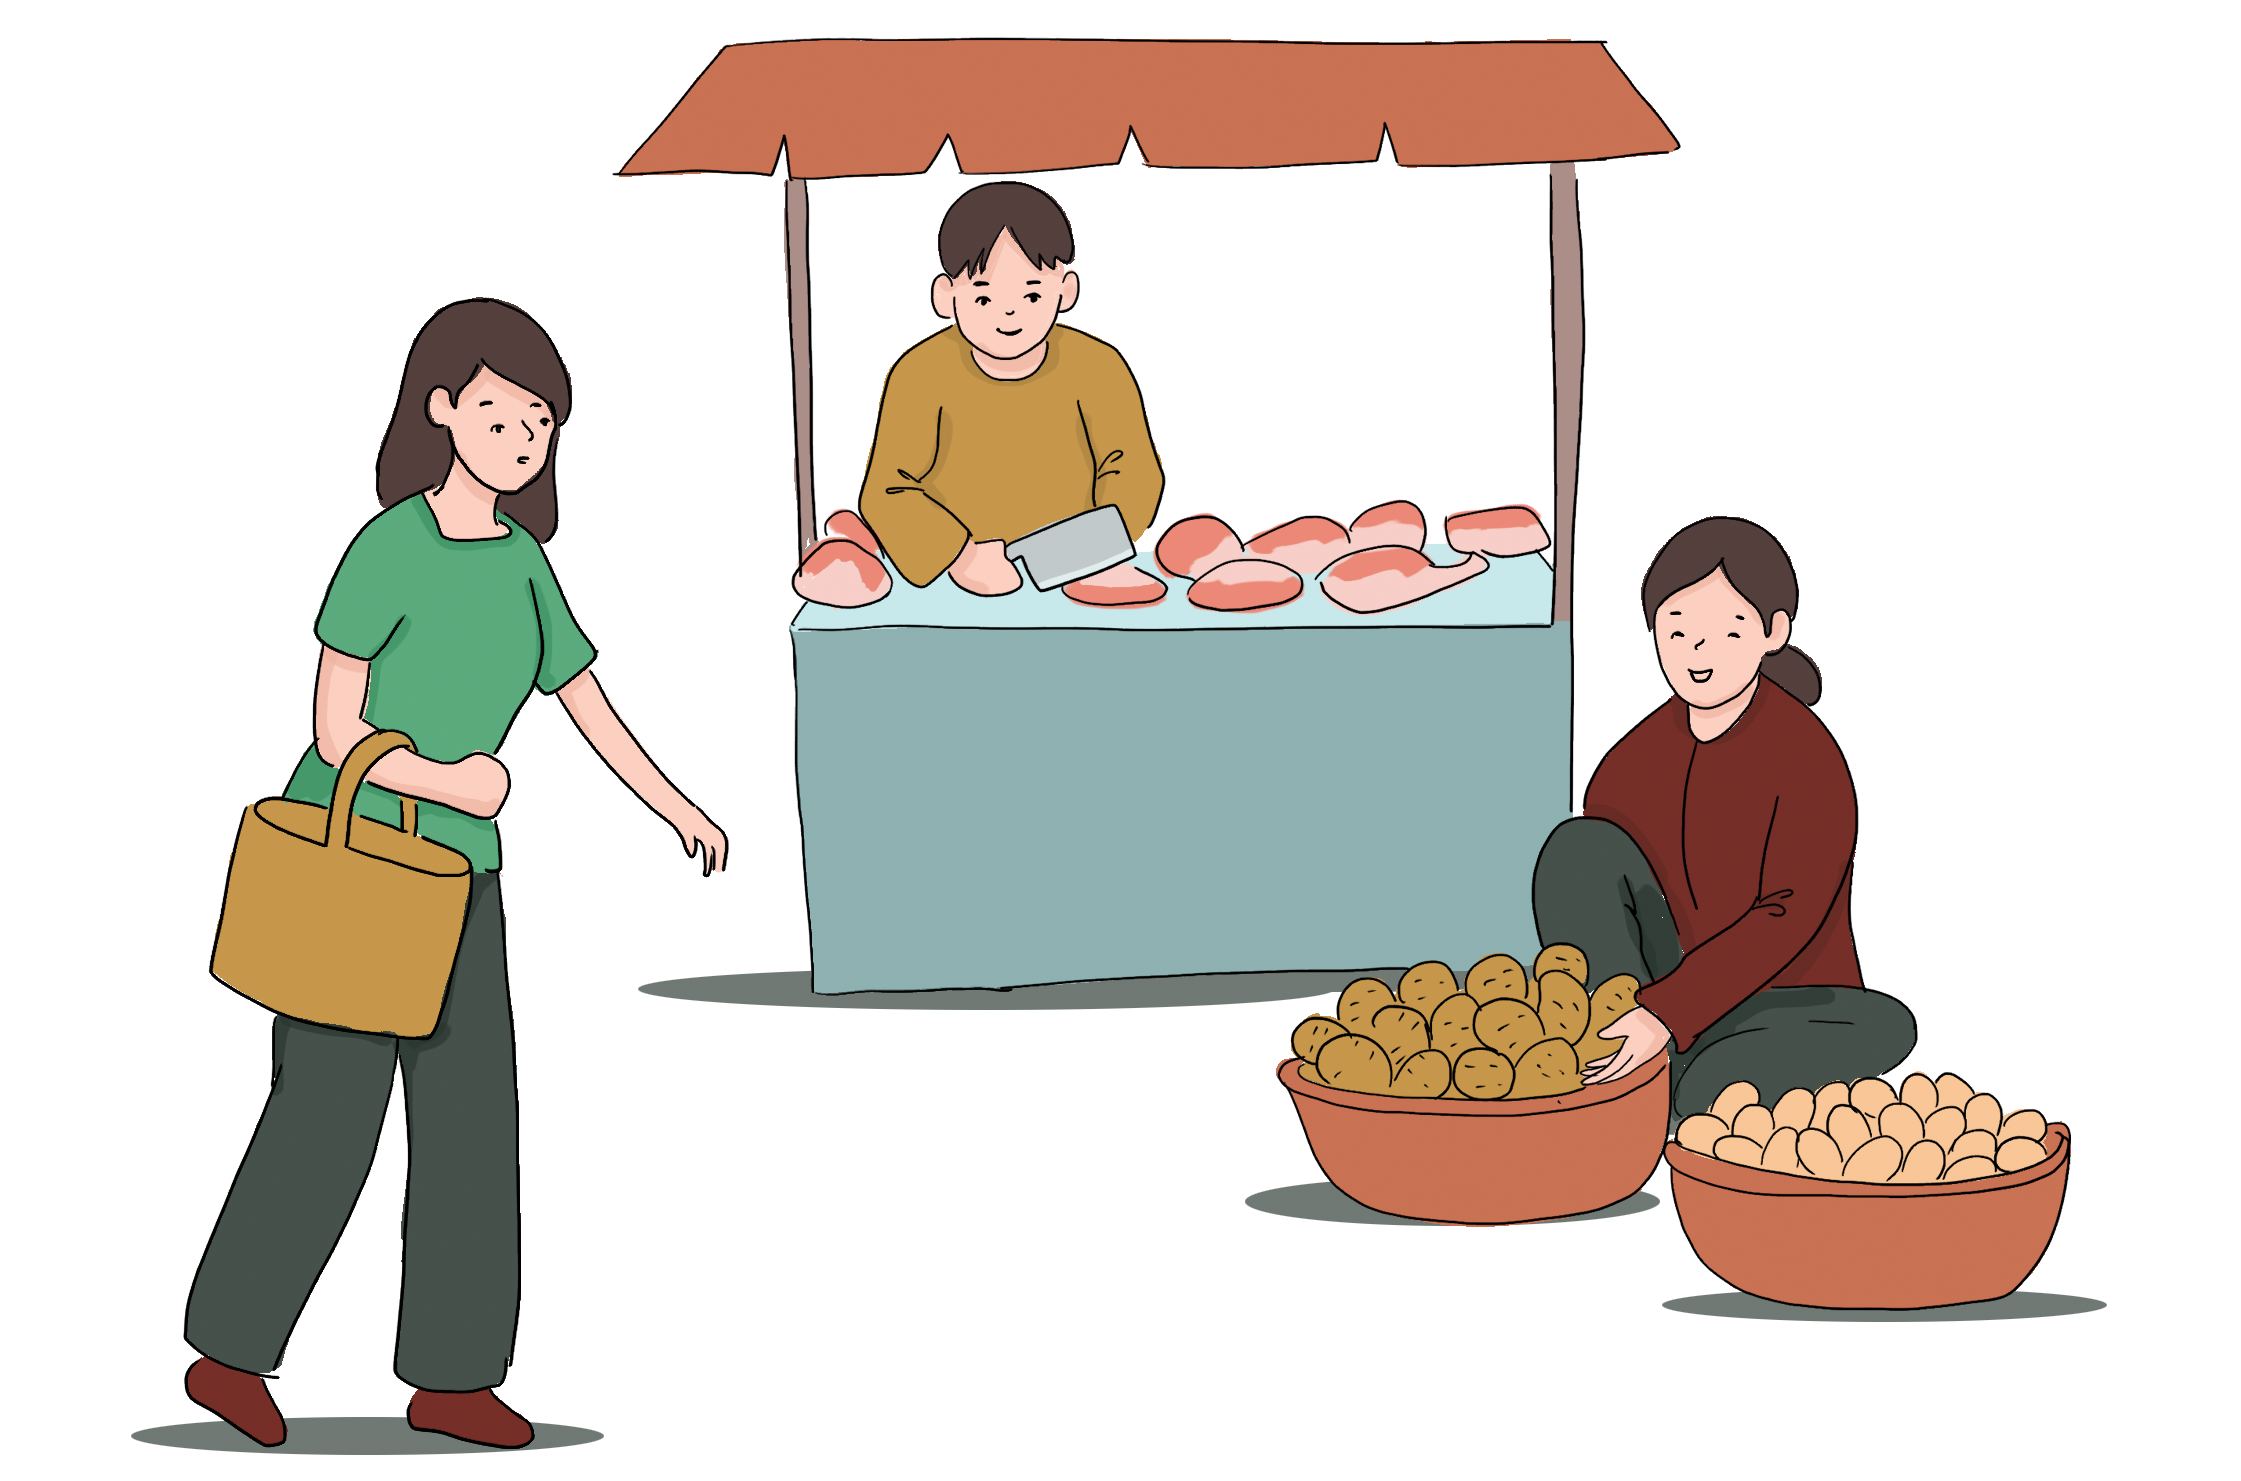
\includegraphics[width=0.9\linewidth]{Pi1_2_Bai3}
		\vspace*{-10pt}
	\end{figure}
	$\pmb{4.}$ Trong một buổi dạ hội nọ mỗi quý ông đã hân hạnh khiêu vũ với ba quý bà, còn mỗi quý bà cũng đã khiêu vũ với ba quý ông. Em hãy chỉ ra rằng số quý ông và số quý bà tham gia dạ hội là bằng nhau.
	\begin{figure}[H]
		\centering
		\vspace*{-5pt}
		\captionsetup{labelformat= empty, justification=centering}
		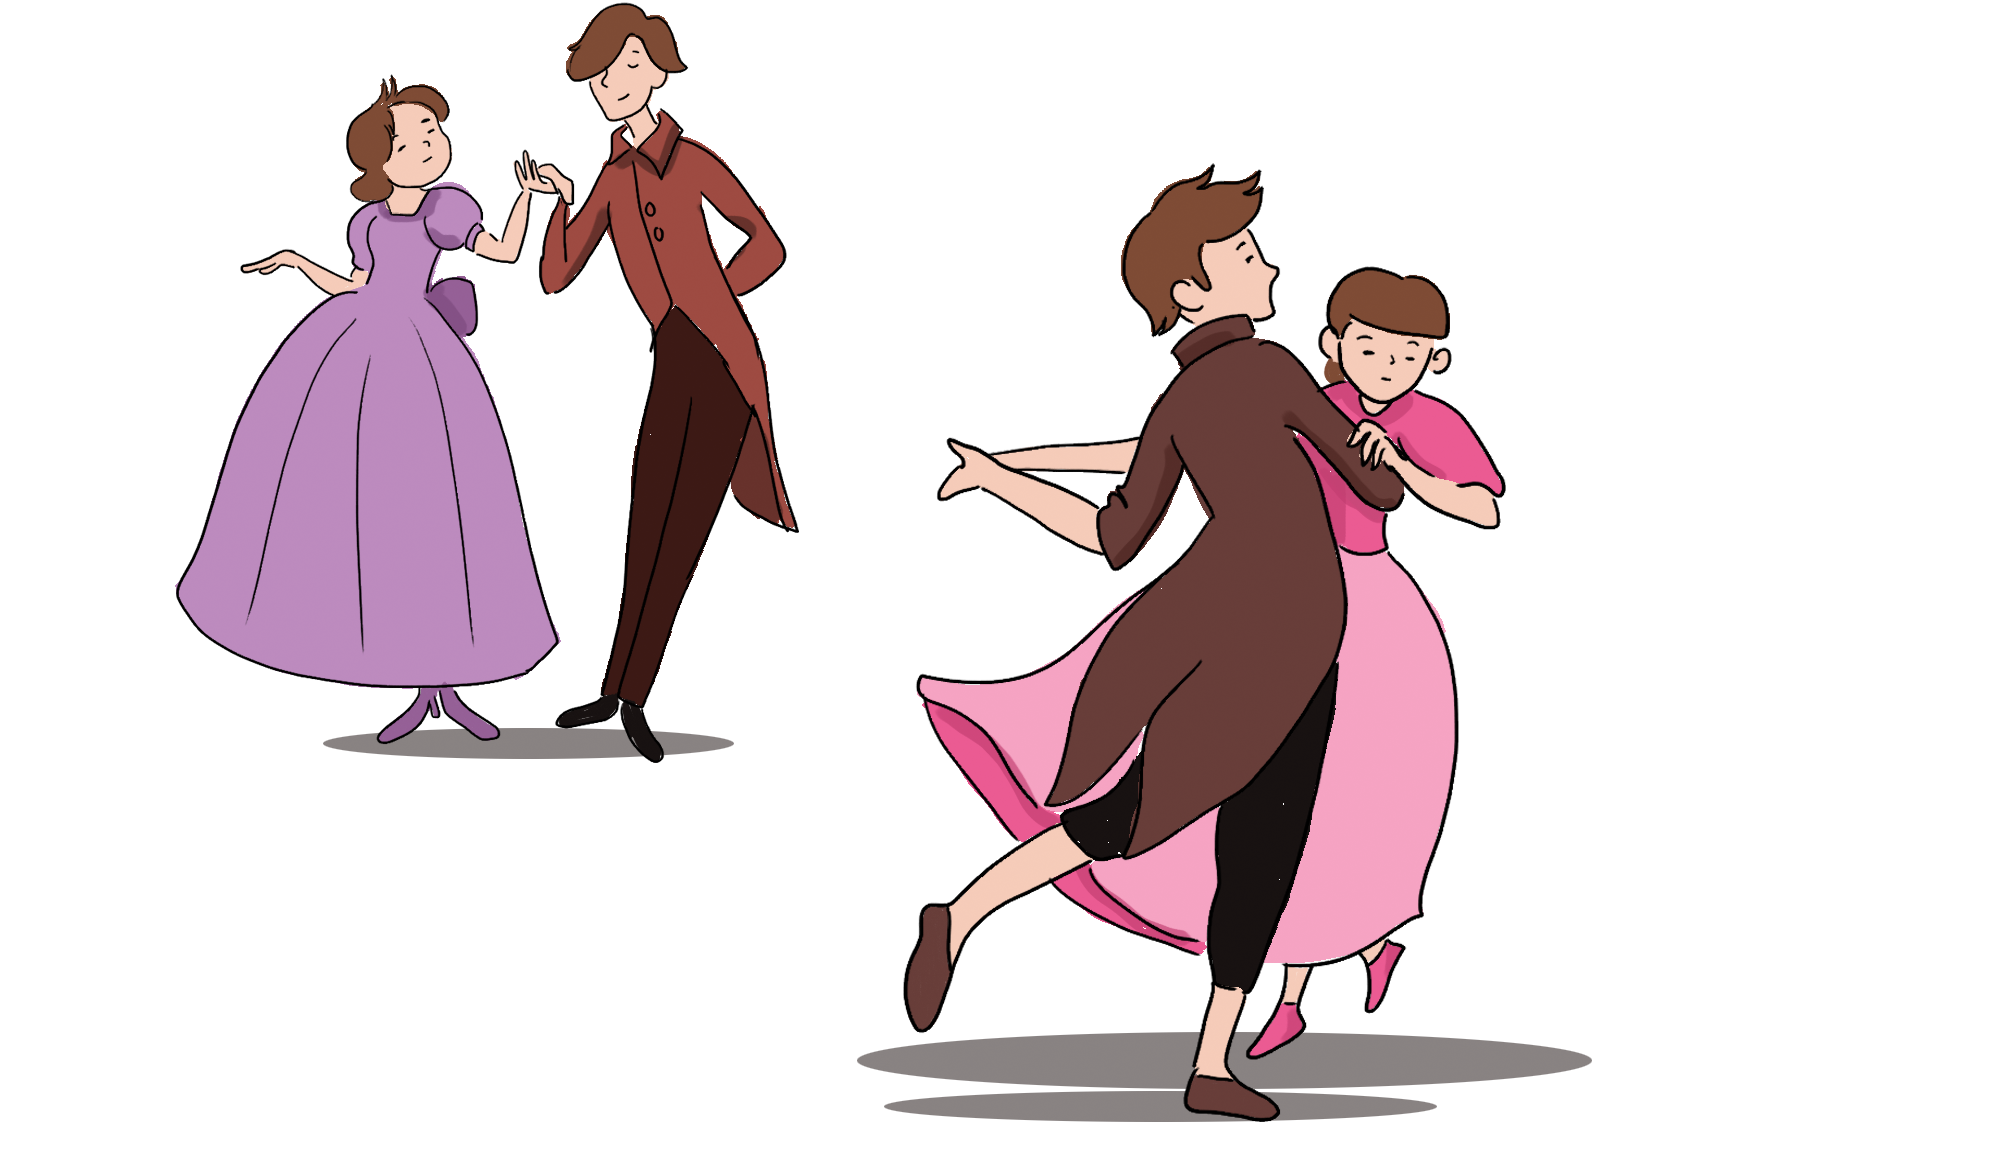
\includegraphics[width=1\linewidth]{Pi1_2_Bai4}
		\vspace*{-20pt}
	\end{figure}
	$\pmb{5.}$ 	Sau khi kết thúc một giải thi cờ vua, ban tổ chức nhận thấy mỗi kỳ thủ tham gia đã có số trận thắng khi chơi bằng quân trắng bằng đúng tổng số trận thắng của toàn bộ các kỳ thủ còn lại khi chơi quân đen. Em hãy chỉ ra rằng tất cả các kỳ thủ tham gia thi đấu đã có số trận thắng là như nhau.
	\begin{figure}[H]
		\centering
		\vspace*{-5pt}
		\captionsetup{labelformat= empty, justification=centering}
		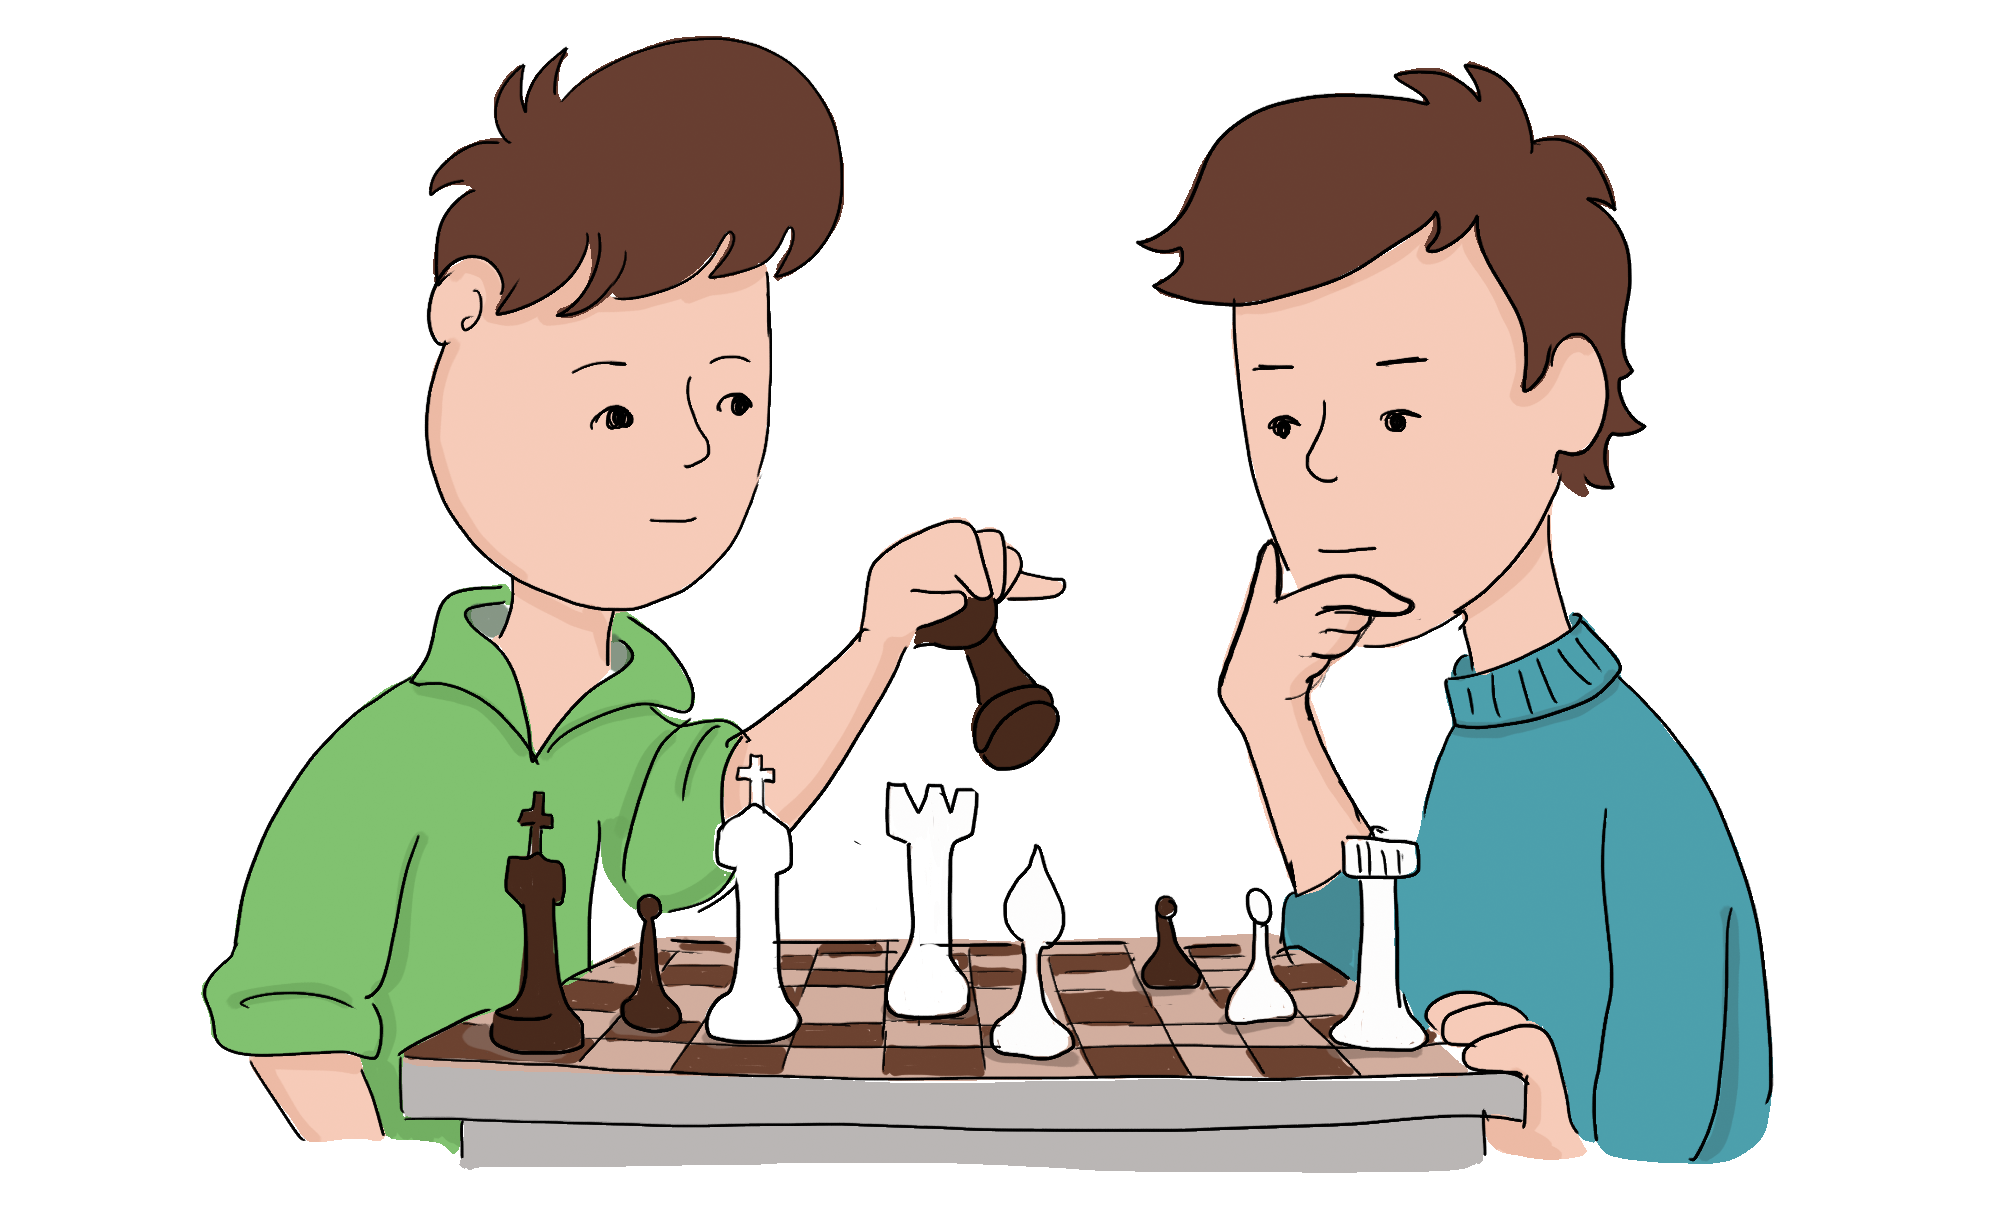
\includegraphics[width=0.75\linewidth]{Pi1_2_Bai5}
		\vspace*{-10pt}
	\end{figure}
	$\pmb{6.}$ Vào một ngày Chủ nhật nọ, Vinh và người em trai nhỏ tuổi hơn là Minh  đạp hai chiếc xe tới hiệu sách trung tâm cách nhà vài cây số. Tại đó mỗi người chọn mua một cuốn sách quý mà nhóm bạn bè cũ đang bàn luận khen ngợi thường xuyên mấy năm nay trên Facebook. Mỗi người đều lấy tổng tất cả các chữ số của tất cả các trang sách mình đã mua và nhận thấy rằng số đó bẳng năm sinh của mình. Vậy ai  trong số hai anh em Vinh và Minh  đang đi học lớp  bồi dưỡng Toán cho học sinh phổ thông nhỉ?
	\begin{figure}[H]
		\centering
		\vspace*{-5pt}
		\captionsetup{labelformat= empty, justification=centering}
		
\includegraphics[width=1\linewidth]{Pi1_2_Bai6}
		\vspace*{-10pt}
	\end{figure}
\end{multicols}
\newpage
\begingroup
\AddToShipoutPicture*{\put(112,643){
\includegraphics[scale=1]{../tieude2.pdf}}} 
\centering
\endgroup
\graphicspath{{../toancuabi/pic/}}
\vspace*{65pt}

\begin{multicols}{2}
	$\pmb{1.}$ Một chiếc tàu cao tốc dài $18$ m đi ngang qua một cột cây số trong vòng $9$ giây. Hỏi chiếc tàu đó cần bao nhiêu thời gian để đi qua hết một cây cầu dài $36$ m? 
	\begin{figure}[H]
		\centering
		\vspace*{-10pt}
		\captionsetup{labelformat= empty, justification=centering}
		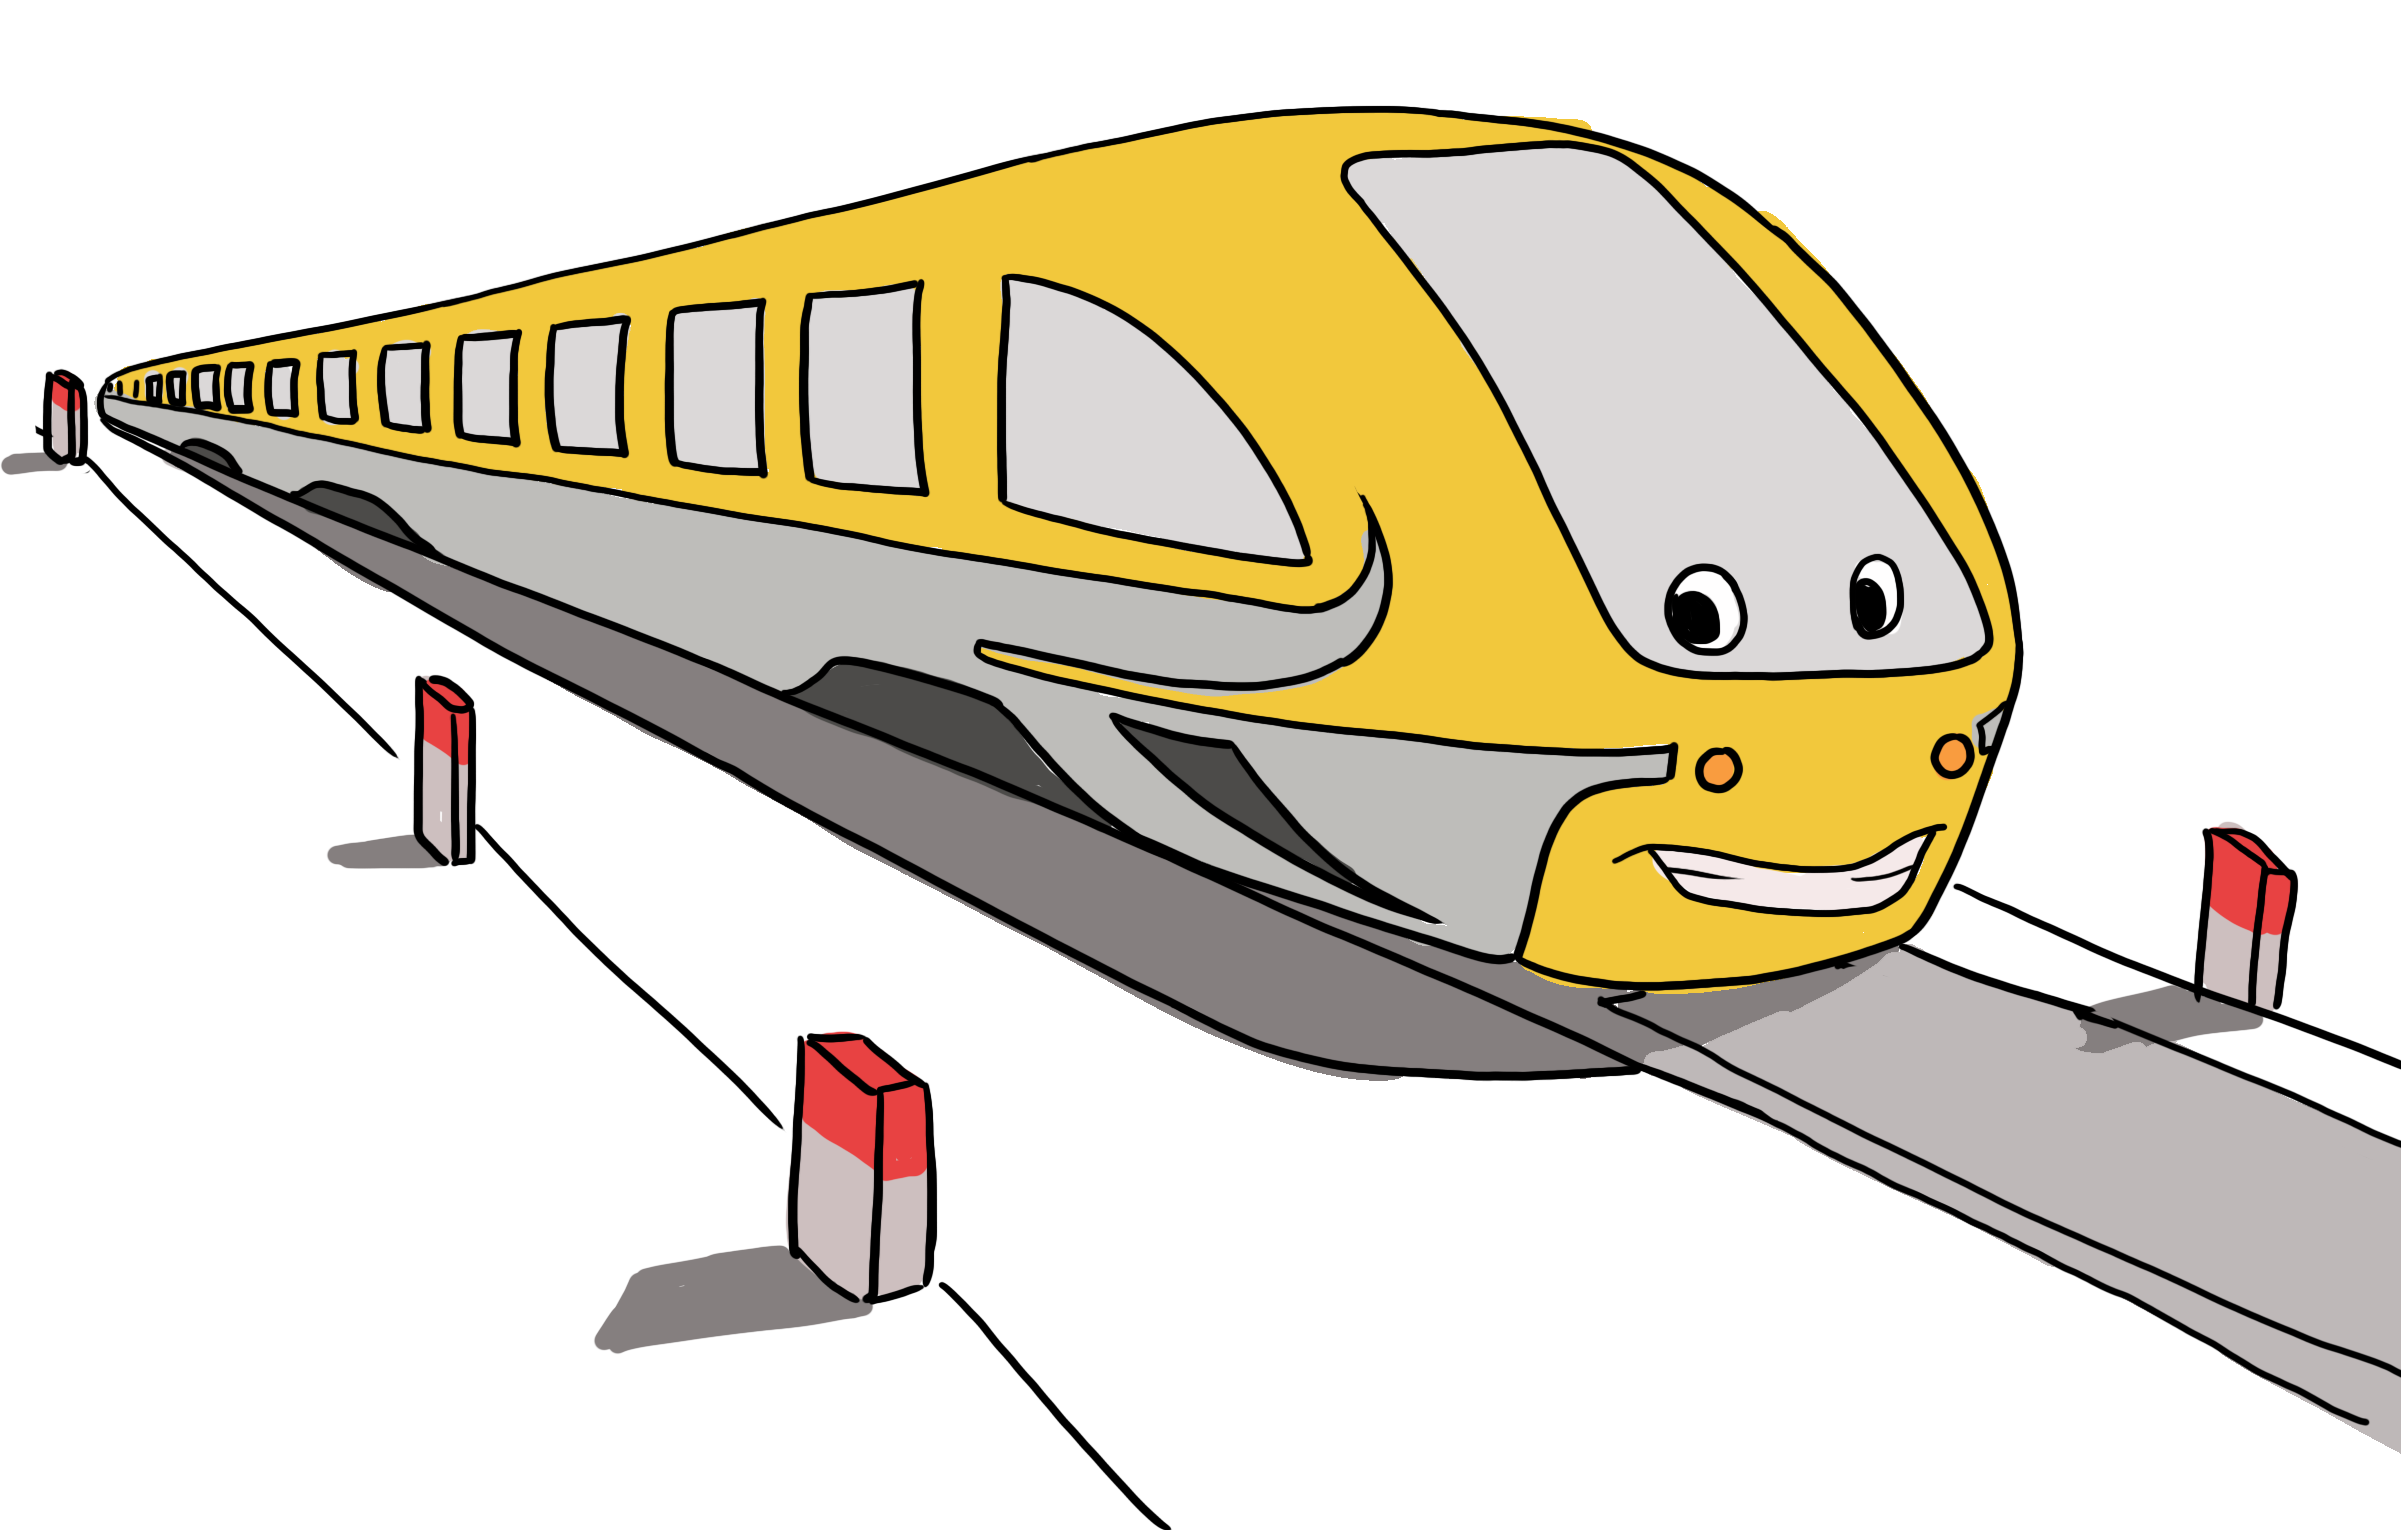
\includegraphics[width=1\linewidth]{Pi10_ToanBi_Bai1}
		\vspace*{-15pt}
	\end{figure}
	\textit{Lời giải.} 	Các em không cần phải tính vận tốc của chiếc tàu cao tốc mà vẫn có thể tìm ra đáp số đúng là $27$ giây. Thật vậy, thời gian tính từ khi đầu tàu đi tới cầu cho tới khi đuôi tàu đi hẳn vào cầu là $9$ giây. Sau $9$ giây đó, đầu tàu đi được đúng nửa cây cầu (do độ dài của tàu bằng nửa độ dài của cầu), và vì thế nó cần thêm $9$ giây để đi hết chiếc cầu. Đuôi tàu cũng cần thêm $9$ giây nữa để đi qua hết cầu. Vì thế tàu cao tốc cần tổng cộng $9+9+9= 27$ (giây) để đi qua hết cây cầu.
	\vskip 0.1cm
	$\pmb{2.}$ Hai cậu bé đi bán cam để gây quỹ xây dựng thư viện. Mỗi cậu có $30$ quả cam. Cậu thứ nhất bán  $10{.}000$ đồng/$2$ quả cam, cậu thứ hai bán $10{.}000$ đồng/$3$ quả cam. Trong lúc đang chuẩn bị bày cam ra bán thì một cậu bị gọi về nhà nên cậu ta nhờ cậu thứ hai bán hộ số cam của mình. Tất cả số cam còn lại được cậu bé thứ hai bán với giá $20{.}000$ đồng/$5$ quả cam. Nếu như số cam bán riêng như dự định lúc đầu thì đã thu được là $150{.}000$ đồng và $100{.}000$ đồng, tức là tổng cộng có $250{.}000$ đồng, nhưng vì bán gộp $20{.}000$ đồng cho $5$ quả nên  hai cậu chỉ thu được $240{.}000$ đồng. Hỏi số tiền bị hụt $10{.}000$ đồng đã mất ở chỗ nào?
	\vskip 0.1cm
	\textit{Lời giải.} Tổng số cam của hai bạn là  $30 + 30=60$ (quả). Ta xếp chúng thành $2$ loại:
	\vskip 0.1cm
	-- Loại $1$: gồm $10$ phần, mỗi phần gồm $5$ quả;
	\vskip 0.1cm
	-- Loại $2$: $10$ quả còn lại.
	\vskip 0.1cm
	Trong mỗi phần ở Loại $1$, ta bán $2$ quả theo giá của bạn thứ nhất và $3$ quả theo giá của bạn thứ $2$. Như vậy, bán mỗi phần này  thu được $20{.}000$ nghìn và theo cách bán này thì mỗi phần thu được số tiền đúng như cách bán của cả hai kiểu.
	\begin{figure}[H]
		\centering
		\vspace*{-10pt}
		\captionsetup{labelformat= empty, justification=centering}
		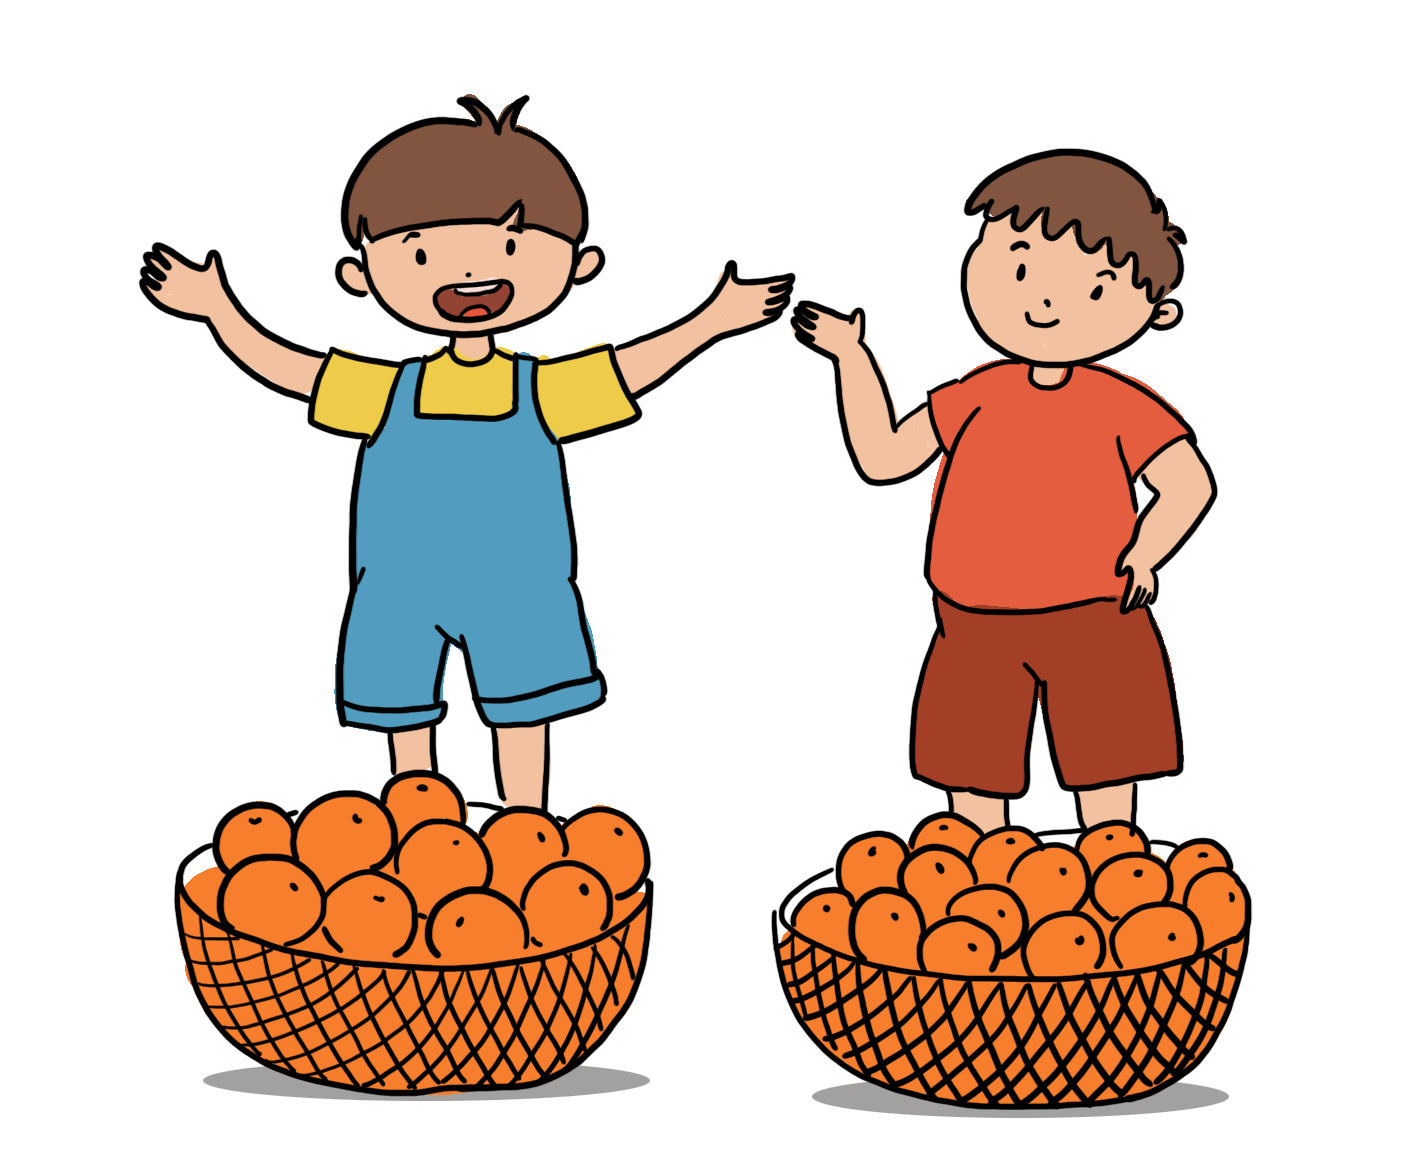
\includegraphics[width=0.9\linewidth]{Pi10_ToanBi_Bai2}
		\vspace*{-10pt}
	\end{figure}
	-- Nếu bán như ban đầu, $10$ quả còn lại sẽ bán theo giá của bạn thứ nhất ($10{.}000$ đồng/$2$ quả)
	\vskip 0.1cm
	-- Nếu bán theo cách sau, trong $10$ quả còn lại chỉ có $4$ quả cam được theo giá ban đầu ($10{.}000$ đồng/$2$ quả) và $6$ quả bị bán với giá rẻ hơn ($10{.}000$ đồng/$3$ quả).
	\vskip 0.1cm
	Từ đó theo cách bán sau, số tiền bị thiệt đi là:
	\setlength{\abovedisplayskip}{5pt}
	\setlength{\belowdisplayskip}{5pt}
	\begin{align*}
		6\times\frac{10{.}000}{2} - 6\times\frac{10{.}000}{3} = 10{.}000.
	\end{align*}
	\textit{Cách giải khác.}
	\vskip 0.1cm
	Theo cách bán ban đầu: mỗi quả cam của bạn thứ nhất có giá là: $\dfrac{10{.}000}{2}$ đồng, mỗi quả cam của bạn thứ hai có giá là: $\dfrac{10{.}000}{3}$ đồng.
	\vskip 0.1cm
	Theo cách bán sau thì giá của mỗi quả cam là $\dfrac{20{.}000}{5}$ đồng.
	\vskip 0.1cm
	Như vậy, cứ $2$ quả cam thì bán theo cách sau bị thiệt:
	\begin{align*}
		\dfrac{10{.}000}{2} + \dfrac{10{.}000}{3} - 2\times\dfrac{20{.}000}{5} = \dfrac{1{.}000}{3}.
	\end{align*}
	Vậy khi bán $60$ quả cam thì theo cách sau, cậu bé thứ hai bị mất đi số tiền là:
	\begin{align*}
		30\times \dfrac{1{.}000}{3} = 10{.}000 \text{ (đồng)}
	\end{align*}
	$\pmb{3.}$ Có ba người bạn tập trung lại để đi cắm trại và họ chỉ có duy nhất một chiếc xe máy có $2$ chỗ ngồi. Liệu họ có thể vượt được quãng đường dài $60$ km tới nơi cắm trại sau khoảng thời gian $3$ giờ đồng hồ được hay không, biết rằng vận tốc của mỗi người đi bộ là $5$ km/giờ và vận tốc của xe máy (có tải hay không có tải) luôn là $50$ km/giờ?
	\begin{figure}[H]
		\centering
		\vspace*{-15pt}
		\captionsetup{labelformat= empty, justification=centering}
		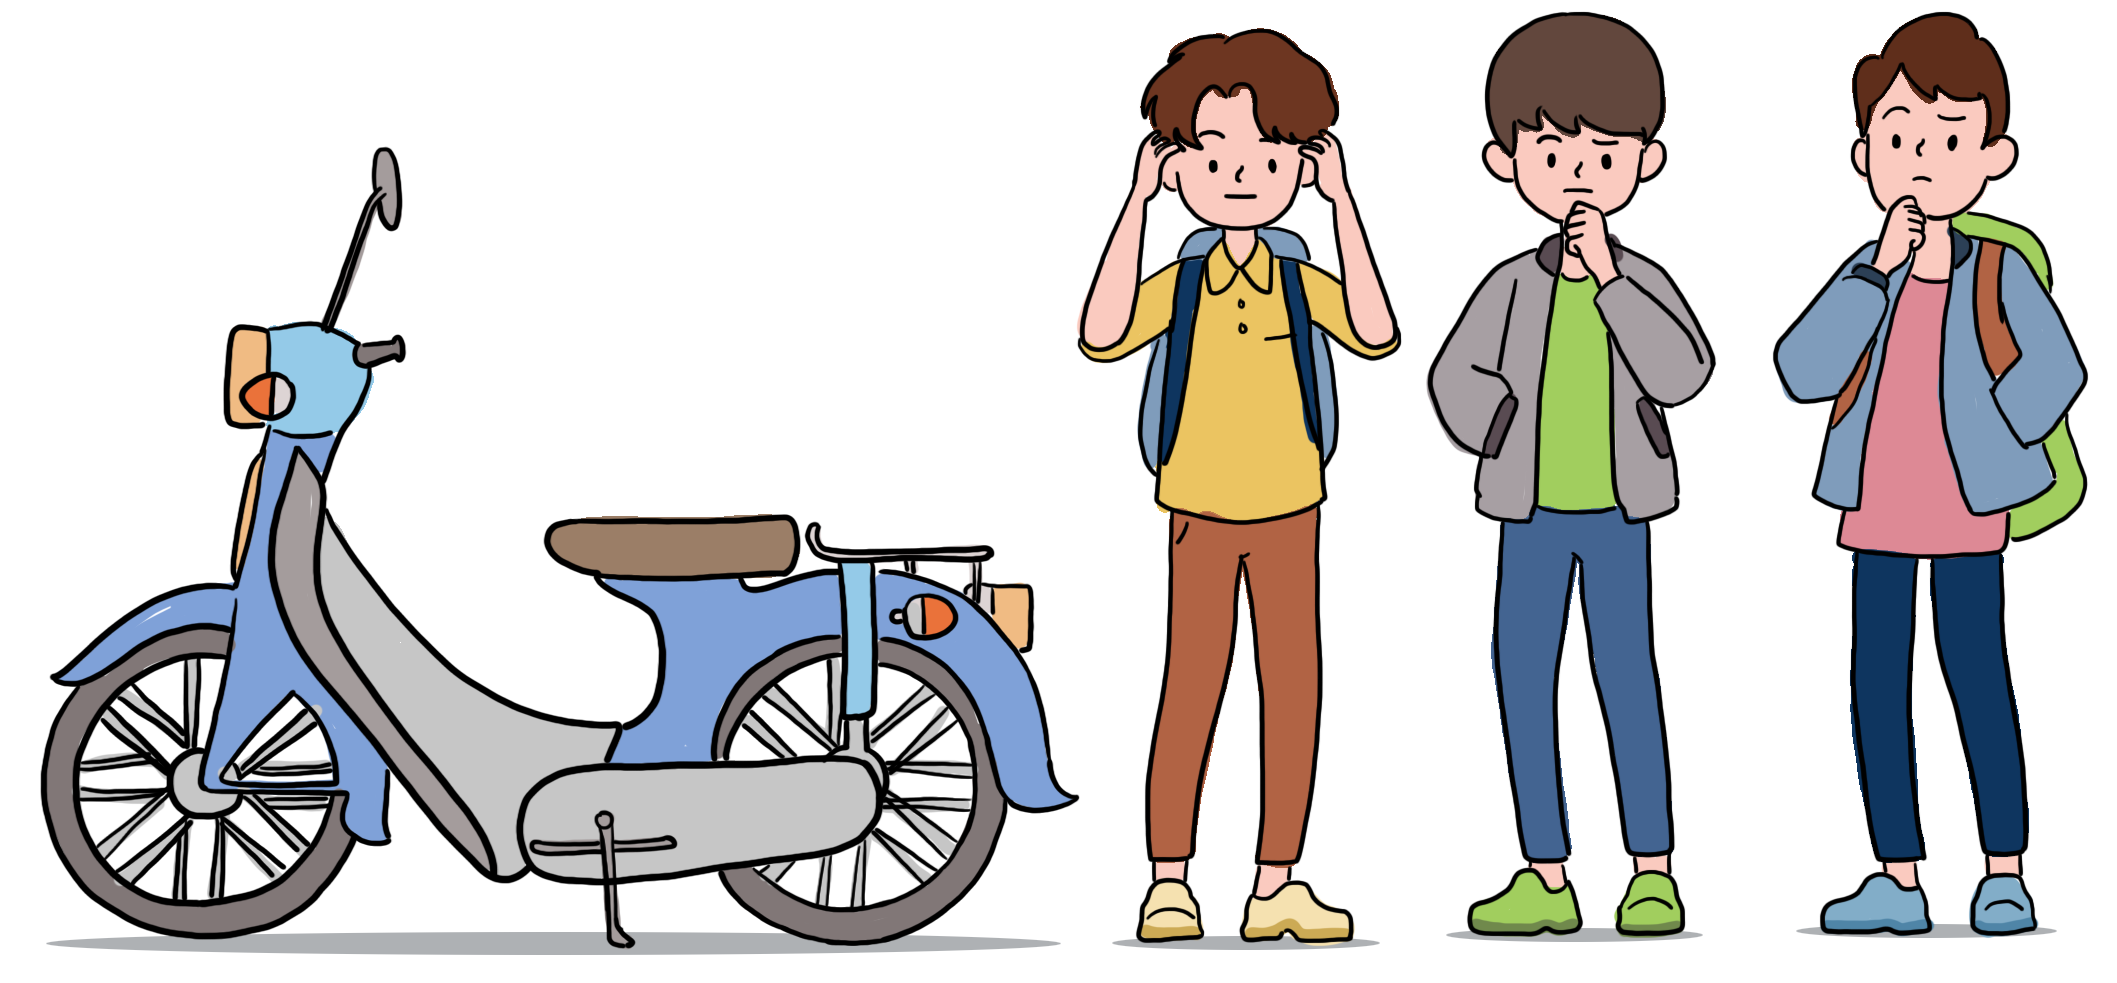
\includegraphics[width=1\linewidth]{Pi10_ToanBi_Bai3}
		\vspace*{-15pt}
	\end{figure}
	\textit{Lời giải.} 	Ta gọi $3$ người đó là $A$, $B$, $C$. Trước tiên $A$ sẽ chở $B$ đi bằng xe máy và để $C$ tự đi bộ. Sau $1$ giờ, hai người đi bằng xe máy đi được quãng đường là $50$ km. Khi này, $A$ để $B$ xuống, cho $B$ đi bộ đến nơi cắm trại còn $A$ quay ngược trở lại để đón $C$. Để đi quãng đường còn lại tới nơi cắm trại là $60-50=10$ km, anh $B$ cần đi bộ thêm trong vòng $10 : 5= 2$ (giờ). Khi $A$ bắt đầu quay trở lại, anh $C$ đã đi bộ được quãng đường là $5$ km. Nghĩa là, khi này, $A$ và $C$ cách nhau quãng đường là $50-5=45$ (km). Mỗi giờ quãng đường mà cả hai đi được là $50+5=55$ (km). Do $A$ và $C$ di chuyển ngược chiều nhau, thời gian để họ bắt gặp nhau là: $45: 55= \dfrac{9}{11} $ (giờ). Khi $A$ và $C$ gặp nhau, $C$ đã đi thêm được $5\times \dfrac{9}{11}= \dfrac{45}{11}$. Như vậy, lúc này tổng quãng đường mà $C$ đã đi được là
	$5 + \dfrac{45}{11}= \dfrac{100}{11}$ (km). Do đó, khi $A$ và $C$ gặp nhau thì họ cách điểm cắm trại một quãng đường là $60- \dfrac{100}{11}= \dfrac{560}{11}$ (km). Vì vậy, $A$ có thể chở $C$ đến nơi cắm trại trong khoảng thời gian là $\dfrac{560}{11}: 50= \dfrac{56}{55}$ (giờ).
	\vskip 0.1cm
	Như vậy, khi $C$ và $A$ đến nơi cắm trại thì thời gian mà $C$ đã đi là $1 + \dfrac{9}{11}+ \dfrac{56}{55}=1 + \dfrac{101}{55}= 2\dfrac{46}{55}$ (giờ). Nghĩa là $C$ và $A$ cũng đến được điểm cắm trại sau $3$ giờ. Vì vậy, với cách đi như trên, sau $3$ giờ thì cả ba người đều đến được nơi cắm trại.
	\vskip 0.1cm
	$\pmb{4.}$ Có $100$ chiếc thẻ bài bằng nhựa đánh số từ $1$ tới $100$ lần lượt được xếp thành hàng ngang. Cứ hai chiếc thẻ xếp cách nhau một chiếc thẻ khác đều có thể đổi chỗ được cho nhau. Liệu em có thể đổi chỗ các chiếc thẻ này bằng cách như trên để xếp lại được $100$ chiếc thẻ trên theo thứ tự ngược lại được hay không?
	\begin{figure}[H]
		\centering
		\vspace*{-10pt}
		\captionsetup{labelformat= empty, justification=centering}
		\includegraphics[width=0.98\linewidth]{Pi10_ToanBi_Bai4}
		\vspace*{-10pt}
	\end{figure}
	\textit{Lời giải.} 	Mỗi lần đổi chỗ, một chiếc thẻ sẽ di chuyển vị trí là $+2$ hoặc $-2$ so với vị trí cũ. Như vậy theo cách đổi chỗ như trên, một chiếc thẻ sẽ luôn thay đổi một số chẵn vị trí. Nếu có thể sắp xếp các chiếc thẻ theo thứ tự ngược lại thì chiếc thẻ mang số $1$, ban đầu ở vị trí số $1$, cần phải được chuyển đến vị trí số $100$, nghĩa là cần thay đổi $99$ vị trí so với ban đầu. Đây là một số lẻ. Suy ra ta không thể xếp lại $100$ chiếc thẻ theo thứ tự ngược lại.
	\vskip 0.1cm
	$\pmb{5.}$ Trong ngày khai giảng các bạn học sinh gặp lại nhau sau một mùa hè nên vô cùng mừng rỡ. Gặp lại bạn bè cũ và ai cũng tranh thủ bắt tay bạn mình. Kết thúc màn chào hỏi vui tươi sôi nổi, anh phụ trách thống kê lại trong cuốn sổ các bạn học sinh đã có số lẻ lần bắt tay và tổng cộng có $67$ bạn. Bạn Lâm đứng cạnh anh phụ trách nói nhỏ ``Anh ơi, anh đếm nhầm rồi, chắc chắn không phải là $67$ bạn ạ". Anh phụ trách vô cùng ngạc nhiên, vì sao Lâm lại biết vậy. Em có thể giải thích vì sao Lâm lại cho rằng anh phụ trách đếm nhầm được không?
	\begin{figure}[H]
		\centering
		\vspace*{-10pt}
		\captionsetup{labelformat= empty, justification=centering}
		\includegraphics[width=1\linewidth]{Pi10_ToanBi_Bai5}
		\vspace*{-15pt}
	\end{figure}
	\textit{Lời giải.} 	Khi một bạn $A$ bắt tay một bạn $B$ của mình, thì $B$ cũng bắt tay $A$, vì thế nếu $P$ là tổng số lượt bắt tay của tất cả các bạn học sinh thì $P= 2+2+\cdots+2=2n$ phải là một số chẵn.
	\vskip 0.1cm
	Ta chia $P$ thành hai tổng. Tổng thứ nhất, ký là $Q$, là số lượt bắt tay của các bạn thực hiện một số chẵn lần bắt tay. Tổng thứ hai, ký hiệu là $R$, là số lượt bắt tay của các bạn thực hiện một số lẻ lần bắt tay. Rõ ràng $P= Q+R$, và $Q$ phải là số chẵn. Vì thế $R = P - Q$ cũng phải là số chẵn. Vì vậy số các bạn có số lẻ lần bắt tay không thể bằng $67$, vì nếu như vậy $R$ sẽ là số lẻ (là tổng của $67$ số lẻ). Do đó Lâm biết được anh phụ trách đã đếm nhầm. Các em cũng có thể thấy từ bài này rằng số các bạn có số lẻ lần bắt tay phải luôn là số chẵn, thú vị phải không nào?
	\vskip 0.1cm
	$\pmb{6.}$ $a)$  Có $50$ vị khách ngồi xung quanh một chiếc bàn tròn được xếp đều, trong số họ có $25$ phụ nữ. Em hãy chứng tỏ rằng có một vị khách ngồi cạnh hai phụ nữ.
	\vskip 0.1cm
	$b)$ Giả sử bây giờ số phụ nữ là $26$ người. Trong buổi tiệc bỗng dưng có hai vị khách làm vỡ mất hai chiếc cốc đặt trước mặt họ. Em hãy chứng tỏ rằng có thể xoay lại chiếc bàn tròn theo một cách nào đó để sao cho hai chiếc cốc vỡ lại đặt trước mặt của hai vị khách~nữ.
	\begin{figure}[H]
		\centering
		\vspace*{-10pt}
		\captionsetup{labelformat= empty, justification=centering}
		\includegraphics[width=1\linewidth]{Pi10_ToanBi_Bai6}
		\vspace*{-15pt}
	\end{figure}
	\textit{Lời giải.} $a)$ Để tiện hình dung, ta coi các vị khách ngồi ở các đỉnh của một hình đa giác $50$ cạnh đều. Ta chia hình đa giác $50$ cạnh thành hai hình $25$--giác đều (với các đỉnh xếp đan xen nhau). Do số phụ nữ là $25$ nên theo nguyên lý Dirichlet phải có một trong các hình $25$--giác đều này có ít nhất $13$ phụ nữ ngồi ở các đỉnh của nó. Nhưng do $13>\dfrac{25}{2}$ nên cũng theo nguyên lý Dirichlet, phải có hai phụ nữ ngồi ở hai đỉnh liên tiếp của $25$--giác đều này, vì thế ở giữa họ chỉ có một đỉnh duy nhất của hình $50$--giác ban đầu -- đó chính là vị trí của vị khách cần tìm.
	\vskip 0.1cm
	$b)$ Giả sử hai vị khách làm vỡ cốc ngồi ở hai đỉnh được nối với nhau bởi một đường chéo có độ dài là $a$. Ta sẽ phải tìm hai vị khách nữ cũng ngồi cách nhau một khoảng bằng $a$.
	\vskip 0.1cm
	Nếu $a$ không phải là độ dài của đường chéo dài nhất, thì từ mỗi một vị khách nữ có tất cả hai đường chéo xuất phát từ đó có độ dài $a$. Có tất cả $26\times 2= 52$ đường chéo như vậy. Tuy nhiên số đường chéo có độ dài $a$ chỉ là $50$, vì thế phải có hai đường chéo trong số $52$ đường trên trùng nhau. Ta giả sử đó là đường chéo $AB$. Khi đó $AB=a$, và có hai phụ nữ ngồi tại vị trí $A$ và $B$ là hai vị khách nữ cần tìm.
\end{multicols}
\newpage
\begingroup
\thispagestyle{toancuabinone}
\blfootnote{$^1$\color{toancuabi}Ottawa, Canada.}
\AddToShipoutPicture*{\put(60,733){\includegraphics[width=17.2cm]{../mathc.pdf}}}
%\AddToShipoutPicture*{\put(-2,733){\includegraphics[width=17.2cm]{../mathl.pdf}}} 
\AddToShipoutPicture*{\put(189,675){\includegraphics[scale=1]{../tieude4.pdf}}} 
\centering
\endgroup
\graphicspath{{../toancuabi/pic/}}
\vspace*{30pt}

\begin{multicols}{2}
	The diagram below is an example of a \emph{family tree}. The circles denote females and the triangles denote males.
	\begin{figure}[H]
		\vspace*{-5pt}
		\centering
		\captionsetup{labelformat= empty, justification=centering}
		\includegraphics[width= 0.75\linewidth]{hc-2022-2-3-15-1.pdf}
		\vspace*{-10pt}
	\end{figure}
	$A$ and $B$ are married, as are $F$ and $G,$ and $J$ and $K.$
	\vskip 0.1cm
	$B, C,$ and $D$ are siblings, as are $E$ and $F.$
	$E$ and $F$ are children of $A$ and $B.$
	\vskip 0.1cm
	Similarly, the parents of $I$ and $J$ are $F$ and $G.$
	$E$ is the father of $H.$
	\vskip 0.1cm
	In addition, $A$ is the grandmother of $H, I,$ and $J,$
	$F$ is the aunt of $H,$ and $C$ is the sister--in--law of $A.$
	\begin{figure}[H]
		\vspace*{-5pt}
		\centering
		\captionsetup{labelformat= empty, justification=centering}
		\includegraphics[width= 0.92\linewidth]{tree1}
		%		\vspace*{-5pt}
	\end{figure}
	
	\vspace*{0.1pt}
	
	\vspace*{-7pt}
	\PIbox{
		{\color{toancuabi}\textbf{Example} (Who is who)\textbf{.}}
		Inspector Jade asked six children to briefly introduce their brothers, sisters,
		and first cousins (cousins who share a grandparent). She had to match the name of each child to a numbered position in the family tree with the responses given below. Note that the relations were given in the local language. \emph{Please do not try to guess the genders of the children from the names. It may lead you to wrong conclusions.}
		\vskip 0.1cm
		Response from Binh:
		\vskip 0.1cm
		$\circ$ I have three \textit{arawa}: Kim, Minh, Thao
		\vskip 0.1cm
		$\circ$ I have two \textit{surubu}: Oanh and Yen
		\vskip 0.1cm
		Response from Dinh:
		\vskip 0.1cm
		$\circ$ I have two \textit{surubu}: Oanh and Yen
		\vskip 0.1cm
		$\circ$ I have one \textit{ere}: Binh
		\vskip 0.1cm
		Response from Kim:
		\vskip 0.1cm
		$\circ$ I have one \textit{arawa}: Dinh
		\vskip 0.1cm
		$\circ$ I have one \textit{surubu}: Binh
		\vskip 0.1cm
		Response from Minh:
		\vskip 0.1cm
		$\circ$ I have one \textit{ere}: Yen
		\vskip 0.1cm
		$\circ$ I have two \textit{arawa}: Dinh and Thao
		\vskip 0.1cm
		Response from Thao:
		\vskip 0.1cm
		$\circ$ I have two \textit{surubu}: Yen and Binh
		\vskip 0.1cm
		$\circ$ I have two \textit{arawa}: Minh and Dinh}
	\begin{figure}[H]
		\vspace*{-5pt}
		\centering
		\captionsetup{labelformat= empty, justification=centering}
		\includegraphics[width= 1\linewidth]{hc-2022-2-3-15-2.pdf}
		\vspace*{-20pt}
	\end{figure}
	\textit{Solution.} From what Binh said, Binh has the same type of relations to three children.
	Consequently, those children cannot be Binh's sisters or brothers,
	and \textit{arawa} does not mean sister or brother.
	Only the child with number $4$ or $5$ has three cousins in the same gender.
	\vskip 0.1cm
	Looking at the cousins of the children with numbers $4$ and $5$, we see that \emph{arawa} and \emph{suburu} refer to the gender of the cousins. Observe that Binh is a \emph{suburu} to Kim and Kim is an \emph{arawa} to Binh. Therefore, Binh and Kim are of opposite genders. Because both children with numbers $4$ and $5$ have three male cousins, Kim has to be a boy and so Binh is a girl. Thus, Binh is the girl with number $4$. 
	\vskip 0.1cm
	Now, Kim, Minh and Thao are the children with numbers $1$, $3$ and $7$; \emph{arawa} means \emph{male cousin}.
	Furthermore, Binh is a \textit{suburu} to Kim and Thao;
	in other words, she is a \textit{female cousin} to them.
	\vskip 0.1cm
	We deduce that Binh is not a \emph{suburu} to the boy with number $5$. Thus, Dinh is the boy with number $5$.
	Obviously, she is not an \textit{arawa} to anyone.
	Since she is an \textit{ere} to Dinh, \emph{ere} means {sister} and Dinh is Binh's brother.
	\vskip 0.1cm
	Next, Thao must be the boy with number $1$ because Thao has two female cousins and two male cousins. It follows that Minh is the boy with number $3$.
	\vskip 0.1cm
	Yen is an \emph{ere} to Minh, so Yen is the girl with number $2$. Finally, Oanh is the girl with number $6$.
	\vskip 0.1cm
	The answer is $1-$Thao, $2-$Yen, $3-$Minh, $4-$Binh, $5-$Dinh, $6-$Oanh, $7-$Kim.
	\vskip 0.25cm
	\PIbox{
		\centerline{\textbf{\color{toancuabi}Vocabulary}}
		\vskip 0.1cm
		{\color{toancuabi}male}: nam
		\vskip 0.1cm
		{\color{toancuabi}female}: nữ
		\vskip 0.1cm
		{\color{toancuabi}family tree}: cây phả hệ 
		\vskip 0.1cm
		{\color{toancuabi}sibling}: anh/chị/em ruột 
		\vskip 0.1cm
		{\color{toancuabi}aunt}: cô, dì 
		\vskip 0.1cm
		{\color{toancuabi}sister--in--law}: chị/em dâu 
		\vskip 0.1cm
		{\color{toancuabi}cousin}: anh/chị/em họ 
		\vskip 0.1cm
		{\color{toancuabi}gender}: giới tính 
	}
\end{multicols}
\begin{figure}[H]
	\vspace*{-5pt}
	\centering
	\captionsetup{labelformat= empty, justification=centering}
	\includegraphics[width= 0.6\linewidth]{tree2}
	\vspace*{-5pt}
\end{figure}
	\newpage
	
	\setcounter{figure}{0}
	\thispagestyle{thachthuctoanhocnone}
\pagestyle{thachthuctoanhoc}
\everymath{\color{thachthuctoanhoc}}
\graphicspath{{../thachthuctoanhoc/pic/}}
\begingroup
\AddToShipoutPicture*{\put(0,616){\includegraphics[width=19.3cm]{../thachthuctoanhoc/bannerthachthuc}}}
\centering
\vspace*{4cm}
\endgroup
\vspace*{-8pt}
\begin{tBox}
	\begin{itemize}[leftmargin = 13pt, itemsep = 1.0pt] 
		\item Mỗi bài toán đề xuất (kèm theo lời giải) cần được nêu rõ là bài sáng tác hay bài sưu tầm.
%				\item Mỗi bài toán đề xuất (kèm theo lời giải) cần được nêu rõ là bài sáng tác hay bài sưu tầm (nếu là bài sưu tầm, cần ghi rõ nguồn).
		\item Bài giải cho mỗi bài toán cần được trình bày trong một file riêng hoặc
		một tờ giấy riêng.
		\item  Người đề xuất bài toán hoặc gửi bài giải cho các bài toán trong mục ``Thách thức kỳ này" cần ghi rõ họ, đệm, tên và nơi làm việc/học tập, số điện thoại liên hệ. Nếu là học sinh (hoặc sinh viên) cần ghi rõ là học sinh lớp mấy (hoặc sinh viên năm thứ mấy).
		\item Các bài toán trong mục Thách thức kỳ này hướng tới các độc giả là học sinh phổ thông; được phân chia thành các mức độ $B$, $A$, và được sắp xếp theo độ khó tăng dần, theo đánh giá chủ quan của Ban biên tập. Các bài toán mức độ $B$ không đòi hỏi các kiến thức vượt quá chương trình môn Toán cấp THCS; các bài toán mức độ $A$ không đòi hỏi các kiến thức vượt quá chương trình môn Toán cấp THPT.
		\item Cách thức gửi bài toán đề xuất hoặc lời giải: gửi file thu được bằng cách scan, ảnh chụp (rõ nét) của bản viết tay, hoặc được soạn thảo bằng các phần mềm Latex, Word tới \url{bbt@pi.edu.vn} hoặc gửi qua đường bưu điện tới Tòa soạn (xem địa chỉ tại bìa $2$).
		\item Hạn gửi lời giải cho các bài toán P$671$--P$680$: trước ngày $15/3/2023$.
	\end{itemize}
\end{tBox}
\begin{center}
	\vspace*{-5pt}
	\textbf{\color{thachthuctoanhoc}\color{thachthuctoanhoc}\color{thachthuctoanhoc}THÁCH THỨC KỲ NÀY}
	\vspace*{-5pt}
\end{center}
\begin{multicols}{2}
	\setlength{\abovedisplayskip}{4pt}
	\setlength{\belowdisplayskip}{4pt}
	{\color{thachthuctoanhoc}{\usefont{T5}{qag}{b}{n} P671.}}
	(Mức $B$) Một hình chữ nhật được chia thành $9$ hình chữ nhật con như hình vẽ. Số ghi ở giữa mỗi hình chữ nhật con bằng chu vi của hình chữ nhật ấy. Biết rằng $c$ là một số nguyên khác $2,3,4,5$; hãy tìm $a,b,c,d,e$.
	\begin{center} 
		\definecolor{cqcqcq}{rgb}{0.7529411764705882,0.7529411764705882,0.7529411764705882}
		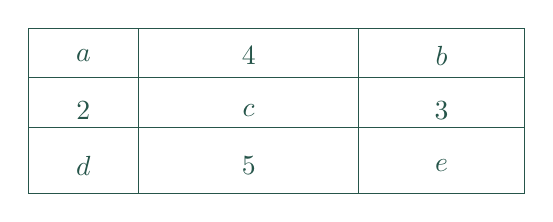
\begin{tikzpicture}[scale=0.7,thachthuctoanhoc]
			\draw (0,0) rectangle (9,3); 
			\draw (2,0) -- (2, 3) (6, 0) -- (6, 3);
			\draw (0,1.2) -- (9, 1.2) (0, 2.1) -- (9, 2.1);
			\draw (1,2.5) node{$a$};
			\draw (1,1.5) node{$2$};
			\draw (1,0.5) node{$d$};
			\draw (4,2.5) node{$4$};
			\draw (4,1.5) node{$c$};
			\draw (4,0.5) node{$5$};
			\draw (7.5,2.5) node{$b$};
			\draw (7.5,1.5) node{$3$};
			\draw (7.5,0.5) node{$e$};
		\end{tikzpicture}
	\end{center}
	\begin{flushright}
		\textit{Đăng Hải, Hà Nội (st)}
	\end{flushright}
	{\color{thachthuctoanhoc}{\usefont{T5}{qag}{b}{n} P672.}}
	(Mức $B$) Cho $x$ và $y$ là các số nguyên dương phân biệt thoả mãn
	\begin{align*}
		2023x^{2023}+999 y^{2023}
	\end{align*}
	chia hết cho $x+y$. Chứng minh rằng $x+y$ là hợp số. 
	\begin{flushright}
		\textit{Nguyễn Đức Tấn, Tp. Hồ Chí Minh}
	\end{flushright}
	{\color{thachthuctoanhoc}{\usefont{T5}{qag}{b}{n} P673.}}
	(Mức $B$) Chứng minh rằng,
	\begin{align*}
		A=\sqrt[3]{1^3+1}+\sqrt[3]{2^3+1}+\cdots+\sqrt[3]{2023^3+1}
	\end{align*}
	không phải là số nguyên.
	\begin{flushright}
		\textit{Nguyễn Văn Quý, Hà Nội}
	\end{flushright}
	{\color{thachthuctoanhoc}{\usefont{T5}{qag}{b}{n} P674.}}
	(Mức $B$) Ở mỗi ô vuông con của bảng ô vuông $8\times8$ được điền một số $+1$, hoặc một số $-1$, sao cho tổng của bốn số ở một bảng con $2\times2$ tuỳ ý bằng $2$, hoặc $-2$. Chứng minh rằng, trong bảng số thu được có hai hàng giống nhau.
	\begin{flushright}
		\textit{Nguyễn Tường Thanh, Nghệ An (st)}
	\end{flushright}
	{\color{thachthuctoanhoc}{\usefont{T5}{qag}{b}{n} P675.}}
	(Mức $B$) Cho hình thang $ABCD$ vuông tại $A$ và $D$. Trên tia $AD$ lấy điểm $F$ sao cho $AF\cdot AD=AB\cdot CD$. Gọi $E$ là hình chiếu vuông góc của $A$ trên $BD$. Chứng minh rằng $\angle CEF=90^\circ$. 
	\begin{figure}[H]
		\vspace*{-15pt}
		\centering
		\captionsetup{labelformat= empty, justification=centering}
		\definecolor{sqsqsq}{rgb}{0.12549019607843137,0.12549019607843137,0.12549019607843137}
		\definecolor{ffqqqq}{rgb}{1,0,0}
		\definecolor{qqzzcc}{rgb}{0,0.6,0.8}
		\definecolor{qqqqff}{rgb}{0,0,1}
		\definecolor{qqqqffa}{rgb}{1,1,1}
		\begin{tikzpicture}[scale=0.5,thachthuctoanhoc, rotate=90]
			\draw[color=sqsqsq] (-3,3.317157287525381) -- (-2.717157287525381,3.317157287525381) -- (-2.717157287525381,3.6) -- (-3,3.6) -- cycle; 
			\draw[color=sqsqsq] (-2.7171572875253815,-3.78) -- (-2.7171572875253815,-3.4971572875253814) -- (-3,-3.4971572875253814) -- (-3,-3.78) -- cycle; 
			\draw[color=sqsqsq] (-0.7031626699615052,2.6414283229649644) -- (-0.8393330759027575,2.315149882755081) -- (-0.5130546356928736,2.1789794768138284) -- (-0.3768842297516215,2.5052579170237124) -- cycle; 
			\draw  (-3,3.6)-- (0.08,3.6);
			\draw  (0.08,3.6)-- (2.48,-3.78);
			\draw [color=qqzzcc] (-3,-3.78)-- (0.08,3.6);
			\draw  (-3,-3.78)-- (2.48,-3.78);
			\draw  (-3,3.6)-- (-3,-3.78);
			\draw [color=ffqqqq] (-3,1.3129539295392954)-- (-0.3768842297516215,2.5052579170237124);
			\draw [color=ffqqqq] (-0.3768842297516215,2.5052579170237124)-- (2.48,-3.78);
			\draw [color=qqzzcc] (-3,3.6)-- (-0.3768842297516215,2.5052579170237124);
			\draw [fill=white] (-3,3.6) circle (1.5pt);
			\draw[color=qqqqff] (-3.04,4.11) node {$A$};
			\draw [fill=white] (0.08,3.6) circle (1.5pt);
			\draw[color=qqqqff] (0.08,4.13) node {$B$};
			\draw [fill=white] (2.48,-3.78) circle (1.5pt);
			\draw[color=qqqqff] (2.9,-3.78) node {$C$};
			\draw [fill=white] (-3,-3.78) circle (1.5pt);
			\draw[color=qqqqff] (-3.6,-3.78) node {$D$};
			\draw [fill=white] (-3,1.3129539295392954) circle (1.5pt);
			\draw[color=qqqqff] (-3.6,1.49) node {$F$};
			\draw [fill=white] (-0.3768842297516215,2.5052579170237124) circle (1.5pt);
			\draw[color=qqqqff] (-0.54,2.99) node {$E$};
		\end{tikzpicture}
		\vspace*{-10pt}
	\end{figure}
	\begin{flushright}
		\textit{Bằng Linh, Phú Thọ}
	\end{flushright}
	{\color{thachthuctoanhoc}{\usefont{T5}{qag}{b}{n} P676.}}
	(Mức $B$) Cho $a, b, c$ là các số thực dương. Chứng minh rằng
	\begin{align*}
		\sqrt{\!\!\frac{a}{b\!+\!c}}\!+\!\sqrt{\!\!\frac{b}{c\!+\!a}}\!+\!\sqrt{\!\!\frac{c}{a\!+\!b}}
		\!\leq\! \sqrt{\!\!\frac{a}{b}\!+\!\frac{b}{c}\!+\!\frac{c}{a}\!+\!\frac{3}{2}} .
	\end{align*}
	\begin{flushright}
		\textit{Nguyễn Việt Hùng, Hà Nội}
	\end{flushright}
	{\color{thachthuctoanhoc}{\usefont{T5}{qag}{b}{n} P677.}}
	(Mức $A$) Cho dãy số thực $(u_n)$ xác định bởi 
	\begin{align*}
		u_n=\dfrac{C^n_{2n}-2022}{n^2}\quad\text{với $n=1,2,3,\ldots$}.
	\end{align*}
	$a)$ Chứng minh rằng $(u_n)$ là dãy tăng và không bị chặn trên.
	\vskip 0.05cm
	$b)$ Tìm tất cả các số thực $\alpha$,  sao cho dãy số $(x_n)$, xác định bởi
	\begin{align*}
		x_n=\dfrac{n^\alpha. u_n}{4^n},\quad n=1,2,3,\ldots,
	\end{align*}
	có giới hạn hữu hạn khác $0$, khi $n\to+\infty$.
	\begin{flushright}
		\textit{Lê Phúc Lữ, Tp. Hồ Chí Minh}
	\end{flushright}
	{\color{thachthuctoanhoc}{\usefont{T5}{qag}{b}{n} P678.}}
	(Mức $A$) Trong mặt phẳng, cho hai điểm $I$, $J$ cố định thoả mãn $IJ=8$.  Gọi $(S)$ là tập hợp các điểm $M$ sao cho ít nhất một trong hai đoạn thẳng $MI,MJ$ có độ dài không vượt quá $7$. Với $A,B,C$ là ba điểm không thẳng hàng thuộc $(S)$, chu vi tam giác $ABC$ lớn nhất là bao nhiêu?
	\begin{flushright}
		\textit{Trần Quốc Luật, Tp. Hồ Chí Minh}
	\end{flushright}
	{\color{thachthuctoanhoc}{\usefont{T5}{qag}{b}{n} P679.}}
	(Mức $A$) Có $100$ quả trứng, được xếp thành một vòng tròn. Gọi một quả bất kỳ, trong $100$ quả trứng đó, là quả thứ nhất; sau đó, theo chiều kim đồng hồ, lần lượt gọi các quả trứng tiếp theo là quả thứ $2$, quả thứ $3$, $\ldots$, quả thứ $100$. Người ta nhặt trứng theo quy tắc: đầu tiên, nhặt quả thứ hai; sau đó, theo chiều kim đồng hồ, cứ cách một quả lại nhặt một quả, cho đến khi nhặt được hết $100$ quả trứng. Hỏi quả trứng nhặt được ở lần cuối cùng là quả thứ mấy?
	\begin{flushright}
		\textit{Phạm Triều Dương, Hà Nội (st)}
	\end{flushright}
	{\color{thachthuctoanhoc}{\usefont{T5}{qag}{b}{n} P680.}}
	(Mức $A$) Xác định tất cả các số nguyên $a$ sao cho: với mỗi số nguyên dương $k$, tồn tại số nguyên dương $n_k$ thoả mãn $2^k\mid n_k^{n_k}+a$. 
	\begin{flushright}
		\textit{Nguyễn Văn Thạch, Đăk Nông}
	\end{flushright}
\end{multicols}
\centerline{{\large{\textbf{\color{thachthuctoanhoc}GIẢI BÀI KỲ TRƯỚC}}}}
\vspace*{-5pt}
\begin{multicols}{2}
	\setlength{\abovedisplayskip}{4pt}
	\setlength{\belowdisplayskip}{4pt}
	{\color{thachthuctoanhoc}{\usefont{T5}{qag}{b}{n} P641.}}
	(Mức $B$)
	Tại mỗi đỉnh của một đa giác lồi $18$ cạnh ở hình dưới đây, người ta ghi một số, sao cho số được ghi ở mỗi đỉnh bằng tổng hai số được ghi ở hai đỉnh kề với nó.
	\begin{figure}[H]
		\vspace*{-5pt}
		\centering
		\captionsetup{labelformat= empty, justification=centering}
		\definecolor{ffvvqq}{rgb}{1,0.3333333333333333,0}
		\definecolor{qqqqffa}{rgb}{0,0,1}
		\definecolor{qqzzff}{rgb}{0,0.6,1}
		\begin{tikzpicture}[line cap=round,line join=round,>=triangle 45,x=1cm,y=1cm,scale=0.4, node font= \small]
			\draw (1.401115339869085,5.50644760016908136) node[anchor=north west] {$X$};
			\draw (1.4408759814898973,-0.7306378725360659) node[anchor=north west] {$Y$};
			\draw (-7.8444170535279,2.5008856260029945) node[anchor=north west] {$S$};
			\draw [color=qqzzff] (0.0915547437082469,-1.9784020259611625)--(1.3147607160299626,-0.9781184915188108);
			\draw [color=qqzzff] (1.3147607160299626,-0.9781184915188108)--(2.122081224105652,0.3802016464606015); 
			\draw [color=qqzzff] (2.122081224105652,0.3802016464606015)--(2.4161414998796458,1.932724932666551); 
			\draw [color=qqzzff] (2.4161414998796458,1.932724932666551)--(2.1614735342261406,3.4921941459791768);
			\draw [color=qqzzff] (2.1614735342261406,3.4921941459791768)--(1.38879404230183,4.87051428395859);
			\draw [color=qqzzff] (1.38879404230183,4.87051428395859)--(0.19129957436757605,5.901439596125702);
			\draw [color=qqzzff] (0.19129957436757605,5.901439596125702)--(-1.2865743636076452,6.4606252749959765);
			\draw [color=qqzzff] (-1.2865743636076452,6.4606252749959765)--(-2.866574363607645,6.480625274995977);
			\draw [color=qqzzff] (-2.866574363607645,6.480625274995977)--(-4.358129107315893,5.959027300957139);
			\draw [color=qqzzff] (-4.358129107315893,5.959027300957139)--(-5.581335079637608,4.958743766514788);
			\draw [color=qqzzff] (-5.581335079637608,4.958743766514788)--(-6.388655587713298,3.600423628535374);
			\draw [color=qqzzff] (-6.388655587713298,3.600423628535374)--(-6.682715863487291,2.0479003423294264);
			\draw [color=qqzzff] (-6.682715863487291,2.0479003423294264)--(-6.428047897833785,0.4884311290167975);
			\draw [color=qqzzff] (-6.428047897833785,0.4884311290167975)--(-5.655368405909476,-0.889889008962613);
			\draw [color=qqzzff] (-5.655368405909476,-0.889889008962613)--(-4.457873937975224,-1.9208143211297237);
			\draw [color=qqzzff] (-4.457873937975224,-1.9208143211297237)--(-2.98,-2.48);
			\draw [color=qqzzff] (-2.98,-2.48)--(-1.4,-2.5);
			\draw [color=qqzzff] (-1.4,-2.5)--(0.0915547437082469,-1.9784020259611625);
			\draw [fill=white] (-2.98,-2.48) circle (1.6pt);
			\draw [fill=white] (-1.4,-2.5) circle (1.6pt);
			\draw [fill=white] (0.0915547437082469,-1.9784020259611625) circle (1.6pt);
			\draw [fill=white] (1.3147607160299626,-0.9781184915188108) circle (1.6pt);
			\draw [fill=white] (2.122081224105652,0.3802016464606015) circle (1.6pt);
			\draw [fill=white] (2.4161414998796458,1.932724932666551) circle (1.6pt);
			\draw [fill=white] (2.1614735342261406,3.4921941459791768) circle (1.6pt);
			\draw [fill=white] (1.38879404230183,4.87051428395859) circle (1.6pt);
			\draw [fill=white] (0.19129957436757605,5.901439596125702) circle (1.6pt);
			\draw [fill=white] (-1.2865743636076452,6.4606252749959765) circle (1.6pt);
			\draw [fill=white] (-2.866574363607645,6.480625274995977) circle (1.6pt);
			\draw [fill=white] (-4.358129107315893,5.959027300957139) circle (1.6pt);
			\draw [fill=white] (-5.581335079637608,4.958743766514788) circle (1.6pt);
			\draw [fill=white] (-6.388655587713298,3.600423628535374) circle (1.6pt);
			\draw [fill=white] (-6.682715863487291,2.0479003423294264) circle (1.6pt);
			\draw [fill=white] (-6.428047897833785,0.4884311290167975) circle (1.6pt);
			\draw [fill=white] (-5.655368405909476,-0.889889008962613) circle (1.6pt);
			\draw [fill=white] (-4.457873937975224,-1.9208143211297237) circle (1.6pt);
		\end{tikzpicture}
		\vspace*{-5pt}
	\end{figure}
	Biết rằng, số được ghi ở đỉnh $X$ là $20$, và số được ghi ở đỉnh $Y$ là $22$. Hãy tìm số được ghi ở đỉnh $S$.
	\vskip 0.05cm
	\textbf{\color{thachthuctoanhoc}Lời giải} (\textit{phỏng theo ý giải của bạn Nguyễn Chánh Thiện, lớp $8/14$, trường THCS Lê Quý Đôn, Quận $3$, Tp. Hồ Chí Minh})\textbf{\color{thachthuctoanhoc}.}
	\vskip 0.05cm
	Xuất phát từ đỉnh $S$, theo chiều kim đồng hồ, ký hiệu các số được ghi tại các đỉnh của $18$--giác, lần lượt, bởi  $x_1,  x_2, \ldots, x_{18}$ (xem Hình dưới đây).
	\vskip 0.05cm
	Do $x_8$, $x_{12}$ là các số được ghi tại các đỉnh $X$, $Y$, nên theo giả thiết của bài ra, $x_8 =20$  và  $x_{12} = 22$.
	\begin{figure}[H]
		\centering
		\vspace*{-10pt}
		\captionsetup{labelformat= empty, justification=centering}
		\includegraphics[width=0.7\linewidth]{P641}
		\vspace*{-10pt}
	\end{figure}
	Từ quy tắc ghi số của đề bài suy ra, với mỗi $k = 1, 2, \ldots, 15$, ta có:
	\begin{align*}
		{x_k} &= {x_{k + 1}} - {x_{k + 2}} = {x_{k + 1}} - \left( {{x_{k + 1}} + {x_{k + 3}}} \right) \\
		&=  - {x_{k + 3}}.
	\end{align*}
	Do đó
	\begin{align*}
		&{x_2} =  - {x_5} = {x_8} = 20,\\
		&22 = {x_{12}} =  - {x_{15}} = {x_{18}}.
	\end{align*}
	Vì vậy
	\begin{align*}
		{x_1} = {x_{18}} + {x_2} = 22 + 20 = 42.
	\end{align*}
	Vậy, số được ghi ở đỉnh $S$ là $42$.
	\vskip 0.05cm
	\textbf{\color{thachthuctoanhoc}Bình luận và Nhận xét}
	\vskip 0.05cm	
	Tạp chí đã nhận được nhiều lời giải cho bài toán, từ bạn đọc; và tất cả những lời giải này đều là lời giải đúng.
	\vskip 0.1cm
	\hfill	\textbf{\color{thachthuctoanhoc}Lê Huy}
	\vskip 0.1cm
	{\color{thachthuctoanhoc}{\usefont{T5}{qag}{b}{n} P642.}}
	(Mức $B$)
	Cho $x$, $y$ là các số nguyên dương thỏa mãn $y^2 \!+\! x \!-\! 1$ chia hết cho $xy \!+\! 1$. Chứng minh rằng, tồn tại số tự nhiên $z$, sao cho $x + y + z + xyz$ là một số chính phương.
	\vskip 0.05cm
	\textbf{\color{thachthuctoanhoc}Lời giải} (\textit{của người đề xuất bài toán})\textbf{\color{thachthuctoanhoc}.}
	\vskip 0.05cm
	Từ giả thiết của bài toán, suy ra
	\begin{align*}
		&{xy + 1} \mid x\left( {{y^2} + x - 1} \right) \\
		= &y\left( {xy + 1} \right) + \left( {{x^2} - \left( {x + y} \right)} \right).
	\end{align*}
	Do đó
	\begin{align*}
		{xy + 1} \mid {x^2} - \left( {x + y} \right).
	\end{align*}
	Vì thế, tồn tại số nguyên $z$, sao cho
	\begin{align*}
		{x^2} - \left( {x + y} \right) = z\left( {xy + 1} \right);
	\end{align*}
	hay, $x + y + z + xyz = {x^2}.$
	\vskip 0.05cm  
	Nhận thấy, nếu $z \le -1$  thì
	\begin{align*}
		{x^2} &= x + y + z + xyz \le x + y - 1 - xy \\
		&= - \left( {x - 1} \right)\left( {y - 1} \right) \le 0,
	\end{align*}
	là điều vô lý (do  $x \in \mathbb{N^*}$).
	\vskip 0.05cm
	Vì vậy, $z \ge 0$; hay, $z$ là số tự nhiên.
	\vskip 0.05cm
	Vậy, tồn tại số tự nhiên $z$, sao cho 
	\begin{align*}
		x + y + z + xyz
	\end{align*} là một số chính phương.
	\vskip 0.05cm
	\textbf{\color{thachthuctoanhoc}Bình luận và Nhận xét}
	\vskip 0.05cm
	$\pmb{1.}$ Tác giả bài toán đã chứng minh được rằng, nếu $z_0$  là một số tự nhiên, sao cho $x + y + z_0 + xyz_0$  là một số chính phương, thì tất cả các số tự nhiên $z_k, k \in \mathbb{N^*}$, xác định bởi
	\begin{align*}
		{z_k} = {z_0} + 2xk + \left( {xy + 1} \right){k^2},
	\end{align*}
	cũng có tính chất như vậy. Vì thế, kết luận của bài ra có thể được mở rộng thành: “Có vô số số tự nhiên $z$, sao cho $x + y + z + xyz$ là một số chính phương.”
	\vskip 0.05cm
	$\pmb{2.}$ Theo ý giải của bạn \textit{Vương Khánh Toàn} (lớp $10$A$1$ Toán, trường THPT chuyên KHTN, trường ĐHKHTN, ĐHQG Hà Nội), có thể chứng minh được rằng, các số nguyên dương $x$, $y$ thỏa mãn điều kiện của bài ra khi và chỉ khi $x = k + 1, y = k(k + 1)$, trong đó, $k$ là một số nguyên dương tùy ý. Từ đây, dễ thấy, chọn $z = 0$, ta sẽ có số tự nhiên $z$ thỏa mãn yêu cầu đề bài.
	\vskip 0.05cm
	$\pmb{3.}$ Rất tiếc, trong số các lời giải Tạp chí đã nhận được từ bạn đọc, có một số lời giải sai, do người giải bài đã mắc một trong các lỗi sau đây:
	\vskip 0.05cm
	-- \textit{Ngộ nhận} rằng, không mất tính tổng quát, có thể giả sử $x^2 > x + y$;
	\vskip 0.05cm 
	-- \textit{Hiểu sai} rằng, số nguyên $a$ chia hết cho số nguyên $b$ khi và chỉ khi tồn tại số \textit{tự nhiên} $q$, sao cho $a = bq$;
	\vskip 0.05cm
	--\textit{ Suy luận sai} rằng, với $x$, $y$ là các số nguyên dương, và $a$ là số nguyên âm, từ
	\begin{align*}
		{x^2} - x - y = a\left( {xy + 1} \right)
	\end{align*}
	suy ra, $x^2 - x - y = 0$.
	\vskip 0.05cm  
	Cùng với các lời giải sai nêu trên, có một lời giải không được coi là lời giải hoàn chỉnh, do các lập luận thiếu chặt chẽ, thiếu chính xác.
	\begin{flushright}
		\textbf{\color{thachthuctoanhoc}Lưu Thị Thanh Hà}
	\end{flushright}
	{\color{thachthuctoanhoc}{\usefont{T5}{qag}{b}{n} P643.}}
	(Mức $B$)
	Người ta lần lượt ghi các số lên bảng, theo quy tắc: Ở mỗi lần ghi, chỉ ghi một số, và nếu số được ghi ở lần thứ $k$ ($k \in \mathbb{N^*}$) là $x \ne -1$,  thì ở lần thứ $k + 1$ ghi số $\dfrac{x-1}{x+1}$. Hãy tìm số nhỏ nhất cần ghi ở lần thứ nhất, sao cho trong quá trình ghi số lên bảng theo quy tắc trên, ta ghi được số $-\dfrac{1}{2023}$.
	\vskip 0.05cm
	\textbf{\color{thachthuctoanhoc}Lời giải} (\textit{của người chấm bài})\textbf{\color{thachthuctoanhoc}.}
	\vskip 0.05cm
	Với mỗi $k \in \mathbb{N^*}$,  ký hiệu $x_k$  là số được ghi lên bảng ở lần ghi thứ $k$.
	\vskip 0.05cm
	Gọi $a$ là số được ghi lên bảng ở lần ghi đầu tiên; ta có $x_1 = a$.
	\vskip 0.05cm 
	Theo quy tắc ghi số của bài ra, để có thể ghi tiếp một số mới lên bảng, cần có $a \ne -1$.  Khi đó, ta có
	\begin{align*}
		{x_2} = \frac{{a - 1}}{{a + 1}}.
	\end{align*}
	Dễ thấy, $x_2 \ne -1$   khi và chỉ khi $a \ne 0$. Do đó, với $a \ne 0 ,-1$,   ta có
	\begin{align*}
		{x_3} = \frac{{{x_2} - 1}}{{{x_2} + 1}} =  - \frac{1}{a}.
	\end{align*}
	Vì $x_3 \ne -1$ khi và chỉ khi $a \ne 1$, nên với $a \ne 0, \pm 1$  ta có:
	\begin{align*}
		{x_4} = \frac{{{x_3} - 1}}{{{x_3} + 1}} =  - \frac{{a + 1}}{{a - 1}}.
	\end{align*}
	Do $x_4 \ne -1$ với mọi $a$, nên
	\begin{align*}
		{x_5} = \frac{{{x_4} - 1}}{{{x_4} + 1}} = a = {x_1}.
	\end{align*}
	Từ những điều nêu trên, suy ra:
	\vskip 0.05cm
	-- Nếu $a = -1$  thì ta ghi được lên bảng duy nhất số $-1$.
	\vskip 0.05cm 
	-- Nếu $a = 0$ thì ta ghi được lên bảng hai số, là $0$ và $-1$.
	\vskip 0.05cm 
	-- Nếu $a = 1$ thì ta ghi được lên bảng ba số, là $1$, $0$ và $-1$.
	\vskip 0.05cm 
	-- Nếu $a\ne 0, \pm 1$,  thì tất cả các số ghi được lên bảng là $a, \dfrac{a-1}{a+1}, -\dfrac{1}{a}, -\dfrac{a+1}{a-1}$.
	\vskip 0.05cm      
	Vì vậy, ta ghi được lên bảng số $-\dfrac{1}{2023}$  khi và chỉ khi $a \ne 0, \pm 1$, và đồng thời, một trong bốn số vừa nêu trên bằng $-\dfrac{1}{2023}$.
	\vskip 0.05cm
	Ta có:
	\begin{align*}
		\frac{{a - 1}}{{a + 1}} =  - \frac{1}{{2023}}& \Leftrightarrow a = \frac{1011}{1012};\\
		-\dfrac{1}{a} = - \frac{1}{2023} &\Leftrightarrow a = 2023;\\
		-\dfrac{a +1}{a-1} = -\dfrac{1}{2023} &\Leftrightarrow a = - \dfrac{1012}{1011}.
	\end{align*}
	Do đó, ta ghi được lên bảng số $-\dfrac{1}{2023}$  khi và chỉ khi $a \in \left\{ { - \dfrac{1}{{2023}};\dfrac{{1011}}{{1012}};2023; - \dfrac{{1012}}{{1011}}} \right\}$.   Dễ thấy,  $-\dfrac{1012}{1011}$ là số nhỏ nhất trong bốn số thuộc tập hợp vừa nêu. Vì vậy, số nhỏ nhất cần ghi ở lần đầu tiên, sao cho có thể ghi lên bảng số  $-\dfrac{1}{2023}$, là  $-\dfrac{1012}{1011}$.
	\vskip 0.1cm
	\textbf{\color{thachthuctoanhoc}Bình luận và Nhận xét}
	\vskip 0.1cm
	$\pmb{1.}$ Xét về logic, trong quy tắc ghi số của bài ra, cần nêu rõ, nếu số được ghi lên bảng là $-1$ thì việc ghi số sẽ tiếp tục thế nào? Dừng lại, không ghi số nữa, hay ghi tiếp số nào? Lời giải trên đây là lời giải dựa trên việc hiểu quy tắc ghi số của bài ra, theo hướng: Việc ghi số lên bảng sẽ dừng lại, ngay sau khi số được ghi là $-1$.
	\vskip 0.05cm
	$\pmb{2.}$ Rất tiếc, tất cả các lời giải Tạp chí nhận được từ bạn đọc đều không được coi là lời giải hoàn chỉnh, do người giải bài đã khẳng định \textit{không đúng} rằng, với $a$ (theo ký hiệu trong Lời giải trên) là số tùy ý, các số ghi được lên bảng \textit{luôn là} $a, \dfrac{a-1}{a+1}, - \dfrac{1}{a}, - \dfrac{a+1}{a-1}$.      
	\begin{flushright}
		\textbf{\color{thachthuctoanhoc}Hà Thanh}
	\end{flushright}
	{\color{thachthuctoanhoc}{\usefont{T5}{qag}{b}{n} P644.}}
	(Mức $B$)
	Xét tam giác $ABC$ có các góc $B$, $C$ nhọn. Gọi $H$ là chân đường cao kẻ từ $A$ của tam giác đó. Chứng minh rằng $ABC$ là tam giác vuông tại $A$ khi và chỉ khi
	\begin{align*}
		\frac{{H{B^3}}}{{A{B^4}}} + \frac{{H{C^3}}}{{A{C^4}}} = \frac{1}{{BC}}.
	\end{align*}
	\textbf{\color{thachthuctoanhoc}Lời giải} (\textit{dựa theo lời giải của bạn Vũ Bảo Lân, lớp $8$A$5$, trường THCS Phúc Yên, Tp. Phúc Yên, tỉnh Vĩnh Phúc})\textbf{\color{thachthuctoanhoc}.}
	\vskip 0.05cm
	$\pmb{1.}$ \textit{Chứng minh “chỉ khi”.
		\vskip 0.05cm
		Giả sử tam giác $ABC$ vuông tại} $A$ (xem Hình $1$) .\textit{Ta cần chứng minh}
	\begin{align*}
		\frac{{H{B^3}}}{{A{B^4}}} + \frac{{H{C^3}}}{{A{C^4}}} = \frac{1}{{BC}}. \tag{$1$}
	\end{align*}                                                           
	\begin{figure}[H]
		\centering
		\vspace*{-5pt}
		\captionsetup{labelformat= empty, justification=centering}
		\begin{tikzpicture}[scale=0.6,thachthuctoanhoc]
			\draw[] (2.8557926412572288,2.657631836505606) -- (3.07873080533295,2.4835669779081666) -- (3.2527956639303897,2.7065051419838877) -- (3.029857499854668,2.8805700005813275) -- cycle; 
			\draw[] (3.312700212329287,-1.) -- (3.312700212329287,-0.7171572875253811) -- (3.029857499854668,-0.7171572875253811) -- (3.029857499854668,-1.) -- cycle; 
			\draw [] (0.,-1.)-- (8.,-1.);
			\draw [] (3.029857499854668,2.8805700005813275)-- (0.,-1.);
			\draw [] (3.029857499854668,2.8805700005813275)-- (8.,-1.);
			\draw [] (3.029857499854668,-1.)-- (3.029857499854668,2.8805700005813275);
			\draw (2.78,3.85) node[anchor=north west] {$A$};
			\draw (-0.48,-0.95) node[anchor=north west] {$B$};
			\draw (7.85,-0.95) node[anchor=north west] {$C$};
			\draw (2.72,-0.95) node[anchor=north west] {$H$};
			\draw [fill=white] (0.,-1.) circle (1.5pt);
			\draw [fill=white] (8.,-1.) circle (1.5pt);
			\draw [fill=white] (3.029857499854668,2.8805700005813275) circle (1.5pt);
			\draw [fill=white] (3.029857499854668,-1.) circle (1.5pt);
		\end{tikzpicture}
		\caption{\small\textit{\color{thachthuctoanhoc}Hình $1$.}}
		\vspace*{-10pt}
	\end{figure}
	Do $H$ là chân đường cao kẻ từ đỉnh góc vuông của tam giác vuông $ABC$ nên
	\begin{align*}
		A{B^2} = &BC \cdot BH, \,\,\,AC^2 = BC \cdot CH,\\
		&\text{và }	BC = HB + HC.
	\end{align*}
	Do đó
	\begin{align*}
		\frac{{H{B^3}}}{{A{B^4}}} + \frac{{H{C^3}}}{{A{C^4}}} &= \frac{{H{B^3}}}{{B{C^2} \cdot H{B^2}}} + \frac{{H{C^3}}}{{B{C^2} \cdot H{C^2}}} \\
		&= \frac{{HB + HC}}{{B{C^2}}} = \frac{1}{{BC}}.
	\end{align*}
	($1$) được chứng minh.
	\vskip 0.05cm
	$\pmb{2.}$ \textit{Chứng minh “khi”.
		\vskip 0.05cm
		Giả sử $ABC$ là tam giác thỏa mãn ($1$), và có các góc $B$, $C$ là góc nhọn. 
		Ta cần chứng minh tam giác $ABC$ vuông tại $A$.}
	Gọi $A'$ là giao điểm của tia $HA$ và đường tròn đường kính $BC$; ta có $\angle BA'C = 90^\circ$,  và $H$ là chân đường cao kẻ từ $A'$  của tam giác vuông $A'BC$. Do đó, theo chứng minh ở phần $1$, ta có:
	\begin{align*}
		\frac{{H{B^3}}}{{A'{B^4}}} + \frac{{H{C^3}}}{{A'{C^4}}} = \frac{1}{{BC}}. \tag{$2$}	
	\end{align*}
	Nhận thấy:
	\vskip 0.05cm
	-- Nếu góc $A$ là góc nhọn (xem Hình $2$) thì điểm $A$ nằm bên ngoài đường tròn đường kính $BC$.
	\begin{figure}[H]
		\centering
		%		\vspace*{-5pt}
		\captionsetup{labelformat= empty, justification=centering}
		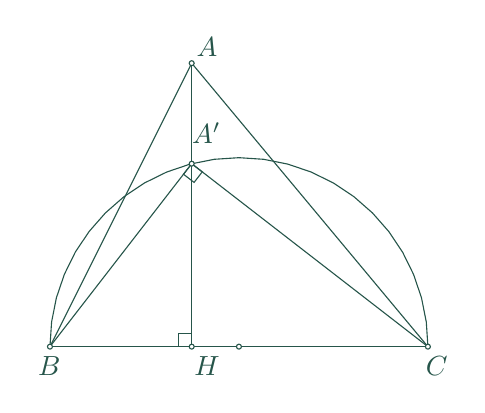
\begin{tikzpicture}[scale=0.6,thachthuctoanhoc]
			\draw[] (2.,0.28284271247461906) -- (1.7171572875253809,0.28284271247461906) -- (1.7171572875253809,0.) -- (2.,0.) -- cycle; 
			\draw[] (1.8267949192431123,3.6493765484574374) -- (2.0504017169930915,3.4761714677005497) -- (2.223606797749979,3.699778265450529) -- (2.,3.8729833462074166) -- cycle; 
			\draw [] (-1.,0.)-- (7.,0.);
			\draw [] (2.,3.8729833462074166)-- (-1.,0.);
			\draw [] (2.,3.8729833462074166)-- (7.,0.);
			\draw [] (2.,6.)-- (-1.,0.);
			\draw [] (2.,6.)-- (7.,0.);
			\draw [] (2.,0.)-- (2.,6.);
			\draw [shift={(3.,0.)},]  plot[domain=0.:3.141592653589793,variable=\t]({1.*4.*cos(\t r)+0.*4.*sin(\t r)},{0.*4.*cos(\t r)+1.*4.*sin(\t r)});
			\draw (1.9,6.74) node[anchor=north west] {$A$};
			\draw (-1.46,0) node[anchor=north west] {$B$};
			\draw (6.75,0) node[anchor=north west] {$C$};
			\draw (1.85,0) node[anchor=north west] {$H$};
			\draw (1.8,4.95) node[anchor=north west] {$A'$};
			\draw [fill=white] (-1.,0.) circle (1.5pt);
			\draw [fill=white] (7.,0.) circle (1.5pt);
			\draw [fill=white] (3.,0.) circle (1.5pt);
			\draw [fill=white] (2.,0.) circle (1.5pt);
			\draw [fill=white] (2.,3.8729833462074166) circle (1.5pt);
			\draw [fill=white] (2.,6.) circle (1.5pt);
		\end{tikzpicture}
		\caption{\small\textit{\color{thachthuctoanhoc}Hình $2$.}}
		\vspace*{-10pt}
	\end{figure}
	Vì thế, điểm $A'$ nằm giữa hai điểm $H$, $A$. Suy ra, $AB > A'B$  và $AC > A'C$.  Do đó, với lưu ý tới ($2$), ta có:
	\begin{align*}
		\frac{{H{B^3}}}{{A{B^4}}} + \frac{{H{C^3}}}{{A{C^4}}} < \frac{{H{B^3}}}{{A'{B^4}}} + \frac{{H{C^3}}}{{A'{C^4}}} = \frac{1}{{BC}},
	\end{align*}
	mâu thuẫn với ($1$). Vì vậy, góc $A$ không thể là góc nhọn.                     \hfill ($3$)
	\vskip 0.05cm
	-- Nếu góc $A$ là góc tù (xem Hình $3$) thì điểm $A$ nằm bên trong đường tròn đường kính $BC$.
	\begin{figure}[H]
		\centering
		\vspace*{-5pt}
		\captionsetup{labelformat= empty, justification=centering}
		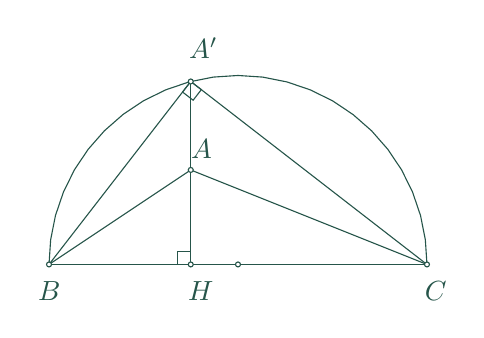
\begin{tikzpicture}[scale=0.6,thachthuctoanhoc]
			\draw[] (1.8267949192431123,4.649376548457438) -- (2.0504017169930915,4.47617146770055) -- (2.223606797749979,4.699778265450529) -- (2.,4.872983346207417) -- cycle; 
			\draw[] (2.,1.2828427124746191) -- (1.7171572875253809,1.2828427124746191) -- (1.7171572875253809,1.) -- (2.,1.) -- cycle; 
			\draw [] (-1.,1.)-- (7.,1.);
			\draw [] (2.,3.)-- (-1.,1.);
			\draw [] (2.,3.)-- (7.,1.);
			\draw [shift={(3.,1.)},]  plot[domain=0.:3.141592653589793,variable=\t]({1.*4.*cos(\t r)+0.*4.*sin(\t r)},{0.*4.*cos(\t r)+1.*4.*sin(\t r)});
			\draw [] (2.,4.872983346207417)-- (-1.,1.);
			\draw [] (2.,4.872983346207417)-- (7.,1.);
			\draw [] (2.,1.)-- (2.,4.872983346207417);
			\draw (1.76,6) node[anchor=north west] {$A'$};
			\draw (1.8,3.85) node[anchor=north west] {$A$};
			\draw (-1.44,0.85) node[anchor=north west] {$B$};
			\draw (1.74,0.85) node[anchor=north west] {$H$};
			\draw (6.75,0.85) node[anchor=north west] {$C$};
			\draw [fill=white] (-1.,1.) circle (1.5pt);
			\draw [fill=white] (7.,1.) circle (1.5pt);
			\draw [fill=white] (3.,1.) circle (1.5pt);
			\draw [fill=white] (2.,1.) circle (1.5pt);
			\draw [fill=white] (2.,4.872983346207417) circle (1.5pt);
			\draw [fill=white] (2.,3.) circle (1.5pt);
		\end{tikzpicture}
		\caption{\small\textit{\color{thachthuctoanhoc}Hình $3$.}}
		\vspace*{-10pt}
	\end{figure}
	Vì thế, điểm $A$ nằm giữa hai điểm $H, A'$. Suy ra, $AB < A'B$ và $AC < A'C$.  Do đó, với lưu ý tới ($2$), ta có:
	\begin{align*}
		\frac{{H{B^3}}}{{A{B^4}}} + \frac{{H{C^3}}}{{A{C^4}}} > \frac{{H{B^3}}}{{A'{B^4}}} + \frac{{H{C^3}}}{{A'{C^4}}} = \frac{1}{{BC}},
	\end{align*}
	mâu thuẫn với ($1$). Vì vậy, góc $A$ không thể là góc tù.  \hfill ($4$)
	\vskip 0.05cm
	Từ ($3$) và ($4$) suy ra, góc $A$ là góc vuông; và do đó, ta có điều cần chứng minh.
	\vskip 0.05cm
	\textbf{\color{thachthuctoanhoc}Bình luận và Nhận xét}
	\vskip 0.05cm
	Rất tiếc, trong số các lời giải Tạp chí đã nhận được từ bạn đọc, có một số lời giải sai, do người giải bài đã mắc một trong các lỗi sau:
	\vskip 0.05cm
	-- \textit{Mới chỉ chứng minh được}, nếu tam giác $ABC$ vuông tại $A$ thì ta có hệ thức đã nêu trong đề bài;
	\vskip 0.05cm
	-- \textit{Ngộ nhận} rằng, hiển nhiên có
	\begin{align*}
		&HB\!\left(\!\!\!\frac{{H{B^2}}}{{A{B^4}}} \!-\! \frac{1}{{B{C^2}}}\!\!\! \right)\!\!+\! HC \! \left(\!\!\!\frac{{H{C^2}}}{{A{C^4}}} \!-\! \frac{1}{{B{C^2}}} \!\!\!\right) \!\!=\! 0\\
		\Leftrightarrow &\frac{{H{B^2}}}{{A{B^4}}} - \frac{1}{{B{C^2}}} = \frac{{H{C^2}}}{{A{C^4}}} - \frac{1}{{B{C^2}}} = 0.
	\end{align*}
	\begin{flushright}
		\textbf{\color{thachthuctoanhoc}Hạ Vũ Anh}
	\end{flushright}
	{\color{thachthuctoanhoc}{\usefont{T5}{qag}{b}{n} P645.}}
	(Mức $B$)
	Cho $a$, $b$, $c$ là các số thực dương thỏa mãn $abc = 1$. Chứng minh rằng
	\begin{align*}
		\frac{a}{{a \!+ \!{b^3}c \!+\! b}} \!+\! \frac{b}{{b \!+\! {c^3}a \!+\! c}} \!+\! \frac{c}{{c \!+\! {a^3}b \!+\! a}} \ge 1.
	\end{align*}
	\textbf{\color{thachthuctoanhoc}Lời giải} (\textit{dựa theo lời giải của người đề xuất bài toán})\textbf{\color{thachthuctoanhoc}.}
	\vskip 0.05cm
	Do $abc = 1$ nên
	\begin{align*}
		\frac{a}{{a \!+\! {b^3}c \!+\! b}} \!=\! \frac{{{a^2}}}{{{a^2} \!+\! a{b^3}c \!+\! ab}} \!=\! \frac{{{a^2}}}{{{a^2} \!+\! ab \!+\! {b^2}}}.
	\end{align*}
	Bằng cách hoàn toàn tương tự, ta có:
	\begin{align*}
		&\frac{b}{{b + {c^3}a + c}} = \frac{{{b^2}}}{{{b^2} + bc + {c^2}}},\\ &\frac{c}{{c + {a^3}b + a}} = \frac{{{c^2}}}{{{c^2} + ca + {a^2}}}.
	\end{align*}
	Do đó, bất đẳng thức cần chứng minh của đề bài tương đương với bất đẳng thức
	\begin{align*}
		&\frac{{{a^2}}}{{{a^2} + ab + {b^2}}} + \frac{{{b^2}}}{{{b^2} + bc + {c^2}}} \\
		&+ \frac{{{c^2}}}{{{c^2} + ca + {a^2}}} \ge 1. \tag{$1$}
	\end{align*}
	Theo bất đẳng thức Cauchy -- Schwarz cho hai số thực dương, ta có:
	\begin{align*}
		&\frac{{{a^2}}}{{{a^2} + ab + {b^2}}} + \frac{c}{{a + b + c}} \\
		= &\frac{{{a^2}}}{{{a^2} + ab + {b^2}}} + \frac{{{c^2}}}{{ac + bc + {c^2}}} \\
		\ge &\frac{{{{\left( {a + c} \right)}^2}}}{{{a^2} + {b^2} + {c^2} + ab + bc + ca}}. \tag{$2$}
	\end{align*}
	Bằng cách hoàn toàn tương tự, ta cũng chứng minh được:
	\begin{align*}
		&\frac{{{b^2}}}{{{b^2} + bc + {c^2}}} + \frac{a}{{a + b + c}} \\
		\ge &\frac{{{{\left( {b + a} \right)}^2}}}{{{a^2} + {b^2} + {c^2} + ab + bc + ca}} \tag{$3$}\\
		&\frac{{{c^2}}}{{{c^2} + ca + {a^2}}} + \frac{b}{{a + b + c}} \\
		\ge &\frac{{{{\left( {c + b} \right)}^2}}}{{{a^2} + {b^2} + {c^2} + ab + bc + ca}}. \tag{$4$}
	\end{align*}
	Cộng các bất đẳng thức ($2$), ($3$), ($4$), vế theo vế, ta được:
	\begin{align*}
		&\frac{{{a^2}}}{{{a^2}+ ab + {b^2}}} + \frac{{{b^2}}}{{{b^2} + bc + {c^2}}} \\
		&+ \frac{{{c^2}}}{{{c^2} + ca + {a^2}}} + 1\\[+1ex]
		\ge &\frac{{{{\left( {a + c} \right)}^2} + {{\left( {b + a} \right)}^2} + {{\left( {c + b} \right)}^2}}}{{{a^2} + {b^2} + {c^2} + ab + bc + ca}}\\[+1ex]
		= &\frac{{2\left( {{a^2} + {b^2} + {c^2} + ab + bc + ca} \right)}}{{{a^2} + {b^2} + {c^2} + ab + bc + ca}} = 2.
	\end{align*}
	Suy ra
	\begin{align*}
		&\frac{{{a^2}}}{{{a^2} + ab + {b^2}}} + \frac{{{b^2}}}{{{b^2} + bc + {c^2}}} \\
		&+ \frac{{{c^2}}}{{{c^2} + ca + {a^2}}} \ge 1.
	\end{align*}
	Bất đẳng thức ($1$) được chứng minh; và do đó, bất đẳng thức của đề bài được chứng minh.
	\vskip 0.05cm
	\textbf{\color{thachthuctoanhoc}Bình luận và Nhận xét}
	\vskip 0.05cm
	$\pmb{1.}$ Từ Lời giải trên dễ thấy, bất đẳng thức của bài ra là một biến thể đơn sơ, nhẹ nhàng của bất đẳng thức ($1$).
	\vskip 0.05cm
	$\pmb{2.}$ Bất đẳng thức ($1$) là một bất đẳng thức đã có từ lâu. Tác giả Vasile Cirtoaje đã giới thiệu bất đẳng thức này trong cuốn sách “\textit{Algebraic Inequalities: Old and New Method}” (bài số $10$, trang $21$), do Nhà xuất bản GIL phát hành năm $2006$. Trong cuốn sách này, Vasile Cirtoaje đã giới thiệu một cách chứng minh rất độc đáo cho bất đẳng thức đó,  như sau:
	\vskip 0.05cm
	“Đặt $x = {a^2} + ab + {b^2},$ $y = {b^2} + bc + {c^2},$      và $z = {c^2} + ca + {a^2}$.  Ta có:
	\begin{align*}
		&\left( {\frac{1}{x} + \frac{1}{y} + \frac{1}{z}} \right)\left( {\frac{{{a^2}}}{x} + \frac{{{b^2}}}{y} + \frac{{{c^2}}}{z}} \right)\\
		= &\frac{{{a^2}}}{{{x^2}}} \!+\! \frac{{{b^2}}}{{{y^2}}} \!+\! \frac{{{c^2}}}{{{z^2}}} \!+\! \frac{{{a^2} \!+\! {b^2}}}{{xy}} \!+\! \frac{{{b^2} \!+\! {c^2}}}{{yz}} \!+\! \frac{{{c^2} \!+\! {a^2}}}{{zx}}\\
		\ge &\frac{{ab}}{{xy}} \!+\! \frac{{bc}}{{yz}} \!+\! \frac{{ca}}{{zx}} \!+\! \frac{{{a^2} \!+\! {b^2}}}{{xy}} \!+\! \frac{{{b^2} \!+\! {c^2}}}{{yz}} \!+\! \frac{{{c^2}\! +\! {a^2}}}{{zx}}\\
		= &\frac{1}{y} + \frac{1}{z} + \frac{1}{x}.
	\end{align*}
	Từ đó, hiển nhiên thu được bất đẳng thức ($1$).”
	\vskip 0.05cm
	$\pmb{3.}$ Rất tiếc, trong số các lời giải Tạp chí đã nhận được từ bạn đọc, có hai lời giải sai, do người giải bài đã mắc một trong các lỗi sau:
	\vskip 0.05cm
	-- \textit{Thực hiện sai một số biến đổi}; chẳng hạn:
	\begin{align*}
		\frac{{{a^2}}}{{{a^2} + ab + {b^2}}} = {a^2}\left( {1 - \frac{{ab + {b^2}}}{{{a^2} + ab + {b^2}}}} \right).
	\end{align*}
	-- \textit{Nhầm chiều bất đẳng thức}; chẳng hạn:
	\begin{align*}
		&\frac{{{{\left( {a + b + c} \right)}^2}}}{{{{\left( {a \!+\! b \!+\! c} \right)}^2} \!+\! \left( {{a^2} \!+\! {b^2} \!+\! {c^2} \!-\! ab \!-\! bc \!-\! ca} \right)}} \\
		\ge &\frac{{{{\left( {a + b + c} \right)}^2}}}{{{{\left( {a + b + c} \right)}^2}}}.
	\end{align*}
	\begin{flushright}
		\textbf{\color{thachthuctoanhoc}Võ Quốc Bá Cẩn}
	\end{flushright}
	{\color{thachthuctoanhoc}{\usefont{T5}{qag}{b}{n} P646.}}
	(Mức $B$)
	Chứng minh rằng, trong mỗi bát giác lồi, luôn có ít nhất ba đường chéo mà độ dài của chúng đôi một khác nhau.
	(Bát giác là một đa giác có $8$ cạnh.)
	\vskip 0.05cm
	\textbf{\color{thachthuctoanhoc}Lời giải} (\textit{của người chấm bài})\textbf{\color{thachthuctoanhoc}.}
	\vskip 0.05cm
	Xét một bát giác lồi tùy ý; gọi là ($H$).
	\vskip 0.05cm
	Do ($H$) là bát giác lồi, nên mỗi đỉnh của nó đều không nằm bên trong bất kỳ tam giác nào có ba đỉnh là ba đỉnh của bát giác đó. Do đó, đường trung trực của mỗi cạnh của ($H$) chỉ có thể đi qua tối đa một đỉnh của nó. \hfill ($1$)
	\vskip 0.05cm
	Cũng do ($H$) là bát giác lồi, nên đường trung trực của mỗi đường chéo của nó không đi qua hai đỉnh kề nhau của bát giác.                 \hfill ($2$)
	\vskip 0.05cm
	Xét một cạnh tùy ý của ($H$); gọi cạnh này là $AB$. Gọi $C$ là đỉnh khác $B$ và kề với $A$; gọi $D$ là đỉnh khác $A$ và kề với $B$.
	\vskip 0.05cm
	Theo ($1$), ngoại trừ bốn đỉnh $C$, $A$, $B$, $D$, trong bốn đỉnh còn lại của ($H$) chỉ có tối đa một đỉnh cách đều $A$ và $B$. Do đó, trong bốn đỉnh đó, tồn tại ba đỉnh, mà mỗi đỉnh đều \textit{không} cách đều $A$ và $B$. Gọi ba đỉnh này là $X$, $Y$, $Z$; ta có $XA \ne XB$, $YA \ne YB$, và $ZA \ne ZB$. Xảy ra một trong các trường hợp sau:
	\vskip 0.05cm
	$\diamond$ \textit{Trường hợp} $1$: $YA \ne XA$ và $YA \ne XB$.
	\vskip 0.05cm
	Trong trường hợp này, $XA$, $XB$, $YA$ là ba đường chéo có độ dài đôi một khác nhau.
	\vskip 0.05cm
	$\diamond$ \textit{Trường hợp} $2$: $YA = XA$.
	\vskip 0.05cm
	Khi đó, $YB \ne XA$ (do $YB \ne YA$), và \linebreak$YB \ne XB$ (vì nếu ngược lại, $YB = XB$, thì đường trung trực của $XY$ đi qua hai đỉnh $A$, $B$, mâu thuẫn với ($1$), hoặc với ($2$), tùy thuộc $XY$ là cạnh, hay là đường chéo, của ($H$)). Do đó, $XA, XB, YB$ là ba đường chéo có độ dài đôi một khác nhau.
	\vskip 0.05cm
	$\diamond$ \textit{Trường hợp} $3$: $YA = XB$.
	\vskip 0.05cm
	Khi đó:
	\vskip 0.05cm
	-- Nếu $ZA \ne XA$ và $ZA \ne XB$ thì $XA, XB, ZA$ là ba đường chéo có độ dài đôi một khác nhau.
	\vskip 0.05cm
	-- Nếu $ZA = XA$ thì bằng các lập luận tương tự như ở trường hợp $2$, ta có $XA$, $XB$, $ZB$ là ba đường chéo có độ dài đôi một khác nhau.
	\vskip 0.05cm
	-- Nếu $ZA = XB$ thì $ZA = YA$ (do $YA = XB$). Do đó, bằng các lập luận tương tự như ở trường hợp $2$, ta có $YA$, $YB$, $ZB$ là ba đường chéo có độ dài đôi một khác nhau.
	\vskip 0.05cm
	Vậy, trong ($H$) có ít nhất ba đường chéo có độ dài đôi một khác nhau.
	\vskip 0.05cm
	Vì ($H$) là tùy ý, nên ta có điều phải chứng minh, theo yêu cầu đề bài.
	\vskip 0.05cm
	\textbf{\color{thachthuctoanhoc}Bình luận và Nhận xét}
	\vskip 0.05cm
	Tạp chí đã nhận được đúng một lời giải, từ bạn đọc; và rất tiếc, lời giải đó lại là một lời giải sai, do người giải bài đã ngộ nhận rằng, phủ định của điều cần chứng minh theo yêu cầu đề bài là: “tồn tại một bát giác lồi, mà tất cả các đường chéo của nó có độ dài bằng nhau”.
	\vskip 0.2cm
	\hfill\textbf{\color{thachthuctoanhoc}Nguyễn Khắc Minh}
	\vskip 0.2cm
	{\color{thachthuctoanhoc}{\usefont{T5}{qag}{b}{n} P647.}}
	(Mức $A$) Cho số nguyên $n \ge 2$, và cho $n$ điểm đôi một phân biệt  $A_1, A_2, \ldots, A_n$   cùng nằm trên một đường tròn, theo thứ tự đó (tính theo chiều kim đồng hồ). Một dãy các điểm đôi một phân biệt  $A_{k_1}, A_{k_2}, \ldots, A_{k_t}$ ($t \in \mathbb{N}, t \ge 2$) được gọi là một \textit{đường đi}, nếu đường gấp khúc $A_{k_1}A_{k_2}\ldots A_{k_t}$ ($t$ đỉnh) là một đường gấp khúc không tự cắt. Hỏi có tất cả bao nhiêu đường đi?
	\vskip 0.05cm
	(Một đường gấp khúc được gọi là \textit{không tự cắt}, nếu không có hai cạnh nào của nó cắt nhau tại một điểm nằm bên trong mỗi cạnh, trong hai cạnh ấy.)
	\vskip 0.05cm
	\textbf{\color{thachthuctoanhoc}Lời giải} (\textit{dựa theo ý giải của bạn Trần Minh Hoàng, lớp $10$T$1$, trường THPT chuyên Hà Tĩnh, tỉnh Hà Tĩnh})\textbf{\color{thachthuctoanhoc}.}
	\vskip 0.05cm
	Trước hết, bằng phương pháp quy nạp theo $k \ge 2$, ta sẽ chứng minh khẳng định sau:
	\vskip 0.05cm
	“\textit{Số đường đi có $k$ đỉnh, được tạo thành từ $k$ điểm đôi một phân biệt, cùng nằm trên một đường tròn, và có đỉnh đầu tiên là một điểm, đã được chọn một cách tùy ý trong $k$ điểm đó, bằng $2^{k-2}$.}”                  \hfill ($*$)
	\vskip 0.05cm
	Thật vậy, với $k = 2$, ta có số đường đi có $2$ đỉnh, được tạo thành từ hai điểm phân biệt, cùng nằm trên một đường tròn, và có đỉnh đầu tiên là một điểm, đã được chọn một cách tùy ý trong hai điểm đó, bằng $1 = 2^{2-2}$. Vì vậy, ($*$) đúng, khi $k = 2$.
	\vskip 0.05cm 
	Giả sử ($*$) đã đúng khi $k = m, m \ge 2$; nghĩa là, ta có số đường đi có $m$ đỉnh, được tạo thành từ $m$ điểm đôi một phân biệt, cùng nằm trên một đường tròn, và có đỉnh đầu tiên là một điểm, đã được chọn một cách tùy ý trong $m$ điểm đó, bằng $2^{m-2}$.
	\vskip 0.05cm 
	Xét $k = m + 1$.
	\vskip 0.05cm
	Xét $m + 1$ điểm tùy ý, đôi một phân biệt, và cùng nằm trên một đường tròn. Ký hiệu một điểm tùy ý, trong $m + 1$ điểm này, bởi $X_1$; sau đó, lần lượt, theo chiều kim đồng hồ, ký hiệu $m$ điểm còn lại bởi $X_2, X_3, ;\ldots, X_{m+1}$.
	\vskip 0.05cm  
	Xét một đường đi tùy ý có $m + 1$ đỉnh, được tạo thành từ $m + 1$ điểm đang xét, và có đỉnh đầu tiên là $X_1$. Dễ thấy, đỉnh thứ hai của đường đi này chỉ có thể là $X_2$  hoặc $X_{m+1}$, vì nếu ngược lại, đỉnh thứ hai là $X_i$, với $2 < i < m + 1$, thì trong đường đi sẽ có cạnh $X_jY_s$  với $2 \le j < i < s \le m + 1$, và cạnh này sẽ cắt cạnh  $X_1X_i$ tại một điểm nằm trong cạnh đó (do các điểm nằm trên một đường tròn), trái với định nghĩa đường đi của đề bài. Do đó, tất cả các đường đi có $m + 1$ đỉnh, được tạo thành từ $m + 1$ điểm $X_1, X_2, X_3, \ldots,X_{m+1}$, và có đỉnh đầu tiên là $X_1$, đều là các đường đi nhận được bằng cách ghép thêm điểm $X_1$ vào đầu các đường đi có $m$ đỉnh, được tạo thành từ $m$ điểm  $X_2, X_3, \ldots, X_{m+1}$, và có đỉnh đầu tiên là $X_2$  hoặc $X_{m+1}$. Vì thế, theo giả thiết quy nạp, số đường đi có $m + 1$ đỉnh, được tạo thành từ $m + 1$ điểm  $X_1, X_2, X_3, \ldots, X_{m+1}$, và có đỉnh đầu tiên là $X_1$, là
	\begin{align*}
		2 \cdot {2^{m - 2}} = {2^{m - 1}} = {2^{\left( {m + 1} \right) - 2}}.
	\end{align*}
	Như vậy, ta có ($*$) đúng khi $k = m + 1$.
	\vskip 0.05cm
	Theo nguyên lý quy nạp, ($*$) đúng với mọi $k \ge 2$.
	\vskip 0.05cm
	\textit{Trở lại bài toán.}
	\vskip 0.05cm
	Do với mỗi $t = 2, 3, \ldots, n$, có $C^t_n$  cách chọn ra $t$ điểm đôi một phân biệt từ $n$ điểm  $A_1,  A_2, \ldots,  A_n$, và do với mỗi nhóm $t$ điểm được chọn, có $t$ cách chọn đỉnh đầu tiên để xây dựng các đường đi có $t$ đỉnh, nên theo ($*$), tổng số đường đi có thể tạo ra từ $n$ điểm nói trên là:
	\begin{align*}
		\sum\limits_{t = 2}^n {C_n^t \cdot t \cdot {2^{t - 2}}}  =& n \cdot \sum\limits_{t = 2}^n {C_{n - 1}^{t - 1} \cdot {2^{t - 2}}}  \\
		=& \frac{n}{2} \cdot \sum\limits_{t = 2}^n {C_{n - 1}^{t - 1} \cdot {2^{t - 1}}} \\
		=& \frac{n}{2} \!\cdot\! \left( {\sum\limits_{t = 0}^{n - 1} {C_{n - 1}^t \!\cdot\! {2^t}}  - 1} \!\!\right) \\
		= &\frac{n}{2} \cdot \left( {{3^{n - 1}} - 1} \right).
	\end{align*}
	\textbf{\color{thachthuctoanhoc}Bình luận và Nhận xét}
	\vskip 0.05cm
	Rất tiếc, trong số các lời giải Tạp chí đã nhận được từ bạn đọc, có một lời giải còn đang “dang dở” (do người giải bài chưa đi đến kết quả cuối cùng), và một lời giải thiếu chặt chẽ, chuẩn xác (do người giải bài đã đưa ra các lập luận mang nặng cảm tính).
	\begin{flushright}
		\textbf{\color{thachthuctoanhoc}Nguyễn Khắc Minh}
	\end{flushright}
	{\color{thachthuctoanhoc}{\usefont{T5}{qag}{b}{n} P648.}}
	(Mức $A$) Với mỗi số thực $a$, xét tất cả các hàm số $f: \mathbb{R} \to \mathbb{R}$, thỏa mãn
	\begin{align*}
		f\left( {ax + y + f\left( {x + y} \right)} \right) + f\left( {xy} \right) = yf\left( x \right)
	\end{align*}
	với mọi $x, y \in \mathbb{R}$.
	\vskip 0.05cm
	$a)$ Tìm tất cả các số thực $a$, sao cho trong các hàm số $f$, tồn tại một hàm là đơn ánh từ $\mathbb{R}$  đến $\mathbb{R}$.
	\vskip 0.05cm
	$b)$ Với $a = 2$, tìm tất cả các hàm số $f$ có $f(0) = 0$.
	\vskip 0.05cm 
	\textbf{\color{thachthuctoanhoc}Lời giải} (\textit{dựa theo lời giải của một bạn học sinh cấp THPT})\textbf{\color{thachthuctoanhoc}.}
	\vskip 0.05cm
	$a)$ Giả sử $a$ là một số thực thỏa mãn yêu cầu đề bài. Khi đó, tồn tại hàm số $f$ là đơn ánh từ  $\mathbb{R}$ đến  $\mathbb{R}$, và thỏa mãn
	\begin{align*}
		f\!\left( {ax \!+\! y \!+\! f\left( {x \!+\! y} \right)} \right) \!+\! f\!\left( {xy} \right) \!=\! yf\left( x \right) \tag{$1$}
	\end{align*}
	với mọi $x,y \in \mathbb{R}$.
	\vskip 0.05cm
	Trong ($1$):
	\vskip 0.05cm
	-- Cho $x = y = 0$, ta được
	\begin{align*}
		f\left( {f\left( 0 \right)} \right) + f\left( 0 \right) = 0; \tag{$2$}
	\end{align*}
	-- Cho $y = 0$, ta được
	\begin{align*}
		f\left( {ax + f\left( x \right)} \right) + f\left( 0 \right) = 0 \quad \forall x \in \mathbb{R}. \tag{$3$}
	\end{align*}
	Từ ($2$) và ($3$), suy ra
	\begin{align*}
		f\left( {ax + f\left( x \right)} \right) = f\left( {f\left( 0 \right)} \right) \quad\forall x \in \mathbb{R}. \tag{$4$}
	\end{align*}
	Đặt $c = f(0)$.  Vì  $f$ là đơn ánh từ $\mathbb{R}$  đến  $\mathbb{R}$, nên từ ($4$) ta có:
	\begin{align*}
		f\left( x \right) =  - ax + c \quad \forall x \in \mathbb{R}. \tag{$5$}
	\end{align*}
	Vì  $f(x) \equiv c$ không là đơn ánh từ  $\mathbb{R}$ đến  $\mathbb{R}$, nên $a \ne 0$.
	\vskip 0.05cm
	Tiếp theo, thế ($5$) vào ($1$), ta được
	\begin{align*}
		&- a\left( {ax + y - a\left( {x + y} \right) + c} \right) + c - axy + c \\
		= &y\left( { - ax + c} \right) \quad \forall x,y \in \mathbb{R}. \tag{$6$}
	\end{align*}
	Ta có:
	\begin{align*}
		(6) \!&\Leftrightarrow  \!-\! \left(\! {a\left(\! {1 \!-\! a}\! \right) \!+\! c} \!\right)\!y \!+\! c\!\left( {2 \!-\! a} \!\right) \!=\! 0 \quad\!\!\! \forall y \!\in\! \mathbb{R}\\
		&\Leftrightarrow \begin{cases}
			a(1-a) + c = 0\\
			c(2-a) = 0.
		\end{cases}
	\end{align*}  
	Giải hệ trên, với lưu ý $a \ne 0$ (theo trên), ta được $a \in \{1; 2\}$.
	\vskip 0.05cm
	Ngược lại:
	\vskip 0.05cm
	-- Với $a = 1$, dễ thấy hàm số $f(x) = -x$ thỏa mãn ($1$), và là một đơn ánh từ  $\mathbb{R}$ đến  $\mathbb{R}$;
	\vskip 0.05cm
	-- Với $a = 2$, dễ thấy hàm số  $f(x) = -2x + 2$ thỏa mãn ($1$), và là một đơn ánh từ $\mathbb{R}$ đến $\mathbb{R}$.
	\vskip 0.05cm
	Vậy, tất cả các số thực $a$ thỏa mãn yêu cầu đề bài là: $a = 1$ và $a = 2$.
	\vskip 0.05cm
	$b)$ Giả sử $f$ là hàm số thỏa mãn yêu cầu đề bài; nghĩa là, ta có $f(0) = 0$ và
	\begin{align*}
		f\left( {2x \!+\! y \!+\! f\left( {x \!+\! y} \right)} \right) \!+\! f\left( {xy} \right) \!=\! yf\left( x \right) \tag{$7$}
	\end{align*}
	với mọi $x,y \in \mathbb{R}$.
	\vskip 0.05cm
	Trong ($7$):
	\vskip 0.05cm
	-- Cho $x = -1, y = 1$, ta được
	\begin{align*}
		f(-1) = 0; \tag{$8$}
	\end{align*}
	-- Cho $x = 1, y = -1$, với lưu ý tới ($8$), ta được  $f(1) = 0 $; \hfill ($9$)
	\vskip 0.05cm
	-- Cho $y = 0$, ta được
	\begin{align*}
		f\left( {2x + f\left( x \right)} \right) = 0 \quad \forall x \in \mathbb{R}; \tag{$10$}
	\end{align*}
	-- Thay $x$ bởi $x + 1$, và cho $y = -1$, ta được
	\begin{align*}
		&f\left( {2x + 1 + f\left( x \right)} \right) + f\left( { - x - 1} \right)\\ 
		=  &- f\left( {x + 1} \right) \quad\forall x \in \mathbb{R}; \tag{$11$}
	\end{align*}
	-- Thay $x$ bởi $x - 1$, và cho $y = 1$, ta được
	\begin{align*}
		f\left( {2x - 1 + f\left( x \right)} \right) = 0 \quad\forall x \in \mathbb{R}; \tag{$12$}
	\end{align*}
	-- Cho $x = 1$, và thay $y$ bởi $x$, với lưu ý tới ($9$), ta được
	\begin{align*}
		&f\left( {2 + x + f\left( {x + 1} \right)} \right) + f\left( x \right) \\
		&= 0 \quad\forall x \in \mathbb{R}. \tag{$13$}
	\end{align*}
	Trong ($13$), thay $x$ bởi  $2x + f\left( x \right) - 1,$ với lưu ý tới ($10$) và ($12$), ta được
	\begin{align*}
		f\left( {2x + 1 + f\left( x \right)} \right) = 0 \quad
		\forall x \in \mathbb{R}. \tag{$14$}
	\end{align*}
	Từ ($11$) và ($14$), suy ra
	\begin{align*}
		f\left( { - x - 1} \right) =  - f\left( {x + 1} \right) \quad\forall x \in \mathbb{R}.
	\end{align*}
	Do đó, $f$ là hàm số lẻ trên $\mathbb{R}$. \hfill ($15$)
	\vskip 0.05cm
	Tiếp theo, trong ($7$), cho $x = -1$ và thay $y$ bởi $-x$, với lưu ý tới ($8$), ta được
	\begin{align*}
		f\left( { \!-\! 2 \!-\! x \!+\! f\left( { \!-\! 1 \!-\! x} \right)} \right) \!+\! f\left( x \right) \!=\! 0 \quad\forall x \in \mathbb{R}.
	\end{align*}
	Suy ra
	\begin{align*}
		&-f\left( {2 + x + f\left( {x + 1} \right)} \right) + f\left( x \right) \\
		&= 0 \quad
		\forall x \in \mathbb{R} \quad(\text{do } (15)).
	\end{align*}
	Kết hợp với ($13$), ta được  $f(x) \equiv 0$.
	\vskip 0.05cm
	Ngược lại, dễ thấy hàm số vừa nêu trên có $f(0) = 0$  và thỏa mãn ($7$).
	\vskip 0.05cm
	Vậy, có duy nhất hàm số thỏa mãn yêu cầu đề bài, là: $f(x) \equiv 0$.
	\vskip 0.05cm  
	\textbf{\color{thachthuctoanhoc}Bình luận và Nhận xét}
	\vskip 0.05cm
	$\pmb{1.}$ Bài đã ra là một bài toán phương trình hàm, được giải bằng phương pháp thế, khá cơ bản.
	\vskip 0.05cm
	$\pmb{2.}$ Rất tiếc, trong số các lời giải Tạp chí nhận được từ bạn đọc, có hai lời giải cho kết quả sai ở câu $a)$, do khi thực hiện phép thử lại, người giải bài đã ngộ nhận rằng, $f(x) \equiv 0$  là một đơn ánh từ $\mathbb{R}$  đến  $\mathbb{R}$. Cùng với đó, có một lời giải không được coi là lời giải hoàn chỉnh, do trong lời giải có lỗi “chính tả” không thể châm chước.
	\vskip 0.05cm
	$\pmb{3.}$ Bạn đọc có thể thử sức với bài toán thú vị và bổ ích sau (Bài thi chọn học sinh vào Đội tuyển Tp. Hồ Chí Minh, năm học $2022 - 2023$):
	\vskip 0.05cm
	\textbf{\color{thachthuctoanhoc}Bài toán.} Xét hàm số  $f: \mathbb{R} \to \mathbb{R}$, thỏa mãn hệ thức
	\begin{align*}
		f\left( {yf\left( {x \!+\! y} \right) \!+\! x} \right) \!=\! {\left( {f\left( y \right)} \right)^2} \!+\! f\left( {\left( {x \!-\! 1} \right)f\left( y \right)} \right)
	\end{align*}
	với mọi  $x,y \in \mathbb{R}$.
	\vskip 0.05cm
	$a)$ Trong số các hàm số được xét, tìm tất cả các hàm số là đơn ánh từ $\mathbb{R}$ đến  $\mathbb{R}$.
	\vskip 0.05cm
	$b)$ Trong số các hàm số được xét, tìm tất cả các hàm số là toàn ánh từ $\mathbb{R}$  vào  $\mathbb{R}$.
	\begin{flushright}
		\textbf{\color{thachthuctoanhoc}Trần Nam Dũng}
	\end{flushright}
	{\color{thachthuctoanhoc}{\usefont{T5}{qag}{b}{n} P649.}}
	(Mức $A$)
	Cho tam giác $ABC$ và điểm $D$ cố định nằm trên cạnh $BC$ ($D$ khác $B$, $C$). Một đường tròn $(O)$ thay đổi, đi qua $B$, $C$, và cắt các cạnh $AB$, $AC$ tương ứng tại $E$, $F$ (khác $A$, $B$, $C$). Gọi $G$ là giao điểm của $BF$ và $AD$. Chứng minh rằng, đường thẳng $GE$ luôn đi qua một điểm cố định.
	\vskip 0.05cm
	\textbf{\color{thachthuctoanhoc}Lời giải} (\textit{của người chấm bài})\textbf{\color{thachthuctoanhoc}.}
	\begin{figure}[H]
		\centering
		%		\vspace*{-5pt}
		\captionsetup{labelformat= empty, justification=centering}
		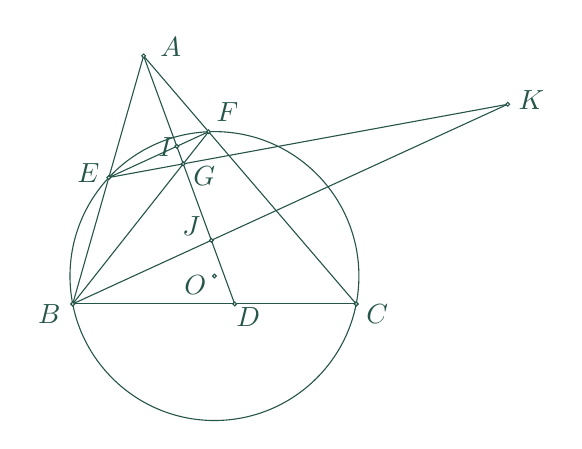
\begin{tikzpicture}[scale=0.45,thachthuctoanhoc]
			\draw [] (0.,6.)-- (-2.,-1.);
			\draw [] (-2.,-1.)-- (6.,-1.);
			\draw [] (6.,-1.)-- (0.,6.);
			\draw [] (0.,6.)-- (2.571428571428571,-1.);
			\draw [] (2.,-0.21319850709788402) circle (4.0766477146342925cm);
			\draw [] (-2.,-1.)-- (1.8342197011320263,3.86007701534597);
			\draw [] (-0.9805577018630328,2.5680480434793846)-- (1.8342197011320263,3.86007701534597);
			\draw [] (-0.9805577018630328,2.5680480434793846)-- (10.276729559748448,4.635220125786173);
			\draw [] (-2.,-1.)-- (10.276729559748448,4.635220125786173);
			\draw (0.19834439641082918,6.781346828913015) node[anchor=north west] {$A$};
			\draw (-3.25581020883794574,-0.7341839715584899) node[anchor=north west] {$B$};
			\draw (6.008413230363799,-0.7540138681296548) node[anchor=north west] {$C$};
			\draw (2.339882364698284,-0.8333334544143145) node[anchor=north west] {$D$};
			\draw (-2.1467773632500454,3.231795342674494) node[anchor=north west] {$E$};
			\draw (1.7846452607056653,4.9717999227203) node[anchor=north west] {$F$};
			\draw (1.1302586738572222,3.1455135816824) node[anchor=north west] {$G$};
			\draw (0.146813630069335,3.978829638112873) node[anchor=north west] {$I$};
			\draw (0.87196812138191,0.07884178785927186) node[anchor=north west] {$O$};
			\draw (0.82174327112016,1.74448581273216) node[anchor=north west] {$J$};
			\draw (10.311500786306592,5.294104586075646) node[anchor=north west] {$K$};
			\draw [fill=white] (0.,6.) circle (1.5pt);
			\draw [fill=white] (-2.,-1.) circle (1.5pt);
			\draw [fill=white] (6.,-1.) circle (1.5pt);
			\draw [fill=white] (2.571428571428571,-1.) circle (1.5pt);
			\draw [fill=white] (2.,-0.21319850709788402) circle (1.5pt);
			\draw [fill=white] (-0.9805577018630328,2.5680480434793846) circle (1.5pt);
			\draw [fill=white] (-2.,-1.) circle (1.5pt);
			\draw [fill=white] (6.,-1.) circle (1.5pt);
			\draw [fill=white] (1.8342197011320263,3.86007701534597) circle (1.5pt);
			\draw [fill=white] (1.1190840291604753,2.9536045872853722) circle (1.5pt);
			\draw [fill=white] (0.9373267009792919,3.448388425111928) circle (1.5pt);
			\draw [fill=white] (1.9118236472945893,0.7955911823647293) circle (1.5pt);
			\draw [fill=white] (10.276729559748448,4.635220125786173) circle (1.5pt);
		\end{tikzpicture}
		\vspace*{-10pt}
	\end{figure}
	Do bốn điểm $B$, $C$, $E$, $F$ cùng thuộc một đường tròn, nên
	\begin{align*}
		\left( {EF;AB} \right) &\equiv \left( {EF;EB} \right) \equiv \left( {CF;CB} \right) \\
		&\equiv \left( {CA;CB} \right)\;\;\;\left( {{\rm{mod}}\;\pi } \right).
	\end{align*}
	Suy ra, đường thẳng $EF$ có phương không đổi.                    \hfill ($1$)
	\vskip 0.05cm
	Gọi $I$ là giao điểm của $AD$ và $EF$. Do ($1$) nên theo định lý Thales, tỷ số $\dfrac{{\overline {IE} }}{{\overline {IF} }}$ là một hằng số, khi $E$, $F$ thay đổi.                                                               \hfill ($2$)
	\vskip 0.05cm
	Qua $B$, kẻ đường thẳng song song với $EF$, cắt $AD$, $EG$ tại $J$, $K$, tương ứng.
	\vskip 0.05cm
	Do $B$ là điểm cố định nên từ $BK \parallel EF$ và ($1$) suy ra, $BK$ là đường thẳng cố định. Vì thế, giao điểm $J$ của $BK$ và đường thẳng cố định $AD$ là một điểm cố định.
	\vskip 0.05cm
	Do $BK \parallel EF$ nên theo định lý Thales, ta có:
	\begin{align*}
		\frac{{\overline {JB} }}{{\overline {JK} }} = \frac{{\overline {IE} }}{{\overline {IF} }}
	\end{align*}
	Kết hợp với ($2$) suy ra, $\dfrac{{\overline {JB} }}{{\overline {JK} }}$ là một hằng số; mà $B$ và $J$ là các điểm cố định, nên $K$ là một điểm cố định.
	\vskip 0.05cm
	Vì vậy, $GE$ luôn đi qua một điểm cố định. Ta có điều phải chứng minh theo yêu cầu đề bài.
	\vskip 0.05cm
	\textbf{\color{thachthuctoanhoc}Bình luận và Nhận xét}
	\vskip 0.05cm
	$\pmb{1.}$ Ở Lời giải trên, ta đã chứng minh kết luận của bài ra với giả thiết nhẹ nhàng hơn: Đường tròn $(O)$ thay đổi, đi qua $B$, $C$, và cắt các \textit{đường thẳng} $AB$, $AC$ tương ứng tại $E$, $F$, khác $A$, $B$, $C$.
	\vskip 0.05cm
	$\pmb{2.}$ Đường thẳng $EF$ trong bài toán được gọi là \textit{đường đối song của $BC$ đối với tam giác $ABC$}. Các kết quả về đường đối song đã được trình bày trong nhiều tài liệu về Hình học sơ~cấp.
	\vskip 0.05cm
	$\pmb{3.}$ Rất tiếc, trong các lời giải Tạp chí đã nhận được từ bạn đọc, có một lời giải sai, do người giải bài đã \textit{khẳng định sai} rằng, đường thẳng $EF$ song song với đường thẳng đi qua chân hai đường cao, kẻ từ $B$, $C$ của tam\linebreak giác $ABC$.
	\vskip 0.05cm
	\textbf{\color{thachthuctoanhoc}\textit{Lưu ý rằng}}, hai đường thẳng nêu trên có thể trùng nhau; và trong trường hợp tam giác $ABC$ vuông ở $A$, đường thẳng thứ hai hoàn toàn không xác định!
	\vskip 0.2cm
	\hfill	\textbf{\color{thachthuctoanhoc}Hạ Vũ Anh}
	\vskip 0.2cm
	{\color{thachthuctoanhoc}{\usefont{T5}{qag}{b}{n} P650.}}
	(Mức $A$)
	Cho $p$ là một số nguyên tố có dạng $4k + 3$, $k \in \mathbb{N}$. Xét dãy số Fibonacci $(F_n)$, xác định bởi: $F_0 = 0, F_1 = 1$,    và
	\begin{align*}
		{F_{n + 2}} = {F_{n + 1}} + {F_n}	\text{ với mọi } n \ge 0.
	\end{align*}
	Chứng minh rằng, không tồn tại các số nguyên dương $m, n$, với $n \ge 5$, sao cho \linebreak $F_n = p^m$.
	\vskip 0.05cm
	\textbf{\color{thachthuctoanhoc}Lời giải} (\textit{dựa theo lời giải của bạn Trần Minh Hoàng, lớp $10$T$1$, trường THPT chuyên Hà Tĩnh, tỉnh Hà Tĩnh})\textbf{\color{thachthuctoanhoc}.}
	\vskip 0.05cm
	Trước hết, ta nhắc lại (không chứng minh) hai tính chất đơn giản sau, của dãy Fibonacci:
	\vskip 0.05cm
	$1/$ Với mọi  $k \in \mathbb{N^*}$, $F_k^2 + F_{k + 1}^2 = {F_{2k + 1}}.$
	\vskip 0.05cm
	$2/$ Với mọi $k, m \in \mathbb{N^*}$, ${F_m}\mid{F_{km}}.$
	\vskip 0.05cm
	\textit{Trở lại bài toán.}
	\vskip 0.05cm
	Giả sử ngược lại, tồn tại các số nguyên dương $m, n$, với $n \ge 5$, sao cho  $F_n = p^m$. \hfill ($*$)
	\vskip 0.05cm
	Do $F_6 = 8$, không là lũy thừa của một số nguyên tố có dạng $4k + 3$, nên $n \ne 6$.
	\vskip 0.05cm
	Xét các trường hợp sau:
	\vskip 0.05cm
	$\diamond$ \textit{Trường hợp} $1$: $n$ là số lẻ lớn hơn $3$.
	\vskip 0.05cm
	Đặt $n = 2h + 1$, $h \ge 2$; theo $1/$, ta có:
	\begin{align*}
		{F_n} = {F_{2h + 1}} = F_h^2 + F_{h + 1}^2.
	\end{align*}
	Kết hợp với ($*$), suy ra
	\begin{align*}
		p\mid F_h^2 + F_{h + 1}^2.
	\end{align*}
	Mà $p$ là số nguyên tố có dạng $4k + 3$, nên $p\mid {F_h}$ và $p\mid {F_{h + 1}}$.  Do đó
	\begin{align*}
		p\mid{F_{h + 1}} - {F_h} = {F_{h - 1}}.
	\end{align*}
	Vì thế
	\begin{align*}
		p\mid{F_h} - {F_{h - 1}} = {F_{h - 2}}.
	\end{align*}
	Tiếp tục quá trình suy luận như trên, ta được $p\mid{F_1} = 1,$  là điều vô lý. Vì vậy, $n$ phải là số chẵn.
	\vskip 0.05cm
	$\diamond$ \textit{Trường hợp} $2$: $n$ là số chẵn, có ước lẻ $t > 3$.
	\vskip 0.05cm
	Do $t \mid n $  nên theo $2/$, ta có
	\begin{align*}
		{F_t}\mid{F_n} = {p^m}. 
	\end{align*}
	Suy ra, tồn tại số nguyên dương $s$, sao cho ${F_t} = {p^s},$ là điều vô lý (theo kết quả xét trường hợp $1$). Vì vậy, với lưu ý $n \ne 6$, suy ra phải xảy ra:
	\vskip 0.05cm
	$\diamond$ \textit{Trường hợp} $3$: $n$ có dạng $n = {2^s},$ với $s \in \mathbb{N^*}$ và $s \ge 3$.
	\vskip 0.05cm
	Do $s \ge 3$ nên  ${2^3} = 8\mid{2^s}$. Do đó, theo $2/$, ta có
	\begin{align*}
		{F_8} = 21\mid{F_{{2^s}}} = {F_n} = {p^m},
	\end{align*}
	là điều vô lý. Điều vô lý này cho thấy, giả sử ($*$) là sai. Vì thế, ta có điều phải chứng minh theo yêu cầu đề bài.
	\vskip 0.05cm
	\textbf{\color{thachthuctoanhoc}Bình luận và Nhận xét}
	\vskip 0.05cm
	$\pmb{1.}$ Bạn đọc có thể chứng minh tính chất $1/$ (nêu trong Lời giải trên) bằng cách sử dụng công thức số hạng tổng quát của dãy Fibonacci, và chứng minh tính chất $2/$ bằng phương pháp quy nạp theo $k$.
	\vskip 0.05cm
	$\pmb{2.}$ Trong Lời giải trên, ta đã sử dụng (không chứng minh) kết quả sau:
	\vskip 0.05cm
	“\textit{Với $a, b$ là các số nguyên, và $p$ là số nguyên tố có dạng $4k + 3$, nếu $p\mid{a^2} + {b^2}$  thì  $p \mid a$ và  $p \mid b$}”
	\vskip 0.05cm
	Sử dụng định lý nhỏ Fermat, bạn đọc có thể dễ dàng chứng minh kết quả trên bằng phương pháp phản chứng.
	\vskip 0.05cm
	$\pmb{3.}$ Trong bài báo “Classical and
	modular approaches to exponential Diophantine equations I. Fibonacci and Lucas perfect powers”, đăng tải trong Annals of Mathematics, $163$ ($2006$) (trang $969 - 1018$), các nhà toán học Yann Bugeaud, Maurice Mignotte và Samir Siksek đã chứng minh được rằng, \textit{trong dãy Fibonacci, \textbf{\color{thachthuctoanhoc}chỉ có} các số hạng $F_0=0, F_1 = 1, F_2 = 1, F_6 = 8$ và $F_{12} = 144$ là các lũy thừa hoàn hảo của một số nguyên.}
	\vskip 0.05cm
	$\pmb{4.}$ Tất cả các lời giải Tạp chí đã nhận được từ bạn đọc đều là lời giải đúng và hoàn chỉnh.
	\begin{flushright}
		\textbf{\color{thachthuctoanhoc}Lưu Thị Thanh Hà}
	\end{flushright}
\end{multicols}
\centerline{\textbf{\color{thachthuctoanhoc}DANH SÁCH HỌC SINH CÓ LỜI GIẢI HOÀN CHỈNH}}
\vskip 0.1cm
\textit{Trong các ngoặc đơn ở phần dưới đây, sau tên lớp là mã hiệu của các bài toán mà học sinh có lời giải hoàn chỉnh.}
\begin{multicols}{2}
	\textbf{\color{thachthuctoanhoc}KHỐI THCS}
	\vskip 0.1cm
	$\bullet$ Trường \textbf{\color{thachthuctoanhoc}THCS xã Pom Lót}, huyện Điện Biên, tỉnh Điện Biên: \textit{Nguyễn Ngọc Diệp} (lớp $9$D$3$; P$641$).
	\vskip 0.1cm
	$\bullet$ Trường \textbf{\color{thachthuctoanhoc}THPT chuyên Hà Nội -- Amsterdam}, Tp. Hà Nội: \textit{Trần Hữu Đức Hiếu} (lớp $8$A; P$641$, P$644$, P$645$).
	\vskip 0.1cm
	$\bullet$ Trường \textbf{\color{thachthuctoanhoc}THCS Lê Quý Đôn}, Quận $3$, Tp. Hồ Chí Minh: \textit{Nguyễn Trịnh Phương Minh} (lớp $6/14$; P$641$), \textit{Nguyễn Chánh Thiện} (lớp $8/14$; P$641$).
	\vskip 0.1cm
	$\bullet$ Trường \textbf{\color{thachthuctoanhoc}THCS Phúc Yên}, Tp. Phúc Yên, tỉnh Vĩnh Phúc: \textit{Vũ Bảo Lân} (lớp $8$A$5$; P$644$).
	\vskip 0.2cm
	\textbf{\color{thachthuctoanhoc}KHỐI THPT}
	\vskip 0.2cm
	$\bullet$ Trường \textbf{\color{thachthuctoanhoc}THPT chuyên Lý Tự Trọng}, Tp. Cần Thơ: \textit{Đàm Lương Gia An} (lớp $11$A$1$B; P$650$).
	\vskip 0.1cm
	$\bullet$ Trường \textbf{\color{thachthuctoanhoc}THPT chuyên Nguyễn Quang Diêu}, tỉnh Đồng Tháp: \textit{Nguyễn Hải Đăng} (lớp $12$T$1$; P$641$),  \textit{Lư Gia Hưng} (lớp $11$T$1$; P$641$, P$645$), \textit{Huỳnh Ngọc Ngân} (lớp $11$T$1$; P$645$), \textit{Đỗ Duy Quang} (lớp $11$T$1$; P$641$, P$645$).
	\vskip 0.1cm
	$\bullet$ Trường \textbf{\color{thachthuctoanhoc}THPT chuyên Hà Nội -- Amsterdam}, Tp. Hà Nội: \textit{Phạm Đăng Minh} (lớp $10$ Toán $2$; P$650$).
	\vskip 0.1cm
	$\bullet$ Trường \textbf{\color{thachthuctoanhoc}THPT chuyên Hà Tĩnh}, tỉnh Hà Tĩnh: \textit{Trần Minh Hoàng} (lớp $10$T$1$; P$647$, P$648$, P$649$, P$650$).
	\vskip 0.1cm
	$\bullet$ Trường \textbf{\color{thachthuctoanhoc}THPT chuyên Hưng Yên}, tỉnh Hưng Yên: \textit{Trần Hữu Dương} (lớp $11$ Toán $1$; P$641$, P$645$), \textit{Nguyễn Gia Khánh} (lớp $11$ Toán $1$; P$648$, P$649$).
	\vskip 0.1cm
	$\bullet$ Trường \textbf{\color{thachthuctoanhoc}THPT chuyên Lê Hồng Phong}, tỉnh Nam Định: \textit{Nguyễn Đức Khải} (lớp $11$ Toán $2$; P$645$), \textit{Bùi Khánh Linh} (lớp $10$ Toán $2$; P$641$, P$645$).
	\vskip 0.1cm
	$\bullet$ Trường \textbf{\color{thachthuctoanhoc}THPT chuyên Lương Văn Chánh}, tỉnh Phú Yên: \textit{Nguyễn Thị Bảo Tiên} (lớp $11$ Toán $1$; P$645$).
	\vskip 0.1cm
	$\bullet$ Trường \textbf{\color{thachthuctoanhoc}THPT chuyên Nguyễn Bỉnh Khiêm}, tỉnh Quảng Nam: \textit{Trịnh Quốc Khánh} (lớp $11/1$; P$649$).
	\vskip 0.1cm
	$\bullet$ Trường \textbf{\color{thachthuctoanhoc}THPT chuyên Tiền Giang}, tỉnh Tiền Giang: \textit{Phan Tiến Đạt} (lớp $10$ Toán; P$644$), \textit{Nguyễn Huy Hoàng} (lớp $10$ Toán; P$641$), \textit{Lê Gia Khiết} (lớp $10$ Toán; P$644$), \textit{Trần Phúc Thịnh} (lớp $10$ Toán; P$641$).
	\vskip 0.1cm
	$\bullet$ Trường \textit{THPT chuyên Quốc học Huế}, tỉnh Thừa Thiên -- Huế: \textit{Nguyễn Thị Nhật Thảo} (lớp $11$ Toán $2$; P$641$), \textit{Trần Thị Thanh Thư} (lớp $12$ Toán $1$; P$641$), \textit{Đặng Quỳnh Bảo Uyên} (lớp $11$ Toán $2$; P$641$).
	\vskip 0.1cm
	$\bullet$ Trường \textit{THPT chuyên Khoa học tự nhiên}, ĐH Khoa học tự nhiên -- ĐHQG Hà Nội: \textit{Vương Khánh Toàn} (lớp $10$A$1$ Toán; P$641$, P$642$, P$644$, P$645$).
	\vskip 0.1cm
	$\bullet$ Trường \textbf{\color{thachthuctoanhoc}THPT chuyên Sư phạm}, ĐH Sư phạm Hà Nội: \textit{Hồ Trần Khánh Linh} (lớp $12$ Toán $2$; P$649$).
\end{multicols}



	\newpage 
	
	\setcounter{figure}{0}
	\thispagestyle{hoccungpinone}
\pagestyle{hoccungpi}
\everymath{\color{hoccungpi}}
\graphicspath{{../hoccungpi/pic/}}
\blfootnote{$^{1}$\color{hoccungpi}Đại học Bách Khoa Hà Nội.}
\begingroup
\AddToShipoutPicture*{\put(0,616){\includegraphics[width=19.3cm]{../bannerhoccungpi}}}
\AddToShipoutPicture*{\put(116,525){\includegraphics[scale=1]{../tieude.pdf}}}
\centering
\endgroup
\vspace*{185pt}

\begin{multicols}{2}
	Dãy số Fibonacci, đặt theo tên nhà toán học người Ý Fibonacci ($1170-1250$), được xác định bởi $F_0=0$, $F_1=1$, $F_{n+1}=F_n+F_{n-1}$ với mọi $n\geq 1$. 
	Đây là một trong những dãy số nổi tiếng nhất trong toán học. Tạp chí toán học Fibonacci Quaterly [$3$] của Canada chỉ xuất bản những nghiên cứu liên quan đến dãy Fibonacci. Vào năm $1964$, nhà toán học người Anh John H. E. Cohen chứng minh  có đúng ba số chính phương trong dãy Fibonacci, đó là $0$, $1$, và $144$ [$2$]. Một câu hỏi tự nhiên là liệu ta có thể tìm tất cả các giai thừa trong dãy Fibonacci. Câu hỏi này được giải quyết bởi Rajagopal và Griffiths [$5$]. Họ chỉ ra $1!$ và $2!$ là  hai số giai thừa duy nhất trong dãy Fibonacci. Nói cách khác, ta có định lý sau.
	\vskip 0.1cm
	\textbf{\color{hoccungpi}Định lý} $\pmb{1.}$ \textit{Phương trình
		\begin{align*}
			F_n=m! \tag{$1$}
		\end{align*}
		không có nghiệm nguyên dương với $n\ge 4$, trong đó $F_n$ là số Fibonacci thứ $n$. }
	\vskip 0.1cm
	Tuy nhiên, chứng minh của Rajagopal và Griffiths sử dụng định lý Carmichael về ước số nguyên thủy [$1$], một kết quả không tầm thường. Trong bài báo này, tác giả trình bày một chứng minh khác cho Định lý $1$. Với mỗi số nguyên dương $m$, ta ký hiệu $v_2(m)$ là số mũ cao nhất của $2$ chia hết $m$. Chú ý rằng với mọi $n > 0$ thì
	\begin{align*}
		F_n=\dfrac{u^n-v^n}{u-v}> \dfrac{u^n-1}{\sqrt{5}},
	\end{align*}
	trong đó $u=(1+\sqrt{5})/2$ và $v=(1-\sqrt{5})/2$.
	\vskip 0.1cm	
	Ta cần một số bổ đề.
	\vskip 0.1cm
	\textbf{\color{hoccungpi}Bổ đề} $\pmb{2}.$
	\textit{Với mọi số nguyên dương $n$ thì}
		\begin{align*}
			v_2(F_n)=
			\begin{cases}
				0 \text{ nếu } n\not\equiv 0 \,\,(\!\bmod{3})\\
				1 \text{ nếu } n\equiv 3 \,\,(\!\bmod{6}) \quad\quad\quad\text{\color{black}(}2\text{\color{black})}\\ 
				v_2(n)+2 \text{ nếu } n \equiv 0 \,\,(\!\bmod{6}).
			\end{cases} 
		\end{align*}
	Trong chứng minh Bổ đề [$2$], ta cần đến dãy số Lucas. Dãy Lucas $(L_n)_{n\geq 0}$ được xác định bởi  $L_0=2,\, L_1=1,\, L_{n+1}=L_n+L_{n-1}$ với mọi $n\geq 1$. Chú ý rằng $L_n=u^n+v^n$ với mọi $n\geq 0$.
	\vskip 0.1cm
	\textit{Chứng minh.} Xét dãy $(F_n)_{n\geq 0}$ modulo $4$: $0$, $1$, $1$, $2$, $3$, $1$, $0$, $1$, $1$, $2$, $3$, $...$ Đây là một dãy tuần hoàn theo chu kỳ $6$. Dễ thấy ($2$) đúng với $n\leq 6$. Giả sử ($2$) đúng với $n<k$ ($k\geq 6$, $k\in \mathbb{Z}^{+}$). Xét $n=k$. 
	Ta chỉ cần xét trường hợp $6\mid k$ vì nếu không $v_2(F_k)=0$ khi $3\nmid k$ và $v_2(F_k)=1$ khi $6\mid (k-3)$.
	\vskip 0.1cm	
	Đặt $k=6m$, với $m\in \mathbb{Z}^{+}$. Khi đó 
	\begin{align*}
			F_n&=\dfrac{u^{6m}-v^{6m}}{u-v}=\dfrac{u^{3m}-v^{3m}}{u-v}(u^{3m}+v^{3m})\\
			&=F_{3m}L_{3m}. \tag{$3$}
	\end{align*}
	Xét dãy $(L_n)_{n\geq 0}$  modulo $8$, dãy này có dạng:
		$2$, $1$, $3$, $4$, $7$, $3$, $2$, $5$, $7$, $4$, $3$, $7$, $2$, $1$, $3$, $...$
		Từ đó suy ra dãy Lucas modulo $8$ tuần hoàn với chu kỳ $12$. Hơn nữa, $8\nmid L_n$ với mọi $n\in \mathbb{Z}^{+}$ và 
		\begin{align*}
			v_2(L_n)=\begin{cases}
				0 \text{ nếu } n\equiv 1,2 \,\,(\!\bmod{3})\\
				2 \text{ nếu } n\equiv 3 \,\,(\!\bmod{6}) \quad\quad\quad \text{\color{black}(}4\text{\color{black})}\\ 
				1 \text{ nếu } n\equiv 0 \,\,(\!\bmod{6}).
			\end{cases} 
		\end{align*}
		Nếu $2\nmid m$ thì $3m\equiv 3 \pmod {6}$. Theo ($4$) thì $v_2(L_{3m})=2$. Từ ($3$) suy ra
		\begin{align*}
			v_2(F_{6m})=v_2(F_{3m})+2=3.
		\end{align*}
		Nếu $2|m$ thì $3m\equiv 0 \pmod {6}$. Theo ($4$)
		thì $v_2(L_{6m})=1$. Từ ($4$) suy ra
		\begin{align*}
			v_2(F_{6m})=v_2(F_{3m})+1=v_2(m)+3.
		\end{align*}
		Suy ra ($2$) đúng với $n=k+1$. Bổ đề được chứng minh. \hfill $\square$
	\vskip 0.1cm
	\textbf{\color{hoccungpi}Bổ đề} $\pmb{3.}$ \textit{Với mọi số nguyên dương {$n$} thì} 
		\begin{align*}
			v_2(n!)\geq n-1-\log_2 n.\tag{$5$}
		\end{align*}
	\textit{Chứng minh.}
	Giả sử $n$ có biểu diễn theo hệ nhị phân là
	\begin{align*}
		\overline{{s_ks_{k-1}}\ldots s_1}_{(2)}=n.
	\end{align*}
	Khi đó $s_k=1$ và $n\geq 2^{k-1}$.
	Đặt $S_2(n)=s_1+s_2+\cdots+s_k$.
	Thì
	\begin{align*}
		S_2(n)\leq k \leq 1+ \log_2 n.
	\end{align*}
	Mặt khác theo công thức Legendre\footnote[2]{\color{hoccungpi}Công thức Legendre nói rằng với mọi số nguyên tố $p$ thì $v_p(n!)=(n-S_p(n))/(p-1)$, trong đó $S_p(n)$ là tổng các chữ số trong biểu diễn cơ số $p$ của $n$.}   thì
	\begin{align*}
		v_2(n!)=n-S_2(n).
	\end{align*}
	Nên 
	\begin{align*}
	\quad\quad\quad	v_2(n!)\geq n-1-\log_2 n. \,\,\,\,\quad\quad\quad \square
	\end{align*}
	\textbf{\color{hoccungpi}Bổ đề} $\pmb{4.}$
	\textit{Với mọi số nguyên dương $n\geq 15$ thì}
		\begin{align*}
			2^{n-3}>n^3. \tag{$6$}
		\end{align*}
	\textit{Chứng minh.}
		Với $n=15$ thì ($6$) đúng vì $2^{12}=4096>3375=15^3$. Giả sử ($6$) đúng với $n=m\geq 15$. Khi đó 
		\begin{align*}
			2^{m+1-3} &=2\cdot 2^{m-3}>2m^3=m^3+m^3\\
			&\ge m^3+ 15m^2 = m^3 +\! 3m^2 \!+\! 3m +\! 1\\
			&\quad +3 (m^2-m)+ (m^2-1)+ 8m^2 \\
			&> m^3+3m^2+3m+1=(m+1)^3.
		\end{align*}
		Suy ra ($6$) đúng với $n=m+1$. Theo quy nạp có ($6$) đúng với mọi $n\geq 15$. \hfill $\square$
	\vskip 0.1cm
	\textbf{\color{hoccungpi}Bổ đề} $\pmb{5.}$
	\textit{Với mọi số nguyên dương $n\geq 2$ thì 
		\begin{align*}
			u^{n^2}>1+\sqrt{5}n!, \tag{$7$}
		\end{align*}
		trong đó $u=(1+\sqrt{5})/2$. }
	\vskip 0.1cm
	\textit{Chứng minh.} 
	Với $n=2$ thì ($7$) trở thành $u^4> 1+ 2\sqrt{5}$, hay $\frac{7+3\sqrt{5}}{2}> 1+ 2\sqrt{5}$, hay, một cách tương đương, $5> \sqrt{5}$, do đó hiển nhiên đúng. 
	\vskip 0.1cm	
	Giả sử ($7$) đúng với $n=m\geq 2$. Trước hết, để ý rằng $u^2 = \frac{3+ \sqrt{5}}{2}>2$, nói riêng $u^{2m}> 2^m= (1+1)^m = 1+ \binom{m}{1} + \cdots > m+1$ với mọi $m\ge 2$. Từ đó,
	\begin{align*}
			u^{(m+1)^2}&=u^{m^2}\cdot u^{2m+1}\\
			&> u^{m^2}\cdot u^{2m}\\
			&>(1+\sqrt{5}m!)(m+1)\\
			&>1+\sqrt{5}(m+1)!.
	\end{align*}
	Suy ra ($7$) đúng với $n=m+1$. Như vậy, theo nguyên lý quy nạp thì ($7$) đúng với mọi \linebreak $n\geq 2$.\hfill $\square$
	\vskip 0.1cm
	Bây giờ ta chứng minh Định lý $1$.
	\vskip 0.1cm
	\textit{Chứng minh.}
	Giả sử tồn tại các số nguyên dương $m,n$ với $n\geq 4$ sao cho
	\begin{align*}
			F_n=m!. \tag{$8$}
	\end{align*}
	Do $F_4=3$ không là một số giai thừa nên ta phải có $F_n\geq F_5 =5$, dẫn đến $m\geq 3$. Nếu $m=4$ thì $F_n=24$, điều này là vô lý do dãy Fibonacci là dãy số tăng kể từ số hạng thứ ba và $F_8=21< 24< F_9=34$. Suy ra $m\geq 5$. Khi đó $3,4,5$ đều là ước của $m!$ nên cũng là ước của $F_n$. Theo ($2$) ta có $6\mid n$. 
	\vskip 0.1cm	
	Xét dãy $(F_n)_{n\geq 0}$  modulo $3$: $0$, $1$, $1$, $2$, $0$, $2$, $2$, $1$, $0$, $1$, $1$, $...$ Từ đó suy ra dãy Fobonacci modulo $3$ tuần hoàn với chu kỳ $8$ và $3\mid F_n$ khi và chỉ khi $4\mid n$.
	\vskip 0.1cm
	Xét dãy $(F_n)_{n\geq 0}$ modulo $5$:
	$0$, $1$, $1$, $2$, $3$, $0$, $3$, $3$, $1$, $4$, $0$, $4$, $4$, $3$, $2$, $0$, $2$, $2$, $4$, $1$, $0$, $1$, $1$, $...$
	Suy ra dãy Fibonacci modulo $5$ tuần hoàn với chu kỳ $20$ và $5\mid F_n$ khi và chỉ khi $5\mid n$. 
	\vskip 0.1cm	
	Từ các lập luận trên ta suy ra $4,5,6$ đều là ước của $n$. Suy ra $60\mid n$. Nói riêng, ta có $n\geq 60$. Chú ý rằng $u^2>2$ nên
	\begin{align*}
		m!=F_n\geq F_{60}>\dfrac{u^{60}-1}{\sqrt{5}}>15!.
	\end{align*}
	Trong ước lượng trên, bất đẳng thức $(u^{60}-1)/(15!\sqrt{5})>1$ có thể được kiểm tra bằng các tính toán trực tiếp dựa vào các phần mềm tính toán hoặc chỉ đơn giản bằng một chiếc máy tính cầm tay.
	Suy ra 
	\begin{align*}
		m\geq 16.
	\end{align*} 
	Nhắc lại rằng, theo ($2$) thì
	\begin{align*}
		v_2(F_n)=2+v_2(n).
	\end{align*}
	Kết hợp điều này với ($5$) ta suy ra 
	\begin{align*}
		2+v_2(n)= v_2(m!)\geq m-1-\log_2 m,
	\end{align*}
	cho nên 
	\begin{align*}
		v_2(n)\geq m-3-\log_2 m.
	\end{align*}
	Do đó, ta có 
	\begin{align*}
			n\geq 2^{v_2(n)}\geq  \dfrac{2^{m-3}}{m}. \tag{$9$}
	\end{align*}
	Chú ý rằng $m\geq 16$ nên bằng cách kết hợp ($6$), ($7$), và ($9$) ta thu được
	\begin{align*}
		m!=F_n&>\dfrac{u^n-1}{\sqrt{5}}>\dfrac{u^{2^{m-3}/{m}}-1}{\sqrt{5}}\\&>\dfrac{u^{m^2}-1}{\sqrt{5}}>m!,
	\end{align*}
	vô lý. Định lý $1$ được chứng minh. \hfill $\square$
	\vskip 0.1cm
	\textbf{\color{hoccungpi}Tài liệu tham khảo}
	\vskip 0.1cm
	[$1$] R. D. Carmichael, On the numerical factors of the arithmetic forms $\alpha^n\pm \beta^n$, Annals of Mathematics, $15$ ($1/4$) ($1913$), $30-70$.
	\vskip 0.1cm
	[$2$] J. H. E. Cohn, Square Fibonacci numbers, Fibonacci Quarterly, $2$ ($2$)
		($1964$), $109-113$.
	\vskip 0.1cm
	[$3$] Fibonacci Quaterly. \url{https://www.fq.math.ca/}
	\vskip 0.1cm
	[$4$] Legendre's formula, Wikipedia. \url{https://en.wikipedia.org/wiki/Legendre%27s_formula}
	\vskip 0.1cm
	[$5$] S.~Rajagopal và M.~Griffiths,  On Fibonacci numbers that are factorials, Mathematical Gazette, {$98$} ($541$) (March $2014$), $104-107$.
\end{multicols}
	\newpage
	
	\setcounter{figure}{0}
	\thispagestyle{cackithitoannone}
\pagestyle{cackithitoan}
\everymath{\color{cackithi}}
\graphicspath{{../cackithi/pic/}}
\begingroup
\AddToShipoutPicture*{\put(0,616){\includegraphics[width=19.3cm]{../bannercackithi}}} 
\AddToShipoutPicture*{\put(150,575){\includegraphics[scale=1]{../tieude1.pdf}}}
\centering
\endgroup
\vspace*{130pt}

\begin{multicols}{2}
	Trong phần đầu chuyên mục, chúng tôi sẽ trình bày lời giải của các bài toán trong kỳ thi Olympic Toán học Trẻ của Estonia năm học $2020-2021$, đăng trong số báo $10/2022$. 
	\vskip 0.1cm
	{\bf\color{cackithi} OC$\pmb{22.}$} Tia phân giác tại đỉnh $A$ của tam giác $ABC$ cắt đường tròn ngoại tiếp tam giác $ABC$ tại điểm $F (F \neq A).$ Lấy điểm $D$ và $E$ lần lượt trên các cạnh $AB$ và $AC$ sao cho $DE$ song song với $BC$. Gọi $G$ và $H$ lần lượt là giao điểm của các tia $FD$ và $FE$ với đường tròn ngoại tiếp tam giác $ABC (G \neq F, H \neq F).$ Các đường tròn ngoại tiếp tam giác $AGD$ và $AHE$ cắt nhau tại điểm $P (P \neq A).$ Chứng minh rằng điểm $P$ nằm trên đường thẳng $AF.$
	\begin{figure}[H]
		\vspace*{-10pt}
		\centering
		\captionsetup{labelformat= empty, justification=centering}
		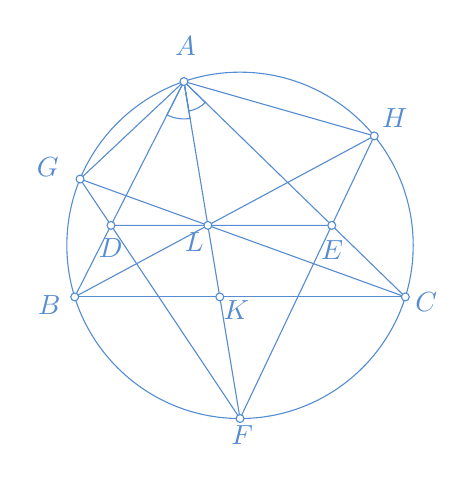
\begin{tikzpicture}[cackithi,scale=0.95, node font=/small]
			\draw [shift={(3.46,2.88)}] (0,0) -- (-80.54882573391929:0.4) arc (-80.54882573391929:-44.21517539700811:0.4) -- cycle;
			\draw [shift={(3.46,2.88)}] (0,0) -- (-116.88247607083048:0.5) arc (-116.88247607083048:-80.54882573391929:0.5) -- cycle;
			\draw  (3.46,2.88)-- (2.,0.);
			\draw  (2.,0.)-- (6.42,0.);
			\draw  (3.46,2.88)-- (6.42,0.);
			\draw  (4.21,0.6897222222222221) circle (2.315127802914379cm);
			\draw  (3.46,2.88)-- (4.21,-1.6254055806921568);
			\draw  (2.485169230769231,0.9570461538461539)-- (5.436547750464446,0.9568724590075657);
			\draw  (2.0714369973952342,1.576494474673352)-- (4.21,-1.6254055806921568);
			\draw  (4.21,-1.6254055806921568)-- (6.0044579560443,2.1525063443046544);
			\draw  (2.0714369973952342,1.576494474673352)-- (3.46,2.88);
			\draw  (3.46,2.88)-- (6.0044579560443,2.1525063443046544);
			\draw  (2.0714369973952342,1.576494474673352)-- (6.42,0.);
			\draw  (2.,0.)-- (6.0044579560443,2.1525063443046544);
			\draw [fill=white] (3.46,2.88) circle (1.5pt);
			\draw (3.48,3.35) node {$A$};
			\draw [fill=white] (2.,0.) circle (1.5pt);
			\draw (1.66,-0.11) node {$B$};
			\draw [fill=white] (6.42,0.) circle (1.5pt);
			\draw (6.7,-0.07) node {$C$};
			\draw [fill=white] (4.21,-1.6254055806921568) circle (1.5pt);
			\draw (4.24,-1.85) node {$F$};
			\draw [fill=white] (2.485169230769231,0.9570461538461539) circle (1.5pt);
			\draw (2.48,0.65) node {$D$};
			\draw [fill=white] (5.436547750464446,0.9568724590075657) circle (1.5pt);
			\draw (5.44,0.63) node {$E$};
			\draw [fill=white] (2.0714369973952342,1.576494474673352) circle (1.5pt);
			\draw (1.64,1.73) node {$G$};
			\draw [fill=white] (6.0044579560443,2.1525063443046544) circle (1.5pt);
			\draw (6.28,2.39) node {$H$};
			\draw [fill=white] (3.7800041573402137,0.9569699500850757) circle (1.5pt);
			\draw (3.6,0.73) node {$L$};
			\draw [fill=white] (3.939424096524548,0.) circle (1.5pt);
			\draw (4.16,-0.17) node {$K$};
		\end{tikzpicture}
		\vspace*{-10pt}
	\end{figure}
	\textit{Lời giải.} 
	Ta gọi $K, L$ lần lượt là giao điểm của $AF$ với $BC, DE.$
	Theo giả thiết $AF$ là phân giác của góc $\angle BAC$ nên ta có:
	\begin{align*}
		\angle AHF&=\angle ACB \!+\! \angle BCF\\
		&= \angle ACK \!+\! \angle KAC \!=\! 180^\circ \!-\!\angle AKC.
	\end{align*}   
	Mặt khác do $DE$ song song với $BC$ nên $\angle ALE = \angle AKC.$ Từ đó ta suy ra $\angle AHF$ và $\angle ALE$ là bù nhau, tức là tứ giác $AHEL$ nội tiếp.
	\vskip 0.1cm
	Chứng minh tương tự ta cũng có tứ giác $AGDL$ nội tiếp. Như vậy đường tròn ngoại tiếp hai tam giác $AGD$ và $AHE$ cùng đi qua điểm $L$ trên đường thẳng $AF.$ Do đó $L\equiv P$ và ta có điều cần chứng minh.
	\vskip 0.1cm
	{\bf\color{cackithi} OC$\pmb{23.}$} Tìm tất cả các số nguyên $n\ge 3$ sao cho có thể viết một số
	thực vào mỗi đỉnh của một đa giác đều $n$ cạnh thỏa mãn cả hai điều kiện sau:
	\vskip 0.1cm
	$(1)$  Với bất kỳ ba đỉnh liên tiếp theo chiều kim đồng hồ của đa giác, 
	chứa các số $x, y$ và $z$ tương ứng, thì ta có $x=|y-z|$;
	\vskip 0.1cm
	$(2)$ Tổng các số ở tất cả các đỉnh của đa giác bằng $1$.
	\vskip 0.1cm
	\textit{Lời giải.} Ta gọi các đỉnh của đa giác ngược chiều kim đồng hồ lần lượt là $A_0, A_1, \cdots, A_{n-1}$. Giả sử có thể viết được các số như yêu cầu. Không mất tổng quát, giả sử số nhỏ nhất $a$ được viết ở đỉnh $A_0.$ Gọi các số ở đỉnh $A_{n-1}, A_{n-2}$ lần lượt là $b, c$. Từ giả thiết, ta suy ra số ở đỉnh $A_1$ là $b-a$ và không nhỏ hơn $a,$ tức là $b\ge 2a.$ Như vậy, số ở đỉnh $A_2$ là $(b-a)-a=b-2a$ và như vậy số ở đỉnh $A_3$ phải là $(b-a)-(b-2a)=a.$ 
	Lý luận tương tự ta sẽ có số ở tất cả các đỉnh $A_i$, với $i$ chia hết cho $3$, đều bằng $a$; ở đây các chỉ số $i$ được xét theo modulo $n$ (nghĩa là $A_{n+1}=A_1, A_{n+2}=A_2, \ldots$)  
	\vskip 0.1cm
	Như vậy nếu $n$ không chia hết cho $3$ thì ta có số ở đỉnh $A_1$ hoặc $A_{n-1}$ cũng bằng $a.$ Lại lý luận tương tự, ta nhận được ba số liên tiếp đều bằng $a$ và như vậy phải có $a=|a-a|=0.$ Điều này dẫn đến tất cả các số đều bằng $0$ và mâu thuẫn với điều kiện $(2)$.
	\begin{figure}[H]
		\vspace*{-5pt}
		\centering
		\captionsetup{labelformat= empty, justification=centering}
		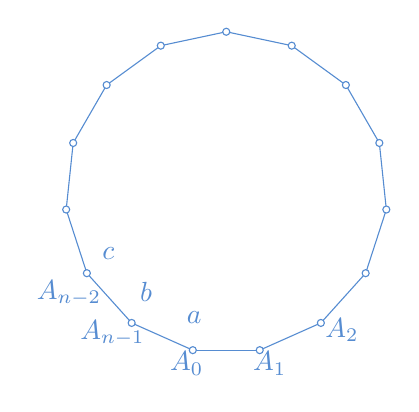
\begin{tikzpicture}[cackithi, scale=0.85, node font= /small]
			\draw  (5.,0.)-- (6.,0.);
			\draw  (6.,0.)-- (6.913545457642599,0.4067366430757997);
			\draw  (6.913545457642599,0.4067366430757997)-- (7.582676064001458,1.1498814685531933);
			\draw  (7.582676064001458,1.1498814685531933)-- (7.891693058376405,2.100937984848346);
			\draw  (7.891693058376405,2.100937984848346)-- (7.787164595108752,3.0954598802166187);
			\draw  (7.787164595108752,3.0954598802166187)-- (7.287164595108752,3.961485284001057);
			\draw  (7.287164595108752,3.961485284001057)-- (6.478147600733806,4.5492705362935295);
			\draw  (6.478147600733806,4.5492705362935295)-- (5.5,4.757182227111289);
			\draw  (5.5,4.757182227111289)-- (4.521852399266196,4.54927053629353);
			\draw  (4.521852399266196,4.54927053629353)-- (3.7128354048912486,3.961485284001059);
			\draw  (3.7128354048912486,3.961485284001059)-- (3.212835404891249,3.0954598802166213);
			\draw  (3.212835404891249,3.0954598802166213)-- (3.108306941623595,2.1009379848483474);
			\draw  (3.108306941623595,2.1009379848483474)-- (3.4173239359985415,1.149881468553195);
			\draw  (3.4173239359985415,1.149881468553195)-- (4.086454542357398,0.4067366430758015);
			\draw  (4.086454542357398,0.4067366430758015)-- (5.,0.);
			\draw [fill=white] (5.,0.) circle (1.5pt);
			\draw (4.91,-0.2) node {$A_0$};
			\draw [fill=white] (6.,0.) circle (1.5pt);
			\draw (6.15,-0.2) node {$A_1$};
			\draw [fill=white] (6.913545457642599,0.4067366430757997) circle (1.5pt);
			\draw (7.23,0.3) node {$A_2$};
			\draw [fill=white] (7.582676064001458,1.1498814685531933) circle (1.5pt);
			\draw [fill=white] (7.891693058376405,2.100937984848346) circle (1.5pt);
			\draw [fill=white] (7.787164595108752,3.0954598802166187) circle (1.5pt);
			\draw [fill=white] (7.287164595108752,3.961485284001057) circle (1.5pt);
			\draw [fill=white] (6.478147600733806,4.5492705362935295) circle (1.5pt);
			\draw [fill=white] (5.5,4.757182227111289) circle (1.5pt);
			\draw [fill=white] (4.521852399266196,4.54927053629353) circle (1.5pt);
			\draw [fill=white] (3.7128354048912486,3.961485284001059) circle (1.5pt);
			\draw (3.15,0.85) node {$A_{n-2}$};
			\draw [fill=white] (3.212835404891249,3.0954598802166213) circle (1.5pt);
			\draw (3.8,0.25) node {$A_{n-1}$};
			\draw [fill=white] (3.108306941623595,2.1009379848483474) circle (1.5pt);
			\draw (3.74,1.45) node {$c$};
			\draw [fill=white] (3.4173239359985415,1.149881468553195) circle (1.5pt);
			\draw (4.3,0.87) node {$b$};
			\draw [fill=white] (4.086454542357398,0.4067366430758015) circle (1.5pt);
			\draw (5.02,0.49) node {$a$};
		\end{tikzpicture}
		\vspace*{-5pt}
	\end{figure}
	Với $n=3k,$ dễ dàng thấy rằng lần lượt viết các số $0, \frac1{2k},\frac1{2k}, 0, \frac1{2k}, \frac1{2k}, 0, \cdots$ theo chiều kim đồng hồ lên các đỉnh sẽ thỏa mãn hai điều kiện trong đầu bài. Như vậy có thể thực hiện được khi và chỉ khi $n$ chia hết cho $3$. Hình vẽ sau đây minh họa cho trường hợp $n=6$.
	\begin{figure}[H]
		\vspace*{-5pt}
		\centering
		\captionsetup{labelformat= empty, justification=centering}
		\begin{tikzpicture}[cackithi,scale=0.85]
			\draw  (3.,0.)-- (5.,0.);
			\draw  (5.,0.)-- (6.,1.7320508075688774);
			\draw  (6.,1.7320508075688774)-- (5.,3.4641016151377553);
			\draw  (5.,3.4641016151377553)-- (3.,3.4641016151377557);
			\draw  (3.,3.4641016151377557)-- (2.,1.732050807568879);
			\draw  (2.,1.732050807568879)-- (3.,0.);
				\draw [fill=white] (3.,0.) circle (1.5pt);
				\draw (2.84,-0.25) node {$0$};
				\draw [fill=white] (5.,0.) circle (1.5pt);
				\draw (5.12,-0.25) node {$\frac{1}{4}$};
				\draw [fill=white] (6.,1.7320508075688774) circle (1.5pt);
				\draw (6.34,1.83) node {$\frac{1}{4}$};
				\draw [fill=white] (5.,3.4641016151377553) circle (1.5pt);
				\draw (5.18,3.85) node {$0$};
				\draw [fill=white] (3.,3.4641016151377557) circle (1.5pt);
				\draw (2.86,3.91) node {$\frac{1}{4}$};
				\draw [fill=white] (2.,1.732050807568879) circle (1.5pt);
				\draw (1.66,1.83) node {$\frac{1}{4}$};
		\end{tikzpicture}
		\vspace*{-10pt}
	\end{figure}
	{\bf\color{cackithi} OC$\pmb{24.}$} Có một bộ $8$ quân cờ domino như trong hình vẽ bên dưới, mỗi quân gồm hai ô vuông đơn vị:
	\begin{figure}[H]
		\vspace*{-5pt}
		\centering
		\captionsetup{labelformat= empty, justification=centering}
		\includegraphics[width= 1\linewidth]{OC24}
		\vspace*{-10pt}
	\end{figure}
	Liệu có thể lát kín hoàn toàn một bảng vuông có kích thước $4 \times 4$ bằng những quân domino này sao cho tổng số chấm trên mỗi hàng, mỗi cột đều bằng nhau?
	\vskip 0.1cm
	\textit{Lời giải.} Có thể lát thỏa mãn điều kiện đầu bài như sau (để đơn giản ta viết số thay cho các chấm trên domino) 
	\begin{figure}[H]
%		\vspace*{-5pt}
		\centering
		\captionsetup{labelformat= empty, justification=centering}
		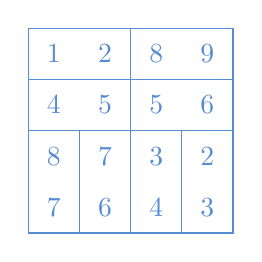
\begin{tikzpicture}[cackithi,scale=0.65, node font=/small]
			\draw (0,0) rectangle (4,4);
			\draw (0,2) -- (4,2) (0,3) -- (4,3) (1,0) -- (1,2) (3,0) -- (3,2) (2,4) -- (2,0);
			\draw (0.5, 0.5) node {$7$};
			\draw (0.5, 1.5) node {$8$};
			\draw (0.5, 2.5) node {$4$};
			\draw (0.5, 3.5) node {$1$};
			\draw (1.5, 0.5) node {$6$};
			\draw (1.5, 1.5) node {$7$};
			\draw (1.5, 2.5) node {$5$};
			\draw (1.5, 3.5) node {$2$};
			\draw (2.5, 0.5) node {$4$};
			\draw (2.5, 1.5) node {$3$};
			\draw (2.5, 2.5) node {$5$};
			\draw (2.5, 3.5) node {$8$};
			\draw (3.5, 0.5) node {$3$};
			\draw (3.5, 1.5) node {$2$};
			\draw (3.5, 2.5) node {$6$};
			\draw (3.5, 3.5) node {$9$};
		\end{tikzpicture}
		\vspace*{-10pt}
	\end{figure}
	Trong phần cuối của chuyên mục kỳ này, chúng tôi sẽ giới thiệu với bạn đọc ba bài toán trong kỳ thi Olympic Toán học Trẻ của Vương quốc Anh năm học $2022$. Các bài toán này phù hợp với trình độ học sinh lớp $6-8$.
	\vskip 0.1cm
	{\bf\color{cackithi} OC$\pmb{31.}$} Bốn góc trong một tứ giác có số đo là các số tự nhiên có $2$ chữ số $\overline{ab}, \overline{cd}, \overline{bd}, \overline{ac}$ như trong hình vẽ. Tìm tất cả các khả năng có thể của tập hợp bốn góc trên.
	\begin{figure}[H]
		\vspace*{-5pt}
		\centering
		\captionsetup{labelformat= empty, justification=centering}
		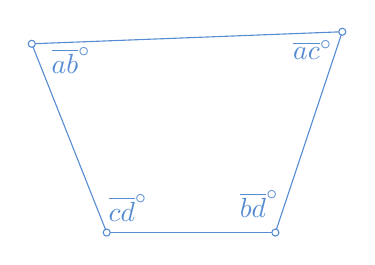
\begin{tikzpicture}[cackithi,scale=0.85, node font= /small]
			\draw  (5.48,-1.)-- (8.,-1.);
			\draw  (8.,-1.)-- (9.,2.);
			\draw  (9.,2.)-- (4.36,1.82);
			\draw  (4.36,1.82)-- (5.48,-1.);
			\draw [fill=white] (5.48,-1.) circle (1.5pt);
			\draw (5.8,-0.63) node {$\overline{cd}^\circ$};
			\draw [fill=white] (8.,-1.) circle (1.5pt);
			\draw (7.76,-0.57) node {$\overline{bd}^\circ$};
			\draw [fill=white] (9.,2.) circle (1.5pt);
			\draw (8.56,1.73) node {$\overline{ac}^\circ$};
			\draw [fill=white] (4.36,1.82) circle (1.5pt);
			\draw (4.95,1.57) node {$\overline{ab}^\circ$};
		\end{tikzpicture}
		\vspace*{-10pt}
	\end{figure}
	{\bf\color{cackithi}OC$\pmb{32.}$} Cho hình ngũ giác đều $ABCDE$. Vẽ hai đường tròn: một có
	tâm $A$ và bán kính $AB$, và hình kia có tâm $B$ và bán kính $BA$. Gọi $X$ là giao điểm bên trong ngũ giác của hai đường tròn.
	Hỏi số đo của $\angle DEX$ bằng bao nhiêu?
	\vskip 0.1cm
	{\bf\color{cackithi}OC$\pmb{33.}$} Seth làm $n$ viên xúc xắc giống hệt nhau bằng cách gấp $n$ bản giống như trong hình bên. Sau đó, anh ta xếp lần lượt các viên xúc xắc chồng lên nhau thành một hình tháp thẳng đứng.
	Biết rằng tổng số chấm ở mỗi một trong bốn mặt xung quanh của tháp xúc xắc đều là số lẻ. Hỏi các giá trị có thể của $n$ là bao nhiêu?
	\begin{figure}[H]
		\vspace*{-5pt}
		\centering
		\captionsetup{labelformat= empty, justification=centering}
		\includegraphics[height= 0.6\linewidth]{OC33}
		\includegraphics[height= 0.6\linewidth]{OC}
		\vspace*{-5pt}
	\end{figure}
\end{multicols}
	\newpage


	\setcounter{figure}{0}
	\thispagestyle{timhieukhoahocnone}
\pagestyle{timhieukhoahoc}
\everymath{\color{timhieukhoahoc}}
\blfootnote{$^1$\text{\color{timhieukhoahoc}Nguồn: Tia Sáng https://tiasang.com.vn/khoa-hoc-cong-nghe/nobel-y-hoc-2022-ky-1-phoi-ngau-voi-ke-thu/.}}
\graphicspath{{../timhieukhoahoc/pic/}}
\begingroup
\AddToShipoutPicture*{\put(0,616){\includegraphics[width=19.3cm]{../bannertimhieu}}}
\AddToShipoutPicture*{\put(130,540){\includegraphics[scale=1]{../tieude.pdf}}}
\centering
\endgroup
\vspace*{160pt}

\begin{multicols}{2}
	Vào đầu tháng $10$ vừa qua, Svante Pääbo được trao giải Nobel Y học “vì những khám phá liên quan đến hệ gene của những nhóm người đã tuyệt chủng và liên quan đến sự tiến hóa của loài người”. Bài viết dưới đây, được đăng trên tạp chí The New Yorker năm $2011$, không lâu sau khi ông công bố bản thảo trình tự hệ gene của người Neanderthal trên Tạp chí Science, làm chấn động thế giới, kể lại hành trình nghiên cứu vừa kỳ lạ, vừa thăng hoa của ông.  
	\begin{figure}[H]
		\vspace*{-5pt}
		\centering
		\captionsetup{labelformat= empty, justification=centering}
		\includegraphics[width= 1\linewidth]{1}
		\caption{\small\textit{\color{timhieukhoahoc}Người Neanderthal. \\Ảnh: Atelier Daynès và S. Entressangle.}}
		\vspace*{-10pt}
	\end{figure}
	\textbf{\color{timhieukhoahoc}Điều gì đã xảy ra giữa chúng ta và những người Neanderthal?}
	\vskip 0.1cm
	Svante Pääbo là người đứng đầu bộ phận di truyền tiến hóa của Viện Max Planck về Nhân chủng Tiến hóa, Leipzig. Ông cao lêu nghêu, khuôn mặt dài, cằm hẹp và có chòm lông mày rậm thường nhướn lên mỗi khi nhấn mạnh một điều gì trái khoáy. Nổi bật trong văn phòng của Pääbo là mô hình bộ xương người Neanderthal kích thước thật, được dựng thẳng đứng lên khiến đôi bàn chân như đang lơ lửng trên mặt đất, và bức chân dung, lớn hơn cả khổ người Pääbo do sinh viên cao học tặng ông vào dịp sinh nhật lần thứ $50$. Mỗi sinh viên vẽ một mảnh của bức tranh và khi ghép lại cho ra một kết quả giống Pääbo một cách kinh ngạc, chỉ mỗi tội là màu sắc không đồng đều khiến chân dung ông trông như bị mắc bệnh ngoài da.
	\vskip 0.1cm
	Dự án tham vọng nhất của Pääbo cho đến nay là tập hợp một nhóm quốc tế để giải trình tự toàn bộ bộ gene của người Neanderthal. Dự án đang hoàn thành một nửa và đã mang lại một số kết quả chưa chắc chắn lắm, bao gồm những tin tức mà Pääbo tung ra vào năm ngoài, đó là người hiện đại, trước khi diệt chủng người Neanderthal, đã giao phối với họ.
	\vskip 0.1cm
	Nếu bộ gene của người Neanderthal được giải trình hoàn chỉnh thì các nhà khoa học có thể đối chiếu từng gene một, từng cặp base một của họ với con người và xem chúng gặp nhau và rẽ nhánh ở đâu. Đến lúc đó, Pääbo tin rằng, câu trả lời cho trăn trở xa xưa sẽ hoàn toàn trong tầm tay.
	\vskip 0.1cm
	Người Neanderthal có quan hệ rất gần gũi người hiện đại -- gần đến mức chúng ta từng đầu gối tay ấp với họ -- và rõ ràng họ không phải con người. Đâu đó nằm giữa những cặp gene khác biệt phải là những đột biến, hay có thể, là những đột biến đã định hình con người chúng ta. Pääbo đã cho một nhóm rà soát hai hệ gene và liệt kê ra những đoạn gene có câu trả lời tiềm năng.
	\vskip 0.1cm
	Pääbo lớn lên ở Stockholm. Mẹ của ông là một nhà hóa học, một người tị nạn Estonia. Bà từng làm việc trong phòng thí nghiệm của nhà hóa sinh Sune Bergström, sau này đã đoạt giải Nobel Y học vào năm $1982$. Pääbo là sản phẩm của một cuộc tình trong phòng thí nghiệm giữa hai người. Mặc dù Pääbo biết cha mình là ai nhưng ông không muốn nhắc đến. Bergström đã có vợ và một con trai khác trong khi mẹ của Pääbo thì chưa bao giờ kết hôn. Vào mỗi thứ bảy, Bergström sẽ đến thăm Pääbo và đưa cậu đi dạo trong rừng hoặc ở một nơi nào khác mà không ai có thể nhận ra ông.
	\vskip 0.1cm
	“Ở nhà coi như ông đi làm vào Thứ Bảy” Pääbo nói với tôi. “Thực sự là việc điên rồ. Vợ ông ấy biết nhưng họ chưa bao giờ nói về nó. Bà không bao giờ gọi cho ông ấy ở nơi làm việc vào các ngày thứ Bảy”. Khi còn nhỏ, Pääbo không đặc biệt bận tâm đến sự sắp xếp này, nhưng sau đó thỉnh thoảng cậu dọa sẽ đến gõ cửa nhà Bergström. “Tôi nói ‘Bố phải nói với con trai của bố vì một lúc nào đó cậu ấy sẽ phát hiện ra’”, ông nhớ lại. Bergström hứa sẽ làm nhưng không bao giờ thực hiện. (Kết quả là người con trai khác của Bergström không biết đến sự tồn tại của Pääbo cho đến trước khi Bergström qua đời vào năm $2004$ không lâu).
	\vskip 0.1cm
	\textbf{\color{timhieukhoahoc}Nghiên cứu bí mật}
	\vskip 0.1cm
	Ngay từ khi còn nhỏ, Pääbo đã thích thú với những thứ cổ cổ. Anh ta phát hiện ra xung quanh những cây đại thụ bị bật gốc có thể tìm thấy những mảnh gốm của người Thụy Điển thời tiền sử, và mang về để đầy căn phòng của mình. Thời thiếu niên một lần được mẹ đưa đến thăm các Kim tự tháp, ông đã bị nó mê hoặc nên sau đó đã đăng ký học Đại học Uppsala và dự định trở thành một nhà Ai Cập học. “Tôi thực sự muốn khám phá những xác ướp, giống như Indiana Jones,” ông nói. Tuy nhiên hầu hết các môn học đều liên quan đến việc phân tích chữ tượng hình, thay vì cảm thấy kích thích thì Pääbo nghĩ nó thật nhàm chán. Được truyền cảm hứng từ cha mình, ông chuyển sang học y rồi sau đó là sinh học tế bào.
	\vskip 0.2cm
	\PIbox{“Điều gì đã khiến chúng ta có thể xây dựng nên những xã hội to lớn này, tỏa ra toàn cầu và phát triển công nghệ mà tôi nghĩ không ai có thể nghi ngờ, là năng lực độc nhất của con người. Phải có một cơ sở di truyền cho điều đó, và nó đang ẩn náu đâu đó trong những đoạn gene này”.
	\vskip 0.1cm
	\hfill \textit{Svante Pääbo}}
	\vskip 0.2cm
	Vào đầu những năm $1980$, khi Pääbo đang làm nghiên cứu sinh về virus thì đột nhiên ông lại mơ tưởng đến xác ướp một lần nữa. Ít nhất là theo hiểu biết của ông lúc bấy giờ, chưa ai tìm cách lấy DNA từ những xác chết cổ đại. Ông tự dưng cảm thấy điều đó là khả thi, và thế là một phương pháp nghiên cứu lịch sử hoàn toàn mới ra đời.
	\vskip 0.1cm
	Sợ rằng thầy hướng dẫn sẽ bảo ý tưởng này là ngớ ngẩn (hoặc tệ hơn thế) nên Pääbo đã bí mật tiến hành nghiên cứu xác ướp, vào ban đêm. Nhờ quen một giáo sư Ai Cập học, ông đã tìm được một số mẫu vật từ Bảo tàng Ai Cập ở Đông Berlin. Năm $1984$, ông công bố kết quả của mình trên một tạp chí Đông Đức ít người biết đến. Ông công bố đã phát hiện được DNA trong tế bào của một đứa trẻ được ướp xác đã chết hơn $2{.}000$ năm. Pääbo kỳ vọng có thể tìm được lời giải đáp cho những câu hỏi như điều gì đã khiến các triều đại Pharaon thay đổi và mẹ của Tutankhamun là ai từ DNA của các xác ướp này.
	\vskip 0.1cm
	Trong lúc soạn thảo phiên bản tiếng Anh của bài báo thì một nhóm các nhà khoa học Đại học California tại Berkeley thông báo rằng họ đã thành công trong việc giải trình tự một đoạn DNA từ một động vật giống ngựa vằn được gọi là quagga, một loài thú đã bị săn bắn đến tuyệt chủng vào những năm $1880$. (DNA này được lấy từ xác con thú hơn $140$ năm tuổi được bảo quản tại Bảo tàng Lịch sử Quốc gia Mainz). Trưởng nhóm Berkeley, Allan Wilson là một nhà hóa sinh có tiếng tăm. Ông là người tìm ra phương pháp nghiên cứu sự tiến hóa sử dụng khái niệm “đồng hồ phân tử”. Pääbo liền gửi cho Wilson một số đoạn trong bài báo xác ướp của mình. Wilson rất ấn tượng và ngỏ ý hỏi có còn vị trí nào trống trong lab của Pääbo; ông muốn dành kỳ sabatical (nghỉ phép để nghiên cứu) ở đó. Pääbo trả lời Wilson rằng mình không thể cho Wilson một vị trí nào ở phòng lab cả, vì đáng tiếc là anh nào có lab đâu -- thậm chí lúc đó còn chưa có bằng tiến sỹ nữa kìa.
	\begin{figure}[H]
		\vspace*{-5pt}
		\centering
		\captionsetup{labelformat= empty, justification=centering}
		\includegraphics[width= 1\linewidth]{2}
		\caption{\small\textit{\color{timhieukhoahoc}Nhóm nghiên cứu của Svante Pääbo. \\Ảnh: mpg.de}}
		\vspace*{-10pt}
	\end{figure}
	Bài báo về xác ướp của Pääbo được công bố trên trang bìa tạp chí \textit{Nature}. Tờ \textit{New York Times} còn viết về nó, gọi đây là “công trình kịch tính nhất trong một loạt các thành tựu gần đây của sinh học phân tử”. Dẫu vậy, các đồng nghiệp của Pääbo ở Thụy Điển vẫn tỏ ra hoài nghi. Họ giục ông hãy quên đi những xác chết nhăn nheo và kiên định với virus. “Tất cả nọi người đều nói với tôi rằng thật là ngu xuẩn khi rời bỏ một lĩnh vực quan trọng để đến với một thứ gần giống như trò tiêu khiển”. Pääbo phớt lờ họ, đến Berkeley làm việc cho Wilson.
	\vskip 0.1cm
	\textbf{\color{timhieukhoahoc}Một ngành khoa học mới}
	\vskip 0.1cm
	“Anh ấy lên cứ như diều gặp gió” -- Mary--Claire King, người cũng từng là sinh viên của Wilson và hiện là giáo sư về khoa học genome tại Đại học Washington, nhớ là Pääbo và Wilson (ông qua đời năm $1991$). “Cả hai đều nghĩ về những ý tưởng rất lớn”. “Và mỗi người đều rất giỏi trong việc chuyển những ý tưởng đó thành những giả thuyết có thể kiểm chứng được. Cả hai cũng rất giỏi trong việc phát triển công nghệ cần thiết để kiểm tra các giả thuyết. Có được cả ba năng lực đó thì quả là đáng nể ”. Ngoài ra, tuy nhiên “dù cả hai đều rất coi trọng dữ liệu nhưng ai cũng không ngần ngại nói những điều phóng đại về dữ liệu của mình, và đều không hề sợ sai”.
	\vskip 0.1cm
	DNA bao gồm các phân tử được gọi là nucleotide đan lại với nhau theo hình bậc thang -- chính là chuỗi xoắn kép nổi tiếng. Mỗi nucleotide chứa một trong bốn base: Adenine, Thymine, Guanine và Cytosine được ký hiệu bằng các chữ cái A, T, G và C. Do đó một đoạn của bộ gene người có thể được biểu thị là ACCTCCTCTAATGTCA. Bộ gene của con người là một dải ba tỷ cặp base. Theo những gì đã xác định đến giờ này, thì phần lớn các cặp base đều không đáng quan tâm.
	\vskip 0.1cm
	Ngoại trừ các tế bào hồng cầu thì mọi tế bào trong một sinh vật đều chứa một bản sao hoàn chỉnh của DNA của nó. Nó cũng chứa nhiều bản sao, từ hàng trăm đến hàng nghìn, của một dạng DNA rút gọn được gọi là DNA ty thể (mtDNA). Nhưng ngay sau khi sinh vật chết thì các chuỗi nucleotide dài bắt đầu bị phá vỡ. Phần lớn diễn ra trong vài giờ đầu tiên bởi các enzym bên trong cơ thể của chính sinh vật. Sau một thời gian, tất cả những gì còn lại là các đoạn mã, và sau một thời gian nữa -- phụ thuộc vào các điều kiện phân hủy -- những đoạn mã này cũng tan rã. “Có lẽ trong lớp băng vĩnh cửu bạn có thể quay ngược lại năm trăm nghìn năm,” Pääbo nói với tôi. “Nhưng chắc chắn trong giới hạn một triệu năm thôi.” Năm trăm nghìn năm trước thì loài khủng long cũng đã tuyệt chủng được hơn $64$ triệu năm nên toàn bộ hình dung về “công viên kỷ Jura”, đáng tiếc, chỉ dừng lại ở tưởng tượng. Thế nhưng, năm trăm nghìn năm trước thì con người hiện đại vẫn chưa ra đời.
	\vskip 0.2cm
	\PIbox{
	“Pääbo đã đưa lĩnh vực nghiên cứu DNA cổ đại, vốn ban đầu chỉ là chuyện giả tưởng trong phim ‘Công viên kỷ Jura’ thành một khoa học thực sự, đó là một thành tựu lớn”.
	\vskip 0.1cm
	\hfill \textit{Maynard Olson}}
	\vskip 0.2cm
	Khi đến California, Pääbo vẫn quan tâm đến hướng sử dụng di truyền học để nghiên cứu lịch sử loài người. Tuy nhiên trong khi cố gắng xác định vị trí các đoạn ADN của người Ai Cập cổ đại, ông đã phát hiện ra một vấn đề lớn: chúng trông rất giống -- thực sự, giống hệt -- các đoạn ADN của con người đương đại. Vì vậy phân tử vi mô trên da của ông hoặc của người khác, thậm chí là của giám tuyển bảo tàng đã qua đời từ lâu tình cờ rơi vào, cũng có thể phá hỏng công sức cả tháng trời làm việc.
	\vskip 0.1cm
	Ông giải thích: “Rõ ràng là tạp nhiễm từ bên ngoài là một vấn đề lớn. (Cuối cùng, Pääbo kết luận rằng các trình tự mà mình thu được trong bài báo xác ướp ban đầu của mình có thể đã bị hỏng vì lý do này). Và để khởi động, ông bắt đầu nghiên cứu những loài động vật đã tuyệt chủng. Ông phân tích mẫu mtDNA từ những con lười khổng lồ trên mặt đất đã biến mất khoảng mười hai nghìn năm trước như voi ma mút hay hổ Tasmania, bị săn bắn đến tuyệt chủng vào thập niên $1930$. Ông cũng trích xuất mtDNA từ moas, loài chim khổng lồ không biết bay sống ở New Zealand trước khi người Maori đến, và nhận thấy rằng moas có quan hệ họ hàng gần với các loài chim từ Úc hơn là kiwi, loài chim không bay sống ở New Zealand ngày nay. Ông cũng thăm dò rất nhiều xác sinh vật không có DNA nào hữu ích, như xương từ công viên cổ sinh La Brea (nơi có hàng ngàn sinh vật thời kỳ băng hà bị chôn trong nhựa đường) và côn trùng hóa thạch được bảo quản trong hổ phách. Trong quá trình làm việc này, Pääbo ít nhiều đã phát minh ra lĩnh vực cổ sinh học.
	\vskip 0.1cm
	“Thành thật mà nói đây là vấn đề mà bản thân tôi sẽ không muốn giải quyết, vì tôi nghĩ nó quá khó,” Maynard Olson, giáo sư danh dự tại Đại học Washington và một trong những người sáng lập Dự án Genome người Neanderthal đã nói với tôi. “Pääbo đã mang lại những tiêu chuẩn rất cao cho lĩnh vực này, và đưa lĩnh vực nghiên cứu DNA cổ đại, vốn ban đầu chỉ là chuyện giả tưởng trong phim ‘Công viên kỷ Jura’ thành một khoa học thực sự, đó là một thành tựu lớn”.
	\begin{figure}[H]
		\vspace*{-5pt}
		\centering
		\captionsetup{labelformat= empty, justification=centering}
		\includegraphics[width= 1\linewidth]{3}
		\caption{\small\textit{\color{timhieukhoahoc}Các nhà nghiên cứu phải rất cẩn trọng để tránh chính DNA của mình làm tạp nhiễm những mẩu xương cổ đại.}}
		\vspace*{-10pt}
	\end{figure}
	Ed Green, giáo sư kỹ thuật phân tử sinh học tại Đại học California ở Santa Cruz, người làm việc trong Dự án bộ Gene người Neanderthal cho biết: “Hầu hết các ngành khoa học đều không có gì đặc biệt. Nếu bạn không làm, thì vài tháng sau sẽ có người khác làm về lĩnh vực đó. Svante là một trong số những nhà khoa học hiếm hoi chứng minh điều ngược lại. Nếu không có ông, sẽ không có ngành DNA cổ đại như chúng ta đã biết”.
	\vskip 0.1cm
	\textbf{\color{timhieukhoahoc}Bước ngoặt trong nghiên cứu}
	\vskip 0.1cm
	Trong thời gian Pääbo sống ở California, thỉnh thoảng ông đến Đức để thăm một phụ nữ đang học cao học tại Đại học Munich. “Tôi đã có nhiều bạn trai, nhưng nhiều lúc tôi cũng có bạn gái”, ông nói với tôi. Khi mối quan hệ này kết thúc, thì ngay sau đó, Đại học Munich đã đề nghị Pääbo làm trợ lý giáo sư. Vì không có lý do thúc ép nào để chuyển đến Đức nên ông do dự. Rồi đề nghị đó trở thành lời mời làm giáo sư toàn phần: “Và rồi tôi nói, ồ chắc nước Đức cũng không tệ lắm đâu. Tôi sẽ đến đó vài năm”.
	\vskip 0.1cm
	Khi bảo tàng Bang Rhenish, ở Bonn gọi Pääbo nhiều năm sau đó, ông vẫn đang yên vị ở Munich. Bảo tàng này lưu giữ xương của người Neanderthal đầu tiên được xác định, được phát hiện vào mùa hè năm $1856$. Ông nghĩ mình có bao bao nhiêu \% cơ hội để trích xuất những DNA hữu ích từ đó? Pääbo chỉ có thể xác định được tình trạng những chiếc xương cho đến khi ông tìm đến chúng.
	\vskip 0.1cm
	“Tôi không biết phải nói gì với họ, vì vậy tôi nói,” Có $5\%$ cơ hội có thể tìm ra”, ông nhớ lại. Vài tháng sau, ông nhận được một phần nhỏ của hài cốt bên phải của người Neanderthal.
	\vskip 0.1cm
	Người Neanderthal đầu tiên được tìm thấy trong một hang động đá vôi cách Bonn khoảng bốn mươi lăm dặm về phía Bắc, trong một khu vực được gọi là Thung lũng Neander, theo tiếng Đức là das Neandertal. Mặc dù hang động đã biến mất -- đá vôi từ lâu đã được khai thác để phục vụ xây dựng -- khu vực này bây giờ là một công viên giải trí theo chủ đề người Neanderthal với bảo tàng riêng, những con đường mòn đi bộ đường dài và một khu vườn trồng các loại cây bụi đã xuất hiện từ kỷ băng hà. Người Neanderthal ở đây được khắc họa như những con người dễ mến, nếu không muốn nói là cuốn hút. Lối vào tòa nhà là một mô hình người Neanderthal cao tuổi đang chống gậy. Bên cạnh ông ta là một trong những điểm tham quan nổi tiếng nhất của bảo tàng -- một phòng chụp ảnh tên là Morphing-Station. Với $3$ euro, khách đến đây sẽ được nhận một bức ảnh chụp chân dung họ bình thường, một bức ảnh thứ hai, đối xứng với bức thứ nhất, được chỉnh sửa với cằm thụt vào trong, trán hếch và sau đầu phồng ra. Lũ trẻ thích tự nhìn mình -- hay đặc biệt là chứng kiến anh chị em chúng -- bị biến hình thành người Neanderthal. Chúng thấy buồn cười kinh lên được.
	\vskip 0.1cm
	Những bộ xương đầu tiên của người Neanderthal xuất hiện ở Thung lũng Neander bị đối xử như rác rưởi. Các mảnh vỡ như nắp sọ, bốn xương cánh tay, hai xương đùi và một phần xương chậu, về sau được một doanh nhân địa phương thu vén lại. Anh ta lại nghĩ rằng đó là xương của một con gấu tiền sử và gửi đến cho một người sưu tập hóa thạch. Người thu thập hóa thạch nhận ra rằng đây là một thứ lạ lẫm hơn nhiều so với một con gấu, một “thành viên nguyên thủy của chủng tộc chúng ta”.
	\vskip 0.1cm
	\PIbox{
	Trước khi “thay thế” người Neanderthal, con người hiện đại đã quan hệ tình dục với họ. Sự mắc mứu này đã sinh ra những đứa trẻ, trở thành những công dân của châu Âu, châu Á và Tân Thế giới.}
	\vskip 0.1cm
	Và rồi điều này xảy ra đúng vào khoảng thời gian Darwin xuất bản cuốn “Về nguồn gốc của các loài”, và các mảnh xương nhanh chóng trở thành chủ đề tranh luận về nguồn gốc của con người. Những người phản đối thuyết tiến hóa khăng khăng rằng chúng thuộc về một người bình thường. Một giả thuyết cho rằng đó là một người Cossack đã lưu lạc đến khu vực trong cuộc hỗn loạn sau Chiến tranh Napoléon. Lý do bộ xương trông kỳ lạ -- xương đùi của người Neanderthal bị cong một cách đặc trưng -- là người Cossack đã ngồi quá lâu trên ngựa. Một người khác cho rằng hài cốt là của một người đàn ông bị bệnh còi xương: người đàn ông này đã phải chịu đựng quá nhiều cơn đau vì căn bệnh của mình đến mức khiến trán của anh ta luôn căng ra -- do đó, một phần xương trán bị nhô ra. (Nhưng không ai thấy phân vân khi một người đã còi xương và thường xuyên đau đớn lại leo trèo vào hang động làm~gì).
	\vskip 0.1cm
	Trong những thập kỷ tiếp theo, những bộ xương giống xương của người ở Thung lũng Neander -- dày hơn xương của người hiện đại, với những hộp sọ có hình dạng kỳ lạ -- đã được phát hiện tại một số địa điểm khác bao gồm hai ở Bỉ và một ở Pháp. Trong khi đó một hộp sọ được khai quật nhiều năm trước đó ở Gibraltar được cho là trông rất giống với hộp sọ tìm thấy ở Đức. Rõ ràng tất cả những thứ còn sót lại này không thể được giải thích bằng chuyện về người Cossack lạc đường hay người còi xương đi thám hiểm hang động nữa. Nhưng các nhà tiến hóa cũng không biết giải thích thế nào. Người Neanderthal có hộp sọ rất lớn -- trung bình lớn hơn người hiện đại ngày nay. Điều này khiến chúng ta khó có thể đưa họ vào trong quá trình tiến hóa từ loài vượn có não nhỏ tiến lên những bộ não lớn hơn cho đến con người. Trong cuốn “Hậu duệ của con người” xuất bản năm $1871$, Darwin chỉ đề cập đến người Neanderthal rất ngắn. “Phải thừa nhận rằng một số hộp sọ có tính rất cổ xưa, chẳng hạn như hộp sọ nổi tiếng của người Neanderthal, đã phát triển tốt và có năng lực,” ông lưu ý.
	\vskip 0.1cm
	Năm $1908$, một bộ xương gần như hoàn chỉnh của người Neanderthal được phát hiện trong một hang động gần La Chapelle--aux--Saints, miền Nam nước Pháp. Bộ xương đã được gửi đến một nhà cổ sinh vật học tên là Marcellin Boule thuộc Bảo tàng Lịch sử Tự nhiên Quốc gia Paris. Trong một loạt sách chuyên khảo, Boule đã phát minh ra thứ tạm gọi là bức biếm họa về người Neanderthal -- đầu gối cong, lưng gù và tàn bạo. Boule viết: các xương của người Neanderthal thể hiện một “cấu trúc linh trưởng đặc trưng”, và hình dạng hộp sọ cho thấy đây là “một loài kém phát triển hoặc hung tợn”. Các kết luận của Boule được nhiều người cùng thời với ông nghiên cứu và lặp lại; Ví dụ, nhà nhân chủng học người Anh, Sir Grafton Elliot Smith, đã mô tả người Neanderthal đi đứng với “một cơ thể khùng khoằm” đặt trên “một đôi chân đặc biệt dị dạng” (Smith còn mô tả người Neanderthal thêm muôn phần xấu xí với gần như toàn thân lông lá dù đến nay chưa hề có bằng chứng rõ ràng nào cho thấy họ nhiều lông).
	\vskip 0.1cm
	Vào những năm $1950$, hai nhà giải phẫu học Williams Straus và Alexander Cave quyết định kiểm tra lại bộ xương từ La Chapelle. Straus và Cave khẳng định rằng những gì Boule tưởng là dáng đi tự nhiên của người Neanderthal, thực ra là do bệnh viêm khớp. Người Neanderthal không đi bộ với tư thế còng lưng và khuỵu chân. Thật vậy, nếu cạo râu nhẵn nhụi và khoác một bộ cánh mới và bước vào tàu điện ngầm ở New York thì một người Neanderthal có lẽ sẽ chả khiến ai chú ý “hơn một số cư dân khác của thành phố này”, họ viết. Nhiều nghiên cứu gần đây có xu hướng ủng hộ ý tưởng như vậy.
	\vskip 0.1cm
	Pääbo quyết định giải trình tự toàn bộ hệ gene của người Neanderthal vào tháng $7/2006$ đúng vào dịp kỷ niệm $155$ năm phát hiện ra người Neanderthal. Thông báo được đưa ra cùng với một công ty của Mỹ, $454$ Life Sciences, công ty đã phát triển một máy giải trình tự “thông lượng cao” với sự trợ giúp của các quả cầu nhựa nhỏ, có thể tái tạo hàng chục nghìn đoạn DNA cùng một lúc. Cả trong và ngoài ngành di truyền học kế hoạch này được xem là vô cùng tham vọng và dự án đã gây tiếng vang trên toàn thế giới. “Một nghiên cứu thật to gan”, tiêu đề trên tờ \textit{The Economist} tuyên bố.
	\vskip 0.1cm
	\textbf{\color{timhieukhoahoc}Con đường chông gai}
	\vskip 0.1cm
	Giờ đây, một phiên bản hoàn chỉnh của bộ gene người đã được công bố. Cùng với đó là các phiên bản hệ gene khác của tinh tinh, chuột, chuột cống cũng hoàn thành. Nhưng con người, tinh tinh, chuột và chuột cống đều là sinh vật sống, trong khi người Neanderthal đã tuyệt chủng trong ba mươi nghìn năm. Rào cản đầu tiên chỉ đơn giản là tìm đủ DNA của người Neanderthal để giải trình tự. Mẫu vật còn lại của người Neanderthal mà Pääbo nhận được ban đầu đã mang lại một số thông tin di truyền nhưng còn xa mới đủ số lượng cần thiết để lắp ráp/tập hợp lại cho đủ toàn bộ bộ gene. Vì vậy, Pääbo đã đặt hy vọng của mình vào một nhóm xương khác từ Croatia. (Xương của người Croatia hóa ra thuộc về ba người, tất cả đều là phụ nữ; người Neanderthal ban đầu có lẽ là đàn ông).
	\vskip 0.1cm
	Đến cuối năm $2006$, Pääbo và nhóm của ông báo cáo rằng bằng cách sử dụng một mảnh xương của người Croatia, họ đã thành công trong việc giải trình tự một triệu cặp base của bộ gene người Neanderthal. (Cũng giống như bộ gene của con người, bộ gen đầy đủ của người Neanderthal bao gồm khoảng ba tỷ cặp cơ bản). Ngoại suy ra họ ước tính sẽ mất khoảng hai năm và sáu nghìn lần “chạy” trên một cỗ máy $454$ Life Sciences để hoàn thành dự án. Nhưng phân tích sau đó cho thấy hàng triệu cặp base có thể đã bị tạp nhiễm bởi DNA của con người. Điều này khiến một số nhà di truyền học đặt câu hỏi liệu Pääbo có vội vàng công bố những kết quả mà lẽ ra anh ta phải biết là sai hay không. Trong khi đó, các xương tiếp theo mang lại tỷ lệ DNA Neanderthal thấp hơn nhiều và tỷ lệ DNA vi sinh vật cao hơn nhiều. (Khoảng $80\%$ DNA đã giải trình tự trong Dự án bộ gene người Neanderthal đều thuộc về vi sinh vật và, theo dự án thì hoàn toàn là vô dụng). Điều này có nghĩa là, công sức để hoàn thiện bộ gene lớn hơn rất nhiều so với những ước tính ban đầu. “Đã có những lúc tuyệt vọng,” Pääbo nói với tôi. Giải quyết được vấn đề này thì lại nảy ra vấn đề khác. “Đó là một chuyến tàu lượn đầy cảm xúc,” Ed Green, kỹ sư phân tử sinh học từ Santa Cruz, nhớ lại.
	\vskip 0.1cm
	Khoảng sau hai năm bắt đầu dự án, một thách thức nảy sinh. Pääbo đã tập hợp một nhóm quốc tế để giúp phân tích dữ liệu từ các máy giải trình tự -- về cơ bản, là một danh sách dài của A, T, G, C. Đang sàng lọc dữ liệu thì một trong những thành viên của nhóm, David Reich, một nhà di truyền học tại Trường Y Harvard, đã nhận thấy điều kỳ lạ. Trình tự của người Neanderthal, đúng như dự đoán, rất giống với trình tự của con người. Nhưng có những kiểu người giống với người Neanderthan hơn những kiểu người khác. Cụ thể, người châu Âu và châu Á chia sẻ DNA với người Neanderthal nhiều hơn người châu Phi. “Chúng tôi đã cố gắng phủ nhận kết quả này”, Reich nói với tôi. “Chúng tôi đã nghĩ, không thể thế~được”.
	\vskip 0.1cm
	Trong khoảng $25$ năm qua, nghiên cứu về sự tiến hóa của loài người đã bị chi phối bởi lý thuyết được báo chí đại chúng gọi là “Từ châu Phi mà ra” (Out of Africa), hay giới học thuật gọi là giả thuyết “nguồn gốc duy nhất gần đây” hoặc giả thuyết “thay thế”. Lý thuyết này cho rằng tất cả con người hiện đại đều là hậu duệ của một nhóm dân số nhỏ sống ở châu Phi khoảng hai trăm nghìn năm trước. (Không lâu trước khi ông qua đời, Allan Wilson, cố vấn của Pääbo đã phát triển một trong những bằng chứng quan trọng cho lý thuyết, dựa trên sự so sánh DNA ty thể của người đương đại). Khoảng một trăm hai mươi nghìn năm trước một nhóm nhỏ người đã di cư vào Trung Đông, và đến năm mươi nghìn năm trước, một nhóm con khác đã đi vào lục địa Âu--Á. Khi di chuyển về phía Bắc và phía Đông, con người hiện đại chạm trán với người Neanderthal và những người khác được gọi là “người cổ đại”, những người đã sinh sống ở những vùng này trước đó. Con người hiện đại đã “thay thế” con “người cổ đại”, thật là một xảo ngôn che giấu việc con người đã đẩy họ đến tuyệt chủng. Mô hình di cư và “thay thế” này ngụ ý rằng dù đến từ đâu thì con người và người Neanderthal cũng có mối quan hệ (thù địch) với nhau.
	\vskip 0.1cm
	Nhiều thành viên trong nhóm của Pääbo những tưởng đó là một trường hợp nhiễm tạp khác. Nhiều khi các mẫu xử lý bởi người châu Âu; đã bị trộn DNA của họ với DNA của người Neanderthal. Người ta đã chạy một số thử nghiệm để đánh giá khả năng này. Các kết quả đều âm tính. Reich nói với tôi: “Chúng tôi tiếp tục nhìn thấy đặc tính này và càng có nhiều dữ liệu xác nhận nó về mặt thống kê. Dần dần, các thành viên khác trong nhóm bắt đầu suy nghĩ. Trong một bài báo đăng trên tạp chí \textit{Science}, vào tháng $5/2010$, họ đã giới thiệu điều mà Pääbo gọi là giả thuyết “thay thế bị rò rỉ”. (Bài báo sau đó được bình chọn là bài báo xuất sắc của năm và nhóm nghiên cứu đã nhận được giải thưởng $25$ nghìn USD).
	\vskip 0.1cm
	Giả thuyết “thay thế bị rò rỉ” -- giả định rằng nó đúng vào lúc này -- cung cấp thêm bằng chứng về sự gần gũi của người Neanderthal với con người hiện đại. Không chỉ cả hai đã giao phối với nhau, mà những đứa con lai cũng đủ cứng cáp để hòa nhập vào xã hội loài người. Một số con lai này sống sót để có những đứa con của riêng mình, đến lượt chúng, lại sinh con, và cứ thế cho đến ngày nay. Ngay cả bây giờ, ít nhất là ba mươi nghìn năm sau sự kiện này, tín hiệu này vẫn không thể khiến chúng ta làm ngơ: tất cả những người không có nguồn gốc châu Phi, từ người New Guinea đến người Pháp cho đến người Hán Trung Hoa đều mang đâu đó từ một đến bốn phần trăm DNA của người Neanderthal.
	\vskip 0.1cm
	Khi cuối cùng Pääbo có thể đón nhận ý tưởng rằng, người Neanderthal trao lại một số gene của họ cho người hiện đại, ông nói với tôi, “Tôi nghĩ điều đó thật “cool”. Nó có nghĩa là họ không hoàn toàn bị tuyệt chủng -- mà vẫn còn hiện hữu phảng phất trong cơ thể chúng ta”. 
	\vskip 0.1cm
	\hfill\textit{(còn tiếp)}
	\vskip 0.1cm
	\hfill Nguyễn Quang \textit{dịch}\footnote[2]{\color{timhieukhoahoc} Nguyên tác: https://www.newyorker.com/magazine/2011/08/15/sleeping-with-the-enemy}
\end{multicols}




	\newpage
	
	\setcounter{figure}{0}
	 \thispagestyle{gocconone}
\pagestyle{gocco}
\everymath{\color{gocco}}
\graphicspath{{../gocco/pic/}}
\blfootnote{$^1${\color[named]{gocco}Trung tâm Quy hoạch và Điều tra tài nguyên -- môi trường biển khu vực phía Nam.}}
\begingroup
\AddToShipoutPicture*{\put(0,616){\includegraphics[width=19.3cm]{../bannergocco}}}
\AddToShipoutPicture*{\put(106,522){\includegraphics[scale=1]{../tieude2.pdf}}} 
\centering
\endgroup

\vspace*{185pt}
\begin{multicols}{2}
	``\textit{Biết giấu mình dưới chín lớp đất cũng bằng biết khuấy động chín tầng trời}". Khi bắt đầu bước vào mỗi cuộc chiến cân não, nhiệm vụ quan trọng của đôi bên không chỉ là tìm cách bắt Tướng đối phương mà còn cần phải bảo vệ sự an toàn của Tướng của mình bằng những cách khéo léo và thông minh nhất. Để trở thành người chơi cờ giỏi, ngoài khả năng điều động quân lực, uy hiếp tấn công lên trận địa đối phương, các kỳ thủ cần sở hữu một kỹ năng không kém phần quan trọng, đó chính là Phòng thủ.
	\vskip 0.1cm
	Tuy vậy, tâm lý khi lâm trận của mỗi người thường muốn giành lấy chiến thắng càng nhanh càng tốt, nóng lòng hình thành thế tiến công ngay từ ban đầu khiến cho đối phương không kịp trở tay. Và nếu quá chăm chú vào mặt trận tấn tấn công mà lơ là mặt trận phòng thủ, hoặc phòng thủ một cách sơ sài, thiếu kế hoạch theo quan niệm ``\textit{Tấn công là cách phòng thủ tốt nhất}" thì chắc chắn sẽ để lộ ra những yếu điểm chết người, không thể giành thắng lợi mà còn tạo cơ hội cho đối phương phản kích dễ dàng.
	\vskip 0.1cm
	Trong bài viết kỳ này, tác giả sẽ gửi đến những hình cờ điển hình để bạn đọc Pi có thể hiểu hơn về tầm quan trọng của kỹ năng phòng thủ: 
	\vskip 0.1cm
	$1$.	Hình $1$, Đỏ còn chiến Xe rất mạnh và được đi tiên Đen chỉ còn Mã, Chốt và Tượng, Đỏ đi những nước mang tính uy hiếp như sau:  
	\begin{figure}[H]
		\vspace*{-5pt}
		\centering
		\captionsetup{labelformat= empty, justification=centering}
		\includegraphics[width= 0.4\textwidth]{1}
		\caption{\small\textit{\color{gocco}Hình $1$.}}
		\vspace*{-10pt}
	\end{figure}
	$\pmb{1)}$	X$5-2$ M$3.5$\quad $\pmb{2)}$ X$2.6$ Tg$5.1$\quad $\pmb{3)}$ X$2/1$ Tg$5/1$\quad $\pmb{4)}$ X$2/1$ Tg$5.1$\quad $\pmb{5)}$ X$2/1$ M$5/7$\quad $\pmb{6)}$ X$2-3$ Tg$/1$\quad $\pmb{7)}$ X$3.1$ ($*$) Tg$.1$\quad $\pmb{8)}$ Tg$5.1$ M$3.5$ $(**)$  ($1/2$)
	\vskip 0.1cm
	\textit{$(*)$: Dựa vào sức mạnh tuyệt đối của Xe, Đỏ liên tục tung ra những đòn quấy rối cực kỳ khó chịu. Tương ứng với đó Đen cũng đưa ra những đáp trả rất chính xác.
	\vskip 0.1cm
	$(**)$: Nếu trong tình huống thông thường cũng với số lượng quân như vậy, Đỏ sẽ dễ dàng giành chiến thắng. Tuy nhiên với hình cờ cụ thể này, những quân của Đen đã có vị trí rất đẹp và vận dụng kỹ năng phòng thủ rất thuần thục, các quân liên kết một cách hợp lý, tạo ra bức tường không thể khoan phá. Ván đấu có kết quả hòa là hoàn toàn xác đáng.}
	\begin{figure}[H]
		\vspace*{-5pt}
		\centering
		\captionsetup{labelformat= empty, justification=centering}
		\includegraphics[width= 0.4\textwidth]{2}
		\caption{\small\textit{\color{gocco}Hình $2$.}}
		\vspace*{-10pt}
	\end{figure}
	$2.$ Hình $2$, đôi bên đang có quân lực như nhau, tuy nhiên Đỏ nắm lợi thế vì Xe Chốt đang áp sát, sẵn sàng lấy mạng Tướng đối phương bất cứ khi nào. Trong thế đi hậu liệu Đen có thể thủ hòa thành công ? Diễn biến tiếp theo của cuộc cờ như sau: 
	\vskip 0.1cm
	$\pmb{1)}$	X$4-6$ $(*)$ X$5-6$ \quad $\pmb{2)}$ Tg$4-5$ Tg$5-6$ $(**)$\quad $\pmb{3)}$ C$7-6$  X$6-8$ $(***)$\quad $\pmb{4)}$ X$6-5$ X$8-5$\quad $\pmb{5)}$ Tg$5-6$ X$5-4$\quad $\pmb{6)}$ Tg$6-5$ X$4/3$ $(****)$ ($1/2$)
	\vskip 0.1cm
	\textit{$(*)$: Với lợi thế đi tiên, Đỏ ngay lập tức bình Xe sang trục lộ $6$ hòng tạo điều kiện cho Chốt lộ $7$ xâm nhập cửu cung một cách dễ dàng hơn.
	\vskip 0.1cm
	$(**)$: Đen cũng không hề chịu thua kém, ngay lập tức bình Xe rồi bình Tướng qua trục còn lại chiếm con đường huyết mạch. 
	\vskip 0.1cm
	$(***)$: Mặc dù Đỏ có bình chốt áp sát, Đen vẫn bình tĩnh đưa Xe sang lộ $8$ -- một nước chờ đợi đầy kinh nghiệm. Nếu ở đây Đen vội vàng tấn Chốt nhằm tìm cơ hội đối công thì sẽ phải trả giá rất đắt, Đỏ đi X$4-5$, Đen thua ngay lập tức.
	\vskip 0.1cm
	$(****)$: Mặc dù Đỏ chỉ còn $1$ nước nữa là có thể bình Chốt tạo sát, nhưng Đen cũng có những nước đáp trả đầy mẫu mực. Đôi bên chỉ còn đơn Xe, ván đấu kết thúc với kết quả hòa.}
	\begin{figure}[H]
		\vspace*{-5pt}
		\centering
		\captionsetup{labelformat= empty, justification=centering}
		\includegraphics[width= 0.4\textwidth]{3}
		\caption{\small\textit{\color{gocco}Hình $3$.}}
		\vspace*{-10pt}
	\end{figure}
	$3.$ Hình $3$, Quân lực của Đỏ đang áp đảo nhưng Đen chỉ cần một nước nữa là có thể tạo ra sát cục. Trong tình thế cực kỳ nguy cấp, Đỏ đã liên tiếp tung ra những đòn phế quân để thủ hòa như sau:
	\vskip 0.1cm
	$\pmb{1)}$ Xt$.1$ S$5/4$\quad $\pmb{2)}$ X$6.2$ Tg$5.1$\quad $\pmb{3)}$ X$6-5$ Tg$5-6$\quad $\pmb{4)}$ M$5/3$ P$7/5$\quad $\pmb{5)}$ X$5/8$ $(*)$ P$7-4$\quad $\pmb{6)}$ P$3-6$ C$4-5$\quad $\pmb{7)}$ P$6-7$ C$5.1$ $(**)$\quad $\pmb{8)}$ P$7/5$ C$4-5$\quad $\pmb{9)}$ P$7-5$ $(***)$ ($1/2$)
	\vskip 0.1cm
	$(*)$: Trong thế không còn gì để mất, Đỏ đã liên tục bỏ quân, trước phế Xe, sau hiến Mã khiến cho Đen chưa thể kết thúc ván cờ. Tranh thủ thời gian quý báu đó, Đen lui về tiêu trừ Chốt $5$ của Đen và chiếm lấy vị trí đắc địa để phòng thủ.
	\vskip 0.1cm
	$(**)$: Dù đã mất quân Chốt quý giá, Đen vẫn đủ lực, sử dụng Pháo Chốt để tạo một đợt tấn công khác. Sau khi tấn Chốt chém Xe Đỏ, Đen tiếp tục dọa sát.
	\vskip 0.1cm
	$(***)$: Đen vẫn có những nước phòng thủ vô cùng hợp lý. Tuy vẫn còn một chút lợi thế nhưng chừng đó là chưa đủ để Đen giành chiến thắng.
	\vskip 0.1cm
	\textit{Chú thích}: C: Chốt, X: Xe, M: Mã, P: Pháo, Tg: Tướng, S: Sĩ, T: Tượng, t: trước.
	\vskip 0.1cm
	\textbf{\color{gocco}Câu đố kỳ này:}  Đôi bên sẽ vận dụng khả năng điều quân như thế nào để giữ vững trận địa trong những hình cờ đối công dưới đây (bên Đỏ được quyền đi trước)?
	\begin{figure}[H]
		\vspace*{-5pt}
		\centering
		\captionsetup{labelformat= empty, justification=centering}
		\includegraphics[width= 0.4\textwidth]{4}
		\caption{\small\textit{\color{gocco}Hình $4$.}}
		\vspace*{-10pt}
	\end{figure}
	\textit{Đáp án}: $\pmb{1)}$ C$5-6$ M$7/5$\quad $\pmb{2)}$ C$6.1$ T$3/5$\quad $\pmb{3)}$ C$2-3$ C$6-5$ \quad $\pmb{4)}$ Tg$5-4$ M$5.7$\quad $\pmb{5)}$ X$5-3$ C$5.1$\quad $\pmb{6)}$ Tg$4.1$ C$4-5$\quad $\pmb{7)}$ Tg$4-5$ C$7.1$ ($1/2$)
	\begin{figure}[H]
		\vspace*{-5pt}
		\centering
		\captionsetup{labelformat= empty, justification=centering}
		\includegraphics[width= 0.4\textwidth]{5}
		\caption{\small\textit{\color{gocco}Hình $5$.}}
		\vspace*{-10pt}
	\end{figure}
	\textit{Đáp án}: $\pmb{1)}$ X$4-5$ Tg$5.1$\quad $\pmb{2)}$ C$7-6$ X$4/1$\quad $\pmb{3)}$ C$4.1$ Tg$5/1$\quad $\pmb{4)}$ P$7.8$ S$4.5$\quad $\pmb{5)}$ C$4.1$ S$5/6$\quad $\pmb{6)}$ P$7-4$ Tg$5.1$\quad $\pmb{7)}$ X$8-5$ Tg$5/1$\quad $\pmb{8)}$ P$4-1$ Tg$5.1$\quad $\pmb{9)}$ P$1/1$ Tg$5/1$\quad $\pmb{10)}$ P$1-6$ Tg$5-4$ ($1/2$).
\end{multicols}





	\newpage
	
%	\thispagestyle{empty}
%	\begingroup 
%	\AddToShipoutPicture*{\put(0,0){\includegraphics[width=19.3cm]{dovui.pdf}}}
%	\centering
%	\vspace*{0cm}
%	\endgroup
%	\newpage	
%	\pagestyle{empty}
\end{document} 

%	\setcounter{figure}{0}
%\thispagestyle{lichsutoanhocnone}
\pagestyle{lichsutoanhoc}
\graphicspath{{../lichsutoanhoc/pic2/}}
\everymath{\color{lichsutoanhoc}}
\blfootnote{$^1$\color{lichsutoanhoc}Cộng tác viên Viện Toán học.}
\begingroup
\AddToShipoutPicture*{\put(0,616){\includegraphics[width=19.3cm]{../bannerlichsu}}}
\AddToShipoutPicture*{\put(60,470){\includegraphics[scale=1]{../tieude3.pdf}}}
\centering
\endgroup

\vspace*{236pt}

\begin{multicols}{2}
	$\pmb{1}$. \textbf{\color{lichsutoanhoc}Democritus xứ Abdera} 
	\vskip 0.1cm
	Xã hội loài người đã và đang trải qua năm giai đoạn phát triển: Tiền sử (Prehistory), Cổ đại (Classical), Trung đại (Middle), Cận đại (Early Modern) và Hiện đại (Modern). \textit{Thời đại anh hùng} thuộc vào thời kỳ Cổ đại. Trong thời đại anh hùng, đặc biệt là ở Hy Lạp và La Mã, các vị thần và á thần, các anh hùng vĩ đại trong truyền thuyết (Achilles, Hercules, Agamemnon, ...)  đã thực hiện những hành động anh hùng và tỏa sáng. 
	\vskip 0.1cm
	Thời đại anh hùng đã tạo ra nửa tá nhân vật vĩ đại trong toán học, trong số đó phải kể đến Democritus xứ Abdera (khoảng $460-370$ TCN), ngày nay được tôn vinh như một người đề xướng học thuyết duy vật nguyên tử, nhưng đương thời ông cũng được tôn vinh như một nhà hình học. Ông được cho là đã đi du lịch nhiều hơn bất kỳ ai trong thời của mình -- ông đã đến Athens, Ai Cập, Lưỡng Hà và có thể cả Ấn Độ -- tiếp thu những gì học được, và những thành tựu của riêng ông trong toán học là xuất sắc. Ông đã viết một số công trình toán học, nhưng ngày nay không còn tồn tại. 
	\vskip 0.1cm
	Chìa khóa cho toán học của Democritus được tìm thấy trong học thuyết vật lý về nguyên tử. Ông lập luận, về mức độ nhỏ vô hạn và đa dạng vô hạn (về kích thước và hình dạng), các nguyên tử di chuyển không ngừng trong không gian trống.
	\vskip 0.1cm 
	Thuyết vật lý nguyên tử của Democritus có thể đã xuất phát từ thuyết nguyên tử hình học của Pythagoras, và không có gì ngạc nhiên khi các vấn đề toán học mà Democritus quan tâm chủ yếu là những thứ đòi hỏi cách tiếp cận đại lượng vô cùng bé. Ví dụ, người Ai Cập nhận thức được rằng thể tích của một kim tự tháp bằng một phần ba tích của đáy và chiều cao, nhưng chứng minh điều này gần như chắc chắn nằm ngoài khả năng của họ, vì nó đòi hỏi các kiến thức giải tích.  Archimedes đã viết rằng kết quả này là của Democritus.  Archimedes cũng gán cho Democritus định lý nói  rằng thể tích của một hình nón bằng một phần ba thể tích của hình trụ tròn ngoại tiếp. Kết quả này có lẽ đã được Democritus coi là hệ quả của định lý về kim tự tháp, vì hình nón về cơ bản là một hình chóp có đáy là một đa giác đều có vô số cạnh.
	\vskip 0.1cm
	Lý thuyết nguyên tử hình học của Democritus ngay lập tức đối đầu với nhiều vấn đề. Ví dụ: Nếu các phần liền kề có diện tích bằng nhau, thì vì tất cả các phần đều bằng nhau, tổng sẽ là một lăng trụ hoặc một hình trụ và không phải là một hình chóp hoặc một hình nón. 
	\vskip 0.1cm
	Mặt khác, nếu các phần liền kề không bằng nhau, tổng sẽ là một kim tự tháp có bậc hoặc một hình nón có bậc chứ không phải là hình có bề mặt nhẵn. Vấn đề này không giống như những khó khăn với số vô tỷ và với những nghịch lý của chuyển động.
	\vskip 0.1cm
	Có lẽ, trong tác phẩm \textit{On the Irrational} (về Vô tỷ), Democritus đã phân tích những khó khăn gặp phải, nhưng không có cách nào để biết những nỗ lực của ông có thể đã đi theo hướng nào.
	\vskip 0.1cm
	Sự không được ưa chuộng của Democritus trong hai trường phái triết học thống trị thế kỷ tiếp theo, của Plato và Aristotle, có thể đã khuyến khích việc coi thường các ý tưởng của Democritus. 
	\vskip 0.1cm
	Di sản toán học chính của Thời đại anh hùng có thể được tóm gọn trong sáu vấn đề: cầu phương hình tròn, nhân đôi thể tích hình lập phương, chia ba một góc, tỷ lệ giữa các đại lượng không thông ước, các nghịch lý về chuyển động, và phương pháp vô cùng bé. 
	\vskip 0.1cm
	Những bài toán này liên quan, ở mức độ nào đó, với những người cùng thời: Hippocrates, Archytas, Hippias, Hippasus, Zeno và Democritus. 
	\vskip 0.1cm
	Những thời đại khác nhau tạo ra một loạt tài năng có thể so sánh được, nhưng có lẽ không có thời đại nào có thể thực hiện một cuộc tấn công táo bạo vào rất nhiều các vấn đề toán học với nguồn tài nguyên phương pháp luận không đầy đủ như vậy. Vì lý do này mà thời kỳ từ Anaxagoras đến Archytas được gọi là ``thời đại anh hùng" trong toán học.
	\vskip 0.1cm
	$\pmb{2.}$ \textbf{\color{lichsutoanhoc}Eudoxus}
	\vskip 0.1cm
	 Nhà toán học Hy Lạp lỗi lạc nhất trước Archimedes có lẽ là Eudoxus xứ Cnidos ($408 - 355$ TCN).
	 \vskip 0.1cm
	Ra đời khoảng năm $408$ TCN ở Cnidos trên Biển Đen, ở tuổi $23$, Eudoxus bắt đầu học hình học với Archytas xứ Tarentum, và học triết học và hùng biện với Plato ở Athens. Eudoxus, quá nghèo để sống ở Athens, đã ở trọ với giá rẻ mạt tại thị trấn bến cảng Piraeus, mỗi ngày ông phải đi bộ hai dặm ($1$ dặm = $1{,}6$ km) đến Học viện Plato. Sau đó, ông đến Ai Cập, nơi ông ở lại trong $16$ tháng. Ông kiếm sống bằng nghề dạy học, thành lập một trường học tại Cyzicus ở Tây Bắc Tiểu Á, trường đã thu hút rất nhiều học sinh. Vào năm $365$ TCN, Eudoxus trở lại Athens cùng với một lượng lớn các học trò. Ở đó, ông trở thành một đồng nghiệp của Plato.
	Eudoxus cũng đã mở một trường học ở Athens, có một thời gian là đối thủ cạnh tranh của Học viện Plato.
	\vskip 0.1cm
	Eudoxus là nhà toán học và thiên văn học hàng đầu của thời đại mình. Eudoxus đã giải quyết những khủng hoảng của toán học thời đại ông. Ông có ba cống hiến cho toán học: lý thuyết tổng quát về tỷ lệ, bổ sung nhiều kết quả nghiên cứu về tỷ lệ vàng, và phát minh ra một quy trình được gọi là \textit{phương pháp vét kiệt}.
	\vskip 0.1cm 
	\textbf{\color{lichsutoanhoc}Lý thuyết tổng quát về tỷ lệ} 
	\vskip 0.1cm
	Việc khám phá ra số vô tỷ đã gây ra một sự khủng hoảng trong toán học, vì nó đã làm lung lay niềm tin về số (hữu tỷ) là bản chất của mọi thứ và làm lý thuyết về tỷ lệ của người Pythagoras không còn vững vàng. Hai đại lượng, chẳng hạn như đường chéo và cạnh của hình vuông, không thông ước, vì độ dài của chúng không có tỷ lệ là một số (hữu tỷ). Vậy thì làm thế nào để so sánh các tỷ lệ của các đại lượng vô ước?
	\vskip 0.1cm
	Người Pythagoras đã sử dụng ý tưởng rằng bốn đại lượng theo tỷ lệ, $a:b = c : d$  nếu hai tỷ lệ $a:b$  và $c:d$ bằng nhau có thể thay thế nhau. Nghĩa là, tỷ lệ nhỏ hơn trong mỗi tỷ lệ có thể được áp dụng cho tỷ lệ lớn hơn cùng một số lần và phần còn lại trong mỗi trường hợp có thể bị bỏ đi trên cùng một số nguyên lần nhỏ hơn, và phần mới còn lại có thể được thay thế trên phần còn lại cũ cùng một số nguyên lần, v.v. 
	\vskip 0.1cm
	Định nghĩa như vậy rất khó sử dụng (khi áp dụng cho số vô tỷ), do đó lý thuyết mới về tỷ lệ là một thành tựu rực rỡ của Eudoxus và nó đã được đưa vào Quyển V của \textit{Cơ sở} của Euclid.
	\vskip 0.1cm
	Một tuyên bố quan trọng của Euclid là các đại lượng được cho có một tỷ lệ với nhau nếu bội số của một trong hai số có thể vượt quá số kia. 
	\vskip 0.1cm
	Đây thực chất là tiên đề Archimedes -- mà Archimedes gán cho Eudoxus. Khái niệm tỷ lệ của Eudoxus do đó loại trừ số không và làm rõ nghĩa độ lớn cùng loại là gì. Ví dụ: một đoạn thẳng không được so sánh theo tỷ lệ với diện tích; cũng như diện tích không được so sánh với thể tích.
	\vskip 0.1cm
	Sau những nhận xét sơ bộ về tỷ lệ, Euclid đưa ra Định nghĩa $5$ trong Quyển V của \textit{Cơ sở} về phát biểu nổi tiếng của Eudoxus: \textit{Các độ lớn được cho là theo cùng một tỷ lệ, tỷ lệ cái thứ nhất trên cái thứ hai và cái thứ ba với cái thứ tư, khi nào, nếu có bằng bất kỳ thứ gì được lấy từ đầu tiên và thứ ba, và bằng cái thứ hai và cái thứ tư, các điểm bằng nhau trước đây đều vượt quá, giống nhau bằng, hoặc là giống nhau nhỏ hơn, các bội số sau được lấy theo thứ tự tương ứng} ([$4$], trang $80$, xem thêm [$5$], trang $236$).
	\vskip 0.1cm
	Nghĩa là, $\dfrac{a}{b} = \dfrac{c}{d}$  nếu và chỉ nếu với các số nguyên dương bất kỳ $m$  và $n$,  nếu $ma < mb$,  thì $mc < nd$,  hoặc nếu $ma = nb$,  thì $mc = nd$,  hoặc $ma > mb$  thì $mc > nd$. 
	\vskip 0.1cm
	Định nghĩa của Eudoxus về sự bằng nhau của tỷ lệ không khác gì phép nhân chéo được sử dụng ngày nay cho phân số $\dfrac{a}{b} = \dfrac{c}{d}$  -- một sự tương đương với việc đưa về mẫu số chung.  Ví dụ, để chứng tỏ rằng $\dfrac{3}{6}$  bằng $\dfrac{4}{8}$  ta nhân $3$ và $6$ với $4$, được $12$ và $24$, và nhân $4$ và $8$ với $3$, thu được cùng một cặp số $12$ và $24$.
	\vskip 0.1cm 
	Cần lưu ý rằng, định nghĩa này không xa mấy so với định nghĩa về số thực ở thế kỷ $19$ bởi lát cắt Dedekind, vì nó phân lớp số hữu tỷ  $\dfrac{m}{n}$  thành hai lớp, theo $ma \le nb$  và $ma > nb$.
	\vskip 0.1cm 
	Vì có vô số số hữu tỷ, người Hy Lạp đã phải đối mặt với khái niệm mà họ muốn tránh--đó là tập hợp vô hạn -- nhưng ít nhất dựa trên khái niệm về tỷ lệ của Eudoxus, họ đã có thể đưa ra các chứng minh thỏa đáng cho các định lý liên quan đến tỷ lệ.
	\vskip 0.1cm
	\textbf{\color{lichsutoanhoc}Phương pháp vét kiệt}
	\vskip 0.1cm
	Cuộc khủng hoảng về vô ước đã được giải quyết thành công, nhờ vào định nghĩa của Eudoxus về tỷ lệ, nhưng vẫn còn một vấn đề chưa được giải quyết -- so sánh cấu hình đường cong và đường thẳng. 
	\vskip 0.1cm
	Ở đây, có vẻ như Eudoxus đã cung cấp chìa khóa.
	\vskip 0.1cm
	Các nhà toán học trước đây dường như đã có ý mô tả các hình đa giác nội tiếp và ngoại tiếp các hình cong và tiếp tục tăng vô hạn số cạnh, nhưng họ đã không biết cách lập luận, vì khái niệm giới hạn là chưa rõ ràng vào thời điểm ấy. 
	\vskip 0.1cm
	Theo Archimedes, chính Eudoxus là người đã cung cấp bổ đề hiện mang tên Archimedes -- đôi khi được gọi là tiên đề về tính liên tục -- được dùng làm cơ sở cho phương pháp vét kiệt, tương đương với tiếng Hy Lạp của phép tính tích phân.
	\vskip 0.1cm
	Bổ đề (hoặc tiên đề) Eudoxus nói rằng hai đại lượng có một tỷ số (nghĩa là, không bằng $0$) nếu có thể tìm thấy một nhân tử để đại lượng này sẽ vượt quá đại lượng kia. Có thể phát biểu điều này trên ngôn ngữ hiện đại như sau: Cho $M > \epsilon$  và một số $0 < r < 1$. Khi ấy tồn tại số $n \in \mathbb{N}$  sao cho $M(1-r)^n < \epsilon$, tức là $\mathop {\lim }\limits_{n \to \infty } M{\left( {1 - r} \right)^n} = 0$. 
	\vskip 0.1cm
	Khẳng định này đã loại trừ lập luận mơ hồ về các đoạn thẳng không thể phân chia hoặc các số nhỏ cố định, đôi khi duy trì trong tư tưởng Hy Lạp. 
	\vskip 0.1cm
	Phương pháp vét kiệt được đề xuất bởi Eudoxus sau đó đã được Archimedes phát triển thành một công cụ mạnh mẽ để xác định diện tích hình phẳng, diện tích bề mặt và thể tích đường cong --  một tiền thân quan trọng của phép toán tích phân.
	\begin{figure}[H]
		\vspace*{-5pt}
		\centering
		\captionsetup{labelformat= empty, justification=centering}
		\includegraphics[width= 1\linewidth]{1}
		\vspace*{-15pt}
	\end{figure}
	\textbf{\color{lichsutoanhoc}Thiên văn của Eudoxus} 
	\vskip 0.1cm
	Eudoxus không chỉ là một nhà toán học. Ông còn được biết đến như là cha đẻ của khoa học thiên văn. Plato được cho là đã cố gắng đưa ra một biểu diễn hình học về chuyển động của Mặt Trời, Mặt Trăng và năm hành tinh đã biết. Rõ ràng là người ta ngầm cho rằng các chuyển động là hợp nhất của các chuyển động tròn đều. Mặc dù có những hạn chế như vậy, Eudoxus đã có thể cung cấp cho mỗi thiên thể trong số bảy thiên thể một biểu diễn thỏa đáng thông qua một tổ hợp các quả cầu đồng tâm với tâm là Trái Đất và với các bán kính khác nhau, mỗi quả cầu quay đều quanh một trục cố định đối với bề mặt của hình cầu lớn hơn tiếp theo. Với mỗi hành tinh thì Eudoxus đưa ra một hệ thống mà những người kế vị của ông biết đến là ``Hình cầu đồng tâm". Những sơ đồ hình học này, được kết hợp bởi Aristotle vào vũ trụ học, đã thống trị tư tưởng trong gần $2000$ năm.
	\vskip 0.1cm
	Eudoxus, không nghi ngờ gì, là nhà toán học có năng lực nhất Thời kỳ Hy Lạp hóa (Hellenic period, khoảng $507 - 323$ trước Công nguyên), nhưng tất cả các tác phẩm của ông đã bị thất lạc. Trong thiên văn học, bằng sự kết hợp của các chuyển động tròn, Eudoxus đã có thể mô tả chuyển động của các hành tinh trong các quỹ đạo lặp lại dọc theo một đường cong được gọi là con hà mã, hoặc vòng kiềng ngựa. Đường cong này, giống như một hình số tám trên một hình cầu, là một trong số ít các đường cong mới mà người Hy Lạp đã tìm ra. Vào thời điểm đó, chỉ có hai phương tiện xác định các đường cong: ($1$) thông qua sự kết hợp của các chuyển động đều và ($2$) như các giao điểm của các bề mặt hình học quen thuộc. 
	\vskip 0.1cm
	Proclus, khoảng $800$ năm sau Eudoxus, nói rằng Eudoxus đã thêm nhiều định lý tổng quát trong hình học và đã áp dụng phương pháp phân tích của Plato để nghiên cứu tỷ lệ vàng, nhưng cống hiến lớn nhất của  Eudoxus vẫn là lý thuyết về tỷ lệ và phương pháp vét kiệt.
	\vskip 0.1cm
	$\pmb{3.}$ \textbf{\color{lichsutoanhoc}Phép suy luận suy diễn và Đại số hình học}
	\vskip 0.1cm 
	Thales có lẽ là người đầu tiên nhận thấy nhu cầu về một phương pháp suy luận hợp lý chặt chẽ. Một số nhà nghiên cứu cho rằng, hình thức suy luận suy diễn hình thành muộn hơn nhiều -- thậm chí có thể là vào đầu thế kỷ thứ tư TCN, sau khi phát hiện ra số vô tỷ. 
	\vskip 0.1cm
	Các đề xuất khác tìm nguyên nhân bên ngoài toán học. Một ví dụ là suy luận suy diễn có thể đã xuất phát từ logic, trong nỗ lực thuyết phục một phản đối của một kết luận bằng cách tìm kiếm các tiền đề mà từ đó kết luận nhất thiết phải tuân theo.
	\vskip 0.1cm
	Liệu suy luận có được đưa vào toán học vào thế kỷ VI TCN hay thế kỷ IV TCN và liệu tính không thông ước đã được phát hiện trước đó hoặc sau năm $400$ TCN? Không thể nghi ngờ rằng toán học Hy Lạp đã trải qua những thay đổi mạnh mẽ vào thời của Plato. Sự phân đôi giữa số (number) và độ lớn liên tục (continuous magnitude) đòi hỏi một cách tiếp cận mới đối với Đại số Babylon mà người Pythagoras đã kế thừa.
	\vskip 0.1cm
	Các bài toán cũ trong đó, cho tổng và tích các cạnh của hình chữ nhật, các thứ nguyên được yêu cầu phải được xử lý khác với thuật toán số của người Babylon. 
	\vskip 0.1cm
	Một ``đại số hình học" phải thay thế cho 11đại số số học" cũ và trong đại số mới này không thể  thêm cạnh vào diện tích hoặc thêm diện tích vào thể tích.
	\vskip 0.1cm
	Kể từ bây giờ, phải có một sự đồng nhất nghiêm ngặt của các thuật ngữ trong các phương trình, thí dụ, $xy = A, y \pm x = b$, với diễn giải về mặt hình học. Để tìm $y$ và $x$  ta phải xây dựng trên một cạnh cho trước $b$  một hình hình chữ nhật có chiều rộng $x$  chưa biết sao cho diện tích của hình chữ nhật vượt quá diện tích $A$  đã cho bởi hình vuông  $x^2$ (trường hợp $xy = A, y + x = b$, Hình $1$ bên trái) hoặc rút ngắn diện tích  $A$ bởi hình vuông  $x^2$ (trường hợp $xy = A, y - x = b$,  Hình $1$ bên phải). 
	\begin{figure}[H]
		\vspace*{-5pt}
		\centering
		\captionsetup{labelformat= empty, justification=centering}
		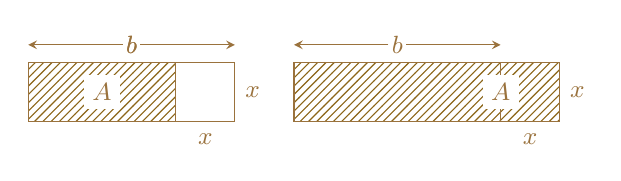
\begin{tikzpicture}[lichsutoanhoc,scale=0.75, node font = \small]
			\draw (0,0) rectangle (3.5,1);
			\draw[pattern=north east lines, pattern color= lichsutoanhoc] (0,0) rectangle (2.5,1);
			\draw (4.5,0) rectangle (9,1);
			\draw[pattern=north east lines, pattern color= lichsutoanhoc] (4.5,0) rectangle (9,1);
			\draw (8,0) -- (8,1);
			\draw (1.25,0.5) node[fill = white]{$A$};
			\draw (8,0.5) node[fill = white]{$A$};
			\draw (1.75, 1.3) node {$b$};
			\draw (1.75, 1.3) node {$b$};
			\draw (6.25, 1.3) node {$b$};
			\draw[-stealth] (1.6,1.3) -- (0, 1.3);
			\draw[-stealth] (1.9,1.3) -- (3.5, 1.3);
			\draw[-stealth] (6.1,1.3) -- (4.5, 1.3);
			\draw[-stealth] (6.4,1.3) -- (8, 1.3);
			
			\draw (3, -0.3) node {$x$};
			\draw (3.8, 0.5) node {$x$};
			\draw (8.5,-0.3) node {$x$};
			\draw (9.3, 0.5) node {$x$};
		\end{tikzpicture}
		\caption{\small\textit{\color{lichsutoanhoc}Hình $1$.}}
		\vspace*{-10pt}
	\end{figure}
	Theo cách này, người Hy Lạp đã xây dựng lời giải của phương trình bậc hai bằng một quá trình được gọi là ``ứng dụng của diện tích", một phần của đại số hình học được trình bày chi tiết trong \textit{Cơ sở} của Euclid. 
	\vskip 0.1cm
	Hơn nữa, sử dụng các đoạn thẳng dẫn đến việc tránh các tỷ lệ, trong chừng mực có thể, trong toán sơ cấp. Thí dụ, phương trình tuyến tính $ax = bc$ được coi là một đẳng thức của các diện tích $ax$  và $bc$,  thay vì theo tỷ lệ -- một đẳng thức giữa hai tỷ số $a : b$  và $c : x$. Do đó, khi xây dựng tỷ lệ thứ tư, $x$  trong trường hợp này, thông thường ta dựng một hình chữ nhật $OCDB$  với các cạnh $b = OB$  và  $c = OC$ (Hình $2$) và sau đó dọc theo $OC$  đặt $OA = a$.  Được hình chữ nhật $OAEB$ và vẽ đường chéo $OE$  cắt  $CD$ tại $P$.  Bây giờ rõ ràng  $CP$ là đoạn  $x$ mong muốn, và hình chữ nhật  $OARS$ có diện tích bằng hình chữ nhật $OCDB$. 
	\begin{figure}[H]
		\vspace*{-5pt}
		\centering
		\captionsetup{labelformat= empty, justification=centering}
		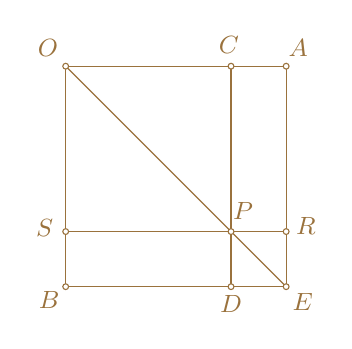
\begin{tikzpicture}[lichsutoanhoc,scale=0.7, node font = \small]
			\draw  (0.,0.)-- (4.,0.);
			\draw  (4.,0.)-- (4.,4.);
			\draw  (4.,4.)-- (0.,4.);
			\draw  (0.,4.)-- (0.,0.);
			\draw  (0.,1.)-- (3.,1.);
			\draw  (3.,1.)-- (3.,4.);
			\draw  (3.,4.)-- (0.,4.);
			\draw  (0.,4.)-- (0.,1.);
			\draw  (0.,4.)-- (4.,0.);
			\draw  (3.,1.)-- (4.,1.);
			\draw  (3.,1.)-- (3.,0.);
			\draw [fill=white] (0.,0.) circle (1.5pt);
			\draw (-0.3,-0.25) node {$B$};
			\draw [fill=white] (4.,0.) circle (1.5pt);
			\draw (4.3,-0.27) node {$E$};
			\draw [fill=white] (4.,4.) circle (1.5pt);
			\draw (4.22,4.33) node {$A$};
			\draw [fill=white] (0.,1.) circle (1.5pt);
			\draw (-0.38,1.07) node {$S$};
			\draw [fill=white] (3.,1.) circle (1.5pt);
			\draw (3.22,1.37) node {$P$};
			\draw [fill=white] (3.,4.) circle (1.5pt);
			\draw (2.96,4.39) node {$C$};
			\draw [fill=white] (0.,4.) circle (1.5pt);
			\draw (-0.32,4.33) node {$O$};
			\draw [fill=white] (4.,1.) circle (1.5pt);
			\draw (4.36,1.11) node {$R$};
			\draw [fill=white] (3.,0.) circle (1.5pt);
			\draw (3.,-0.31) node {$D$};
		\end{tikzpicture}
		\caption{\small\textit{\color{lichsutoanhoc}Hình $2$.}}
		\vspace*{-10pt}
	\end{figure}
	Mãi đến Quyển V của \textit{Cơ sở} Euclid mới giải quyết vấn đề khó khăn về tỷ lệ.
	\vskip 0.1cm
	Đại số hình học Hy Lạp là quá mức nhân tạo và khó khăn đối với các độc giả hiện đại. Tuy nhiên, nó có vẻ là một công cụ tiện lợi cho những người đã sử dụng nó và trở nên thành thạo trong việc xử lý các hoạt động của nó.
	\vskip 0.1cm
	Luật phân phối $a(b + c + d) = ab + ac + ad$  chắc chắn là rõ ràng hơn đối với một học giả Hy Lạp hơn là sinh viên ngày nay, vì trước đây có thể dễ dàng hình dung các diện tích của hình chữ nhật trong định lý này, nói một cách đơn giản rằng hình chữ nhật trên $a$ và tổng của các đoạn $b,c,d$  bằng tổng các hình chữ nhật trên $a$  và mỗi các cạnh $b,c,d$  được lấy riêng (Hình $3$). 
	\begin{figure}[H]
		\vspace*{-5pt}
		\centering
		\captionsetup{labelformat= empty, justification=centering}
		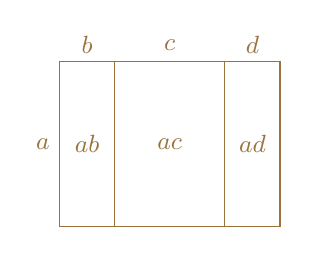
\begin{tikzpicture}[lichsutoanhoc,scale=0.7, node font = \small]
			\draw (0,0) rectangle (4,3);
			\draw (1,0) -- (1, 3) (3,0) -- (3,3);
			\draw (-0.3, 1.5) node {$a$};
			\draw (0.5, 1.5) node {$ab$};
			\draw (2, 1.5) node {$ac$};
			\draw (3.5, 1.5) node {$ad$};
			\draw (0.5, 3.3) node {$b$};
			\draw (2, 3.3) node {$c$};
			\draw (3.5, 3.3) node {$d$};
		\end{tikzpicture}\quad
		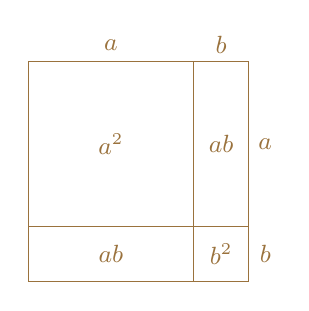
\begin{tikzpicture}[lichsutoanhoc,scale=0.7, node font = \small]
			\draw  (0.,0.)-- (4.,0.);
			\draw  (4.,0.)-- (4.,4.);
			\draw  (4.,4.)-- (0.,4.);
			\draw  (0.,4.)-- (0.,0.);
			\draw  (0.,1.)-- (3.,1.);
			\draw  (3.,1.)-- (3.,4.);
			\draw  (3.,4.)-- (0.,4.);
			\draw  (0.,4.)-- (0.,1.);
			\draw  (3.,1.)-- (4.,1.);
			\draw  (3.,1.)-- (3.,0.);
			\draw (1.5,0.5) node {$ab$};
			\draw (4.3,0.5) node {$b$};
			\draw (3.5,4.3) node {$b$};
			\draw (1.5,2.5) node {$a^2$};
			\draw (1.5,4.3) node {$a$};
			\draw (3.5,2.5) node {$ab$};
			\draw (4.3,2.5) node {$a$};
			\draw (3.5,0.5) node {$b^2$};
		\end{tikzpicture}
		\caption{\small\textit{\color{lichsutoanhoc}\hfill Hình $3$ \hfill\hfill Hình $4$ \hfill}}
		\vspace*{-10pt}
	\end{figure}
	Một lần nữa, hệ thức $(a+ b)^2 = a^2 + 2ab + b^2$  trở nên hiển nhiên từ sơ đồ cho thấy ba hình vuông và hai hình chữ nhật bằng nhau trong Hình $4$; và hiệu của hai hình vuông $a^2 - b^2 = (a + b)(a-b)$  có thể được minh họa tương tự, như trong Hình $5$. 
	\begin{figure}[H]
		\vspace*{-5pt}
		\centering
		\captionsetup{labelformat= empty, justification=centering}
		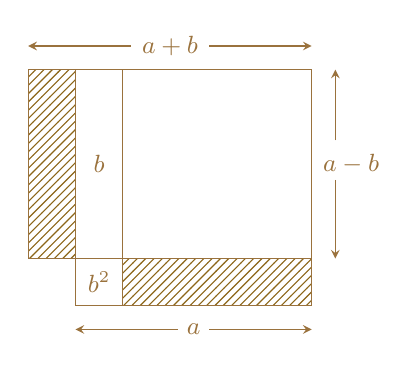
\begin{tikzpicture}[lichsutoanhoc, node font = \small]
			\draw (0,0) rectangle (3,3);
			\draw (0.6,0.6) rectangle (3,3);
			\draw[pattern=north east lines, pattern color= lichsutoanhoc] (0.6,0) rectangle (3,0.6);
			\draw[pattern=north east lines, pattern color= lichsutoanhoc] (0,0.6) rectangle (-0.6,3);
			\draw (0,0.6) -- (0.6,0.6);
			\draw (0.3,0.3) node {$b^2$};
			\draw (0.3,1.8) node {$b$};
			\draw (1.5,-0.3) node {$a$};
			\draw (3.5,1.8) node {$a-b$};
			\draw (1.2,3.3) node {$a +b$};
			\draw [-stealth] (0.7,3.3) -- (-0.6,3.3);
			\draw [-stealth] (1.7,3.3) -- (3,3.3);
			\draw [-stealth] (1.3,-0.3) -- (0,-0.3);
			\draw [-stealth] (1.7,-0.3) -- (3,-0.3);
			\draw [-stealth] (3.3,2.1) -- (3.3,3);
			\draw [-stealth] (3.3,1.6) -- (3.3,0.6);
		\end{tikzpicture}
		\caption{\small\textit{\color{lichsutoanhoc}Hình $5$.}}
		\vspace*{-10pt}
	\end{figure}
	Tổng, hiệu, tích và thương của các đoạn thẳng có thể dễ dàng được xây dựng bằng một thước thẳng và một compass.  
	\vskip 0.1cm
	Căn bậc hai cũng không gặp khó khăn trong đại số hình học.  Muốn tìm một đoạn $x$  sao cho $x^2 = ab$, ta chỉ cần làm theo cách có thể tìm thấy trong sách giáo khoa hình học ngày nay: Lấy đoạn thẳng  $ABC$, trong đó $AB = a$  và $BC = b$  (Hình $6$). Với $AC$ là đường kính, người ta dựng một nửa hình tròn (tâm  $O$) và tại $B$  dựng  $BP$ vuông góc với $AC$. $BP$ là đoạn  $x$ cần tìm. 
	\begin{figure}[H]
		\vspace*{-5pt}
		\centering
		\captionsetup{labelformat= empty, justification=centering}
		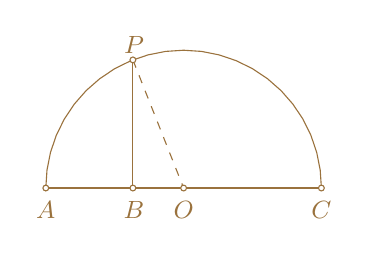
\begin{tikzpicture}[lichsutoanhoc, scale=0.7, node font = \small]
			\draw [shift={(1.5,1.)}]  plot[domain=0.:3.141592653589793,variable=\t]({1.*2.5*cos(\t r)+0.*2.5*sin(\t r)},{0.*2.5*cos(\t r)+1.*2.5*sin(\t r)});
			\draw  (-1.,1.)-- (4.,1.);
			\draw  (0.58,3.3245644753372616)-- (0.58,1.);
			\draw[dashed]  (0.58,3.3245644753372616)-- (1.5,1.);
			\draw [fill=white] (-1.,1.) circle (1.5pt);
			\draw (-1,0.6) node {$A$};
			\draw [fill=white] (4.,1.) circle (1.5pt);
			\draw (4,0.6) node {$C$};
			\draw [fill=white] (1.5,1.) circle (1.5pt);
			\draw (1.5,0.6) node {$O$};
			\draw [fill=white] (0.58,1.) circle (1.5pt);
			\draw (0.6,0.6) node {$B$};
			\draw [fill=white] (0.58,3.3245644753372616) circle (1.5pt);
			\draw (0.6,3.6) node {$P$};
		\end{tikzpicture}
		\caption{\small\textit{\color{lichsutoanhoc}Hình $6$.}}
		\vspace*{-10pt}
	\end{figure}
	Điều thú vị ở đây là, Euclid đã chỉ ra, có thể tránh tỷ lệ bằng cách sử dụng các diện tích.
	\vskip 0.1cm
	Nếu trong Hình $6$ đặt $PO = AAO = CO =r$  và $BO = s$,  khi ấy ta có 
	\begin{align*}
		x^2 = r^2 - s^2 = (r-s)(r+s) = ab.
	\end{align*}
	$\pmb{4.}$ \textbf{\color{lichsutoanhoc}Toán học và nghệ thuật tự do} 
	\vskip 0.1cm
	Archytas được coi là một trong số các nhà toán học của Thời đại anh hùng, nhưng theo một nghĩa nào đó, ông là một nhân vật chuyển tiếp trong toán học thời Plato. 
	\vskip 0.1cm
	Archytas là một trong những người cuối cùng của trường phái Pythagoras, theo cả nghĩa đen và nghĩa bóng. Ông vẫn còn tin rằng số là quan trọng nhất trong cuộc đời và trong toán học.
	\vskip 0.1cm 
	Archytas được cho là đã thiết lập \textit{bộ tứ} (Quadrivium) -- số học, hình học, âm nhạc và thiên văn -- làm cốt lõi của một nền giáo dục khai phóng, và ở đây quan điểm của ông đã thống trị phần lớn tư tưởng sư phạm cho đến ngày nay.
	\vskip 0.1cm
	Bảy nghệ thuật tự do được công nhận trong gần hai thiên niên kỷ, được tạo thành từ bộ tứ Archytas và bộ ba ngữ pháp, tu từ học và phép biện chứng của Zeno. Do đó, người ta có quyền cho rằng các nhà toán học của Thời đại anh hùng có tác động mạnh mẽ tới hướng đi trong truyền thống giáo dục phương Tây, đặc biệt là lan truyền qua các triết gia của thế kỷ thứ tư TCN.
	\vskip 0.1cm
	$\pmb{5.}$ \textbf{\color{lichsutoanhoc}Autolycus xứ Pitane ($360-290$ TCN)}
	\vskip 0.1cm
	Một vài năm sau Dinostratus và Menaechmus, vào nửa sau của thế kỷ thứ tư TCN đã xuất hiện một nhà thiên văn học, người được coi là đã viết ra tác phẩm toán học Hy Lạp cổ nhất. 
	\vskip 0.1cm
	Autolycus xứ Pitane là tác giả của chuyên luận \textit{Về hình cầu chuyển động} (On the Moving Sphere), là một phần của bộ sưu tập được gọi là \textit{Thiên văn học nhỏ} (Little Astronomy), được sử dụng rộng rãi bởi các nhà thiên văn học cổ đại. \textit{Về hình cầu chuyển động} không phải là một tác phẩm sâu sắc và có lẽ không phải là một tác phẩm nguyên bản, vì nó bao gồm rất ít các định lý cơ bản về hình học của các quả cầu, cần thiết trong thiên văn học. Ý nghĩa chính của nó nằm ở chỗ nó chỉ ra rằng hình học Hy Lạp đã đạt đến dạng mà chúng ta coi là điển hình của thời đại cổ điển. Các định lý được phát biểu và chứng minh rõ ràng. Hơn nữa, tác giả sử dụng mà không  dẫn nguồn các định lý mà ông coi là quen thuộc. Do đó, có thể kết luận rằng tại Hy Lạp vào thời của Autolycus, khoảng năm $320$ trước Công nguyên, đã tồn tại một cuốn sách giáo khoa hình học hoàn chỉnh. 
	\vskip 0.1cm
	$\pmb{6.}$ \textbf{\color{lichsutoanhoc}Aristotle} 
	\vskip 0.1cm
	Như Eudoxus, Aristotle ($384-322$ TCN) là một học giả uyên bác nhất và là một học trò của Plato và, giống như Menaechmus, một gia sư của Alexander Đại đế. 
	\vskip 0.1cm
	Aristotle trước hết là một triết gia và một nhà sinh vật học, nhưng ông rất say mê với các hoạt động toán học. 
	\vskip 0.1cm
	Ông có thể đã đóng một vai trò quan trọng trong những cuộc tranh cãi ở Học viện Plato, vì ông đã viết một luận thuyết có tựa đề \textit{Về những đường không thể chia cắt} (On Indivisible Lines). Các học giả hiện đại đặt câu hỏi về tính xác thực của tác phẩm này, nhưng trong mọi trường hợp, nó có lẽ là kết quả của các cuộc thảo luận được thực hiện trong thời trẻ của Aristotle. 
	\vskip 0.1cm
	Luận điểm của luận thuyết Aristotle là học thuyết về sự bất phân định được tán thành bởi Xenocrates, người kế nhiệm Plato với tư cách là người đứng đầu Học viện.  
	\vskip 0.1cm
	Xenocrates nghĩ rằng khái niệm về tính không phân chia hoặc vô cùng bé cố định của chiều dài hoặc diện tích hoặc thể tích sẽ giải quyết các nghịch lý, chẳng hạn như của Zeno, sẽ cản trở các tư tưởng toán học và triết học. 
	\vskip 0.1cm
	Aristotle cũng dành nhiều sự quan tâm cho những nghịch lý của Zeno, nhưng ông đã tìm cách bác bỏ chúng trên cơ sở ý nghĩa thông thường. Ông do dự theo dõi các nhà toán học Plato về những điều trừu tượng và kỹ thuật trong thời đó và không có đóng góp ấn tượng. 
	\vskip 0.1cm
	Thông qua nền tảng của logic và sự ám chỉ thường xuyên của ông đến các khái niệm toán học và các định lý trong các công trình đồ sộ của mình, Aristotle có thể được coi là đã đóng góp vào sự phát triển của toán học. 
	\vskip 0.1cm
	Người theo trường phái Aristotle thảo luận về vô hạn đã ảnh hưởng đến nhiều tác giả sau này về nền tảng của toán học, nhưng tuyên bố của Aristotle rằng các nhà toán học ``không cần vô hạn hoặc sử dụng nó" (do not need the
	infinite or use it) nên được so sánh với những khẳng định của thời đại chúng ta rằng cái vô hạn là thiên đường của nhà toán học.  
	\vskip 0.1cm
	Những phân tích của Aristotle về vai trò của các định nghĩa và giả thuyết trong toán học mang một ý nghĩa tích cực hơn.
	\vskip 0.1cm
	Năm $323$ TCN, Alexander Đại đế đột ngột qua đời, và đế chế của ông sụp đổ. Các tướng lĩnh của ông đã phân chia lãnh thổ mà người chinh phục trẻ tuổi đã cai trị. Ở Athens, nơi Aristotle từng bị coi là người nước ngoài, nhà triết học thấy mình không được ưa chuộng vì giờ đây người bảo trợ mạnh mẽ của ông đã chết. Ông rời Athens và qua đời vào năm sau đó.
	\vskip 0.1cm
	Trên khắp thế giới Hy Lạp, trật tự cũ đã thay đổi, về mặt chính trị và văn hóa. 
	Dưới thời Alexander, đã có sự pha trộn dần dần của phong tục và kiến thức của người Hy Lạp Hellenic với phương Đông, vì vậy đã thích hợp hơn  để nói về nền văn minh Hellenistic mới hơn, thay vì Hy lạp Hellenic. 
	\vskip 0.1cm
	Hơn nữa, thành phố mới Alexandria, được thành lập bởi kẻ chinh phục thế giới, bây giờ đã thay thế Athens làm trung tâm toán học thế giới. 
	\vskip 0.1cm
	Trong lịch sử của nền văn minh, do đó, có phong tục phân biệt hai thời kỳ trong thế giới Hy Lạp, với các cái chết gần như đồng thời của Aristotle và Alexander, như một vạch phân chia tiện lợi. Phần trước được gọi là Thời đại Hellenic, về sau là Thời đại Hy Lạp Hellenistic hoặc Alexandria. Trong một vài bài tiếp theo, toán học của thế kỷ đầu tiên của kỷ nguyên mới, thường được gọi là Thời đại hoàng kim của toán học Hy Lạp sẽ được giới thiệu.
	\vskip 0.1cm
	\textbf{\color{lichsutoanhoc}Tài liệu trích dẫn và tham khảo chính:}
	\vskip 0.1cm
	[$1$] David M. Burton, \textit{The History of Mathematics, An Introduction}, Seventh Edition, McGraw--Hill, $2011$. Chapter $3$: The Beginnings of Greek Mathematics, pp. $116-139$.
	\vskip 0.1cm
	[$2$] Thomas Heath, \textit{A History of Greek Mathematics, Oxford at the Clarendon Press, $1921$, Volume $1$}: From Thales to Euclid, pp. $170-353$.
	\vskip 0.1cm   
	[$3$] Victor J. Katz, \textit{A History of Mathematics, An Introduction}, Third Edition, Addison--Wesley, $2009$. Chapter $2$: \textit{The Beginnings of Mathematics in Greek}, pp. $40-49$.
	\vskip 0.1cm
	[$4$] Uta C. Merzbach and Carl B. Boyer, \textit{A
	History of Mathematics}, Third Edition, John Wiley \& Sons, $2011$, pp. $57-89$.
	\vskip 0.1cm
	\textbf{\color{lichsutoanhoc}Tài liệu tham khảo thêm:}
	\vskip 0.1cm
	[$5$]  Euclid, \textit{Cơ sở của Hình học}, Nhà xuất bản Trí thức, $2016$, $350$ trang.
	\vskip 0.1cm
	[$6$] George Johston Allman, \textit{Greek Geometry: From Thales to Euclid}, Dublin Universty Press, $1877$, $432$ p.
	\vskip 0.1cm  
	[$7$] R. Lloyd, \textit{Early Greek Science: Thales to Aristotle}, $1970$, Chatto \& Windus, London, $156$ p. 
	\vskip 0.1cm
	[$8$] Arpad Szabo, \textit{The beginnings of Greek Mathematics}, Springer, $1978$, $363$ p.
\end{multicols}


%\newpage
%	\setcounter{figure}{0}
%	\thispagestyle{doisongtoanhocnone}
\pagestyle{doisongtoanhoc}
\everymath{\color{doisongtoanhoc}}
\graphicspath{{../doisongtoanhoc/pic/}}
%\blfootnote{$^1$\color{doisongtoanhoc}Trung tâm Thông tin -- Tư liệu, Viện Hàn lâm Khoa học và Công nghệ Việt Nam.}
\begingroup
\AddToShipoutPicture*{\put(0,616){\includegraphics[width=19.3cm]{../bannerdoisong}}}
\AddToShipoutPicture*{\put(43,527){\includegraphics[scale=0.95]{../tieude.pdf}}}\centering
\endgroup

\vspace*{185pt}


\begin{multicols}{2}	
	Đại hội Toán học Quốc tế (International Congress of Mathematicians, sau đây sẽ viết tắt là ICM) là sự kiện khoa học quan trọng hàng đầu của các nhà toán học trên thế giới. Nhiều người trong chúng ta đã quen thuộc với Kỳ thi Olympic Toán quốc tế (IMO). Vậy ICM có gì giống và khác với IMO? Mục đích của ICM là gì? Những hoạt động chính tại một kỳ ICM là gì? ICM $2022$ có những dấu ấn gì đặc biệt? Chúng tôi sẽ thử giải đáp các câu hỏi này.
	\vskip 0.1cm
	$\pmb{1.}$ \textbf{\color{doisongtoanhoc}ICM có gì giống và khác với IMO?}
	\vskip 0.1cm
	Cũng giống như IMO, ICM là một hoạt động cộng đồng hướng đến mục tiêu phát triển sự quan tâm đến toán học. Có lịch sử lâu đời hơn IMO một chút, ICM đầu tiên được tổ chức từ năm $1897$ tại Z\"urich, Thụy Sĩ, nhưng trong khi IMO được tổ chức hầu như hằng năm, thì ICM được tổ chức bốn năm một lần. Nếu IMO tập trung vào việc giải các bài toán, thì ICM hướng đến trình bày những thành tựu nghiên cứu toán học đáng kể nhất gần đây. Không có sự khác biệt đáng kể giữa nghiên cứu toán học và giải các bài toán Olympic, vì cả hai công việc đều đòi hỏi kỹ năng giải quyết vấn đề. Chúng ta biết rằng có những bài toán mở nổi tiếng trong toán học, như  định lý lớn Fermat (là bài toán mở đến trước $1994$), giả thuyết về số nguyên tố sinh đôi, hay giả thuyết Riemann (cả hai hiện vẫn chưa được giải quyết). Những tiến bộ về các bài toán mở nổi tiếng, nếu có, cũng là một điểm nhấn quan trọng của những kỳ ICM. Nhưng so với việc thi olympic, có thể nói các nhà toán học có nhiều tự do hơn trong việc làm nghiên cứu của mình, họ không nhất thiết phải làm việc với một vấn đề có sẵn. Có những nhà toán học lớn theo đuổi một vấn đề  hàng năm, thậm chí hàng chục năm trời. Việc một nhà số học ngồi nghe một bài giảng hình học đại số, hay một nhà đại số dự một bài giảng vật lý toán, để mở mang kiến thức, cũng là một việc thường xảy ra và được ICM khuyến khích.
	\vskip 0.1cm
	$\pmb{2.}$ \textbf{\color{doisongtoanhoc}Vì sao cần tổ chức ICM?}
	\vskip 0.1cm
	Mục đích chính của ICM là để tạo điều kiện cho các nhà toán học từ khắp nơi trên thế giới gặp gỡ những chuyên gia hàng đầu, và để tôn vinh những thành tựu toán học nổi bật nhất gần đây.
	\vskip 0.1cm
	Các nhà toán học gặp gỡ nhau? Chẳng phải các nhà toán học chỉ cần có giấy bút (và máy tính) để làm việc đó sao? Đúng là phần lớn các nhà toán học  có thiên hướng lý thuyết,  không cần nhiều trang thiết bị để làm việc. Nhưng ngoài giấy bút và máy tính, họ cũng thường cần một người đồng nghiệp ăn ý để thử nghiệm những ý tưởng chợt đến, tranh cãi về một chứng minh trong một bài báo, hay đơn giản tán gẫu về trận bóng tối qua. 
	\vskip 0.1cm
	Như bất cứ ngành khoa học có truyền thống nào, toán học ngày càng đa dạng hóa và chuyên môn hóa cao độ, với rất nhiều phân ngành khác nhau. ICM đầu tiên năm $1897$ chỉ có năm tiểu ban, mỗi tiểu ban phụ trách một chuyên môn, gồm có số học và đại số, giải tích và lý thuyết hàm, hình học, cơ học và vật lý toán, lịch sử và thư mục toán học. Nửa thế kỷ sau, ICM $1958$ mới có tám tiểu ban\footnote{\color{doisongtoanhoc}Xem Guillermo P. Curbera, \emph{Mathematicians of the World, Unite!}, Wellesley, Massachusetts: A.K. Peters, Ltd ($2009$), trang $14$ và $141$.}. Đến ICM $2022$, ta có đến hai mươi tiểu ban: logic, đại số, hình học đại số và hình học phức, tôpô, lý thuyết Lie và các mở rộng, giải tích, động lực học, phương trình vi phân, vật lý toán... Mỗi tiểu ban ngày nay lại có nhiều tiểu mục nhỏ hơn, ví dụ tiểu ban đại số có bốn tiểu mục.  Ngay từ ICM năm $1908$ ở Rome, Poincar\'e đã nhận ra: ``Khi một khoa học càng phát triển, ta càng khó nắm bắt được toàn bộ khoa học đó. Từ đó người ta phải chia nhỏ khoa học ấy ra nhiều phần, và bằng lòng với việc chỉ quan tâm tới đúng một trong các phần đó, nói cách khác là phải chuyên môn hóa. Chuyên môn hóa quá sâu sẽ làm cản trở nghiêm trọng đến tiến bộ chung của khoa học (...) Chính nhờ những tương tác bất ngờ giữa các hướng nghiên cứu khác nhau mà khoa học mới có thể phát triển."\footnote{\color{doisongtoanhoc}``In proportion as the science develops, it becomes more difficult to take it in its entirety. Then an attempt is made to
		cut it in pieces and to be satisfied with one of these pieces -- in
		a word, to specialize. Too great a movement in this direction
		would constitute a serious obstacle to the progress of science. As I have said, it is by unexpected concurrences
		between its different parts that it can make progress." Xem The Mathematical Intelligencer, Tập $34$, số $2$ ($2012$), trang $15-29$.} Nhà toán học nổi tiếng Hoàng Tụy ($1927-2019$) sinh thời thường cảnh báo về nguy cơ của chủ nghĩa tỉnh lẻ, khi một nhà khoa học làm việc trong tinh thần bế quan tỏa cảng và khiến bản thân thui chột. Gặp gỡ và tương tác với những chuyên gia hàng đầu tại những sự kiện lớn như ICM là cách giúp một nhà khoa học ``mở con mắt hướng ra những bờ cõi khoa học nơi những người khác đang chiếm cứ, và buộc ta phải so sánh thành tựu của mình với họ, qua đó nhận ra ngôi làng mình đang sống nhỏ bé chừng nào", theo lời của Poincar\'e\footnote{\color{doisongtoanhoc}Tài liệu đã dẫn, trang $20$.}.
	\vskip 0.1cm
	$\pmb{3.}$ \textbf{\color{doisongtoanhoc}Hoạt động chính ở các ICM là gì?}
	\vskip 0.1cm
	Hoạt động chính của ICM là các bài giảng của các chuyên gia, và phần trao giải thưởng ghi nhận những thành tựu toán học cao nhất đã đạt được giữa hai kỳ đại hội. Các bài giảng của chuyên gia gồm hai loại là các bài giảng toàn thể (khoảng $20$ bài) và các bài giảng tiểu ban (khoảng 180 bài). Được đọc bài giảng tại một ICM là một vinh dự lớn, nếu ta biết rằng mỗi năm có khoảng gần một trăm nghìn công trình toán học được xuất bản trên các tạp chí chuyên ngành. Các giải thưởng được trao ở các kỳ ICM gần đây là huy chương Fields (cho nhà toán học trẻ xuất sắc), giải thưởng Nevanlinna (khía cạnh toán học trong tin học), giải Gauss (toán ứng dụng), huy chương Chern (những người có thành tựu toán học xuất chúng, không hạn chế tuổi tác), và giải Leelavati (phổ biến kiến thức và quảng bá toán học). Trong số này, huy chương Fields nói chung được coi là giải thưởng danh giá nhất.
	\vskip 0.1cm
	$\pmb{4.}$ \textbf{\color{doisongtoanhoc}Ai có thể giành được huy chương Fields?}
	\vskip 0.1cm
	Huy chương Fields được trao cho những nhà toán học dưới $40$ tuổi với thành tựụ xuất sắc và tiềm năng phát triển lớn. Nhìn vào những người đoạt huy chương Fields gần đây, ta thấy họ nói chung là những người tài năng, được đào tạo bài bản (có bằng tiến sĩ), và theo đuổi những lĩnh vực quan trọng hoặc những bài toán quan trọng trong một thời gian dài. Có lẽ cách chắc chắn nhất để \emph{không} giành được giải Fields là lao vào những bài toán nổi tiếng, nhiều người biết, như giả thuyết Collatz, hay giả thuyết Riemann, bằng tay không, không quan tâm đến việc tích lũy kiến thức và các kỹ thuật cơ bản dần dần. Những huy chương Fields, ngoài sự dũng cảm tấn công những vấn đề khó khăn, còn ghi dấu ấn cụ thể, thuyết phục với những bài báo với nhiều người đọc, được bình duyệt chặt chẽ, trên những tạp chí toán học uy tín. Thông thường họ đã có một công chúng rộng lớn, những ý tưởng của họ đã có ích lợi đáng kể cho công việc của nhiều người khác, \emph{trước khi} được vinh danh với huy chương Fields, chứ không phải ngược lại. Tất nhiên không có quy tắc chung cho những tài năng đặc biệt, họ thường  phá vỡ những quy tắc mà chúng ta coi như hiển nhiên.
	\vskip 0.1cm
	$\pmb{5.}$ \textbf{\color{doisongtoanhoc}Đại hội Toán học Quốc tế $2022$ có gì đặc biệt?}
	\vskip 0.1cm
	ICM $2022$ được tổ chức từ ngày mùng $6$ đến $14/7/2022$. Lễ trao các giải thưởng được tổ chức trực tiếp tại Helsinki, Phần Lan vào ngày $5/7$. Về hình thức, sau $125$ năm lịch sử, đây là lần đầu tiên chương trình khoa học của ICM được tổ chức theo hình thức trực tuyến. Tại ICM năm nay, huy chương Fields đã được trao cho Hugo Dominil--Copin (Pháp), June Huh (Hàn Quốc), James Maynard (Vương quốc Anh), và Maryna Viazovska (Ukraina). Đây đều là những tên tuổi hàng đầu của toán học đương đại, những người sẽ còn tiếp tục ảnh hưởng lâu dài đến toán học. Nếu bạn nghĩ một bài giảng toán học là đối cực của một tiểu thuyết hấp dẫn/một bộ phim hay? Mời bạn xem bài giảng hết sức sáng sủa với đoạn cao trào tuyệt vời của June Huh, một người làm toán (những bài toán không hề đơn giản!) với hồn thơ đặc biệt. Nếu bạn, sau khi sở hữu một cỗ máy tiêu diệt hàng loạt các loại bài toán khó muôn hình vạn trạng, nghĩ quảng bá toán học là một việc nhàm chán và không cần công phu gì? Mời bạn xem bài giảng của Nikolai Andreev (giải Leelavati $2022$) và trang mạng độc đáo của ông\footnote{\color{doisongtoanhoc}https://etudes.ru/}.
	\vskip 0.1cm
	Trong một thế giới còn rất nhiều xung đột và đối kháng, các kỳ ICM và Liên đoàn Toán học Quốc tế (IMU) hướng đến gắn kết con người bằng toán học và tinh thần quốc tế, vượt qua những giới hạn về tư tưởng, ngôn ngữ, văn hóa, mặc cảm thượng đẳng/mặc cảm thấp kém thường ám ảnh con người. Từ khi kỳ ICM đầu tiên được tổ chức đến nay, toán học đã gánh chung tác động của hai thế chiến, chiến tranh lạnh, kỳ thị và phân biệt đối xử, với những hoạt động khác của con người. Vượt qua những khó khăn đó, cộng đồng toán học đã tiếp tục đi tới với lý tưởng bình đẳng, nhân văn, và chủ nghĩa quốc tế, di sản to lớn của những nhà toán học hàng đầu trong quá khứ. Chúng ta hy vọng vào thành công trong tương lai của toán học và của những lý tưởng này.
\end{multicols}

%	\newpage

%	\setcounter{figure}{0}
%	\thispagestyle{toanhocvadoisongnone}
\pagestyle{toanhocvadoisong}
\everymath{\color{toanhocdoisong}}
\graphicspath{{../toanhocdoisong/pic/}}
\begingroup
\blfootnote{$^1$\color{toanhocdoisong}Nguồn: Accromath, vol. $17$, $2022$.}
%\blfootnote{$^2$\color{toanhocdoisong}Đại học McGill, Canada.}
%\blfootnote{$^3$\color{toanhocdoisong}École Polytechnique Fédérale de Lausanne, Thụy Sỹ.}
\blfootnote{$^2$\color{toanhocdoisong}Viện Toán học.}
\blfootnote{$^3$\color{toanhocdoisong}Giải đấu để chọn ra người thách đấu với nhà vô địch -- Pi.}
\AddToShipoutPicture*{\put(0,616){\includegraphics[width=19.3cm]{../bannertoanhocdoisong}}}
\AddToShipoutPicture*{\put(102,507){\includegraphics[scale=1]{../tieude.pdf}}}
\centering
\endgroup

\vspace*{200pt}

\begin{multicols}{2}
	\textit{Khi các đấu thủ hoặc các đội thi đấu với nhau, cơ hội chiến thắng của mỗi bên phụ thuộc vào thực lực của họ. Hệ thống tính điểm Elo là một phương pháp tính toán trình độ tương đối của những người chơi trong một trò chơi có tổng bằng không, cho phép đánh giá khả năng về kết cục của một trận đấu.}
	\vskip 0.05cm
	Từ ngày $24$ tháng $11$ đến ngày $16$ tháng $12$ năm $2021$, tại Dubai đã diễn ra giải vô địch thế giới môn cờ vua. Kỳ thủ Nauy Magnus Carlsen, nhà vô địch từ năm $2013$, đấu với kỳ thủ Nga Ian Nepomniachtchi, người giành chiến thắng ở Giải đấu các ứng viên$^{\small{3}}$. Người chiến thắng giành được $1{,}2$ triệu euro tiền thưởng.
	\vskip 0.05cm
	Trận đấu gồm $14$ ván. Mỗi ván thắng được $1$ điểm, thua $0$ điểm và nếu hòa thì mỗi đấu thủ được $\frac{1}{2}$ điểm. Chung cuộc, Carlsen giành chiến thắng $7\frac{1}{2} - 3\frac{1}{2}$, với $4$ thắng, $0$ thua và $7$ hòa sau $11$ ván ($3$ ván cuối cùng không cần thiết vì không làm thay đổi kết quả cuối cùng). Và như vậy Carlsen giành danh hiệu vô địch thế giới lần thứ $5$ liên tiếp.
	\vskip 0.05cm
	Kết quả này phù hợp với hệ thống tính điểm Elo mà Liên đoàn Cờ vua Thế giới (FIDE) sử dụng từ năm $1970$ để đánh giá trình độ tương đối của các kỳ thủ. Quả thực, khi đó Carlsen được xếp hạng số một thế giới với số điểm Elo $2856$, trong khi đối thủ của anh, kỳ thủ số một của Nga, xếp thứ năm với số điểm Elo $2782$.
	\vskip 0.05cm
	Khi hai đấu thủ $A$ và $B$ với Elo $\theta_A$ và $\theta_B$ đấu với nhau, phương pháp Elo dự đoán $A$ sẽ giành được số điểm trung bình là
	\setlength{\abovedisplayskip}{4pt}
	\setlength{\belowdisplayskip}{5pt}
	\begin{align*}
		s_{AB} = \frac{1}{1+ 10^{-(\theta_A - \theta_B) /400}} \tag{$1$}
	\end{align*}
	biết rằng $A$ được $1$ điểm nếu thắng, $0$ nếu thua và $\frac{1}{2}$ nếu hòa. Điểm số trung bình B giành được là $s_{BA} = 1 – s_{AB}$.
	\vskip 0.05cm
	Trước trận tranh ngôi vô địch, ta có $\theta_A = 2856$ với Carlsen và $\theta_B = 2782$ với Nepomniachtchi, do đó $s_{AB} \approx 0{,}60$, tiên đoán chiến thắng của kỳ thủ Nauy vì trung bình anh sẽ giành được $8\frac{1}{2}$ điểm sau $14$ ván, so với số điểm $5\frac{1}{2}$ của kỳ thủ Nga.
	\vskip 0.05cm
	\textbf{\color{toanhocdoisong}Cơ sở toán học của phương pháp tính điểm Elo}
	\vskip 0.05cm
	Để xác định số điểm trung bình $s_{AB}$ của kỳ thủ $A$ khi đấu với kỳ thủ $B$, phương pháp ngây thơ là lấy số điểm trung bình của $A$ trong các trận đã đấu giữa hai người. Nhưng trong một trò chơi như cờ vua, phần lớn trong số hàng trăm nghìn người chơi chưa từng gặp nhau, và ngay cả khi họ đã từng gặp nhau, số trận họ đã đấu với nhau là quá ít để có một đánh giá chất lượng. Hệ thống tính điểm Elo giải quyết khó khăn này dựa vào một mô hình toán học cho phép xếp hạng các đấu thủ và qua đó ước tính kết quả có thể xảy ra khi họ đối đầu nhau.
	\vskip 0.02cm
	Biểu thức ($1$) lấy cảm hứng từ một mô hình được thiết lập từ những năm $1920$ bởi nhà toán học người Đức Ernst Zermelo và sau đó được cải tiến bởi nhà thống kê người Canada Ralph Bradley và người đồng nghiệp Milton Terry. Trong các công trình này, cũng như trong phần còn lại của bài viết, ta giả sử mọi ván đấu đều phân định thắng thua. Như vậy đây là một mô hình đơn giản hóa, nhất là đối với môn cờ vua, khi hòa là kết quả thường xảy ra nhất giữa các kỳ thủ đỉnh cao.
	\vskip 0.02cm
	Khi một ván đấu kết thúc với kết quả thắng $(1)$ hoặc thua $(0)$, điểm số trung bình chính là xác suất $p_{AB}$ để $A$ thắng $B$. Mô hình Bradley--Terry--Elo giả sử rằng xác suất này có dạng
	
	\vspace{-15pt}
	\begin{align*}
		p_{AB} = G(\theta_A - \theta_B)\tag{$2$}
	\end{align*}
	ở đó $G: \mathbb R \rightarrow (0, 1)$ là một hàm liên tục, tăng ngặt sao cho $G(x) + G(-x) = 1$ với mọi số thực $x$ và $G(x) \rightarrow 1$ khi $x \rightarrow \infty$. Một thí dụ về hàm như thế được cho trong Hình $1$. Ta có $p_{AB} + p_{BA} = G(\theta_A - \theta_B) + G(\theta_B - \theta_A) = 1$, không có kết quả hòa. Vì $G(0) = 1/2$, hai đấu thủ có trình độ ngang nhau có xác suất thắng như nhau; hiệu $\theta_A - \theta_B$ càng tăng thì xác suất để $A$ thắng càng lớn, và tiến tới giới hạn bằng $1$, nghĩa là chiến thắng chắc chắn của $A$.
	Lựa chọn phổ biến nhất của $G$ là luật logistic với tham số $\beta > 0$, được định nghĩa bởi
	
	\vspace{-15pt}
	\begin{align*}
		L(x) = \frac{ 1 }{ (1 + e^{-\beta x}) }\tag{$3$}
	\end{align*}
	với mọi $x \in \mathbb R$.
	\begin{figure}[H]
%		\vspace*{5pt}
		\centering
		\captionsetup{labelformat= empty, justification=centering}
		\includegraphics[width= 0.8\linewidth]{pic1}
		\caption{\small\textit{\color{toanhocdoisong}Hình $1$. Đồ thị hàm logistic $L(x)$ với $\beta = \ln(10) / 400$.}}
		\vspace*{-10pt}
	\end{figure}
	Chọn $G = L$ với tham số $\beta = \ln(10) / 400$, ta thu được công thức ($1$) mà FIDE sử dụng. Ban đầu, nhà vật lý người Mỹ gốc Hungary Arpad Elo, người đưa phương pháp mô hình hóa này vào thế giới cờ vua, sử dụng một hàm phân phối chuẩn, khi đó $s_{AB}$ không có công thức tường minh như trên.
	\vskip 0.05cm
	\textbf{\color{toanhocdoisong}Tính chất của mô hình xác suất}
	\vskip 0.05cm
	Mô hình Bradley--Terry--Elo có ưu điểm là nó cho phép xếp hạng tất cả người chơi của một trò chơi theo trình độ tương đối, ngay cả khi họ chưa từng đối đầu trực tiếp. Do đó, ta có thể dùng nó để dự đoán, đặc biệt là dựa vào các mô phỏng.
	Tuy nhiên, giả định rằng xác suất để $A$ thắng $B$ có dạng ($2$) không hề là một điều vô tình. Như đã đề cập, nó ngầm cho rằng không có ván hòa. Nếu có kết quả hòa, mô hình sẽ cần phải được điều chỉnh.
	\vskip 0.05cm
	Biểu thức ($2$) cũng ngầm giả định rằng kết quả một trận đấu giữa $A$ và $B$ chỉ phụ thuộc vào trình độ tương đối $\theta_A - \theta_B$. Đặc biệt, những yếu tố như đi trước (cầm quân trắng trong cờ vua), được nghỉ ngơi nhiều hơn đối thủ, hay thi đấu trước các cổ động viên không ảnh hưởng đến kết quả cuối cùng (một điều không hợp lý đối với thể thao chuyên nghiệp).
	\vskip 0.05cm
	Hơn nữa, cần phải hiểu rằng điểm số Elo của một đấu thủ không hề có giá trị nội tại: ý nghĩa của nó phụ thuộc vào điểm số Elo của các đối thủ, vì ta có thể cộng tất cả với cùng một hằng số tùy ý, hiệu số giữa chúng vẫn giữ nguyên. Tương tự, nếu ta nhân tất cả các Elo với một hằng số $c > 0$ và thay hàm $G(x)$ bởi $G(x / c)$, các xác suất thắng cũng không thay đổi.
	\vskip 0.05cm
	Trong trường hợp công thức ($1$), được biểu diễn trong Hình $1$ với các giá trị $\theta_A - \theta_B$ từ $-400$ đến $+400$, tham số $\beta$ được chọn sao cho chênh lệch $100$ điểm cho xác suất thắng $64\%$ đối với người mạnh hơn. Nếu chênh lệch là $200$ điểm, xác suất là $75\%$, và nó vào khoảng $91\%$ khi chênh lệch là $400$ điểm.
	\vskip 0.05cm
	Trong cờ vua, điểm Elo của hầu hết các kỳ thủ có trong xếp hạng của FIDE nằm trong khoảng từ $1000$ đến $3000$. Phân phối của chúng nói chung không đối xứng và thay đổi tùy theo từng nước. Hơn nữa, có nhiều phiên bản khác nhau của hệ thống xếp hạng, ngoài ra nó còn được điều chỉnh để áp dụng cho nhiều trò chơi và môn thể thao khác, trong đó có cờ vây, \textit{scrabble}, nhiều trò chơi trên mạng, bóng đá, tennis và khúc côn cầu trên băng.
	\vskip 0.05cm
	\textbf{\color{toanhocdoisong}Cập nhật xếp hạng}
	\vskip 0.05cm
	Tất nhiên là trình độ tương đối của các đấu thủ thay đổi theo thời gian. Một số người mạnh lên khi tích lũy thêm kinh nghiệm, một số khác yếu đi do tuổi tác, hoặc, trong trường hợp các môn thể thao đồng đội, do chấn thương, do giải nghệ hoặc do chuyển nhượng không tốt.
	\vskip 0.05cm
	Để thể hiện sự thay đổi này, phương pháp tính điểm Elo đưa ra một quy tắc cập nhật điểm xếp hạng sau mỗi trận đấu. Gọi $\theta_{A, n}$ và $\theta_{B, n}$ là điểm xếp hạng (Elo) của hai đấu thủ A và B ngay trước lần gặp nhau thứ $n$. Elo đề xuất rằng sau trận đấu này, chênh lệch $\theta_{A, n} - \theta_{B, n}$ được phân phối lại cho hai người theo ``độ bất ngờ" của kết quả và một số thực dương $k$, gọi là \textit{hệ số phát triển}.
	\vskip 0.05cm
	Gọi $s$ là kết quả của ván đấu giữa $A$ và $B$, với $s = 1$ nếu $A$ thắng, $s = 0$ nếu $A$ thua và $s = 1/2$ nếu ván đấu hòa. Elo mới của $A$ sẽ là
	\begin{align*}
		\theta_{A, n + 1} = \theta_{A, n} + k (s – s_{AB, n}),
	\end{align*}
	ở đó $s_{AB, n}$ là kết quả dự đoán được tính theo công thức ($1$) với các giá trị $\theta_{A, n}$ và $\theta_{B, n}$. Dễ thấy điểm số Elo của $A$ tăng nếu $s = 1$, và $s_{AB, n}$ càng nhỏ thì điểm số tăng càng nhiều. Như vậy, chiến thắng trước một đối thủ mạnh hơn thì có giá trị hơn. Tương tự, điểm số Elo của $A$ giảm khi thua, tức là khi $s = 0$. Cuối cùng, khi ván đấu hòa, điểm số Elo của $A$ tăng nếu điểm số Elo ban đầu của $B$ lớn hơn, tức là $s_{AB, n} < 1/2$.
	Đối với các kỳ thủ chuyên nghiệp, hệ thống tính điểm Elo cố định giá trị $k = 10$, do đó tại giải vô địch thế giới, mỗi ván thắng mang lại cho Carlsen $10 \times (1 – 0{,}60) \approx 4$ điểm Elo, trong khi mỗi ván hòa khiến anh mất $10 \times (0{,}5 – 0{,}60) \approx 1$ điểm. Sau giải đấu, điểm số Elo mới của anh là
	\begin{align*}
		2856 + 4 \times 4{,}0 - 7 \times 1{,}0 = 2865,
	\end{align*}
	trong khi đó điểm số Elo của Nepomniachtchi giảm từ $2782$ xuống $2773$.
	\vskip 0.05cm
	Các giá trị khác của $k$ được dùng cho các trình độ khác nhau của các kỳ thủ. Chẳng hạn, người ta dùng $k = 40$ cho các kỳ thủ mới chơi chưa quá $30$ ván hoặc các kỳ thủ trẻ dưới $18$ tuổi, giúp họ nhanh chóng đạt đến trình độ thực. Sau đó, $k$ được quy định bằng $20$ chừng nào điểm Elo của họ vẫn ở dưới $2400$.
	\vskip 0.05cm
	\textbf{\color{toanhocdoisong}Tính chất của phương pháp cập nhật}
	\vskip 0.05cm
	Trong trường hợp đặc biệt khi tất cả các ván đấu đều phân thắng bại, ta thấy rằng một cách tổng quát, phương pháp cập nhật mà Elo đề xuất sử dụng một hàm $M: \mathbb R \rightarrow (0, \infty)$ liên tục, giảm ngặt sao cho $M(x) \rightarrow 0$ khi $x \rightarrow \infty$. Hàm này cho phép cập nhật điểm xếp hạng của các đấu thủ $A$ và $B$ như sau.
	\vskip 0.05cm
	Nếu $A$ thắng:
	\begin{align*}
		&\theta_{A, n  +1} = \theta_{A, n} + M(\theta_{A, n} - \theta_{B, n}),\\
		&\theta_{B, n  +1} = \theta_{B, n} - M(\theta_{A, n} - \theta_{B, n}).
	\end{align*}
	Nếu $B$ thắng:
	\begin{align*}
		&\theta_{A, n  +1} = \theta_{A, n} - M(\theta_{B, n} - \theta_{A, n}),\\
		&\theta_{B, n  +1} = \theta_{B, n} + M(\theta_{B, n} - \theta_{A, n}).
	\end{align*}
	Trong công thức của FIDE, $M(x) = k L(-x)$ với mọi số thực $x$.
	\vskip 0.01cm
	Công thức cập nhật này có ý nghĩa tìm kiếm xác suất. Thực vậy, gọi $\theta_A$ và $\theta_B$ là trình độ tương đối thực sự nhưng chưa biết của hai đấu thủ $A$ và $B$. Giả sử $G(\theta_A - \theta_B)$ là xác suất thực sự để $A$ thắng $B$. Kỳ vọng của thay đổi xếp hạng của $A$ tại thời điểm $n$ được cho bởi biểu thức sau:
	\begin{align*}
		&M(\theta_{A, n} - \theta_{B, n}) G(\theta_A - \theta_B)\\
		 &- M(\theta_{B, n} - \theta_{A, n}) G(\theta_B - \theta_A).
	\end{align*}
	Nếu phương pháp cập nhật là tốt, ta mong muốn rằng kỳ vọng này bằng $0$ khi $\theta_{A, n} - \theta_{B, n} = \theta_A - \theta_B$. Do $M$ là hàm giảm, ta cũng hy vọng rằng sau ván đấu, hiệu $(\theta_{A, n + 1} - \theta_{B, n + 1}) - (\theta_A - \theta_B)$ gần $0$ hơn so với hiệu $(\theta_{A, n} - \theta_{B, n}) - (\theta_A - \theta_B)$.
	\vskip 0.01cm
	Lập luận tương tự cũng đúng đối với $B$, và ta có thể kiểm tra rằng những tính chất mong muốn này được đạt nếu các hàm $G$ và $M$ thỏa mãn, với mọi số thực $x$:
	\begin{align*}
		M(x) / M(-x) = G(-x) / G(x). \tag{$4$}
	\end{align*}
	Từ phương trình cân bằng này, với một chút nỗ lực, ta có thể chứng minh rằng với mỗi hàm $M$ cho trước, hàm $G$ duy nhất thỏa mãn được cho bởi
	\begin{align*}
		G(x) = \frac { M(-x) }{ M(x) + M(-x) },
	\end{align*}
	với mọi $x \in \mathbb R$.
	\vskip 0.01cm
	Do đó, quy tắc cập nhật mà Elo đề xuất ngầm cho rằng xác suất ban đầu là xác suất logistic, tức là $G = L$.
	\vskip 0.01cm
	Có một lưu ý tinh tế: nếu ta cố định hàm $G$ trước thì tồn tại vô số hàm $M$ thỏa mãn quan hệ ($4$). Thật vậy, với mọi hằng số $k > 0$, $M(x) = k G(-x)$ là một nghiệm. Nhưng ta cũng có thể chọn $M(x) = k G(-x) S(|x|)$, ở đó $S$ là một hàm thỏa mãn $S(0) = 1$ và $S(x) = S(-x)$ với mọi số thực $x$. Tất nhiên là hàm $S$ được chọn phải đảm bảo tính đơn điệu giảm của $M$.
	\vskip 0.05cm
	\textbf{\color{toanhocdoisong}Kết quả về sự hội tụ}
	\vskip 0.05cm
	Có thể liên hệ phương pháp cập nhật của Elo với thuật toán giảm gradient ngẫu nhiên trong học máy trong một mô hình hồi quy logistic.
	\vskip 0.05cm
	Ta hãy tưởng tượng có $N$ đấu thủ và trình độ của họ được biểu diễn bởi vector $(\theta_1, \dots, \theta_N)$ ẩn nhưng cố định. Ta cũng giả sử rằng ban đầu, ta có một ước lượng $(\theta_{1, 0}, \dots, \theta_{N, 0})$, và các đấu thủ sẽ tham gia một dãy vô hạn các ván đấu, mỗi ván diễn ra 
	\end{multicols}
	\vspace*{-8pt}
	\begin{tBox}
		\begin{wrapfigure}{l}{0.18\linewidth}
			\vspace*{-15pt}
			\centering
			\captionsetup{labelformat= empty, justification=centering}
			\hspace*{3pt}\includegraphics[width= 1.1\linewidth]{pic2}
			\caption{\small\textit{\color{toanhocdoisong}\hspace*{15pt}Arpad Elo.}}
			\vspace*{-20pt}
		\end{wrapfigure}
		Sinh ngày $25$ tháng $8$ năm $1903$ tại Egyházaskeszö, Áo--Hung trong một gia đình khiêm tốn, Arpad Elo (Élö Árpád trong tiếng Hungary) di cư sang Mỹ năm $1913$ cùng cha mẹ. Ông học vật lý tại Đại học Chicago, sau đó giảng dạy tại Đại học Marquette Milwaukee, Wisconsin.
		\vskip 0.05cm
		Ông là một kỳ thủ tài ba, từng tám lần vô địch bang và là chủ tịch Liên đoàn Cờ vua Mỹ từ $1935$ đến $1937$. Ông nổi tiếng thế giới vì đã đưa vào sử dụng hệ thống mang tên mình, được xây dựng trong những năm $1950$ sau khi hệ thống xếp hạng đầu tiên, do Kenneth Harkness phát triển, bị chỉ ra những nhược điểm. Phương pháp mới được FIDE thông qua vào năm $1970$, và Elo trở thành thành viên danh dự của tổ chức này từ năm $1981$.
		\vskip 0.05cm
		Một phân tích chi tiết đầu tiên về hệ thống tính điểm Elo (có khi bị viết sai thành ELO như thể một từ viết tắt) được chính Elo đưa ra trong cuốn sách năm $1978$ của mình, The Rating of Chessplayers, Past and Present. Ngày nay, phương pháp của ông là một phần không thể tách rời của thế giới cờ vua. Nó được dùng để xác định cách các kỳ thủ đối đầu với nhau tại các giải cờ vua trên toàn thế giới, và mọi kỳ thủ đều theo dõi sát sao sự thay đổi điểm số Elo của mình để đo mức độ tiến bộ và biết được thứ bậc của mình trong cờ vua.
		\vskip 0.05cm
		Arpad Elo qua đời ngày $5$ tháng $11$ năm $1992$ (thọ $89$ tuổi) tại Brookfield, Wisconsin.
		\vspace*{-3pt}
	\end{tBox}
	\begin{multicols}{2}
	giữa hai đấu thủ được chọn ngẫu nhiên theo phân phối đều. Cuối cùng, tưởng tượng rằng sau mỗi ván, vector trình độ được cập nhật theo phương pháp của Elo tại hai tọa độ $i$ và $j$ của hai đấu thủ vừa thi đấu.
	\vskip 0.05cm
	Dưới giả thiết các hàm $G$ và $M$ thỏa mãn các điều kiện đã nói đến ở trên, và hơn nữa $M$ có đạo hàm bị chặn, nhà toán học người Anh David Aldous đã chứng minh được rằng khi $n$ tiến ra vô cùng, dãy các vector $(\theta_{1, n}, \dots, \theta_{N, n})$ đạt đến một phân phối dừng. Liệu phân phối dừng này có phải là một xấp xỉ tốt của $(\theta_1, \dots, \theta_N)$ hay không vẫn là một câu hỏi lý thuyết mở, mặc dù nó đã được khẳng định bởi nhiều mô phỏng và thực tế hàng chục năm sử dụng hệ thống xếp hạng Elo của các kỳ thủ cờ vua.
	\vskip 0.05cm
	Trong khi đó, mặc dù kết quả hội tụ như của Aldous tạo niềm tin đối với phương pháp của Elo, chưa chắc đã tồn tại một vector ẩn $(\theta_1, \dots, \theta_N)$ phản ánh trình độ thực sự của các đấu thủ. Rốt cuộc thì các đấu thủ thay đổi theo thời gian, và các đội thể thao cũng liên tục thay đổi. Vector trình độ thực, nếu tồn tại, là một vector động.
	\vskip 0.05cm
	Thành công của phương pháp tính điểm Elo nằm ở khả năng theo được sự thay đổi này mà không phải phụ thuộc vào một mô hình ngẫu nhiên chính xác. Đây là một thực tế được xác nhận trong môn cờ vua, và trong cả nhiều tình huống khác, trong đó tham số $\beta$ và hệ số phát triển $k$ cần được lựa chọn một cách thích hợp.
	\vskip 0.05cm
	\textbf{\color{toanhocdoisong}Hệ thống Elo trong khúc côn cầu}
	\vskip 0.05cm
	Để minh họa phương pháp tính điểm Elo và khả năng dự đoán của nó ở ngoài môn cờ vua, ta hãy cùng xem xét ứng dụng của nó trong môn khúc côn cầu trên băng\footnote[4]{\color{toanhocdoisong}Accromath là tạp chí Canada, nơi khúc côn cầu trên băng là môn thể thao phổ biến nhất -- Pi.}, trong đó nhiều điều chỉnh đã được thực hiện để tận dụng kết quả của tất cả các trận trong vòng đấu thường và vòng đấu loại trực tiếp của giải National Hockey League (NHL) kể từ khi nó ra đời vào năm $1917$. Các dữ liệu này được lưu tại trang \url{hockey-reference.com}.
	\vskip 0.05cm
	Thí dụ, các nhà phân tích Ryan Best và Neil Paine của trang \textit{FiveThirtyEight} đề xuất một hệ thống xếp hạng Elo tính đến các tham số sau:
	\vskip 0.05cm
	$a)$ Mỗi đội có số diểm Elo ban đầu là $1380$.
	\vskip 0.05cm
	$b)$ Quy tắc cập nhật sử dụng hệ số phát triển $k = 6$.
	\vskip 0.05cm
	$c)$ Ta tính đến lợi thế sân nhà, tức là nếu hai đội có cùng Elo, đội chủ nhà có xác suất thắng là $57{,}1\%$ thay vì $50\%$.
	\vskip 0.05cm
	$d)$ Thay đổi điểm Elo tăng thêm $25\%$ đối với những trận loại trực tiếp.
	\vskip 0.05cm
	$e)$ Đầu mỗi mùa giải, điểm Elo của mỗi đội được tính lại, bằng
	\begin{align*}
		0{,}7 \!\times\!\text{điểm xếp hạng mùa trước} + 0{,}3 \!\times\!\! 1505.
	\end{align*}
	Như vậy, điểm số Elo trung bình của cả mùa giải dao động hàng năm xung quanh $1500$.
	\begin{figure}[H]
		\vspace*{-5pt}
		\centering
		\captionsetup{labelformat= empty, justification=centering}
		\includegraphics[width= 1\linewidth]{pic3}
		\caption{\small\textit{\color{toanhocdoisong}Hình $2$. Xếp hạng Elo của đội Montreal Canadiens từ năm $1917$ đến nay.}}
		\vspace*{-10pt}
	\end{figure}
	Ngoài ra, mô hình của Best và Paine tính đến cả hiệu số bàn thắng -- bàn thua của mỗi trận đấu và sự phụ thuộc lẫn nhau (hay tự tương quan) giữa các trận đấu liên tiếp.
	\vskip 0.05cm
	Hình $2$ cho thấy sự thay đổi của xếp hạng Elo của đội Montreal Canadiens theo mô hình của Best và Paine. Đỉnh cao nhất của đồ thị nằm ở nửa sau của thập niên $1970$, giai đoạn mà họ giành được bốn cúp Stanley\footnote[5]{\color{toanhocdoisong}Danh hiệu vô địch hàng năm của NHL -- Pi.}  liên tiếp.
	\vskip 0.05cm
	Ta cũng có thể thấy các đỉnh khác trong nửa sau thập niên $1940$ và giữa những năm $1990$, cũng như thời kỳ xuất sắc ổn định cuối những năm $1950$, khi họ vô địch năm lần liên tiếp (từ $1956$ đến $1960$). Trái lại, xếp hạng Elo của đội dao động quanh mức trung bình kể từ đầu những năm $2000$. Sự hiện diện của họ tại trận chung kết cúp Stanley năm $2021$, bởi vậy, có ít khả năng lặp lại trong tương lai gần.
	\vskip 0.05cm
	Vì xếp hạng Elo có tính tương đối, sẽ bổ ích hơn nếu ta so sánh sự thay đổi xếp hạng của các câu lạc bộ khác nhau. Hình $3$ so sánh các đội Montreal Canadiens (đường màu đỏ), Toronto Maple Leafs (xanh nước biển) và năm đội giành cúp Stanley từ $2008$ đến $2017$, gồm Boston Bruins (da cam), Detroit Red Wings (xanh lá cây), Chicago Blackhawks (đen), Los Angeles Kings (tím) và Pittsburgh Penguins (vàng).
	\begin{figure}[H]
		\vspace*{-10pt}
		\centering
		\captionsetup{labelformat= empty, justification=centering}
		\includegraphics[width= 1\linewidth]{pic4}
		\caption{\small\textit{\color{toanhocdoisong}Hình $3$. Xếp hạng Elo của bảy đội NHL từ $2008$ đến $2018$; đội vô địch mỗi năm từ $2008$ đến $2017$ được đánh dấu bằng hình tròn.}}
		\vspace*{-10pt}
	\end{figure}
	Trong Hình $3$, các đội vô địch được đánh dấu bằng hình tròn. Đội vô địch năm $2018$, Washington Capitals, không được xét đến trong hình. Có thể thấy rõ là đội hay nhất không phải lúc nào cũng vô địch.
	\vskip 0.05cm
	\textbf{\color{toanhocdoisong}Kết luận}
	\vskip 0.05cm
	Là một yếu tố không thể thiếu trong thế giới cờ vua đồng thời có thể được áp dụng cho các trò chơi hai người có tổng bằng không nói chung, hệ thống tính điểm Elo cho phép đánh giá trình độ tương đối của các đấu thủ ngay cả khi họ chưa từng đối đầu nhau. Sự cập nhật liên tục dần dần qua từng trận đấu đem lại một cách đơn giản và hiệu quả để nắm bắt quá trình thay đổi của các đấu thủ hoặc của các đội, như được minh họa trong thí dụ về NHL.
	\vskip 0.05cm
	\PIbox{\textbf{\color{toanhocdoisong}Xếp hạng Elo của các kỳ thủ cờ vua}
		\vskip 0.05cm
		Ngày nay, một người mới chơi có điểm số Elo khoảng $1000$, còn một người chơi nghiệp dư giỏi có điểm số Elo khoảng $2000$. Các đại kiện tướng quốc tế cần đạt được điểm số Elo tối thiểu $2500$. Nhóm này gần như trùng với nhóm các kỳ thủ chuyên nghiệp, ngày nay có hơn $1000$ người trên toàn thế giới. Cho đến nay chỉ có khoảng mười lăm kỳ thủ từng đạt đến mức điểm Elo $2800$ trong sự nghiệp của mình.
		\vskip 0.05cm
		Các phần mềm cờ vua cũng có xếp hạng điểm Elo. Chương trình tốt nhất hiện nay, Stockfish, có điểm số Elo khoảng $3700$, cho thấy trong cờ vua máy tính đã vượt xa con người như thế nào: xác suất $p_{AB}$ giữa Stockfish ($A$) và Magnus Carlsen ($B$) là khoảng $0{,}992\ldots$ (tức là trung bình $992$ trận thắng và $8$ trận thua cho máy tính sau $1000$ trận đấu không có hòa). Đó cũng là khoảng cách giữa Carlsen và một kỳ thủ nghiệp dư giỏi có điểm số Elo $2000$, mức đạt được bởi khoảng $30000$ người.
		\vskip 0.05cm
		Ta cũng có thể đặt câu hỏi liệu xếp hạng Elo có thể g  iúp so sánh các kỳ thủ thuộc các thời đại khác nhau. Chẳng hạn, một kỳ thủ có điểm Elo $2700$ trong thập niên $1980$ liệu có trình độ tương đương với một kỳ thủ có điểm Elo $2700$ ngày nay? Đây là một câu hỏi phức tạp, nhất là khi bản thân môn cờ vua cũng đã thay đổi. Chẳng hạn, các kỳ thủ, từ những người chuyên nghiệp đến những người nghiệp dư hăng hái nhất, đều dùng phần mềm để luyện tập. Nhưng người ta cũng quan sát được hiện tượng ``lạm phát", được gây ra bởi chính cách tính điểm Elo. Từ đầu những năm $2000$, điểm Elo trung bình của $50$ kỳ thủ mạnh nhất đã tăng hàng chục điểm, do đó điểm Elo cỡ $2700$ ở năm $2010$ rất có thể kém giá trị hơn so với ở năm $2000$.}
\end{multicols}
%	\newpage
